\documentclass[12pt,letterpaper]{report}
\usepackage{natbib}
\usepackage{geometry}
\usepackage{fancyhdr}
\usepackage{afterpage}
\usepackage{graphicx}
\usepackage{amsmath,amssymb,amsbsy}
\usepackage{dcolumn,array}
\usepackage{tocloft}
\usepackage{asudis}
% \usepackage[colorlinks=true]{hyperref}
\usepackage[pageanchor=true,plainpages=false,pdfpagelabels,bookmarks,bookmarksnumbered]{hyperref}


\usepackage{enumitem}
\usepackage{rotating}
\usepackage[ruled,lined,linesnumbered]{algorithm2e}
\usepackage{algorithmic}
\usepackage{threeparttable/threeparttable}
\usepackage{multirow}
\usepackage{adjustbox}
\usepackage{colortbl}
\usepackage{pifont}
\usepackage{tcolorbox}
\usepackage{pdflscape}
\usepackage{floatpag}
% \usepackage[table]{xcolor}
% \usepackage[symbol]{footmisc}


% New command by Z. Zhou
\newcommand{\etal}{\mbox{et al.}}
\newcommand{\ie}{\mbox{i.e.,\ }}
\newcommand{\eg}{\mbox{e.g.,\ }}
\newcommand{\cmark}{\ding{51}}%
\newcommand{\xmark}{\ding{55}}%

% \renewcommand{\thefootnote}{\fnsymbol{footnote}}
\newcommand{\tabincell}[2]{\begin{tabular}{@{}#1@{}}#2\end{tabular}}
\newcommand{\tpm}[1]{\resizebox{4mm}{!}{\Large\raisebox{1mm}{$\genfrac{}{}{0pt}{}{}{\pm#1}$}}}
\newcommand{\bd}[1]{\textbf{#1}}
\newcolumntype{P}[1]{>{\centering\arraybackslash}p{#1}}

\definecolor{maroon}{cmyk}{0,0.87,0.68,0.32}
\definecolor{iblue}{rgb}{0.06, 0.75, 1.0}
\newenvironment{jlyetrev}{\color{red}}{}
\newenvironment{reviews}{\color{blue}}{}
\newenvironment{jlred}{\color{red}}{}
\newenvironment{jlblue}{\color{blue}}{}
\newenvironment{jlorange}{\color{orange}}{}
\newenvironment{jlgreen}{\color{green}}{}
\newenvironment{jlgrey}{\color{grey}}{}
\newenvironment{jlmagenta}{\color{magenta}}{}

\def\figurename{Figure}
\def\tablename{Table}
\def\sectionname{Section}

\def\fillandplacepagenumber{%
 \par\pagestyle{empty}%
 \vbox to 0pt{\vss}\vfill
 \vbox to 0pt{\baselineskip0pt
   \hbox to\linewidth{\hss}%
   \baselineskip\footskip
   \hbox to\linewidth{%
     \hfil\thepage\hfil}\vss}}

\DeclareMathOperator*{\argmax}{argmax}

\begin{document}
%-----------------------front matter
\pagenumbering{roman}
% \title{Towards Annotation-Efficient Deep Learning in Medical Image Analysis}
\title{Towards Annotation-Efficient Deep Learning for Computer-Aided Diagnosis}
\author{Zongwei Zhou}
\degreeName{Doctor of Philosophy}
\paperType{Dissertation}
\defensemonth{April}
\defenseyear{2021}
\gradmonth{May}
\gradyear{2021}
\chair{Jianming Liang}
\memberOne{Edward H. Shortliffe}
\memberTwo{Robert A. Greenes}
\memberThree{Baoxin Li}

\maketitle
\doublespace

\begin{abstract}

There is intense interest in adopting computer-aided diagnosis (CAD) systems, particularly those developed based on deep learning algorithms, for applications in a number of medical specialties. However, success of these CAD systems relies heavily on large annotated datasets; otherwise, deep learning often results in algorithms that perform poorly and lack generalizability.  Therefore, this dissertation seeks to address this critical problem: How to develop efficient and effective deep learning algorithms for medical applications where large annotated datasets are unavailable. In doing so, we have outlined three specific aims: (1) acquiring necessary annotations efficiently from human experts; (2) utilizing existing annotations effectively from advanced architecture; and (3) extracting generic knowledge directly from unannotated images. Our extensive experiments indicate that, with a small part of the dataset annotated, the developed deep learning methods can match, or even outperform those that require annotating the entire dataset. The last part of this dissertation presents the importance and application of imaging in healthcare, elaborating on how the developed techniques can impact several key facets of the CAD system for detecting pulmonary embolism. Further research is necessary to determine the feasibility of applying these advanced deep learning technologies in clinical practice, particularly when annotation is limited. Progress in this area has the potential to enable deep learning algorithms to generalize to real clinical data and eventually allow CAD systems to be employed in clinical medicine at the point of care.

\end{abstract}
% \dedicationpage{}
\begin{acknowledgements}

This dissertation would not have been possible without the contributions of many people. First and foremost, I would like to express my gratitude towards my inspirational advisor, Jianming Liang, for his continued guidance and support over the last five years. His motto ``simple, working, neat'' is a demonstration of his scientific profession and enthusiasm, which has also profoundly influenced and encouraged me to pursue an academic life. It has been a pleasure and a privilege to be mentored by Jianming, who teaches me how to think critically, present clearly, and conduct high-quality research. His understanding of which research directions will be impactful and where a project should move next are unmatched---it is thanks to his foresight that we finally made discoveries towards annotation-efficient deep learning in computer-aided diagnosis, which not only constitutes a major part of this dissertation but has also rewarded us with winning entries in competitions and best paper recognition from the research community. I sincerely appreciate Edward H. Shortliffe, Robert A. Greenes, Baoxin Li, and Murthy Devarakonda to serve on my dissertation committee and devote patience, time, and commitment to improving my dissertation and research. I would also like to acknowledge Hongkai Wang for introducing me to deep learning in 2015 before my Ph.D. journey.

A special thank you goes to my clinical partners, particularly Michael B. Gotway, for entrusting me with the pulmonary embolism project. Various works in this dissertation have collaborated closely with Michael---we not only published the corresponding methods in high-ranking conferences and journals but also investigated the clinical impact of computer-aided diagnosis, particularly for pulmonary embolism detection. I would also like to extend many thanks to Suryakanth R. Gurudu, R. Todd Hurst, and Michael G. Meyer, who provide valuable clinical datasets and extensive ground truths. Their contributions to making those deep learning methods possible in medical imaging were truly significant and irreplaceable.

A particularly warm thank you goes to my good friend and colleague Nima Tajbakhsh, with whom I have collaborated closely on two of the projects presented in this dissertation. His technical expertise and exceptional skill for scientific writing were pivotal for the success of these projects and publications. I also truly appreciate Jae Y. Shin for generously providing countless technical supports and dataset organizations. 

I want to thank all co-authors for their hard work to dedicate great publications, including Vatsal Sodha, Md Mahfuzur Rahman Siddiquee, Jiaxuan Pang, Ruibin Feng, and Lei Zhang. I also appreciate many wonderful colleagues for the verification of the algorithms and maintenance of open-source Github, including Fatemeh Haghighi, Mohammad Reza Hosseinzadeh Taher, Zuwei Guo, Pengfei Zhang, Shivam Bajpai. Specifically, it is an enjoyable time to have worked with Shivam Bajpai, who has adapted UNet++ and Models Genesis to the nnU-Net framework and won in the liver tumor segmentation competition. I feel so excited to share a memorable time with other students and colleagues at JLiang Lab in the last five years, including Nahid Islam, Douglas Amoo-Sargon, Dongao Ma, Qiufeng Wu, Diksha Goyal, Zijie Yuan, Naveen Sai Madiraju, Zac Winzurk, Shiv Gehlot, Winston T. Wang, Rujuta Panvalkar, Shailaja Sampat, Daniella Asare, and many others. 


Out of the lab, I also got much help from research fellows during the two amazing research internships: one at Mayo Clinic with Bradley J. Erickson, Panagiotis D. Korfiatis, Zeynettin Akkus, Mellissa S. Warner, Marius N. Stan, and the other at CHUM with An Tang, Milena Cerny, Lisa Di Jorio, Eugene Vorontsov, Emmanuel Montagnon. Besides, I really appreciate the effort of Fabian Isensee in providing the competitive nnU-Net framework and Pavel Yakubovskiy for providing well-organized segmentation models to the community.


I have benefited greatly from the ASU writing center and have two incredible tutors to thank, including Keerthi Shrikar Tatapudi and Alexis Pluhar, for proofreading this dissertation. 
Many thanks to the wonderful colleagues at ASU Skysound Innovations, including Spencer Hunter, Jessica Mandl, Angela Spencer, Patricia Stepp, Merissa R. Anderson, for the dedication of drafting and revising innumerable invention disclosures.

This dissertation has been supported partially by ASU and Mayo Clinic through a Seed Grant and an Innovation Grant, and partially by the National Institutes of Health (NIH) under Award Number R01HL128785. This dissertation has utilized the GPUs provided partially by the ASU Research Computing and partially by the Extreme Science and Engineering Discovery Environment (XSEDE) funded by the National Science Foundation (NSF) under grant number ACI-1548562.


Last but not least, I owe the greatest debt of gratitude to my parents, Wenlan Zhou and Lihua Gao, for their unreserved love, continued encouragement, and unconditional support to pursue my academic dreams. They are such a sweet audience for my research and presentation, even if they have no idea about a single word; they always listen until the end and contribute to the most views. 
I am also indebted to my girlfriend, Jessica Han, who has been nothing but supportive for years of company, particularly ``decorating'' every day during the COVID-19 pandemic.


\end{acknowledgements}
\tableofcontents
% This puts the word "Page" right justified above everything else.
\addtocontents{toc}{~\hfill Page\par}
% Asking LaTeX for a new page here guarantees that the LOF is on a separate page
% after the TOC ends.
\newpage
% Making the LOT and LOF "parts" rather than chapters gets them indented at
% level -1 according to the chart: top of page 4 of the document at
% ftp://tug.ctan.org/pub/tex-archive/macros/latex/contrib/tocloft/tocloft.pdf
\addcontentsline{toc}{part}{LIST OF TABLES}
\renewcommand{\cftlabel}{Table}
\listoftables
% This gets the headers for the LOT right on the first page.  Subsequent pages
% are handled by the fancyhdr code in the asudis.sty file.
\addtocontents{lot}{Table~\hfill Page \par}
\newpage
\addcontentsline{toc}{part}{LIST OF FIGURES}
\addtocontents{toc}{CHAPTER \par}
\renewcommand{\cftlabel}{Figure}
% This gets the headers for the LOF right on the first page.  Subsequent pages
% are handled by the fancyhdr code in the asudis.sty file.
\addtocontents{lof}{Figure~\hfill Page \par}
\listoffigures
%-----------------------body
\doublespace
\pagenumbering{arabic}
\chapter{Introduction}
\label{ch1}

Behind the great success of medical imaging, a crisis is looming: the number of imaging studies, the workload of radiologists, and the health care cost related to imaging are rising rapidly. 
We are facing an unprecedented challenge: image data explosion---modern imaging systems generate enormous volumes of data, far exceeding human abilities for interpretation. 
What is critical, however, is not the images themselves, but rather the clinically relevant information contained within them. To automatically glean this information from medical images, deep learning holds great promise~\citep{goodfellow2016deep} in improving diagnosis accuracy and efficiency. 

Modern computer-aided diagnosis has greatly benefited from deep learning advances in disease/organ detection, classification, and segmentation. There is no doubt that the impact of deep learning will be phenomenal---most medical images will be interpreted by computers even before they reach a radiologist in the future. Many studies have demonstrated promising results in complex diagnostics spanning dermatology~\citep{esteva2017dermatologist,haenssle2018man}, radiology~\citep{cheng2016computer,cicero2017training,kooi2017large,ardila2019end}, ophthalmology~\citep{gulshan2016development,poplin2018prediction,de2018clinically}, and pathology~\citep{beck2011systematic,cirecsan2013mitosis,charoentong2017pan,yamamoto2019automated}, to name a few. However, developing such systems is impeded by a significant barrier: deep learning is data hungry by nature, demanding large-scale, high-quality annotated datasets; otherwise, deep learning often results in algorithms that perform poorly and lack generalizability on new data.


%%%%%%%%%%%%%%%%%%%%%%%%%%%%%%%%%%%%%%%%%%%%
\begin{figure}[t]
%\footnotesize
\begin{center}
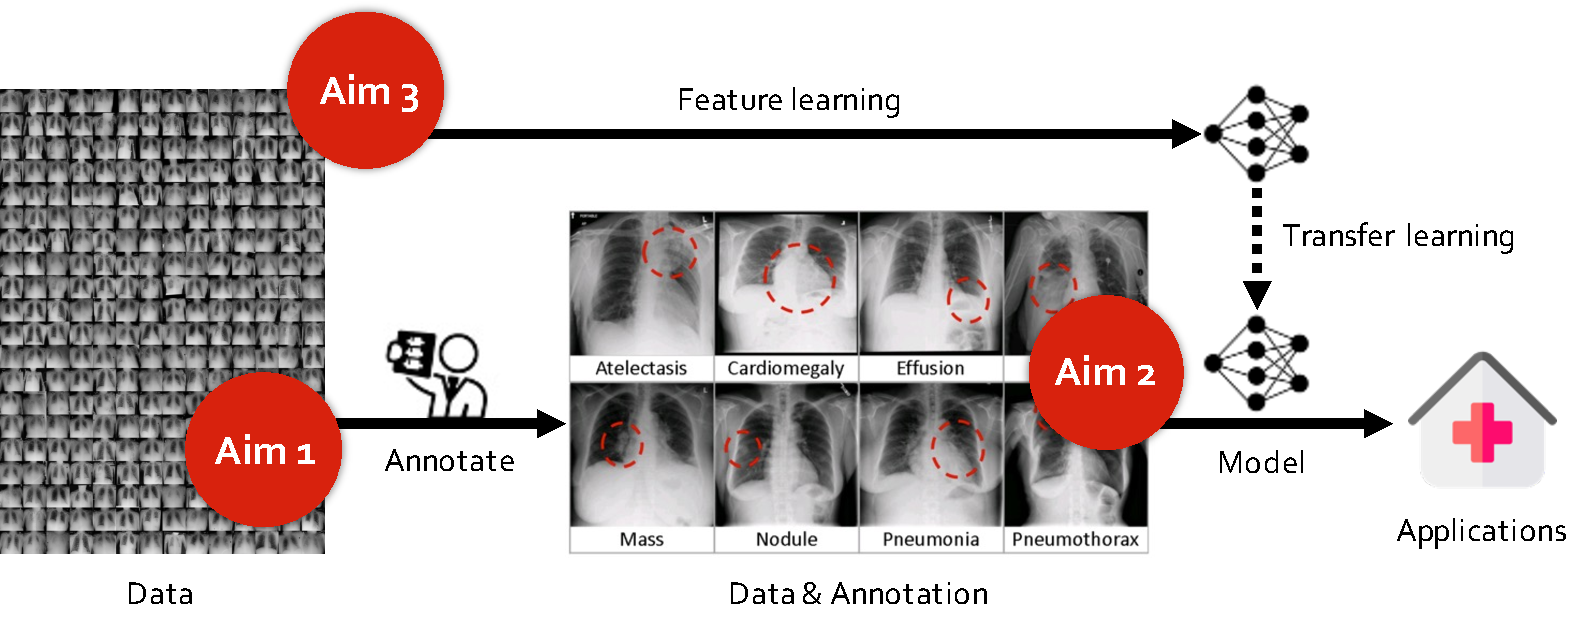
\includegraphics[width=1.0\linewidth]{Figures/CH1/fig_hypothesis.pdf}
\end{center}
\caption[Outline of the Dissertation]
{The overall pipeline of deep learning algorithms engaged in healthcare process: (1) obtaining annotation from human expert; (2) training and validating a deep model using these annotation; and (3) deploying the deep model in clinical practice. Our objective is to minimize manual annotation efforts for rapid, precise computer-aided diagnosis systems. In doing so, we have outlined three specific aims: (1) acquiring necessary annotation efficiently from human experts; (2) utilizing existing annotation effectively from advanced architecture; and (3) extracting generic knowledge directly from unannotated images. As a result, given the same amount of annotation, our deep learning models can yield higher performance; maintaining the similar performance, we ask for less annotation.}
\label{ch1:fig:hypothesis}
\end{figure}
%%%%%%%%%%%%%%%%%%%%%%%%%%%%%%%%%%%%%%%%%%%%


Annotating medical images is not only tedious and time consuming, but it also requires costly, specialty-oriented knowledge and skills, which are not easily accessible. To overcome this barrier, our objective is to develop innovative, annotation-efficient methodologies by exploiting the intrinsic characteristics of medical images. In this dissertation, we seek to address the critical problem: \textit{How to develop efficient and effective deep learning methods for medical applications where large annotated datasets are unavailable}.
The dream of ``big data'' induces the misconception that more data can promise higher performance, so we keep asking human experts to annotate as many data as possible. However, the performance of deep models is not linearly correlated to the number of annotated data; instead, there comes the plateau where even annotating more data cannot further improve the accuracy. This is due to the inevitable human error in annotation. Every task and model will encounter this bottleneck plateau. In essence, the amount of annotated data that can lead to the performance plateau is dependent on the complexity of the task, but it is also exceedingly influenced by the efficacy of the learning strategy and the capacity of the model architecture. This dissertation mainly focuses on optimizing the learning strategy and maximizing the model capacity, leading to our hypothesis that:

\bigskip\bigskip
\begin{tcolorbox}
With a small part of the dataset annotated, we can deliver deep models that match, or even outperform those that require annotating the entire dataset.
\end{tcolorbox}


We base this hypothesis on three pillars as outlined in~\figurename~\ref{ch1:fig:hypothesis}. First, wisely selecting important samples can reduce the annotation cost in comparison with random selection. A common procedure of determining which sample needs to be annotated first by human experts is called ``human-in-the-loop'' active learning. Second, multi-scale feature aggregation in deep models can address tasks with higher complexity. Image segmentation, as an example, is one of the most complicated tasks in medical image analysis, demanding rich image features that span levels from low to high, and scales from small to large. Finally, deep models with general-purpose image representation can be built upon the consistent, recurrent anatomical structure embedded in medical images. We envision that these generic models can serve as a primary source of transfer learning for many medical imaging tasks, even with limited annotated data. 


%%%%%%%%%%%%%%%%%%%%%%%%%%%%%%%%%%%%%%%%%%%%
\begin{figure}[t]
%\footnotesize
\begin{center}
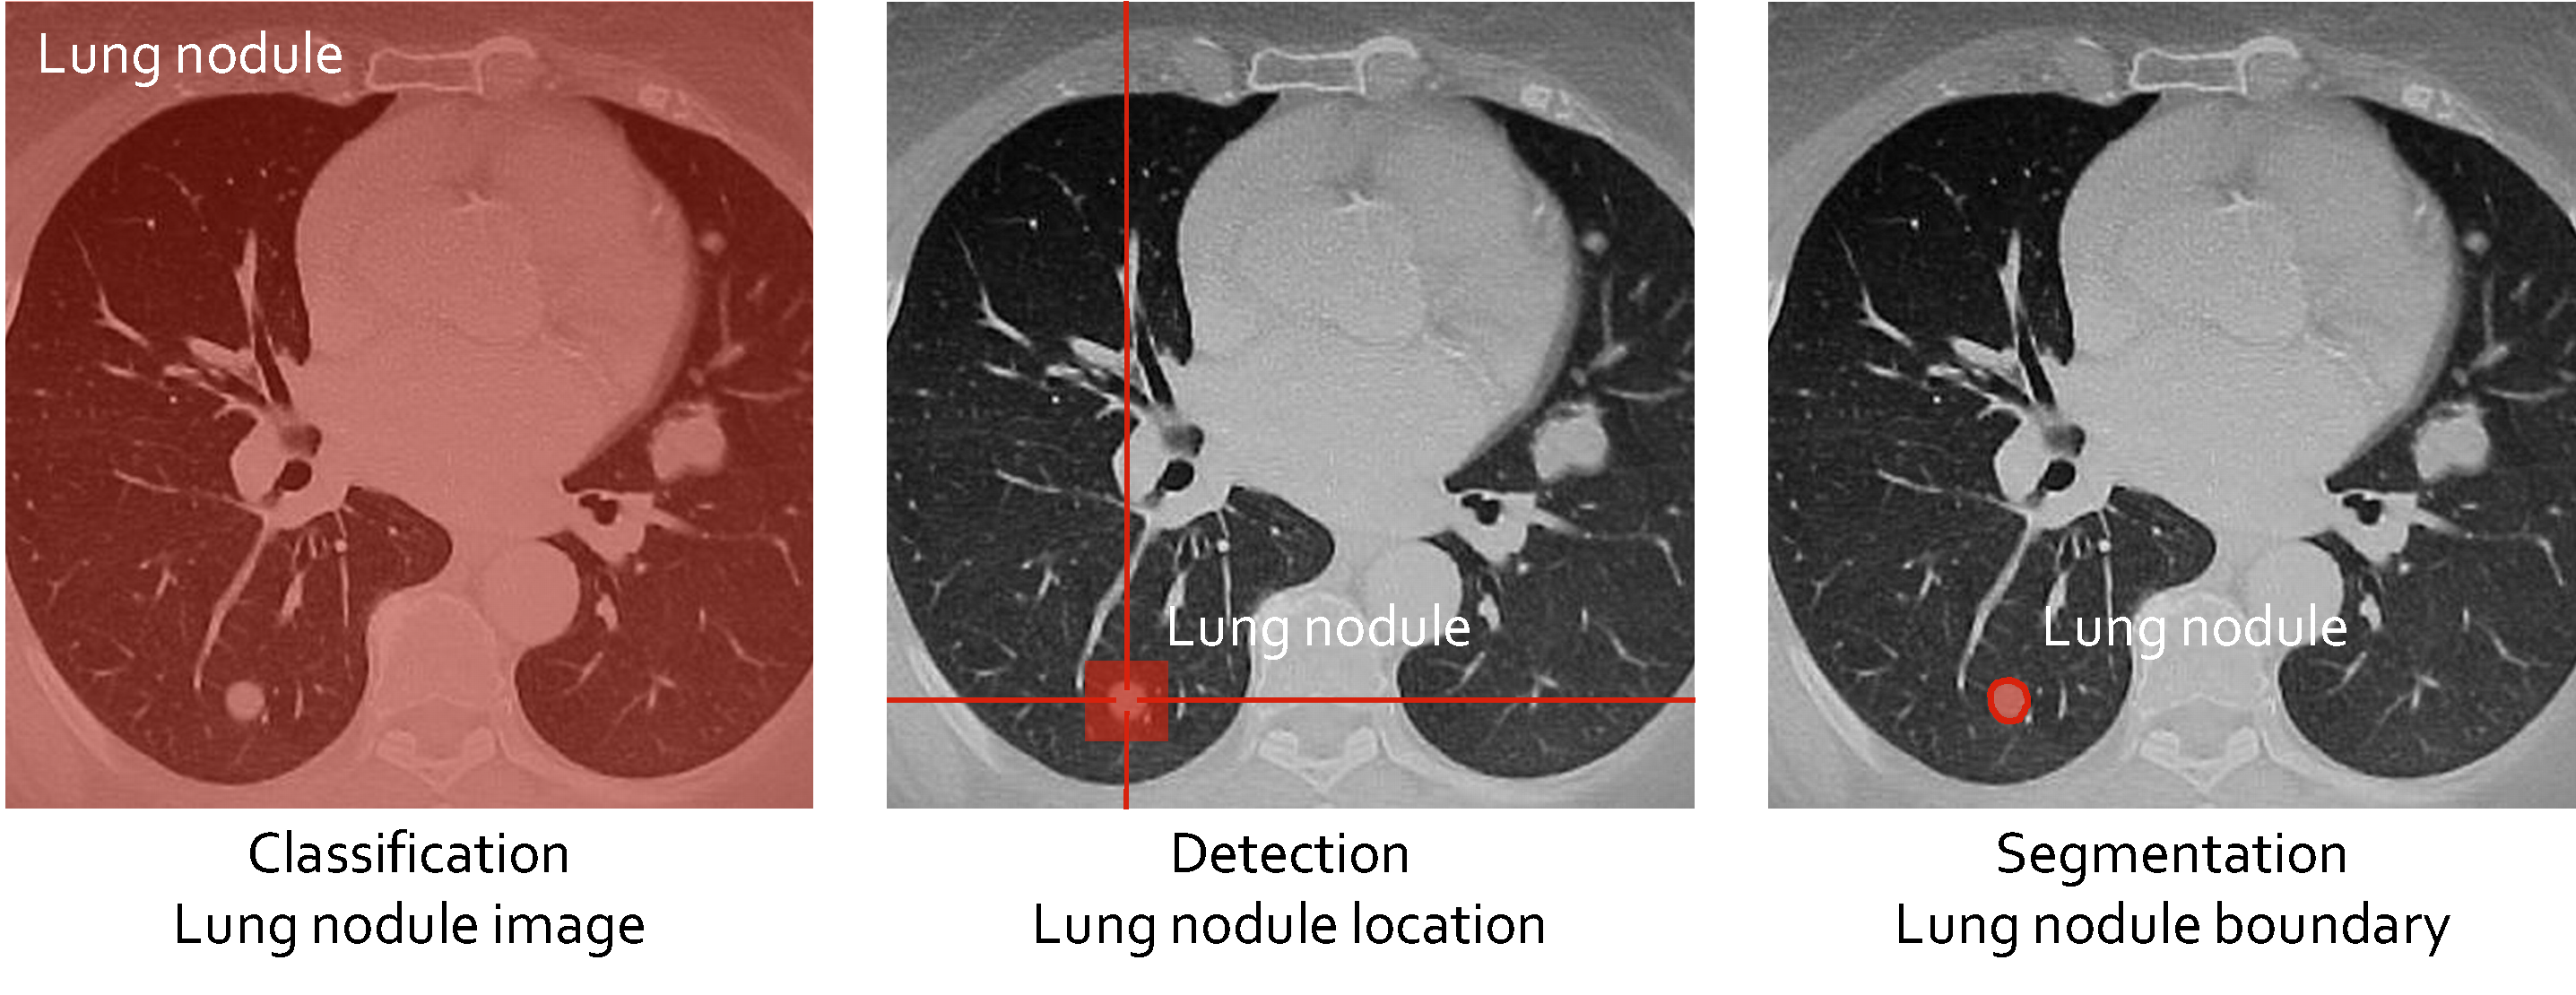
\includegraphics[width=1.0\linewidth]{Figures/CH1/fig_annotation_types.pdf}
\end{center}
\caption[What Is Annotation?]{
When harnessing large-scaled annotated datasets to advance medical imaging, the key question is \textit{what annotation should be collected}. There are several types of annotation as per the task requirements in clinical practice. Different types of annotation come with different associated costs. 
For example, to annotate lung nodules for the tasks of classification, detection, and segmentation, human experts must consider different types of annotation---labeling the existence of the nodule, indicating its location, and drawing a contour of its boundary, respectively. 
These three types of annotation are anticipated to span manual annotation efforts from easy to hard, annotation qualities from coarse to fine, and annotation time from short to long.}
\label{ch1:fig:annotation_types}
\end{figure}
%%%%%%%%%%%%%%%%%%%%%%%%%%%%%%%%%%%%%%%%%%%%


\section{What is Annotation?}
\label{ch1:challenge_opportunity:annotation}


Annotation is the process of assigning labels to raw data in preparation for training the computer on the pairs of data and labels; then, the computer can predict labels for many new data. For the development of deep learning methods, supervised learning is the most prominent learning paradigm, in which the annotation is used to guide model learning and error propagating. Therefore, annotating datasets is an indispensable stage of data processing in the AI era. For natural imaging, data is collected from numerous photos from social media and annotation is often given by non-experts through crowdsourcing~\citep{kovashka2016crowdsourcing}. Annotating medical images, however, demands costly, specialty-oriented knowledge and skills, which are not easily accessible. Thereby, medical image annotation is done mainly by human experts, who manually and precisely annotate the existence, appearance, and severity of diseases in each medical image with the help of appropriate software tools, such as Lionbridge AI, ITK-SNAP, Cogito, Labelbox, 3D Slicer, etc. For some abnormalities that experts cannot immediately recognize from images, biopsy outcomes can also be used as annotation. \figurename~\ref{ch1:fig:annotation_types} illustrates different types of annotation in medical imaging. This dissertation utilizes the annotation tagged with existing benchmark datasets as the gold standard to train and validate deep learning methods.



\section{The Barrier: Not Enough Annotation}
\label{ch1:challenge_opportunity:barrier}

Deep learning methods are data hungry by nature, requiring sufficiently large-scale, high-quality, well-integrated annotated datasets---more so than other algorithms. Recent studies suggest that, to match human diagnostic precision, deep learning methods require 42,290 radiologist-annotated CT images for lung cancer diagnosis~\citep{ardila2019end}, 137,291 radiologist-annotated mammograms images for breast cancer identification~\citep{mckinney2020international}, 129,450 dermatologist-annotated images for skin cancer classification~\citep{esteva2017dermatologist}, and 128,175 ophthalmologist-annotated retinal images for diabetic retinopathy detection~\citep{gulshan2016development}. Without such large annotated datasets, deep learning often results in algorithms that perform poorly and lack generalizability on new data. Nonetheless, rarely do we have a perfectly-sized and carefully-annotated dataset to train, validate, and test a deep learning model, particularly for applications in medical imaging, where both data and annotation are expensive to acquire. This requirement becomes more challenging in situations when quickly responding to global pandemics or when scaling up to several rare diseases where it is impractical to collect large quantities of annotated data. Manual annotation of medical images is still the key bottleneck in translating deep learning advancements into clinically useful computer-aided diagnosis (CAD) systems. Consequently, there is a pressing need for innovative methodologies that enable annotation-efficient deep learning for medical image analysis.






%In the following section, we extensively review the frontiers in technology that tackle the significant barrier of annotation acquisition by harnessing the three unique advantages, while demonstrating the novelty of the methodologies that we have developed.


\section{Overview of Contributions}
\label{ch1:thesis_outline}

This dissertation starts with a brief introduction of the concept of ``annotation'', followed by the motivation of developing annotation-efficient deep learning for computer-aided diagnosis. Specifically, we describe some of the greatest achievements of deep learning in medical imaging, associated with the number of annotation efforts behind these successes, underlining the desire to improve the efficiency of their development procedure. 


Chapter~\ref{ch2} compiles the role of annotation in developing computer vision algorithms from a historical perspective, shedding light on a discussion of current limitations and future premises. We then outline three unique advantages that have been stimulating the development of annotation-efficient deep learning for computer-aided diagnosis, including continual learning capabilities, representation learning capabilities, and recurrent anatomical structures. This chapter closes with an extensive review of how technical advancements address the barrier of annotation sparsity by harnessing the three unique advantages. Along the way, we highlight the novelty of the methodologies that we have developed by contrasting them with existing approaches. 


    
Chapter~\ref{ch3} discusses how to actively select patients/samples for annotation. We have devised a novel annotation query procedure to naturally integrate active learning and transfer learning into a single framework, reducing the manual annotation cost by at least half. Specifically, we combine newly annotated data with misclassified data by the current model, supplemented with continuous fine-tuning to accelerate model training, thereby encouraging the reuse of data. This procedure begins with a completely empty annotated dataset, improving the deep model's performance by actively selecting the most informative and representative samples. Studying different active learning strategies is important because an efficient ``human-in-the-loop'' procedure encourages label and model reuse, while additionally assisting radiologists in quickly dismissing patients with negative results. This work was one of only five papers in biomedical imaging accepted by CVPR-2017~\citep{zhou2017fine}. Consequently, this technique has been presented in several journal publications~\citep{zhou2019integrating,zhou2021active} and filed as a US patent application.
    
Chapter~\ref{ch4} discusses how to design advanced architectures that achieve annotation efficiency. We have designed an advanced neural architecture, named UNet++, for disease and organ segmentation, leveraging the power of existing annotation for improved performance. In doing so, we employed an efficient ensemble of U-Nets~\citep{falk2019u} of varying depths, which partially share an encoder and co-learn simultaneously using deep supervision, to alleviate the unknown network depth. 
We also redesigned skip connections to accommodate feature aggregation of varying semantic scales in decoder sub-networks. 
Finally, we devised a pruning scheme to accelerate model inference speed, allowing CAD systems to accomplish automatic disease detection using the ordinary desktop/laptop PCs commonly employed in clinical practice. This algorithmic innovation is significant because the learning capability of a deep model relies heavily on the use of multiple feature aggregation that can automatically learn representations from the data. UNet++ has been quickly adopted by the research community, listed among the most popular articles in IEEE TMI since published~\citep{zhou2018unet++,zhou2019unet++}; more recently, UNet++ has been widely applied to segment lung infections caused by COVID-19~\citep{dong2020role,shi2020review}. 
    
Chapter~\ref{ch5} discusses how to learn generic knowledge from unannotated data. We have developed a framework that trains generic source models for medical imaging, enabling rapid progress and improved performance for various medical applications across numerous diseases, datasets, organs, and modalities. This framework exploits an advantage stemming from the consistent and recurrent anatomy intrinsic to medical images that has the unique potential to act as strong, yet free, supervision signals for deep models to learn robust image representation. The self-supervised representation learning is beneficial to the research community because generic pre-trained models can serve as a primary source of transfer learning for numerous medical imaging applications, leading to accelerated training and improved performance. This work received the MICCAI Young Scientist Award\footnote{\href{http://www.miccai.org/about-miccai/awards/young-scientist-award/}{http://www.miccai.org/about-miccai/awards/young-scientist-award/}}~\citep{zhou2019models} and was chosen as one of the selected contributions, receiving the MedIA Best Paper Award in Medical Image Analysis\footnote{\href{http://www.miccai.org/about-miccai/awards/medical-image-analysis-best-paper-award/}{http://www.miccai.org/about-miccai/awards/medical-image-analysis-best-paper-award/}}~\citep{zhou2021models}.

Chapter~\ref{ch6} discusses how our developed techniques impact the key facets of CAD systems. We first describe some of the most distinguished characteristics of medical images, which are the vital foundations and inspirations of the techniques presented in this dissertation. We then express the clinical needs and introduce imaging applications in healthcare. Moreover, we dive into the details of how our techniques improve performance and annotation efficiency in an exemplar CAD system for detecting pulmonary embolism from CTPA images. Our system achieves a sensitivity of 46\% at 2 false positives per scan, ranked third among the participating teams in the CAD-PE competition.
    
Chapter~\ref{ch7} concludes the dissertation with a discussion of the overall impact. 
% {\jlred Not only for medical applications, but also other visual applications, such as.}


Many people criticize that deep learning requires too much annotated data, while humans can learn from one or a few examples---this argument is biased. It is true that training computers to detect lung nodules, for example, from CTs requires tens of thousands of annotated images~\citep{ardila2019end}, while a college student can accomplish the same task after being exposed to a few examples from textbooks. Nevertheless, we would not expect an infant to detect lung nodules by only seeing this small number of examples. The capability of annotation-efficient human vision (the holy grail for the next generation of deep learning) is based on numerous everyday learning activities. It takes a village to develop such annotation-efficient deep learning, and the resulting algorithm may not be prepared for any of the specific visual tasks. Once done, however, the algorithm can be quickly adapted to numerous tasks by only asking for a small amount of annotation, like human vision. As the popular Chinese saying goes, \textit{sharpening the axe will not slow down the work of cutting wood}. Progress in this line of research can leverage the power of small annotated data to establish more effective deep learning methods, therefore, alleviating the time and cost for manually annotating a large amount of data and exerting computer-aided diagnosis for a wider range of disorders.

% Annotation-efficient deep learning is the dream of computer vision and medical imaging, as it can significantly reduce the overall human annotation efforts, promoting computer-aided diagnosis for a wider range of disorders.

% Progress in this line of research can establish effective deep learning methods by leveraging small annotated data, therefore, dramatically reducing manual annotation efforts and exerting computer-aided diagnosis for a greater range of disorders.
\chapter{A Historical Review}
\label{ch2}

\section{The Role of Annotation}


As one of the most important subjects in artificial intelligence, computer vision enables computers to identify, perceive, and recognize people, places, and things, and ultimately imitate natural vision. The current state of computer vision is vulnerable to attack, unadaptable to new surroundings, and incapable of life-long learning. To match natural vision, our journey's just begun. 

\textit{Do we need annotation to develop human-like computer vision?} The necessity, formation, and quantity of annotation is fundamentally dependent on the learning objective---what do we wish the computer to learn?  An established learning objective can determine whether we should collect manual annotation and, if yes, what the type of the annotation is. For example, the learning objective of classifying 14 diseases requires the annotator to identify the types of diseases in the image; the learning objective of segmenting lung nodule requires the annotator to outline the boundary of each nodule. Defining the learning objective for specific imaging tasks is straightforward, but the learning objective for the task of matching natural vision is still inconclusive. This has led to spiraling debates on the necessity of acquiring manual annotation for developing human-like computer vision. In essence, the debates are about the learning objective of computer vision.

\subsection{Attribute Learning}

The earliest attempts to develop computer vision involved the idea that a visual concept (\eg cat) can be described and predicted by several attributes (\eg round face, chubby body, two pointy ears, and a long tail). If any object carries these preset attributes, the computer can identify cats from many images. While more advanced and sophisticated attributes arise, the underlying learning objective behind these approaches remains similar---identifying these descriptive attributes from the image. However, using these approaches, computers can make many simple mistakes, such as when (1) the objects are overlapping, (2) the object's position and shape are distorted, or (3) the object is conceptually difficult to define. The attribute-based approaches lack reliability, as countless concepts demand too much manual intervention for their definition and numerous variations that can eliminate the rule of conceptual modeling. To move away from extensive attribute engineering, researchers sought to automate feature learning for object recognition. 

\subsection{Categorical Learning}

Inspired by cognitive science and neuroscience, Drs.~Geoffrey~Hinton, Yann~LeCun, and Yoshua~Bengio developed an algorithm called deep neural networks~\citep{lecun1989backpropagation,bengio2009learning} that makes automated feature learning possible, but its strengths were not appreciated until the availability of big image datasets. At the beginning of 2007, Dr.~Fei-Fei~Li started creating a large-scale image dataset~\citep{deng2009imagenet}. She held the belief that developing reliable computer vision systems requires a lot of human annotated examples. Imagine a child's eyes as a pair of biological cameras, and they take one image about every 200 milliseconds. By age three, the child would have seen a tremendous number of real-world images. This observation promoted multiple large-scale, systematic-labeled datasets in the last few years. Deep neural networks trained on these datasets have enabled enormous advances in computer vision, leading to amazing results on some real-world tasks, such as object recognition, detection, segmentation, and image captioning. Additionally, in academic settings, deep neural networks almost always outperform alternative attribute-based approaches on benchmark tasks.

Combining large datasets, deep neural networks, and powerful computers, categorical supervised learning emerged as a new learning paradigm, where the learning objective for computers is to minimize the error between computer predictions and human labels. Here, humans play an essential role in training computers in this learning paradigm because humans must provide all categorical labels for the dataset. Although training deep neural networks using categorical supervised learning is quite effective, there are three inherent restrictions: (1) computers can only differentiate the specific categories given by humans, but not beyond; (2) computers can perform poorly on real-world images outside the dataset; and, most importantly, (3) the resulting computer vision is much less general, flexible, and adaptive than natural vision. Categories and concepts in the real world can be far more comprehensive than those given in the benchmark datasets. It is because the categories in the real world are non-orthogonal (cat and tiger vs. cat and plane), imbalanced (long-tail distribution for most classes), and exponential (classes with hierarchical sub-classes). Since a computer is unable to learn categories beyond what has been given, the annotating work can keep going on indefinitely, and the resultant computer vision would always be tied with specific categories. The categorical supervised learning paradigm is essentially the same as attribute-based learning, where categories serve as attributes to help computers understand the world. 


The major concern is not the challenge to annotate an adequate number of images but rather the fact that learning paradigms are fundamentally asymmetrical between computer vision and natural vision, in which the former is currently built upon categorical labels while the latter is developed from images without any label. Human babies and animals establish vision naturally without direct supervision---in nature, there is no dictionary of concepts available---they learn these through real-world experiences and interactions. Although the top-down categorization, based on a linguistic definition, can help develop task-specific computer vision systems, it might be unnecessary for a general-purpose visual system. To deal with the enormous complexity of natural images and obtain the rich understanding of visual scenes that the human achieves, today, we still yearn to know the underlying objective of natural vision~\citep{yuille2021deep}. 

\subsection{Representation Learning}

The dissimilarity between natural vision and current computer vision suggests alternative learning paradigms. Self-supervised learning is an interesting reflection on the general thought on learning representation in a way similar to natural vision. This learning paradigm has existed for some time, but its power historically has lagged behind the state-of-the-art categorical supervised learning. However, the recent pace of progress in self-supervised learning has increased dramatically and led to visual representation that approaches and even surpasses the representation learned from supervised categorization. It has raised hopes that self-supervised learning could indeed replace the ubiquitous categorical supervised learning in advanced computer vision going forward. Unlike categorical supervised learning, a computer does not have to learn orthogonal, balanced, and finite categories from human annotation; instead, it learns by studying the properties of real-world images. Self-supervision promises to get away from top-down categorization and enable continuous life-long learning. As highly advocated by Drs. Yann LeCun and Yoshua Bengio, ``self-supervised learning is the key to human-level intelligence.''~\citep{wiggers2020yann}

The line of research on self-supervision is more closely investigating the objective of natural vision development. As a learner interacts with the environment, one of the most common objectives is to survive---to avoid either being attacked or starving---which has led to two major research avenues in self-supervision: (1) learning a predictive model to fill in the blank and (2) learning a contrastive model to distinguish multiple views. First, to prevent being attacked or killed, a learner should develop meaningful expectations about the world, coming up with a hypothesis of the world and then verifying it. As a result, the predictive model predicts some hidden information (\eg color, future events, or contexts of an image) to perceive prior knowledge and physical properties in nature, such as the sky being blue or a running beast approaching you. Second, to ensure survival, a learner is expected to distinguish objects (\eg determining food edibility based on color, shape, texture, etc.). It should be noted that distinguishing is different from categorizing because the distinction can separate things even if they belong to the same category. Consequently, instead of categorization, the contrastive model compares images that have undergone strong data augmentation to learn image representation, which is resilient to various view changes.

\subsection{Current Limitations and Future Considerations}

In the discussion above, we have been following a similar principle to develop general-purpose computer vision: \textit{do not define anything}. While learning algorithms are continually changing as better methods are developed, one trend that is not going away is the move towards increased levels of automation. We seek for a way to let computers autonomously interact with images and capture visual representation, keeping away from manually defining attributes, categories, etc. Automated feature learning will save time, build generic models, create meaningful features, and encourage learning from diverse data sources. As of now, compared with natural vision, the current state of self-supervision is incomplete in at least three ways.

\begin{itemize}
    \item \textit{First, the choice of augmented views is supervised by humans.} Data augmentation is widely used for training both predictive and contrastive models due to its simplicity and efficiency. A predictive model restores the original images from the transformed ones through data augmentation; a contrastive model distinguishes the same image from different views generated from data augmentation. However, humans must pre-define a set of data augmentations specific to each task because some augmentations can make a task ambiguous, unsolvable, or trivial, leading to degenerate learning. Here comes several examples: cropping patches from images can occlude the target object; permutating color is mostly not applicable to grayscale images; predicting rotation angles in medical images can be trivial due to the consistent anatomical structure. Many recent works appear to automate data augmentation in self-supervised learning, one of which is to use videos rather than images. Humans learn from a sequence of meaningful images instead of a large number of non-related still images because videos naturally associate with different continuous views. Another way is to use generated images so that bottleneck features can manipulate the image context to ensure target objects' existence.
    
    \item \textit{Second, the choice of model architectures is supervised by humans.} In the existing literature, methods are generally developed to learn the weights (parameters) of a fixed architecture without using labels, and these weights are evaluated by transferring to a target supervised task. In a recent study, \citet{liu2020labels} explored the possibility of using such methods to learn architecture without using labels. The neural architecture search seems to relax the manual design, but the search space heavily relies on humans. There are three challenges associated with the existing approaches. (1) The neural connection can never be found if it is not included in the original search space—the search space limits what neural architecture can be discovered. (2) The searching will terminate into a fixed architecture if it meets a local minimum. In contrast, the neural connection in human brains is dynamically evolving throughout the lifespan. (3) Vast computational resources are required for the neural architecture search, while the resultant architecture cannot guarantee superior outcomes to human-engineered architectures~\citep{isensee2021nnu}. In addition, although convolutional neural networks are currently dominant in most imaging tasks, another architecture called transformer was proven more powerful to encode long-term dependencies among data~\citep{vaswani2017attention,dosovitskiy2020image}, therefore exceeding in analyzing sequences of data such as language and video.
    
    \item \textit{Third, the choice of pretext tasks is supervised by humans.} That being said, a wide range of learning schemes with varying learning objectives are currently designed by humans, such as predicting rotation, augmentation, color, etc~\citep{jing2020self}. But the fact is, we are unsure how exactly natural vision is developed, as we are the users, not the designers. It is possible that pre-defined learning schemes, either filling in blanks or contrasting views, could dilute the true power of self-supervised learning. Given an image, human vision is developed by multi-tasking, such as depth estimation, motion prediction, orientation perception, object detection, etc. The types of these tasks are not pre-defined but driven by an underlying objective. We have given special prominence to the objective that drives a learner to develop vision because it is the learning objective that mostly makes such diverse types of tasks for us to learn, even though sometimes our supervisors (parents, teachers, primers) suggest some specific tasks for us. Instead of devising many pretext tasks, the real mission is to figure out the true objective beyond vision, which comes up with a research field called learning to learn or meta learning~\citep{lake2015human}. According to the concept of meta learning, a learner itself must be exposed to a large number of tasks and tested on their ability to learn new tasks. Thus, humans do not have to design which tasks to solve, and instead, computers make up their own games to develop computer vision.
\end{itemize}


As revealed in a historical review, it remains an open problem to construct a complete, unified learning objective of computer vision using one concise equation. In the past decades, we have made exciting progress by discovering partial learning objectives that make computers accomplish specific tasks and developing critical components that collectively simulate natural vision. We are heading towards the direction where the advancements in computer vision rely less and less on manual annotation to secure comprehensive visual knowledge from images. 
% Finally, we have outlined three future premises for promoting annotation-efficient deep learning, which places a great ending point of my incredible Ph.D. journey and opens a new chapter for future exploration.


\section{The Opportunity: Annotation-Efficient Deep Learning}
\label{ch2:challenge_opportunity:opportunity}

% {\jlred Why annotation-efficient deep learning is an opportunity?}
This section overviews three advantages that have stimulated annotation-efficient deep learning and resulted in numerous emerging subjects, including our contributions in this dissertation. 

\begin{enumerate}
    \item \textit{The continual learning capabilities of deep learning incrementally improve the algorithm through fine-tuning.} Millions of new medical images are generated in hospitals every day. With such a colossal stream of data, it is impracticable to store the data in memory and repeatedly train computers from scratch once new data becomes available. We hope computers to leverage the prior knowledge obtained from old data over time and continuously accommodate new data, like human beings. Continual learning is built on the idea that learners adaptively use new data so their knowledge sets can develop autonomously and incrementally. The continual learning ability is one of the critical benefits that deep learning could offer. Unlike conventional machine learning methods, deep learning models can be fine-tuned on top of previously learned weights that often store the memories and knowledge of old data. Specifically, we can take a set of trained weights and use it as model initialization for new data. The ability of continual learning would be much more appreciated in the scenario of the ``human-in-the-loop'' procedure, wherein human experts interact with computers to promote the development of algorithms using a continuous stream of data. An efficient ``human-in-the-loop'' procedure helps human experts quickly dismiss patients with negative results, therefore, dramatically reducing the burden of annotation. Moreover, an instant online feedback process encourages data, annotation, and model reuse, making it possible for CAD systems to self-improve via continual fine-tuning.
    
    \item \textit{The representation learning capabilities of deep learning alleviate exhaustive feature engineering for specific medical conditions.} Feature engineering manually designs features based on the texture and shape present in images, which are easier to describe and troubleshoot so humans can manipulate features on their own. However, crafting such features demands a great deal of patience, diligence, and expertise. Most hand-crafted features focus on specific medical conditions, hence greatly limiting the expressive powers and depreciating the generalization capacity. For instance, radiomics features can be beneficial in radiological imaging, but they are not adaptable to other imaging modalities, such as dermatology, histopathology, and ophthalmology. Recent deep learning methods swept away previous hand-crafted features, showing that neural networks can solve diverse tasks by automatically learning hierarchical features at multiple levels of abstraction. In networks, each layer projects the image into a particular feature space---the deeper layer generates a higher level of abstraction by extracting more complex features built on top of simpler ones. The merit of deep learning is that the varying levels of features are not manually designed by humans. For this, we call it ``representation learning'', a procedure that automatically learns visual features to represent an image. Representation learning is more efficient and repeatable than exhaustive feature engineering, saving tremendous amounts of manual work. Compared with hand-crafted features, deep features offer four advantages: (1) deep features can be dynamically computed by models during training and test stages; (2) deep features present a semantic hierarchy, varying from layer to layer; (3) deep features can be used for not only classification but also registration, localization, and segmentation; (4) deep features can be fine-tuned and adapted to different tasks and domains. Many studies have reaffirmed that automated feature learning can produce more generalizable image representation than hand-crafted features.
    
    \item \textit{The consistent and recurrent anatomy embedded in medical images empowers deep learning with a generic visual representation.} Human anatomies are intrinsically structured, exhibiting consistency in appearance, position, and layout. Medical imaging protocols focus on particular parts of the body, often generating images of great similarity and yielding an abundance of sophisticated anatomical patterns across patients. These patterns are naturally associated with comprehensive knowledge about human anatomy. Therefore, consistent and recurrent anatomy can ease the analysis of numerous critical problems and should be considered a significant advantage of medical imaging. Due to the recurring anatomy, the same body parts in different images express similar visual patterns and, therefore, can be retrieved by what is known as ``nearest neighbor search''. As a result, given a single annotated medical image, similar anatomical patterns can be found in many other images so that radiologists can track disease progress with landmark detection and lesion matching. In addition to correspondence matching, the recurrent anatomical structures in medical images are associated with rich knowledge about the human body and intrinsic structural coherence, offering great benefit and potential to foster image representation and produce more powerful source models. Consequently, one-shot or few-shot learning in various medical applications would be eventually actualized. 
\end{enumerate}


\section{Related Work \& Our Innovations}
\label{ch1:related_work}


We extensively review the related work that tackles the significant barrier of annotation sparsity by harnessing the three unique advantages, while underlining the novelty of the methodologies that we have developed.

\subsection{Acquiring Necessary Annotation}
\label{ch1:related_work:acquiring_necessary_annotations}

\subsubsection{One-time learning and continual learning}
\label{ch1:related_work:acquiring_necessary_annotation:transfer_learning_medical_imaging}

Pre-training a model on large-scale image datasets and then fine-tuning it on various target tasks has become a \textit{de facto} paradigm across many medical specialties. As summarized by~\citet{irvin2019chexpert}, to classify the common thoracic diseases on chest radiography, nearly all the leading approaches~\citep{guan2018multi,guendel2018learning,tang2018attention,ma2019multi} follow this paradigm by adopting different architectures along with their weights pre-trained from ImageNet. Other representative medical applications include identifying skin cancer from dermatologist level photographs~\citep{esteva2017dermatologist}, diagnosing Alzheimer's Disease~\citep{ding2018deep} from $^{18}$F-FDG PET of the brain, and performing effective detection of pulmonary embolism~\citep{tajbakhsh2019computer} from CTPA. 
Recent breakthrough in self-supervised pre-training~\citep{grill2020bootstrap,caron2020unsupervised,chen2020exploring}, on the other hand, has led to visual representation that approaches and possibly surpasses what was learned from ImageNet. Self-supervised pre-training has also been adopted for the medical domain, wherein \citet{zhou2019models,zhu2020rubik,feng2020parts2whole,haghighi2020learning,azizi2021big} develop generic CNNs that are directly pre-trained from medical images, mitigating the mandatory requirement of expert annotation and reducing the large domain gap between natural and medical images. Despite the immense popularity of transfer learning in medical imaging, these works exclusively employed {\em one-time fine-tuning}---simply fine-tuning a pre-trained CNN,  for only one time, with available training samples. In real-world applications, instead of training on a still dataset, experts record new samples constantly and expect the samples to be used upon their availability. Therefore, by empowering the CNN with the ability to deal with new data, continual learning is the bridge to active and open world learning~\citep{mundt2020wholistic}. Compared with the existing continual learning approaches~\citep{kading2016fine,zhou2017fine}, our newly devised learning strategy is more amenable to active fine-tuning because it focuses more on the newly annotated samples and also recognizes those misclassified ones, eliminating repeated training on easier samples in the annotated pool.


\subsubsection{Integrating active learning with deep learning}
\label{ch1:related_work:acquiring_necessary_annotation:integrating_active_learning_deep_learning}


The uncertainty and diversity are the most compelling active selection criteria, which appraise the worthiness of annotating a sample from two different aspects. Uncertainty-based criteria argue that the more uncertain a prediction is, the more value added when including the label of that sample into the training set. Sampling with least confidence~\citep{culotta2005reducing}, large entropy~\citep{dagan1995committee,mahapatra2018efficient,shao2018deep,kuo2018cost}, or margins~\citep{scheffer2001active,balcan2007margin} of the prediction has been successful in training models with fewer labels than random sampling. The limitation of uncertainty-based criteria is that some of the selected samples are prone to redundancy and outliers~\citep{sourati2019intelligent} and may not be representative enough for the data distribution as a whole. Alternatively, diversity-based criteria have the advantage of selecting a set of most representative samples, related to the annotated ones, from those in the rest of the unannotated set. The intuition is it is unnecessary to repeatedly annotate similar samples. Mutual information~\citep{li2013adaptive,gal2017deep}, Kullback-Leibler divergence~\citep{kulick2014active,mccallumzy1998employing}, Fisher information~\citep{sourati2018active,sourati2019intelligent}, K-centers and core sets~\citep{sener2017active}, calculated among either model predictions or image features, are often used to ensure the diversity. Although alleviating redundancy and outliers, a serious hurdle of diversity-based criteria is the computational complexity for a large pool of unannotated samples. We address this issue by measuring diversity over patches augmented from the same sample, making the calculation much more manageable. To exploit the benefits and potentials of the two selecting aspects, the studies of \citet{wang2018deep,ozdemir2018active,mahapatra2018efficient,shui2020deep} consider the mixture strategy of combing uncertainty and diversity explicitly. \citet{yang2017suggestive,beluch2018power,kuo2018cost} further compute the selection criteria from an ensemble of CNNs---these approaches are, however, very costly in computation, as they must train a set of models to compute their uncertainty measure based on models' disagreements. For additional active learning methods, we refer the reader to comprehensive literature reviews~\citep{tajbakhsh2020embracing,munjal2020towards,hino2020active,ren2020survey}; but these existing methods are fundamentally different from our active continual fine-tuning (ACFT) in that they all repeatedly re-trained CNNs from scratch at each step, whereas we continually fine-tune the (fine-tuned) CNN incrementally. As a result, our ACFT offers several advantages as listed in Sec.~\ref{ch3:approach_property:several_unique_properties}, and leads to dramatic annotation cost reduction and computation efficiency. Besides, we have found that there are only seven fundamental patterns in CNN predictions, as summarized in~\tablename~\ref{ch3:tab:predict_pattern}. Multiple methods may be developed to select a particular pattern: entropy, Gaussian distance, and standard deviation would seek Pattern A, while diversity, variance, and divergence look for Pattern C. We were among the first to analyze the prediction patterns in active learning and investigate the effectiveness of typical patterns rather than comparing the many methods. 


% \subsection{Medical image segmentation}
\subsection{Designing Advanced Architectures}
\label{ch1:related_work:designing_advanced_architectures}

% In the following, we review the works related to redesigned skip connections, feature aggregation, and deep supervision, which are the main components of our new architecture.

\subsubsection{Skip connections}
\label{ch1:related_work:designing_advanced_architectures:skip_connections}

Skip connections were first introduced in the seminal work of
\citet{long2015fully} where they proposed fully convolutional networks (FCN) for semantic segmentation. Shortly after, building on skip connections, \citet{ronneberger2015u} proposed U-Net architecture for semantic segmentation in medical images. The FCN and U-Net architectures, however, differ in how the decoder features are fused with the same-scale encoder features. While FCN~\citep{long2015fully} uses the summation operation for feature fusion,  U-Net~\citep{ronneberger2015u} concatenates the features followed by the application of convolutions and non-linearities. The skip connections have shown to help recover the full spatial resolution, making fully convolutional methods suitable for semantic segmentation~\citep{chaurasia2017linknet,lin2017refinenet,zhao2018icnet,tajbakhsh2020errornet}. 
Skip connections have further been used in modern neural architectures such as  residual networks~\citep{he2016deep,he2016identity} and dense networks~\citep{huang2017densely}, facilitating the gradient flow and improving the overall performance of classification networks.

\subsubsection{Aggregating multi-scale features}
\label{ch1:related_work:designing_advanced_architectures:feature_aggregation}
The exploration of aggregating hierarchical features continues to be a popular subject of research. \citet{fourure2017gridnet} propose GridNet, which is an encoder-decoder architecture wherein the feature maps are wired in a grid fashion, generalizing several classical segmentation architectures. Despite GridNet containing multiple streams with different resolutions, it lacks up-sampling layers between skip connections; and thus, it does not represent UNet++.
Full-resolution residual networks (FRRN)~\citep{pohlen2017full} employs a two-stream system, where full-resolution information is carried in one stream and context information in the other pooling stream. In~\citet{jiang2019multiple}, two improved versions of FRRN are proposed, \ie incremental MRRN with 28.6M parameters and dense MRRN with 25.5M parameters. 
These 2D architectures, however, have similar number of parameters to our 3D VNet++ and three times more parameters than 2D UNet++; and thus, simply extending these architectures to a 3D manner may not be amenable to the common 3D medical applications.
We would like to note that our redesigned dense skip connections are completely different from those used in MRRN, which consists of a common residual stream. Also, it is not flexible to apply the design of MRRN to other backbone encoders and meta framework such as Mask R-CNN~\citep{he2017mask}. Deep layer aggregation (DLA)~\citep{yu2018deep}, topologically equivalent to our intermediate architecture UNet+ (\figurename~\ref{ch4:fig:network_architecture}(f)), adjacently connects the same resolution features without U-Net's long skip connections. Our experimental results demonstrate that by densely connecting the layers, UNet++ achieves higher segmentation performance than UNet+/DLA (see \tableautorefname~\ref{ch4:tab:main_results}). 

\subsubsection{Introducing deep supervision}
\label{ch1:related_work:designing_advanced_architectures:deep_supervision}

He~\etal~\citep{he2016deep} suggested that the depth of network can act as a regularizer. Lee~\etal~\citep{lee2015deeply} demonstrated that deeply supervised layers can improve the learning ability of hidden layers, enforcing the intermediate layers to learn discriminative features, enabling  fast convergence and regularization of the network~\citep{dou20173d}. DenseNet~\citep{huang2017densely} performs a similar deep supervision in an implicit fashion. Deep supervision can also be used in U-Net like architectures.
\citet{dou20163d} introduce deep supervision by combining predictions from varying resolutions of feature maps, suggesting that it can combat potential optimization difficulties, and thus, reach a faster convergence rate and more powerful discrimination capability. \citet{zhu2017deeply} used eight additional deeply supervised layers in their proposed architecture. 
Our nested networks, however, are more amenable to training under deep supervision: 1) multiple decoders automatically generate full resolution segmentation maps; 2) the networks are embedded at various different depths of U-Net so that it grasps multi-resolution features; 3) densely connected feature maps help smooth the gradient flow and give a relatively consistent predicting mask; 4) the high dimension features have effects on all of the outputs through back-propagation, allowing us to prune the network in the inference phase.


% \subsection{Representation learning}
\subsection{Extracting Generic Image Features}
\label{ch1:related_work:extracting_generic_image_features}

With the splendid success of deep neural networks, transfer learning~\citep{pan2010survey,weiss2016survey,yosinski2014transferable} has become integral to many applications, especially medical imaging~\citep{greenspan2016guest,litjens2017survey,lu2017deep,shen2017deep,wang2017comparison,zhou2017fine,zhou2019models,zhou2021models}. This immense popularity of transfer learning is attributed to the learned image representation, which offers convergence speedups and performance gains for most target tasks, in particular, with limited annotated data. In the following sections, we review the works related to supervised and self-supervised representation learning.

\subsubsection{Supervised representation learning} 

%Annotating data at this scale required a significant research effort and budget, and was achieved using crowdsourcing platforms. It is not feasible to create annotated datasets of this size for every application.

ImageNet contains more than fourteen million annotated images that indicate which objects are present; and more than one million of the images have actually been annotated with the bounding boxes of the objects. Pre-training a model on ImageNet and then fine-tuning it on other imaging tasks has seen the most practical adoption in medical image analysis~\citep{bar2015chest,shin2016deep,tajbakhsh2016convolutional}. Despite its remarkable transferability, the 2D ImageNet model offers little benefit towards 3D medical imaging tasks in the most prominent medical modalities (\eg CT and MRI). To fit this paradigm, 3D imaging tasks have to be reformulated and solved in 2D~\citep{roth2015improving,roth2014new,tajbakhsh2015computer}, thus losing rich spatial information and inevitably compromising the performance. Annotating 3D medical images at a similar scale with ImageNet requires a significant research effort and budget. It is currently infeasible to create annotated datasets comparable to this size for every 3D medical application. 
Consequently, for lung cancer malignancy estimation, \citet{ardila2019end} resorted to incorporate spatial information by using Inflated 3D~\citep{carreira2017quo}, trained from the Kinetics dataset, as the feature extractor. Evidenced by \tablename~\ref{ch5:tab:top_existing_models}, it is a suboptimal choice due to the large domain gap between the temporal video and medical volume. This limitation has led to the development of the NiftyNet model zoo~\citep{gibson2018niftynet}. However, they were trained with small datasets for specific applications (\eg brain parcellation and organ segmentation), and were never intended as source models for transfer learning. Our experimental results, in \tablename~\ref{ch5:tab:top_existing_models}, indicate that NiftyNet models offer limited benefits to the five target medical applications via transfer learning. More recently, \citet{chen2019med3d} have pre-trained 3D residual networks by jointly segmenting the objects annotated in a collection of eight medical datasets, resulting in MedicalNet for 3D transfer learning. In \tablename~\ref{ch5:tab:top_existing_models}, we have examined the pre-trained MedicalNet on five target tasks in comparison with our Models Genesis. As reviewed, each and every aforementioned pre-trained model requires massive, high-quality annotated datasets. However, seldom do we have a perfectly-sized and systematically-annotated dataset to pre-train a deep model in medical imaging, where both data and annotation are expensive to acquire. We overcome the above limitation by using self-supervised learning, which allows models to learn image representation from abundant unannotated medical images with {\em zero} human annotation effort.

\subsubsection{Self-supervised representation learning}

Aiming at learning image representation from unannotated data, self-supervised learning research has recently experienced a surge in computer vision~\citep{caron2018deep,chen2019rotation,doersch2015unsupervised,goyal2019scaling,jing2020self,mahendran2018cross,mundhenk2018improvements,noroozi2018boosting,noroozi2016unsupervised,pathak2016context,sayed2018cross,zhang2016colorful,zhang2017split}, but it is a relatively new trend in modern medical imaging. The key challenge for self-supervised learning is identifying a suitable task that generates input and output instance pairs from the data. Two of the preliminary studies include (1) predicting the distance and 3D coordinates of two patches randomly sampled from the same brain~\citep{spitzer2018improving} and (2) identifying whether two scans belong to the same person and further predicting the level of vertebral bodies~\citep{jamaludin2017self}. Nevertheless, these two works are incapable of learning representation from ``self-supervision'' because they demand auxiliary information and specialized data collection such as paired and registered images. By utilizing only the original pixel/voxel information shipped with data, several self-supervised learning schemes have been developed for different medical applications: \citet{ross2018exploiting} adopted colorization as the proxy task, wherein color colonoscopy images are converted to gray-scale and then recovered using a conditional Generative Adversarial Network (GAN); \citet{alex2017semisupervised} pre-trained a stack of denoising auto-encoders, wherein the self-supervision was created by mapping the patches with the injected noise to the original patches; \citet{chen2019self} designed image restoration as the proxy task by first shuffling small regions of the image and then training the model to restore the original image; \citet{zhuang2019self} and \citet{zhu2020rubik} introduced a 3D representation learning proxy task by recovering the rearranged and rotated Rubik's cube; and finally \citet{tajbakhsh2019surrogate} individualized self-supervised schemes for a set of target tasks. As seen, the previously discussed self-supervised learning schemes, both in computer vision and medical imaging, are developed individually for specific target tasks; therefore, the generalizability and robustness of the learned image representation have yet to be examined across multiple target tasks. To our knowledge, we are the first to investigate cross-domain self-supervised learning in medical imaging. 
\chapter{Acquiring Annotation from Human Experts}
\label{ch3}

This chapter is based on the following publications:
\begin{itemize}
    \item Zhou, Z., Shin, J., Zhang, L., Gurudu, S., Gotway, M., \& Liang, J. (2017). Fine-tuning convolutional neural networks for biomedical image analysis: actively and incrementally. In \textit{Proceedings of the IEEE conference on computer vision and pattern recognition} (pp. 7340-7351).
    \item Zhou, Z., Shin, J., Feng, R., Hurst, R. T., Kendall, C. B., \& Liang, J. (2019). Integrating active learning and transfer learning for carotid intima-media thickness video interpretation. \textit{Journal of digital imaging}, 32(2), 290-299.
    \item Zhou, Z., Shin, J. Y., Gurudu, S. R., Gotway, M. B., \& Liang, J. (2021). Active, Continual Fine Tuning of Convolutional Neural Networks for Reducing Annotation Efforts. \textit{Medical Image Analysis}, 101997.
\end{itemize}

% \section*{CRediT authorship contribution statement}

% I would like to thank all of the authors for their contributions and hard works. Jae Y. Shin: software, investigation, visualization. Suryakanth R. Gurudu: resources, data curation. Michael B. Gotway: resources, data curation, funding acquisition. Jianming Liang: conceptualization, methodology, formal analysis, investigation, resources, writing, supervision, project administration, funding acquisition. 

\newpage


\section{Background \& Motivation}
\label{ch3:backgroun_motivation}

Convolutional neural networks (CNNs)~\citep{lecun2015deep} have ushered in a revolution in computer vision owing to the use of large annotated datasets, such as \textsc{ImageNet}~\citep{deng2009imagenet} and \textsc{Places}~\citep{zhou2017places}. As evidenced by two recent books~\citep{shen2019medical,zhou2019handbook} and numerous compelling techniques for different imaging tasks~\citep{moen2019deep,yamamoto2019automated,ravizza2019predicting,esteva2019guide,huang2020penet,isensee2021nnu}, there is widespread and intense interest in applying CNNs to medical image analysis, but the adoption of CNNs in medical imaging is hampered by the lack of such large annotated datasets. Annotating medical images is not only tedious and time consuming, but it also requires costly, specialty-oriented knowledge and skills, which are not readily accessible. Therefore, we seek to answer this critical question: {\em How to dramatically reduce the cost of annotation when applying CNNs to medical imaging}?
In doing so, we have developed a novel method called ACFT (active, continual fine-tuning) to naturally integrate active learning and transfer learning into a single framework. Our ACFT method starts directly with a pre-trained CNN to seek ``salient'' samples from the unannotated pool for annotation, and the (fine-tuned) CNN is continually fine-tuned using newly annotated samples combined with all misclassified samples. We have evaluated our method in three different applications, including colonoscopy frame classification, polyp detection, and pulmonary embolism (PE) detection, demonstrating that the cost of annotation can be reduced by at least half.

This performance is attributable to a simple yet powerful observation: to boost the performance of CNNs in medical imaging, multiple patches are usually generated automatically for each sample through data augmentation; these patches generated from the same sample share the same label, and are naturally expected to have similar predictions by the current CNN before they are expanded into the training dataset. As a result, their {\em entropy}~\citep{shannon1948mathematical} and {\em diversity}~\citep{kukar2003transductive} provide a useful indicator of the ``power'' of a sample for elevating the performance of the current CNN. However, automatic data augmentation inevitably generates ``hard'' samples, injecting noisy labels. Therefore, to significantly enhance the robustness of active selection, we compute entropy and diversity from only a portion of the patches according to the majority predictions detailed in Sec.~\ref{ch3:approach_property:handling_noisy_labels_majority_selection}) by the current CNN. 
Furthermore, to strike a balance between exploration and exploitation, we incorporate randomness in our active selection as detailed in Sec.~\ref{ch3:approach_property:injecting_randomization_active_selection}; and to prevent catastrophic forgetting, we combine newly selected samples with misclassified samples as described in Sec.~\ref{ch3:experiment_result:comparing_four_active_learning_strategies}.

To our knowledge, our proposed method is among the first to integrate active learning into fine-tuning CNNs in a continual fashion to make CNNs more amenable to medical image analysis, particularly with the intention of decreasing the efforts of annotation dramatically. Compared with conventional active learning, our work makes the following contributions:

\begin{enumerate}
    \item We devise novel active learning criteria, which select the most informative samples by considering both prediction certainty and consistency.
    \item We develop various continual fine-tuning strategies, which efficiently utilize the newly annotated and misclassified samples.
\end{enumerate}

%%%%%%%%%%%%%%%%%%%%%%%%%%%%%%%%%%%%%%%%%%%%
% \begin{landscape}
% \thispagestyle{empty}

\begin{sidewaysfigure}
\begin{center}
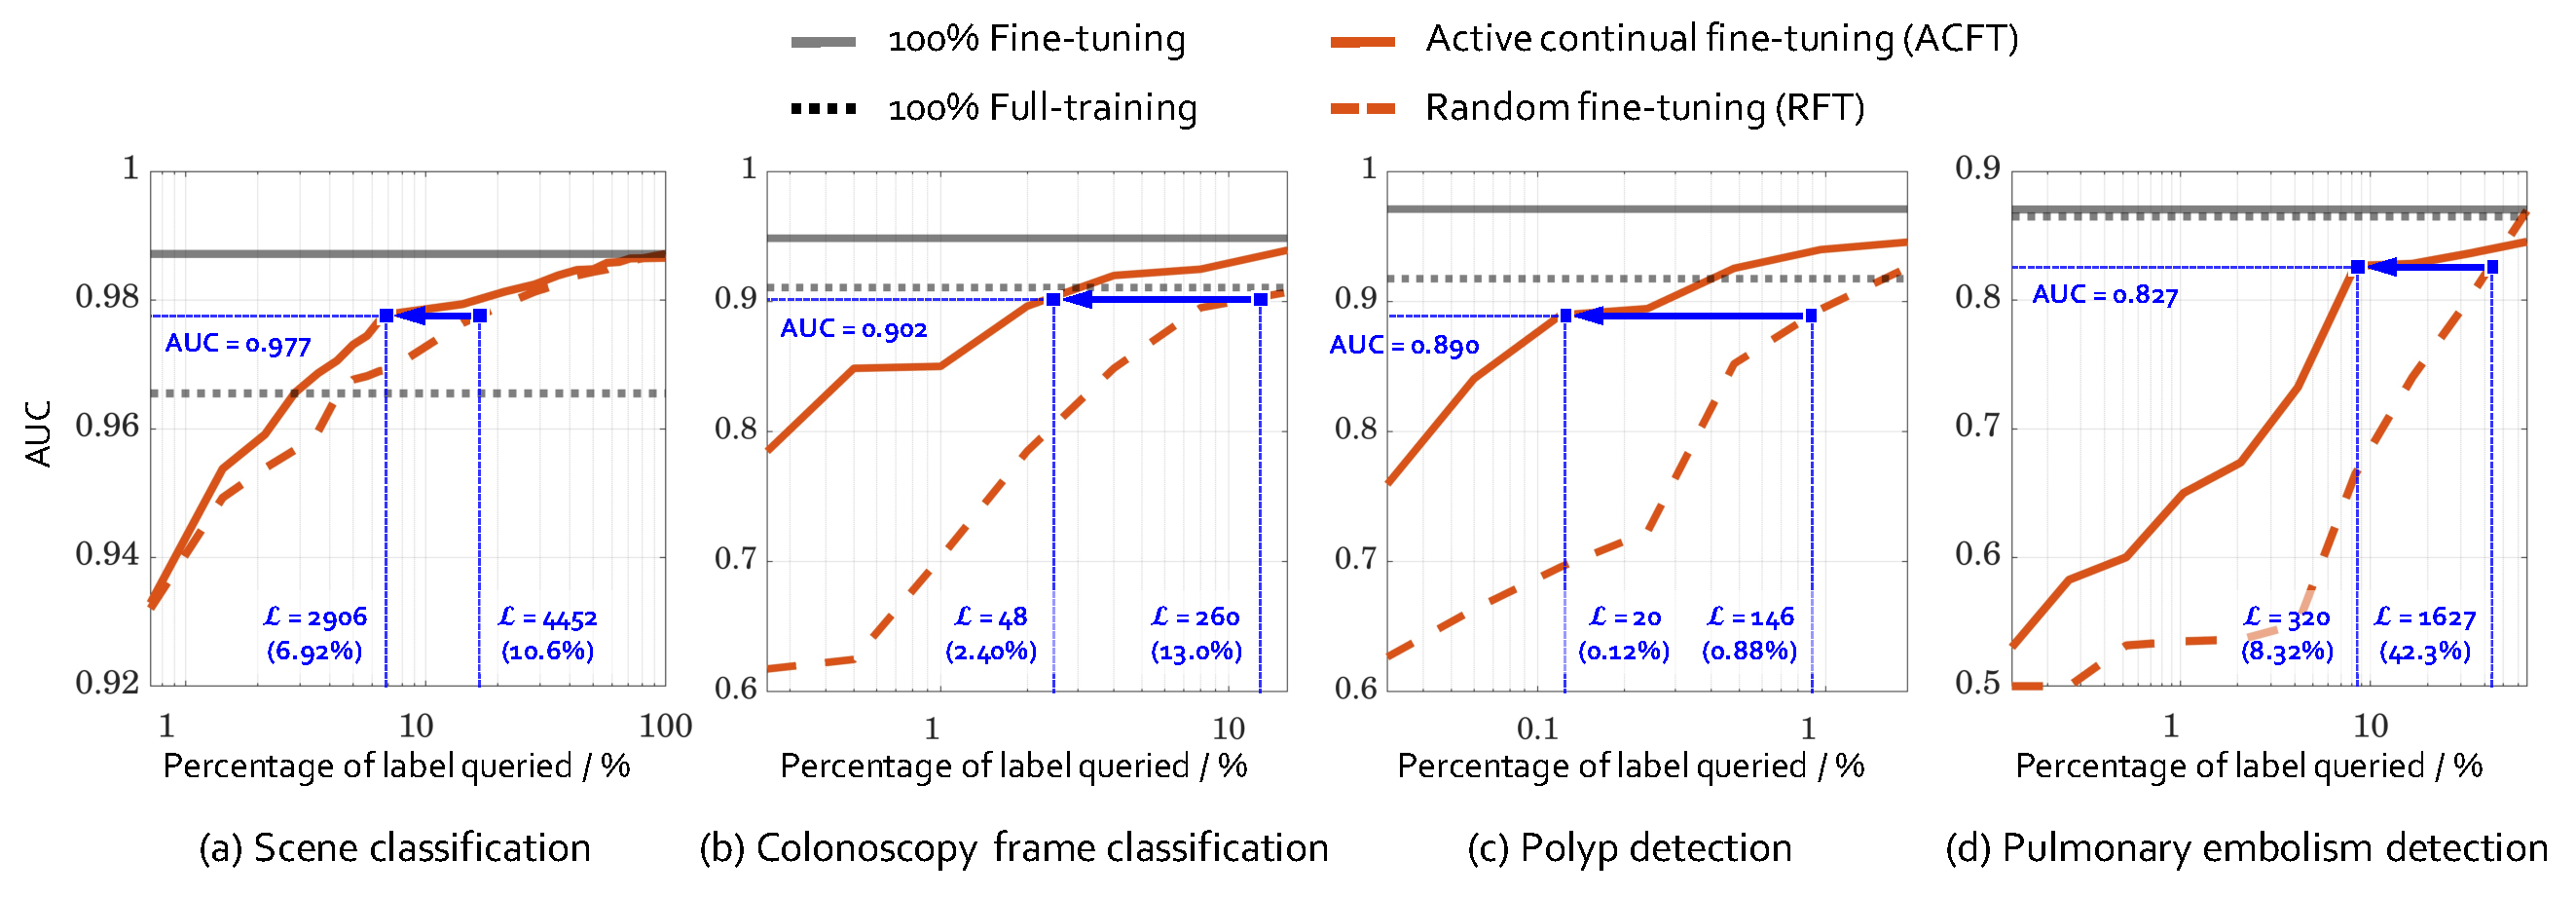
\includegraphics[width=0.95\columnwidth]{Figures/CH3/fig_result_highlights.pdf}
\end{center}
\caption[Active Continual Fine-tuning Reduces over 80\% Annotation Cost]{
ACFT aims to minimize the number of samples for experts to label by iteratively recommending the most informative and representative samples. For scene classification (a), by actively selecting 2,906 images (6.92\% of the entire dataset), ACFT can offer equivalent performance to the use of 4,452 images through random selection, thus saving 34.7\% annotation cost relative to random fine-tuning. Furthermore, with 1,176 actively-selected images (2.80\% of the whole dataset), ACFT can achieve performance equivalent to full training using 42,000 images, thereby saving 97.2\% annotation cost (relative to full training). 
In (b)---(d), we highlight the major results that compared with RFT, our ACFT can reduce the cost of annotation by 81.5\% for colonoscopy frame classification, 86.3\% for polyp detection, and 80.3\% for pulmonary embolism detection. 
% Following the standard active learning experimental setup, both ACFT and RFT select samples from the remaining training dataset; they will eventually use the same whole training dataset, naturally yielding similar performance at the end. However, the goal of active learning is to find such sweet spots where a learner can achieve an acceptable performance using the least number of labeled samples.
}
\label{ch3:fig:overall_result}
\end{sidewaysfigure}

% \fillandplacepagenumber
% \end{landscape}
%%%%%%%%%%%%%%%%%%%%%%%%%%%%%%%%%%%%%%%%%%%%







%%%%%%%%%%%%%%%%%%%%%%%%%%%%%%%%%%%%%%%%%%%%
\begin{algorithm}[t]
% \singlespace
\footnotesize
\caption{ACFT -- Active, Continual Fine-Tuning}
\label{ch3:alg:ACFT}
    \KwIn{\\
    \ \ \ $\mathcal{U}=\{\mathcal{C}_i\},$ $i\in [1,n]$ \{unlabeled pool $\mathcal{U}$\ contains $n$ candidates\}\\
    \ \ \ $\mathcal{C}_i=\{x_i^j\}$, $j\in [1,m]$ \{each $\mathcal{C}_i$ contains $m$ patches\}\\
    \ \ \ $M_0$: pre-trained CNN;
    \ $\alpha$: majority ratio;
    \ $b$: batch size;
    \ $\mathcal{Y}$: category set
    }
    \KwOut{\\
    \ \ \ $\mathcal{L}$: labeled candidates;
    \ $M_t$: fine-tuned CNN model at Step $t$
    }
    $\mathcal{L} \leftarrow \varnothing$;
    \ $t\leftarrow 1$\\
    \Repeat{ classification performance in a validation set plateaus}{

    \For{ each $\mathcal{C}_i \in \mathcal{U}$ }
    {
        $P_i \leftarrow M_{t-1}(\mathcal{C}_i)$ \{outputs of $M_{t-1}$ given $\forall x \in \mathcal{C}_i$\}\\
        $\mathcal{C}'_i \leftarrow \mathcal{C}_i$ descending sort on the predicted dominant class $\hat{\textbf{y}}_i$ by Eq.~\ref{eq:dominate_class} \\
        $\mathcal{C}^{\alpha}_i \leftarrow$ top $\alpha\times 100\%$ of the patches of the sorted list $\mathcal{C}'_i$ \\
        Compute $\textbf{\em a}_i$ for $\mathcal{C}^{\alpha}_i$ by Eq.~\protect\ref{eq:R}, \ie $\textbf{\em a}_i =\lambda_1 \textbf{\em e}_i+\lambda_2 \textbf{\em d}_i\quad$ \\
    }
    Sort $\mathcal{U}$ according to $\textbf{\em a}$ in descending order\\
    Compute sampling probability $\textbf{\em a}^{s}$ using sorted list $\textbf{\em a}'$ by Eq.~\ref{eq:randomness} \\
    Associate labels for $b$ candidates with sampling probabilities: $\mathcal{Q}\leftarrow Q(\textbf{\em a}^{s},b)$ \\
    $P \leftarrow M_{t-1}(\mathcal{L})$ \{outputs of $M_{t-1}$ given $\forall x \in \mathcal{L}$\} \\
    Select misclassified candidates from $\mathcal{L}$ based on their annotation: $\mathcal{H} \leftarrow J(P, \mathcal{L})$ \\
    Fine-tune $M_{t-1}$ with $\mathcal{H}\bigcup\mathcal{Q}$: $M_t \leftarrow F(\mathcal{H}\bigcup\mathcal{Q},M_{t-1})$  \\
    $\mathcal{L} \leftarrow  \mathcal{L}\bigcup \mathcal{Q};  \quad \mathcal{U} \leftarrow \mathcal{U} \setminus \mathcal{Q};  \quad t\leftarrow t+1$ \\
    }
\end{algorithm}
%%%%%%%%%%%%%%%%%%%%%%%%%%%%%%%%%%%%%%%%%%%%



\section{Approach \& Property}
\label{ch3:approach_property}



Active, continual fine-tuning (ACFT) was conceived in the context of computer-aided diagnosis (CAD) applied to medical imaging. A CAD system typically employs a candidate generator, which can quickly produce a set of candidates,  among which some are true positives and others are false positives. To train a classifier, each of the candidates must be labeled. In this work, an object to be labeled is considered as a ``candidate'' in general. We assume that each candidate takes one of $|\mathcal{Y}|$ possible labels.  To boost CNN performance for CAD systems, multiple patches are usually generated automatically for each candidate through data augmentation; those patches that are generated from the same candidate inherit the candidate's label. In other words, all labels are acquired at the candidate level. Mathematically, given a set of candidates, $\mathcal{U}=\{\mathcal{C}_1, \mathcal{C}_2, ..., \mathcal{C}_n\}$, where $n$ is the number of candidates, and each candidate $\mathcal{C}_i =\{x^{1}_i,x^{2}_i,...,x^{m}_i\}$ is associated with $m$ patches, our ACFT  algorithm iteratively selects a set of candidates for labeling as illustrated in~Alg.~\ref{ch3:alg:ACFT}.



\subsection{Selecting Based on Certainty and Consistency}
\label{ch3:approach_property:selection_certainty_consistency}

In active learning, the key is to develop criteria for determining ``worthiness'' of labeling a candidate. Our criteria for candidate ``worthiness'' are based on a simple, yet powerful, observation: all patches augmented from the same candidate share the same label; therefore, they are expected to have similar predictions by the current CNN. As a result, their {\em entropy} and {\em diversity} provide a useful indicator of the ``power'' of a candidate for elevating the performance of the current CNN. Intuitively, entropy captures classification certainty---a higher uncertainty value denotes a greater degree of information, whereas diversity indicates prediction consistency among the candidate patches---a higher diversity value denotes a greater degree of prediction inconsistency. Formally, assuming that each candidate takes one of $|\mathcal{Y}|$ possible labels, we define the entropy and diversity of $\mathcal{C}_i$ as

\begin{equation}
\label{eq:active_criteria}
\begin{split}
&\textbf{\em e}_i = -\frac{1}{m}\sum_{k=1}^{|\mathcal{Y}|}{\sum_{j=1}^{m}{P_i^{j,k}\log{P_i^{j,k}}}}, \\
&\textbf{\em d}_i = \sum_{k=1}^{|\mathcal{Y}|}{\sum_{j=1}^m{\sum_{l=j}^m{(P_i^{j,k}-P_i^{l,k})\log{\frac{P_i^{j,k}}{P_i^{l,k}}}}}}
\end{split}
\end{equation}
Combining entropy and diversity yields
\begin{equation}
\label{eq:R}
\textbf{\em a}_i =\lambda_1 \textbf{\em e}_i+\lambda_2 \textbf{\em d}_i
\end{equation}
where $\lambda_1$ and $\lambda_2$ are trade-offs between entropy and diversity. We use two parameters for convenience,  to easily turn on/off entropy or diversity during experiments.




\subsection{Handling Noisy Labels via Majority Selection}
\label{ch3:approach_property:handling_noisy_labels_majority_selection}

Automatic data augmentation is essential for boosting CNN performance, but it inevitably generates ``hard'' samples for some candidates, as shown in \figurename~\ref{ap1:fig:dataset_annotation}(c), injecting noisy labels. Therefore, to significantly enhance the robustness of our method, we compute entropy and diversity by selecting only a portion of the patches of each candidate according to the predictions by the current CNN.

Specifically, for each candidate $\mathcal{C}_i$ we first determine its dominant category, which is defined by the category with the highest confidence in the mean prediction. That is,
\begin{equation}
\label{eq:dominate_class}
\hat{\textbf{y}}_i =  \argmax_{y \in \mathcal{Y}} \frac{1}{m}\sum_{j=1}^{m}P^{j,y}_i
\end{equation}
where $P^{j,y}_i$ is the output of each patch $j$ from the current CNN given $\forall x \in \mathcal{C}_i$ on label $y$. After sorting $P_i$ according to dominant category $\hat{\textbf{y}}_i$, we apply Eq.~\ref{eq:R} to top $\alpha\times$100\% of the patches to construct the score matrix $\textbf{\em a}_i$ of size $\alpha m \times \alpha m$ for each candidate $\mathcal{C}_i$ in $\mathcal{U}$. Our proposed majority selection method automatically excludes those patches with noisy labels owning to their high consistency in the majority of predictions.

%%%%%%%%%%%%%%%%%%%%%%%%%%%%%%%%%%%%%%%%%%%%
% \begin{landscape}
% \thispagestyle{empty}

\begin{sidewaysfigure}
\begin{center}
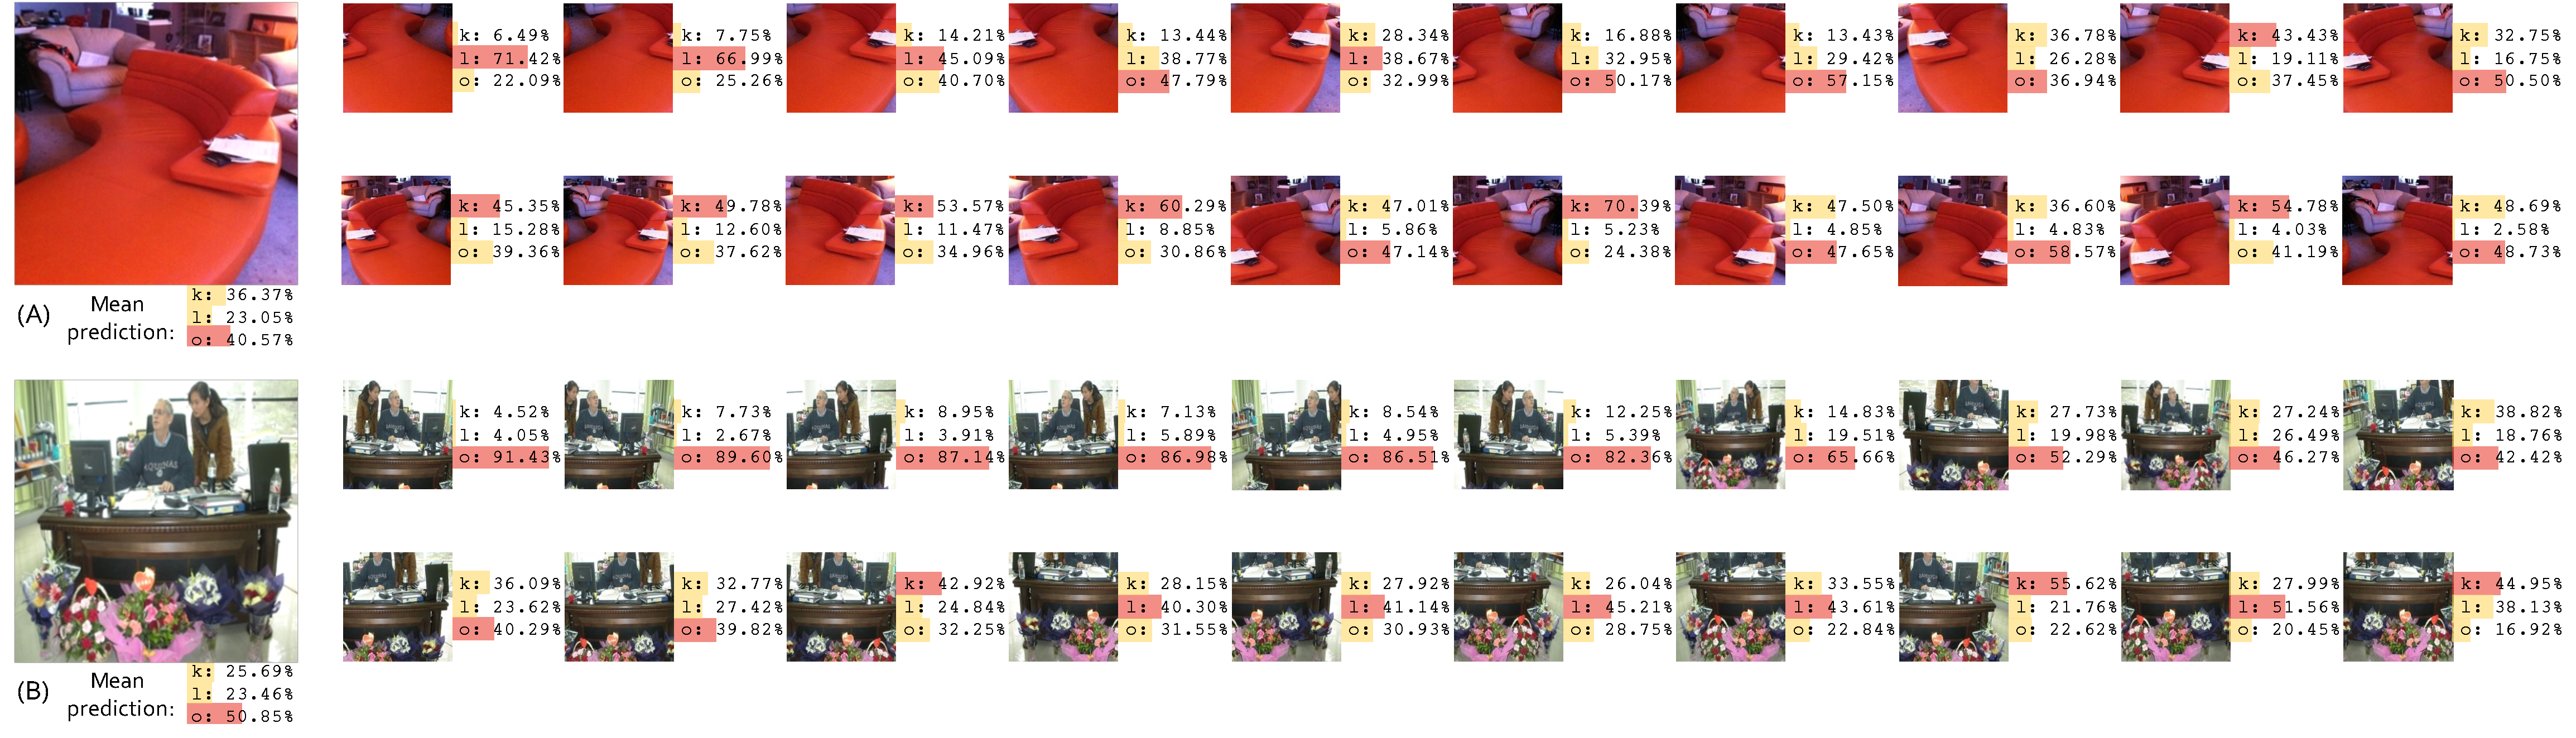
\includegraphics[width=1.0\columnwidth]{Figures/CH3/fig_data_augumentation.pdf}
\end{center}
\caption[The Significance of Majority Selection]{
% Automatic data augmentation inevitably generates noisy patches, and there is no need to classify all patches confidently. 
% Therefore, we propose majority selection, which computes active selection criteria on only the top 25\% of the patches with the highest confidences on the dominant predicted category.
To demonstrate the necessity of majority selection, we illustrate two images (A and B) and their augmented patches, arranged according to the dominant category predicted by the CNN. 
Based on \textsc{Places-3}, Image A is labeled as {\em living room}, and its augmented patches are mostly incorrectly classified by the current CNN; therefore, including it in the training set is of great value. On the contrary, Image B is labeled as {\em office}, and the current CNN classifies most of its augmented patches as {\em office} with high confidence; labeling it would be of limited utility. 
Without majority selection, the criteria would mislead the selection, as it indicates that Image B is more diverse than Image A (297.52 vs. 262.39) while sharing similar entropy (17.33 vs. 18.50). With majority selection, the criteria show that Image A is considerably more uncertain and diverse than Image B, measured by either entropy (4.59 vs. 2.17) or diversity (9.32 vs. 0.35), and as expected, more worthy of labeling. From this active selection analysis, we remark that the majority selection is a critical component in our ACFT.
}
\label{ch3:fig:places_examples}
\end{sidewaysfigure}

% \fillandplacepagenumber
% \end{landscape}
%%%%%%%%%%%%%%%%%%%%%%%%%%%%%%%%%%%%%%%%%%%%



\subsection{Injecting Randomization into Active Selection}
\label{ch3:approach_property:injecting_randomization_active_selection}

As discussed in~\citet{borisov2010active} and~\citet{zhou2017fine}, simple random selection may outperform active selection at the beginning, because the active selection method depends on the current model selecting examples for labeling. As a result, a poor selection made at an early stage may adversely affect the quality of subsequent selections, whereas the random selection approach is less frequently locked into a poor hypothesis. In other words, the active selection method concentrates on exploiting the knowledge gained from the labels already acquired to further explore the decision boundary, whereas the random selection approach concentrates solely on exploration, and is thereby able to locate areas of the feature space where the classifier performs poorly. Therefore, an effective active learning strategy must strike a balance between exploration and exploitation.
Towards this end, we inject randomization into our method by selecting actively according to the sampling probability $\textbf{\em a}^{s}_i$.

\begin{equation}
\label{eq:randomness}
\begin{split}
\textbf{\em a}'_i=(\textbf{\em a}'_i-\textbf{\em a}'_{\omega b})/(\textbf{\em a}'_1-\textbf{\em a}'_{\omega b}), \\
 \textbf{\em a}^{s}_i=\textbf{\em a}'_i/\sum_i{\textbf{\em a}'_i},\quad \forall i \in [1,\omega b]
\end{split}
\end{equation}
where $\textbf{\em a}'_i$ is sorted $\textbf{\em a}_i$ according to its value in descending order, and $\omega$ is named random extension.
Suppose $b$ number of candidates are required for annotation. Instead of selecting top $b$ candidates, we extend the candidate selection pool to $\omega b$. Then we select candidates from this pool with their sampling probabilities $\textbf{\em a}^{s}_i$ to inject randomization.


\subsection{Five Unique Properties}
\label{ch3:approach_property:several_unique_properties}


\begin{enumerate}[noitemsep]

    \item \textit{ACFT integrates entropy and diversity.} Our algorithm actively selects the most uncertain and informative candidates by naturally exploiting expected consistency among the patches within each candidate, reducing the number of redundancy and outliers. 
    
    \item \textit{ACFT overcomes noisy labels associated with augmentation.} Our algorithm computes selection criteria locally on a small number of patches within each candidate, saving considerable computation cost for diversity metric.
    
    \item \textit{ACFT tackles cold start problem by injecting randomness.} Our algorithm balances exploration and exploitation by incorporating randomness into active selection, demonstrating the superior performance even at the beginning of active learning procedure.
    
    \item \textit{ACFT balances training samples among classes.} Our algorithm seeks the most critical candidates to be annotated for the current model, ensuring a comparable number of candidates selected from minority classes and preventing the model from being skewed towards majority classes.
    
    \item \textit{ACFT is generic and applicable to many imaging tasks.} Our algorithm was initially developed for the purpose of medical imaging, but it also demonstrates over 30\% annotation reduction for the scene classification task in natural imaging as well. We illustrate the ideas behind ACFT with the \textsc{Places-3} dataset~\citep{zhou2017places}, where no candidate generator is needed, as each image may be directly regarded as a candidate. 

\end{enumerate}



\section{Experiment \& Result}
\label{ch3:experiment_result}

In this section, \figurename~\ref{ch3:fig:overall_result} begins with an overall performance between our active continual fine-tuning (ACFT) and random fine-tuning (RFT), revealing the amount of annotation effort that has been reduced in each application. \figurename~\ref{ch3:fig:selection_approaches_comparison_alexnet} and \figurename~\ref{ch3:fig:selection_approaches_comparison_googlenet} compare eight different active selecting criteria, demonstrating that majority selection and randomness are critical in finding the most representative samples to elevate the current CNN's performance.
\figurename~\ref{ch3:fig:predicted_distribution} further presents the observed distribution of each active selecting criteria, qualitatively confirming the rationale of our devised candidate selecting approaches.
\tableautorefname~\ref{ch3:tab:main_results} finally compares four different active learning strategies, suggesting that continual fine-tuning using newly annotated candidates enlarged by those misclassified candidates significantly saves computational resources while maintaining the compelling performance in all three medical applications.

%%%%%%%%%%%%%%%%%%%%%%%%%%%%%%%%%%%%%%%%%%%%
\begin{table}[t]
\begin{center}
\begin{threeparttable}
\footnotesize
\caption[Abbreviation and Definition of Learning Strategies]{
Active learning strategy definition. We have codified different learning strategies covering the makeup of training samples and the initial model weights of fine-tuning.}
\label{ch3:tab:terminology}
    \begin{tabular}{p{0.15\textwidth}p{0.8\textwidth}}
    \hline
    \textbf{Code} & \textbf{Description of learning strategy} \\
    \hline
    RFT$_{(LQ)}$ & Fine-tuning from $M_{0}$ using $\mathcal{L}$ and randomly selected $\mathcal{Q}$ \\
    AFT$_{(LQ)}$ & Fine-tuning from $M_0$ using $\mathcal{L}$ and actively selected $\mathcal{Q}$ \\
    ACFT$_{(Q)}$ & Continual fine-tuning from $M_{t-1}$ using actively selected $\mathcal{Q}$ only \\
    ACFT$_{(LQ)}$ & Continual fine-tuning from $M_{t-1}$ using $\mathcal{L}$ and actively selected $\mathcal{Q}$ \\
    ACFT$_{(HQ)}$ & Continual fine-tuning from $M_{t-1}$ using $\mathcal{H}$ and actively selected $\mathcal{Q}$ \\
    \hline
    \end{tabular}
    \begin{tablenotes}
        \footnotesize
        \item[1] $\mathcal{L}$: Labeled candidates.
        \item[2] $\mathcal{Q}$: Newly annotated candidates.
        \item[3] $\mathcal{H}$: Misclassified candidates.
        \item[4] $M_0$: Pre-trained CNNs from large scale dataset (like \textsc{ImageNet}).
        \item[5] $M_{t-1}$: Pre-trained CNNs from last active selecting iteration.
    \end{tablenotes}
\end{threeparttable}
\end{center}
\end{table}
%%%%%%%%%%%%%%%%%%%%%%%%%%%%%%%%%%%%%%%%%%%%


%%%%%%%%%%%%%%%%%%%%%%%%%%%%%%%%%%%%%%%%%%%%
\begin{table}[t]
\caption[Analysis on Active Selection Pattern]{
Active selection patterns analysis. We illustrate the relationships among seven prediction patterns and four active selection criteria, assuming that a candidate $\mathcal{C}_i$ has 11 augmented patches, and their probabilities $P_i$ are predicted by the current CNN, presented in the second column. With majority selection, the entropy and diversity are calculated based on the top 25\% (3 patches in this illustration) highest confidences on the dominant predicted category. The first choice of each method (column) is \textbf{bolded} and the second choice is \underline{underlined}.
}
\label{ch3:tab:predict_pattern}
\begin{center}
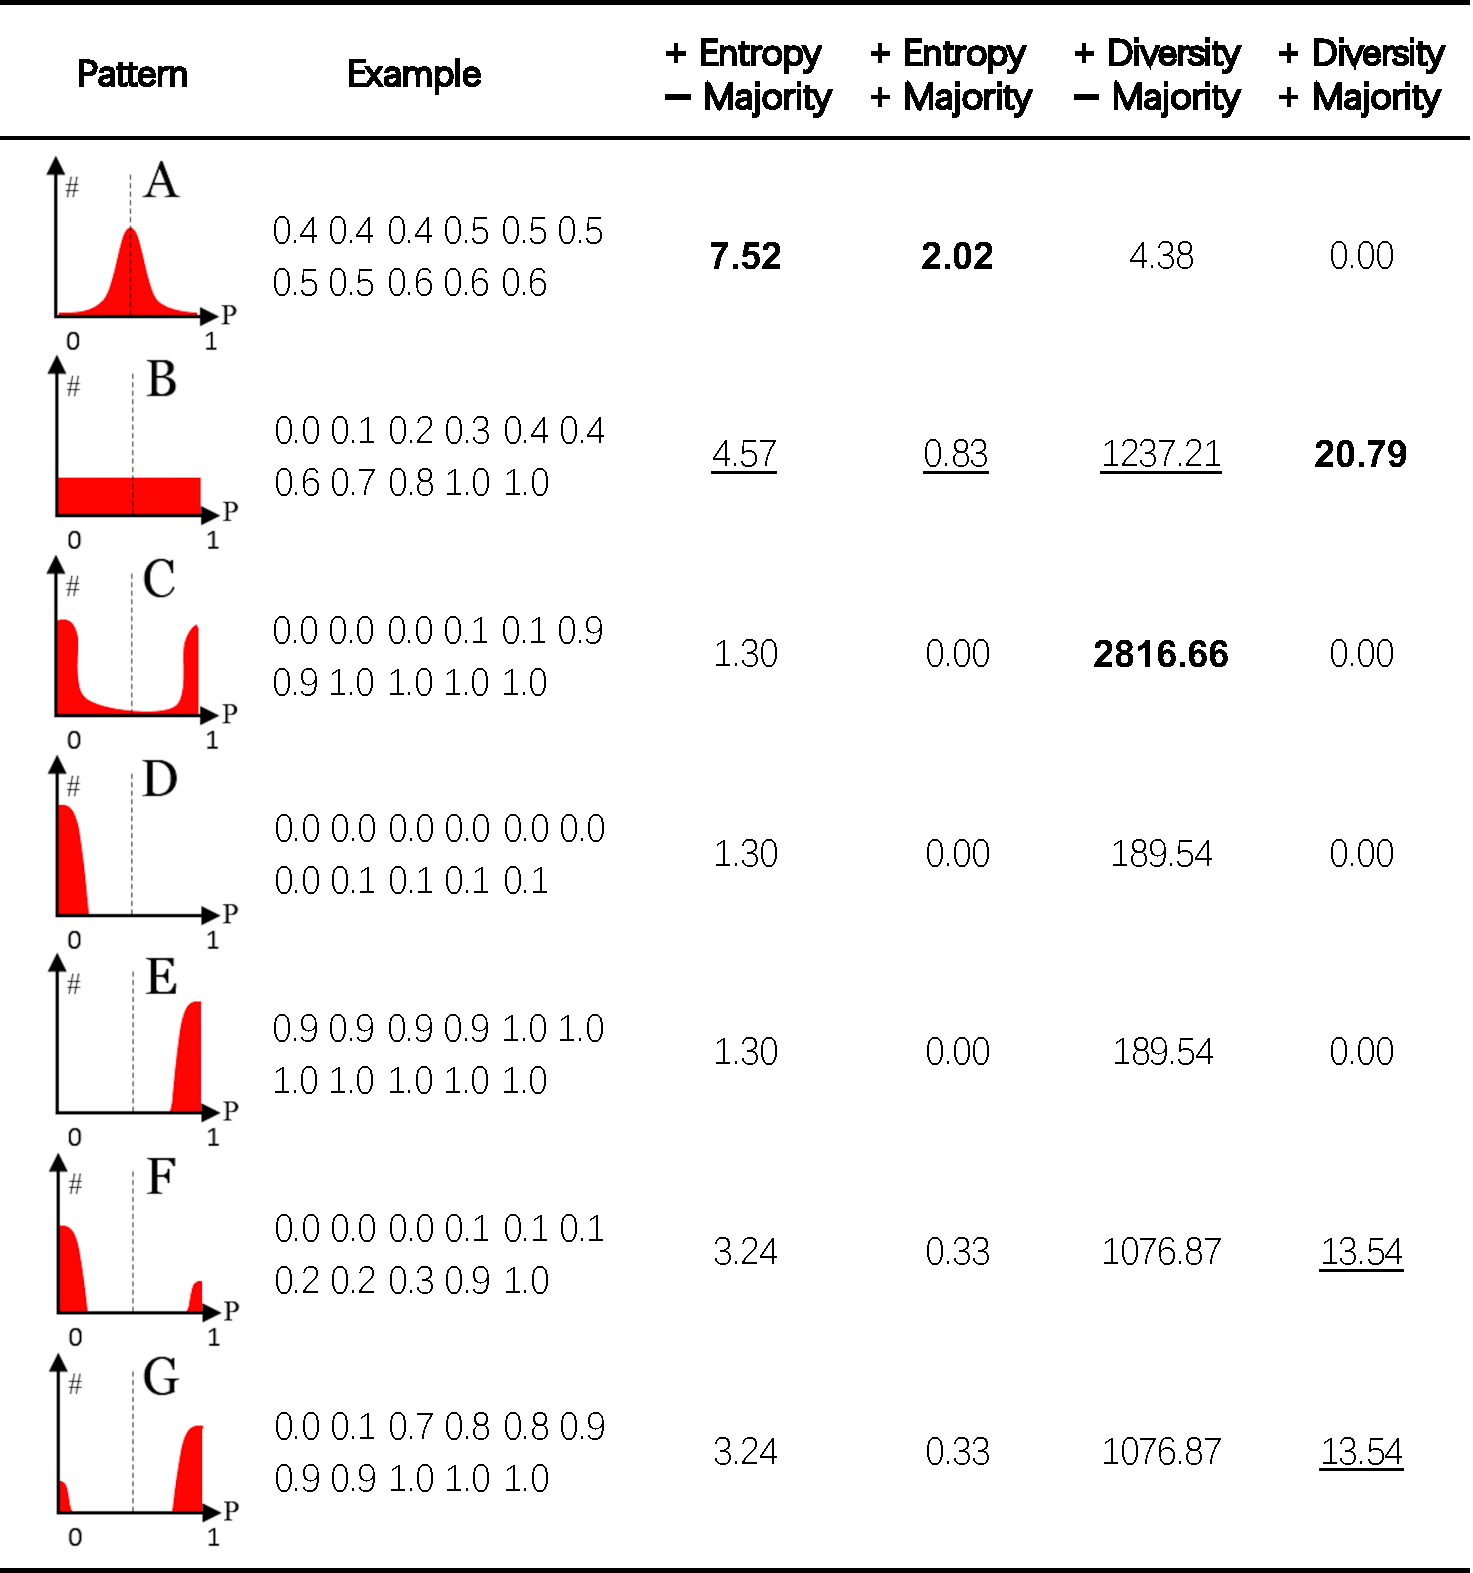
\includegraphics[width=0.7\linewidth]{Figures/CH3/fig_hypothsis_pattern.pdf}\\
\end{center}
\end{table}
%%%%%%%%%%%%%%%%%%%%%%%%%%%%%%%%%%%%%%%%%%%%

\subsection{Benchmarking Active, Continual Fine-Tuning}
\label{sch2:experiment_result:benchmarking_active_continual_finetuning}


\citet{tajbakhsh2016convolutional} reported the state-of-the-art performance of fine-tuning and learning from scratch using entire datasets, which are used to establish baseline performance for comparison. These authors also investigated the performance of (partial) fine-tuning using a sequence of partial training datasets, but our dataset partitions are different from theirs. Therefore, for a fair comparison with their approach, we introduce RFT, which fine-tunes the original model $M_0$  from the beginning, using all available labeled samples $\mathcal{L}\bigcup\mathcal{Q}$, where $\mathcal{Q}$ is randomly selected at each step. 

We summarized several active learning strategies in \tableautorefname~\ref{ch3:tab:terminology}. Studying different active learning strategies is important because active learning procedure can be very computationally inefficient in practice, in terms of label reuse and model reuse. We present two strategies that aim at overcoming the above limitations. First, we propose to combine newly annotated data with the labeled data that is misclassified by the current CNN. Second, we propose continual fine-tuning to speed up model training and, in turn, encourage data reuse.
ACFT$_{(HQ)}$ denotes the optimized learning strategy, which continually fine-tunes the current model $M_{t-1}$ using newly annotated candidates enlarged by those misclassified candidates; that is, $\mathcal{Q}\bigcup\mathcal{H}$. 
Compared with other learning strategy baselines~\citep{tajbakhsh2016convolutional, zhou2017fine,zhou2019integrating} as codified in \tableautorefname~\ref{ch3:tab:terminology}, ACFT$_{(HQ)}$ saves training time through faster convergence compared with repeatedly fine-tuning the original pre-trained CNN, and boosts performance by eliminating easy samples, focusing on hard samples, and preventing catastrophic forgetting. In all three applications, our ACFT begins with an empty training dataset and directly uses pre-trained models (AlexNet and GoogLeNet) on ImageNet.


\subsection{Assessing Eight Active Selecting Criteria}
\label{ch3:experiment_result:assessing_eight_active_selecting_criteria}

We meticulously monitored the active selection process and examined the selected candidates. For example, we include the top ten candidates selected by the four ACFT methods at Step 3 in colonoscopy frame classification in \figurename~\ref{ch3:fig:predicted_distribution}. From this process, we have observed the following:
\begin{itemize}
\item Patterns A and B are dominant in the earlier stages of ACFT as the CNN has not been fine-tuned properly to the target domain;
\item Patterns C, D and E are dominant in the later stages of ACFT as the CNN has been largely fine-tuned on the target dataset;
\item Majority selection is effective for excluding Patterns C, D, and E, whereas entropy only (without the majority selection) can handle Patterns C, D, and E reasonably well;
\item Patterns B, F, and G generally make good contributions to elevating the current CNN's performance;
\item Entropy and entropy+majority favor Pattern A due to its higher degree of uncertainty, and;
\item Diversity+majority prefers Pattern B whereas diversity prefers Pattern C. This is why diversity may cause sudden disturbances in the CNN's performance and why diversity+majority is generally preferred.

\end{itemize}

%%%%%%%%%%%%%%%%%%%%%%%%%%%%%%%%%%%%%%%%%%%%
% \begin{landscape}
% \thispagestyle{empty}

% \begin{figure}[t]
\begin{sidewaysfigure}
\begin{center}
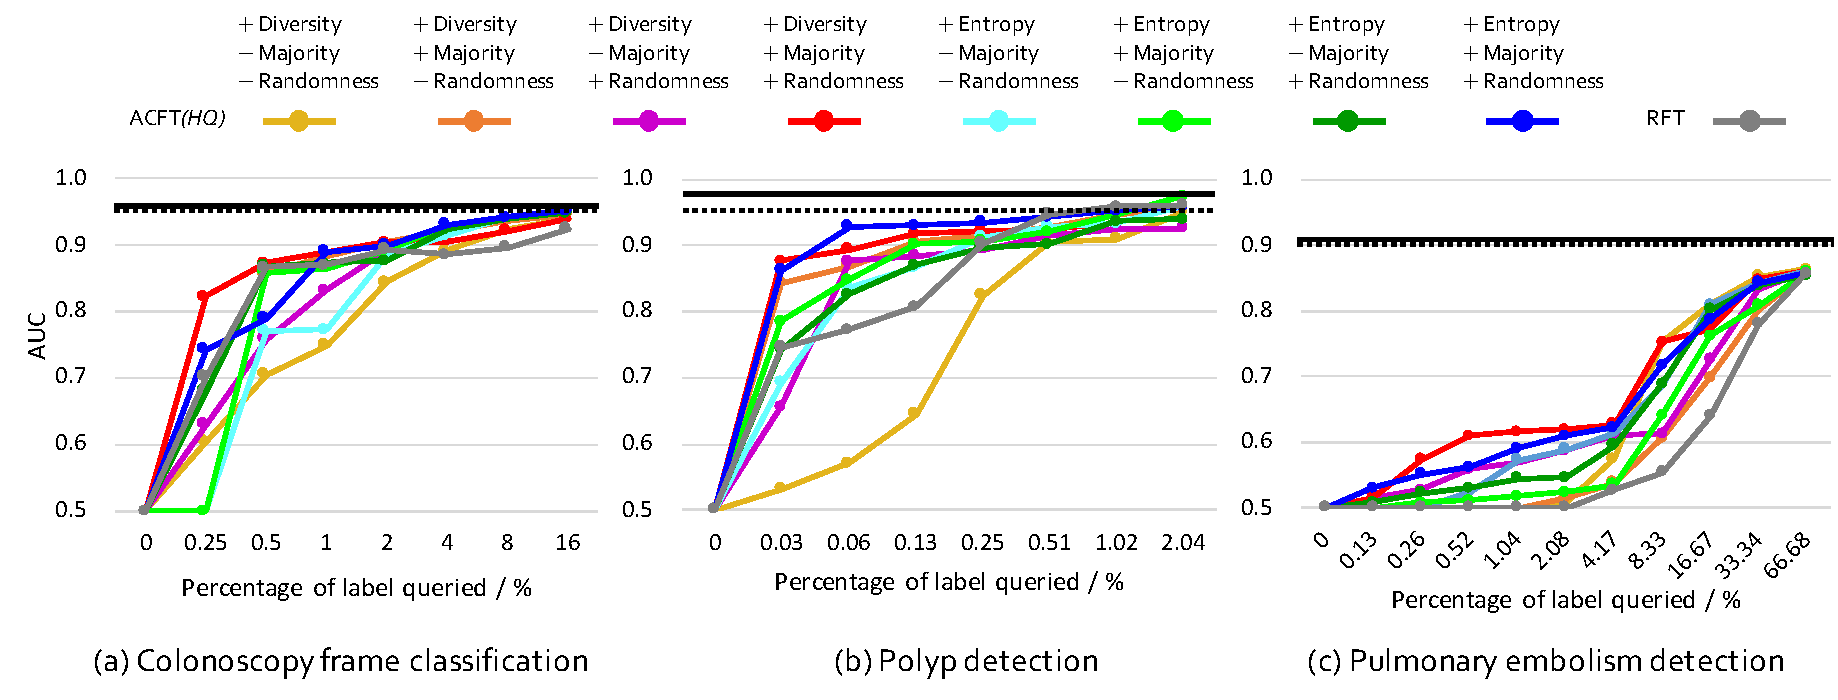
\includegraphics[width=1.0\columnwidth]{Figures/CH3/fig_selection_approaches_comparison_alexnet.pdf}
\end{center}
\caption[Assessment of Eight Active Selecting Criteria (AlexNet)]{
Comparing eight active selection approaches with random selection on AlexNet~\citep{krizhevsky2012imagenet} for our three distinct medical applications, including (a) colonoscopy frame classification, (b) polyp detection, and (c) pulmonary embolism detection, demonstrates consistent patterns with AlexNet. The solid black line denotes the current state-of-the-art performance of fine-tuning using full training data and the dashed black line denotes the performance of training from scratch using full training data.}
\label{ch3:fig:selection_approaches_comparison_alexnet}
\end{sidewaysfigure}
% \end{figure}

% \fillandplacepagenumber
% \end{landscape}
%%%%%%%%%%%%%%%%%%%%%%%%%%%%%%%%%%%%%%%%%%%%

%%%%%%%%%%%%%%%%%%%%%%%%%%%%%%%%%%%%%%%%%%%%
% \begin{landscape}
% \thispagestyle{empty}

\begin{sidewaysfigure}
\begin{center}
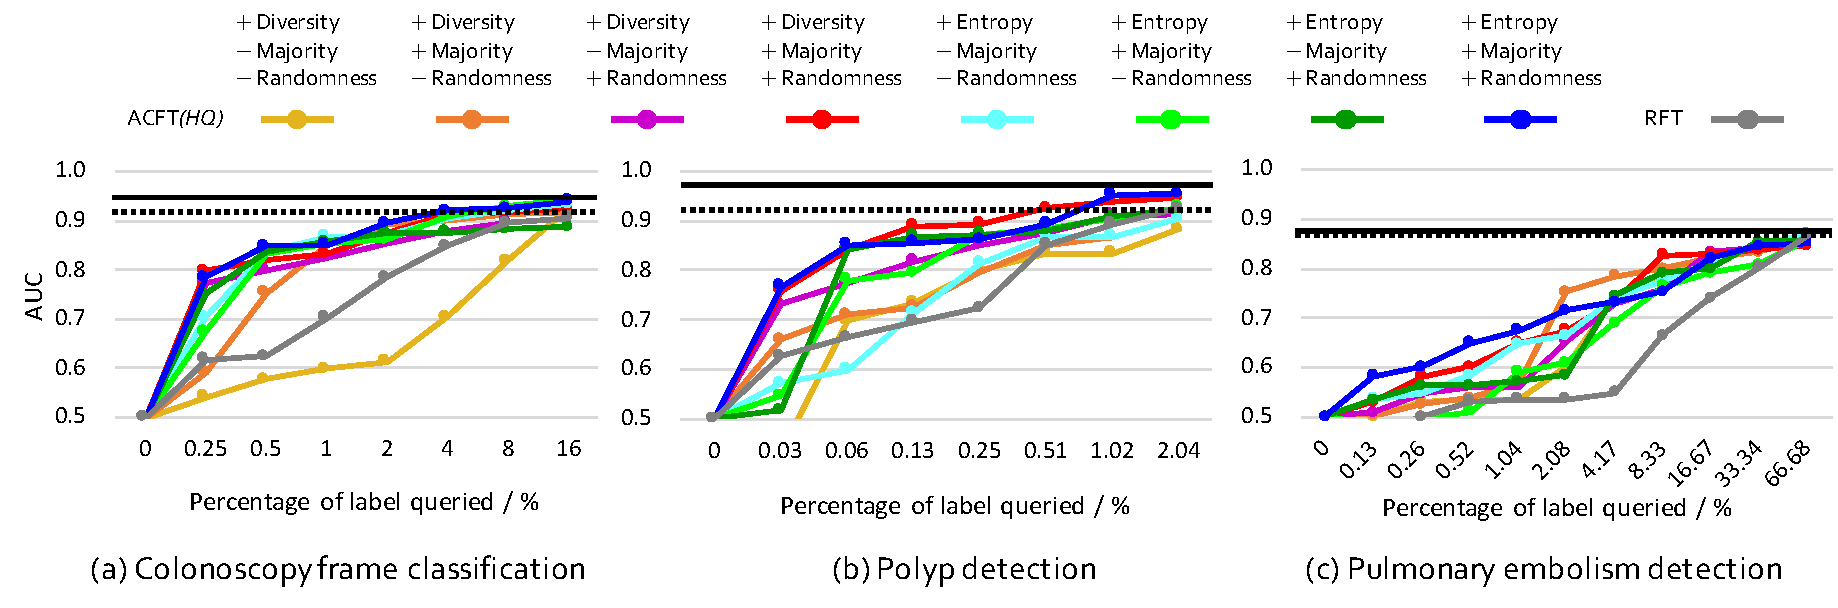
\includegraphics[width=1.0\columnwidth]{Figures/CH3/fig_selection_approaches_comparison_googlenet.pdf}
\end{center}
\caption[Assessment of Eight Active Selecting Criteria (GoogleNet)]{
Comparing eight active selection approaches with random selection on GoogLeNet~\citep{szegedy2015going} for our three distinct medical applications, including (a) colonoscopy frame classification, (b) polyp detection, and (c) pulmonary embolism detection, demonstrates consistent patterns with AlexNet. The solid black line denotes the current state-of-the-art performance of fine-tuning using full training data and the dashed black line denotes the performance of training from scratch using full training data.}
\label{ch3:fig:selection_approaches_comparison_googlenet}
\end{sidewaysfigure}

% \fillandplacepagenumber
% \end{landscape}
%%%%%%%%%%%%%%%%%%%%%%%%%%%%%%%%%%%%%%%%%%%%

%%%%%%%%%%%%%%%%%%%%%%%%%%%%%%%%%%%%%%%%%%%%
% \begin{landscape}
% \thispagestyle{empty}

% \begin{threeparttable}[t]
\begin{sidewaystable}
\scriptsize
\begin{center}
    \caption[Comparison of Learning Strategies and Selecting Criteria]{
    Comparison of proposed active learning strategies and selection criteria. As measured by the Area under the Learning Curve (ALC), bolded values in the table indicate the outstanding learning strategies (see \tableautorefname~\ref{ch3:tab:terminology}) using certain active selection criteria, and starred values represent the best performance taking both learning strategies and active selection criteria into consideration. For all three applications, we report baseline performance of random fine-tuning (RFT) using AlexNet in the table footnote. Considering the variance of random sampling for each active learning step, we conduct five independent trials for RFT and report the mean and standard deviation (mean$\pm$s.d.).}
    \label{ch3:tab:main_results}
    \begin{tabular}{p{0.1\textwidth}p{0.14\textwidth}|p{0.07\textwidth}p{0.07\textwidth}p{0.07\textwidth}p{0.07\textwidth}|p{0.07\textwidth}p{0.07\textwidth}p{0.07\textwidth}p{0.07\textwidth}}
    \hline
    Application & Learning strategy & $+$ Diversity\newline $-$ Majority\newline $-$ Random & $+$ Diversity\newline $+$ Majority\newline $-$ Random & $+$ Diversity\newline $-$ Majority\newline $+$ Random & $+$ Diversity\newline $+$ Majority\newline $+$ Random & $+$ Entropy\newline $-$ Majority\newline $-$ Random & $+$ Entropy\newline $+$ Majority\newline $-$ Random & $+$ Entropy\newline $-$ Majority\newline $+$ Random & $+$ Entropy\newline $+$ Majority\newline $+$ Random \\
    \hline
    \multirow{4}{*}{\tabincell{l}{Colonoscopy\\frame\\classification}} & ACFT$_{(Q)}$ & 0.8375 & 0.8773 & 0.8995 & 0.9160 & 0.8444 & 0.8227 & 0.9136 & 0.9061\\
    & ACFT$_{(LQ)}$ & 0.8501 & 0.8956 & 0.9083 & 0.9262 & 0.9149 & 0.9051 & 0.9033 & 0.9223\\
    & AFT$_{(LQ)}$ & \textbf{0.9183} & \textbf{0.9253} & \textbf{0.9299} & \textbf{0.9344}$^\star$ & \textbf{0.9219} & 0.9180 & \textbf{0.9268} & 0.9291\\
    & ACFT$_{(HQ)}$ & 0.9048 & 0.9236 & 0.9241 & 0.9179 & 0.9198 & \textbf{0.9266} & 0.9257 & \textbf{0.9293}\\
    \hline
    \multirow{4}{*}{\tabincell{l}{Polyp\\detection}} & ACFT$_{(Q)}$ & 0.8669 & 0.9023 & 0.8984 & 0.9168 & 0.8834 & 0.8656 & 0.9034 & 0.9271\\
    & ACFT$_{(LQ)}$ & 0.9195 & 0.9142 & \textbf{0.9497} & \textbf{0.9488} & 0.9204 & 0.9255 & \textbf{0.9475} & 0.9444\\
    & AFT$_{(LQ)}$ & \textbf{0.9242} & 0.9285 & 0.9353 & 0.9355 & 0.9292 & 0.9238 & 0.9367 & \textbf{0.9522}$^\star$ \\
    & ACFT$_{(HQ)}$ & 0.9013 & \textbf{0.9370} & 0.9116 & 0.9363 & \textbf{0.9321} & \textbf{0.9436} & 0.9196 & 0.9443\\
    \hline
    \multirow{4}{*}{\tabincell{l}{Pulmonary\\embolism\\detection}} & ACFT$_{(Q)}$ & 0.7828 & 0.7911 & 0.7690 & 0.7977 & 0.7855 & 0.7736 & 0.7296 & 0.7833\\
    & ACFT$_{(LQ)}$ & 0.8083 & \textbf{0.8176} & 0.7975 & \textbf{0.8263} & 0.8032 & \textbf{0.8086} & 0.8022 & \textbf{0.8245}\\
    & AFT$_{(LQ)}$ & 0.7650 & 0.7973 & 0.7978 & 0.8040 & 0.7917 & 0.7878 & 0.7964 & 0.8222\\
    & ACFT$_{(HQ)}$ & \textbf{0.8272}$^\star$ & 0.7876 & \textbf{0.8047} & 0.8245 & \textbf{0.8218} & 0.7995 & \textbf{0.8155} & 0.8205\\
    \hline
    \end{tabular}
    \begin{tablenotes}
        \scriptsize
        \item[1] RFT in colonoscopy frame classification: ALC = 0.8958$\pm$0.0176
        \item[2] RFT in polyp detection: ALC = 0.9358$\pm$0.0130
        \item[3] RFT in pulmonary embolism detection: ALC = 0.7849$\pm$0.0261
    \end{tablenotes}
\end{center}
\end{sidewaystable}
% \end{threeparttable}
% % }
% \fillandplacepagenumber
% \end{landscape}
%%%%%%%%%%%%%%%%%%%%%%%%%%%%%%%%%%%%%%%%%%%%

\subsection{Comparing Four Active Learning Strategies}
\label{ch3:experiment_result:comparing_four_active_learning_strategies}

As summarized in \tableautorefname~\ref{ch3:tab:terminology}, several active learning strategies can be derived. The prediction performance was evaluated according to the Area under the Learning Curve (ALC), in which the learning curve plots AUC as a function of the number of labels queried~\citep{guyon2011results}, computed on the testing dataset. \tableautorefname~\ref{ch3:tab:main_results} shows the ALC of ACFT$_{(Q)}$, ACFT$_{(LQ)}$, AFT$_{(LQ)}$ and ACFT$_{(HQ)}$ compared with RFT. Our comprehensive experiments have demonstrated that:

\begin{itemize}
    \item ACFT$_{(Q)}$ considers only newly selected candidates for fine-tuning, resulting in an unstable CNN performance due to the catastrophic forgetting of the previous samples;
    \item ACFT$_{(LQ)}$ requires a careful parameter adjustment. Although its performance is acceptable, it requires the same computing time as AFT$_{(LQ)}$, indicating that there is no advantage to continually fine-tuning the current model;
    \item AFT$_{(LQ)}$ shows the most reliable performance compared with ACFT$_{(Q)}$ and ACFT$_{(LQ)}$;
    \item The optimized version, ACFT$_{(HQ)}$, shows comparable performance to AFT$_{(LQ)}$ and occasionally outperforms AFT$_{(LQ)}$ by eliminating easy samples, focusing on hard samples, and preventing catastrophic forgetting.
\end{itemize}

In summary, our results suggest that (1) it is unnecessary to re-train models repeatedly from scratch for each active learning step and (2) learning newly annotated candidates plus a small portion of the misclassified candidates leads to equivalent performance to using the entire labeled set.


\subsection{Cutting $>$80\% Annotation Cost for Medical Applications}
\label{ch3:experiment_result:cutting_annotation_cost}


\textit{ACFT reduces 82\% annotation cost in quality assessment.} \figurename~\ref{ch3:fig:overall_result}(b) shows that ACFT, with approximately 120 candidate queries (6\%), achieves performance equivalent to a 100\% trained dataset fine-tuned from AlexNet (solid black line, AUC = 0.9366), and, with only 80 candidate queries (4\%), can achieve performance equivalent to a 100\% training dataset learned from scratch (dashed black line, AUC = 0.9204). Using only 48 candidate queries, ACFT equals the performance of RFT at 260 candidate queries. Therefore, about 81.5\% of the labeling cost associated with with RFT in colonoscopy frame classification is recovered using ACFT. Detailed analysis in \figurename~\ref{ch3:fig:selection_approaches_comparison_alexnet} and \figurename~\ref{ch3:fig:selection_approaches_comparison_googlenet} reveals that during the early stages, RFT yields performance superior to some of the active selecting processes because: 
1) random selection gives samples with the positive-negative ratio compatible with the testing and validation dataset; 2) the pre-trained model gives poor predictions in the domain of medical imaging, as it was trained by natural images. Its output probabilities are mostly inconclusive or even opposite, yielding poor selection scores. However, with randomness injected, as described in Sec.~\ref{ch3:approach_property:injecting_randomization_active_selection}, ACFT (+majority and +randomness) shows superior performance, even at early stages, with continued performance improvement during subsequent steps (see the red and blue curves in \figurename~\ref{ch3:fig:selection_approaches_comparison_alexnet} and \figurename~\ref{ch3:fig:selection_approaches_comparison_googlenet}). Besides, evidenced by \tableautorefname~\ref{ch3:tab:main_results}, ACFT performs comparably with AFT, but, unlike the latter, does not require use of the entire labeled dataset or fine-tuning from the beginning. 

\textit{ACFT reduces 86\% annotation cost in polyp detection.} \figurename~\ref{ch3:fig:overall_result}(c) shows that ACFT, with approximately 320 candidate queries (2.04\%), can achieve performance equivalent to a 100\% training dataset fine-tuned from AlexNet (solid black line, AUC = 0.9615), and, with only 10 candidate queries (0.06\%), can achieve  performance equivalent to a 100\% training dataset learned from scratch (dashed black line, AUC = 0.9358). Furthermore, ACFT, using only 20 candidate queries, achieves performance equivalent to RFT using 146 candidate queries. Therefore, nearly 86.3\% of the labeling cost associated with the use of RFT for polyp detection could be recovered with our method. The fast convergence and outstanding performance of ACFT is attributable to the majority selection and randomization method, which can both efficiently select the informative and representative candidates while excluding those with noisy labels, yet still boost the performance during the early stages. For example, the diversity criteria, if without using majority selection, would strongly favor candidates whose prediction pattern resembles Pattern C (see \tableautorefname~\ref{ch3:tab:predict_pattern}), thus performing poorer than RFT due to noisy labels generated through data augmentation.

\textit{ACFT reduces 80\% annotation cost in PE detection\footnote{I thank Jae Y. Shin, with whom I co-authored~\citet{zhou2017fine,zhou2021active}, for conducting the experiments and providing the results for PE detection.}.} \figurename~\ref{ch3:fig:overall_result}(d) shows that ACFT, with 2,560 candidate queries (66.68\%) nearly achieves performance equivalent to both the 100\% training dataset fine-tuned from AlexNet and learning from scratch (solid black line and dashed black line, where AUC = 0.8763 and AUC = 0.8706, respectively). With 320 candidate queries, ACFT can achieve the performance equivalent to RFT using 1,627 candidate queries. Based on this analysis, the cost of annotation in pulmonary embolism detection can be reduced by 80.3\% using ACFT compared with RFT.


% \subsubsection{ACFT reduces 81\% annotation cost in CIMT interpretation}
% \label{ch3:experiment_result:cutting_annotation_cost:cimt_interpretation}


\textit{ACFT reduces 35\% annotation cost in scene classification.} \figurename~\ref{ch3:fig:overall_result}(a) compares ACFT with RFT in scene classification using the \textsc{Places-3} dataset. For RFT, six different sequences are generated via systematic random sampling. The final curve is plotted showing the average performance of six runs. As shown in \figurename~\ref{ch3:fig:overall_result}(a), ACFT, with only 2,906 candidate queries, can achieve a performance equivalent to RFT with 4,452 candidate queries, as measured by the Area Under the Curve (AUC); moreover, using only 1,176 candidate queries, ACFT can achieve performance equivalent to full training using all 42,000 candidates. Therefore, 34.7\% of the RFT labeling costs and 97.2\% of full training costs could be saved using ACFT. When nearly 100\% training data are used, the performance continues to improve, suggesting that the dataset size is still insufficient, given 22 layers GoogLeNet architecture. ACFT is a general algorithm that is not only useful for medical datasets but other datasets as well, and is also effective for multi-class problems.

%%%%%%%%%%%%%%%%%%%%%%%%%%%%%%%%%%%%%%%%%%%%
% \begin{landscape}
% \thispagestyle{empty}

\begin{sidewaysfigure}
\footnotesize
\begin{center}
  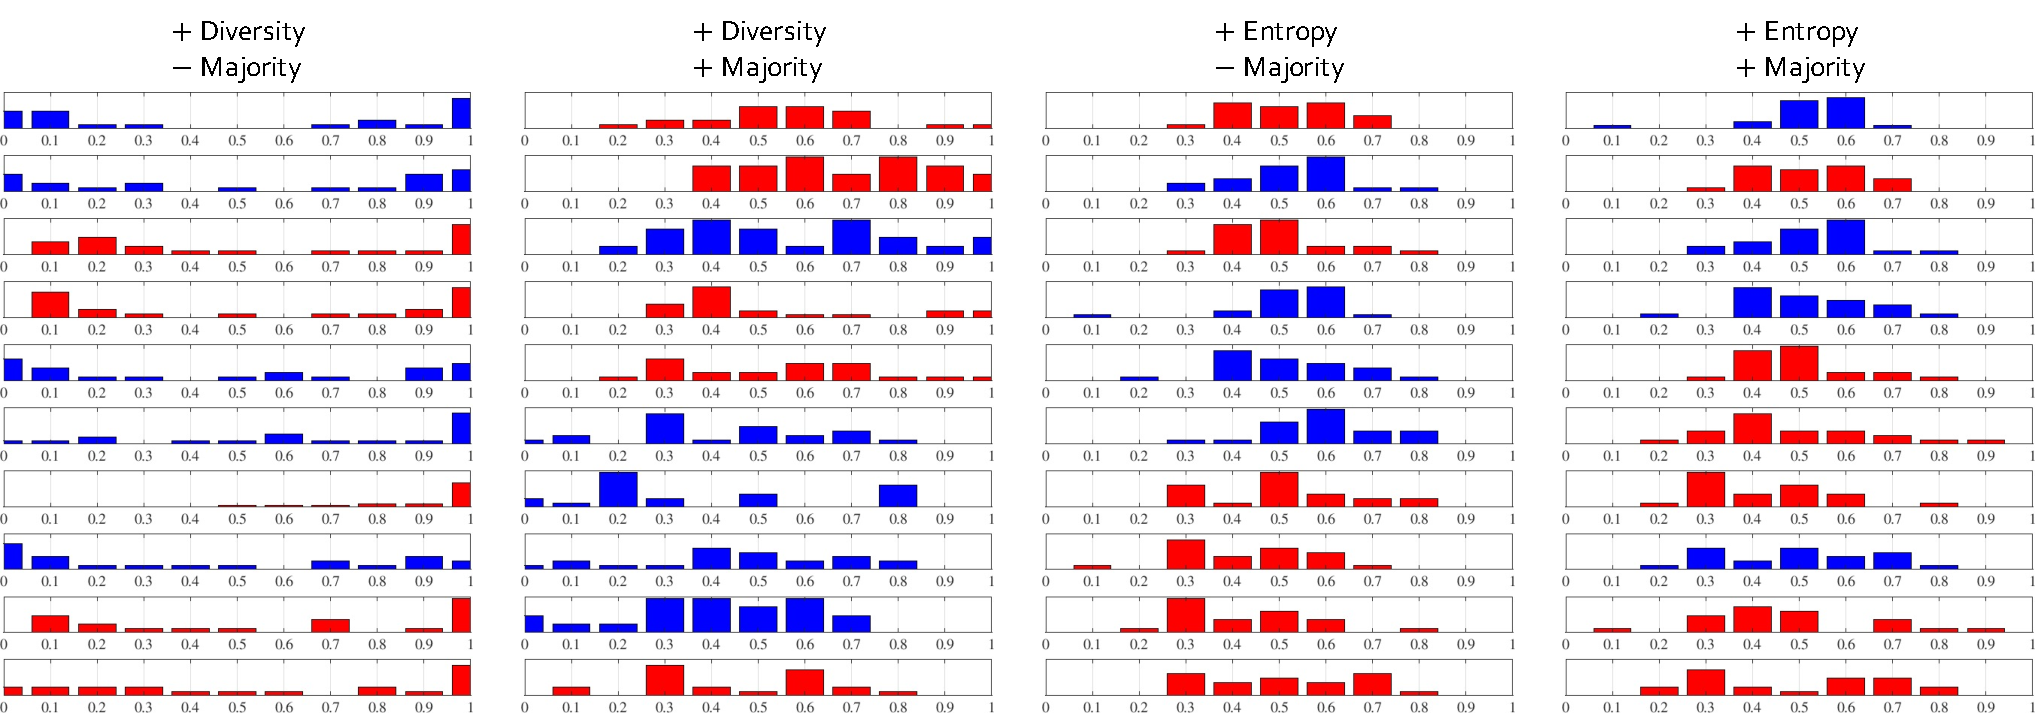
\includegraphics[width=1.0\columnwidth]{Figures/CH3/fig_predicted_distribution.pdf}
\end{center}
\caption[Prediction Distribution of Top Candidates]{
Distribution of predictions for the top ten candidates actively selected by the four ACFT methods at Step 3 in colonoscopy frame classification. Positive candidates are shown in red and negative candidates are shown in blue. This visualization confirms the assumption in \tableautorefname~\ref{ch3:tab:predict_pattern} that diversity+majority selection criteria prefers Pattern B whereas diversity suggests Pattern C; both entropy and entropy+majority favor Pattern A due to its higher degree of uncertainty. However, in this case at Step 3, with entropy+majority selection criteria, there are no more candidates with Pattern A; therefore, candidates with Pattern B are selected.
}
\label{ch3:fig:predicted_distribution}
\end{sidewaysfigure}

% \fillandplacepagenumber
% \end{landscape}
%%%%%%%%%%%%%%%%%%%%%%%%%%%%%%%%%%%%%%%%%%%%

\section{Discussion \& Conclusion}
\label{ch3:discussion_conclusion}



\subsection{What Are the Favored Prediction Patterns?}
\label{ch3:discussion_conclusion:favored_prediction_patterns}

\figurename~\ref{ch3:fig:places_examples} shows the active candidate selection process for multi-class classification. To facilitate comprehension, \tableautorefname~\ref{ch3:tab:predict_pattern} illustrates the process in the context of binary classification.
Assuming the prediction of patch $x^{j}_i$ by the current CNN is $P_i^{j}$, we call the histogram of $P_i^{j}, j \in [1, m]$ the prediction pattern of candidate $\mathcal{C}_i$. As shown in Row 1 of Table~\ref{ch3:tab:predict_pattern}, in binary classification, there are seven typical prediction patterns:
\begin{itemize}
\item Pattern A is mostly concentrated at 0.5, with a higher degree of uncertainty. Most active learning algorithms~\citep{settles2009active,guyon2011results} favor these types of candidates as they are effective for reducing uncertainty. 
\item Pattern B is flatter than Pattern A, as the patches' predictions are spread widely from 0 to 1 with a higher degree of inconsistency among the patches' predictions. Since all the patches belonging to a candidate are generated via data augmentation, they (at least the majority) are expected to make similar predictions. These types of candidates have the potential to significantly enhance the current CNN's performance.
\item Pattern C is clustered at the both ends, with a higher degree of diversity. These types of candidates are most likely associated with noisy labels at the patch level as illustrated in \figurename~\ref{ap1:fig:dataset_annotation}(c), and they are the least favorable for use in active selection because they may cause confusion when fine-tuning the CNN.
\item Patterns D and E are clustered at either end (\ie 0 or 1), with a higher degree of certainty. These types of candidates should not undergo annotation at this stage because it is likely the current CNN has correctly predicted them, and therefore these candidates would contribute very little towards fine-tuning the current CNN.
\item Patterns F and G have a higher degree of certainty for some of the patches' predictions but are associated with some outliers. These types of candidates are valuable because they are capable of smoothly improving the CNN's performance.  While such candidates might not make dramatic contributions, they do not significantly degrade the CNN's performance either.
\end{itemize}

\subsection{How Does Intra-diversity Differ from Inter-diversity?}
\label{ch3:discussion_conclusion:interdiversity_differ_from_interdiversity}

Since measuring diversity between selected samples and unlabeled samples is computationally intractable, especially for a large pool of data~\citep{sourati2016classification}, the existing diversity sampling cannot be applied directly to our real-world medical applications. To name a few, selection criteria $R$ in \citet{chakraborty2015active} involves all unlabeled samples (patches). There are 391,200 training patches for polyp detection, and computing their $R$ would demand 1.1 TB memory (391,00$^2\times$8). In addition, their algorithms for batch selection are based on the truncated power method~\citep{yuan2013truncated}, which is unable to find a solution even for our smallest application (colonoscopy frame classification with 42,000 training patches). \citet{holub2008entropy} cannot be directly used for our real-world applications either, as it has a complexity of $\mathcal{O}(L^3\times N^3)$ and requires to train $L\times N$ classifiers in each step, where $N$ indicates the number of unlabeled patches and $L$ indicates the number of classes. In addressing the computational complexity problem, we exploit the inherent consistency among the patches that are augmented from the same sample, making it feasible for our real-world applications. To contrast these two measures of diversity, the variance among samples refers to \textit{inter-diversity}, while the variance among patches augmented from the same sample refers to \textit{intra-diversity}. We recognize that intra-diversity would inevitably suffer from redundancy in selection, as it treats each sample separately and dismisses inter-diversity among samples. An obvious solution is to inject randomness into active selection criteria, as described in Sec.~\ref{ch3:approach_property:injecting_randomization_active_selection}. Nonetheless, a better solution is to combine inter- and intra-diversity together by computing inter-diversity locally on the smaller set of samples selected by intra-diversity. These solutions all aim at selecting sufficiently diverse samples with manageable computational complexity.


%%%%%%%%%%%%%%%%%%%%%%%%%%%%%%%%%%%%%%%%%%%%
\begin{figure}[t]
%\footnotesize
\begin{center}
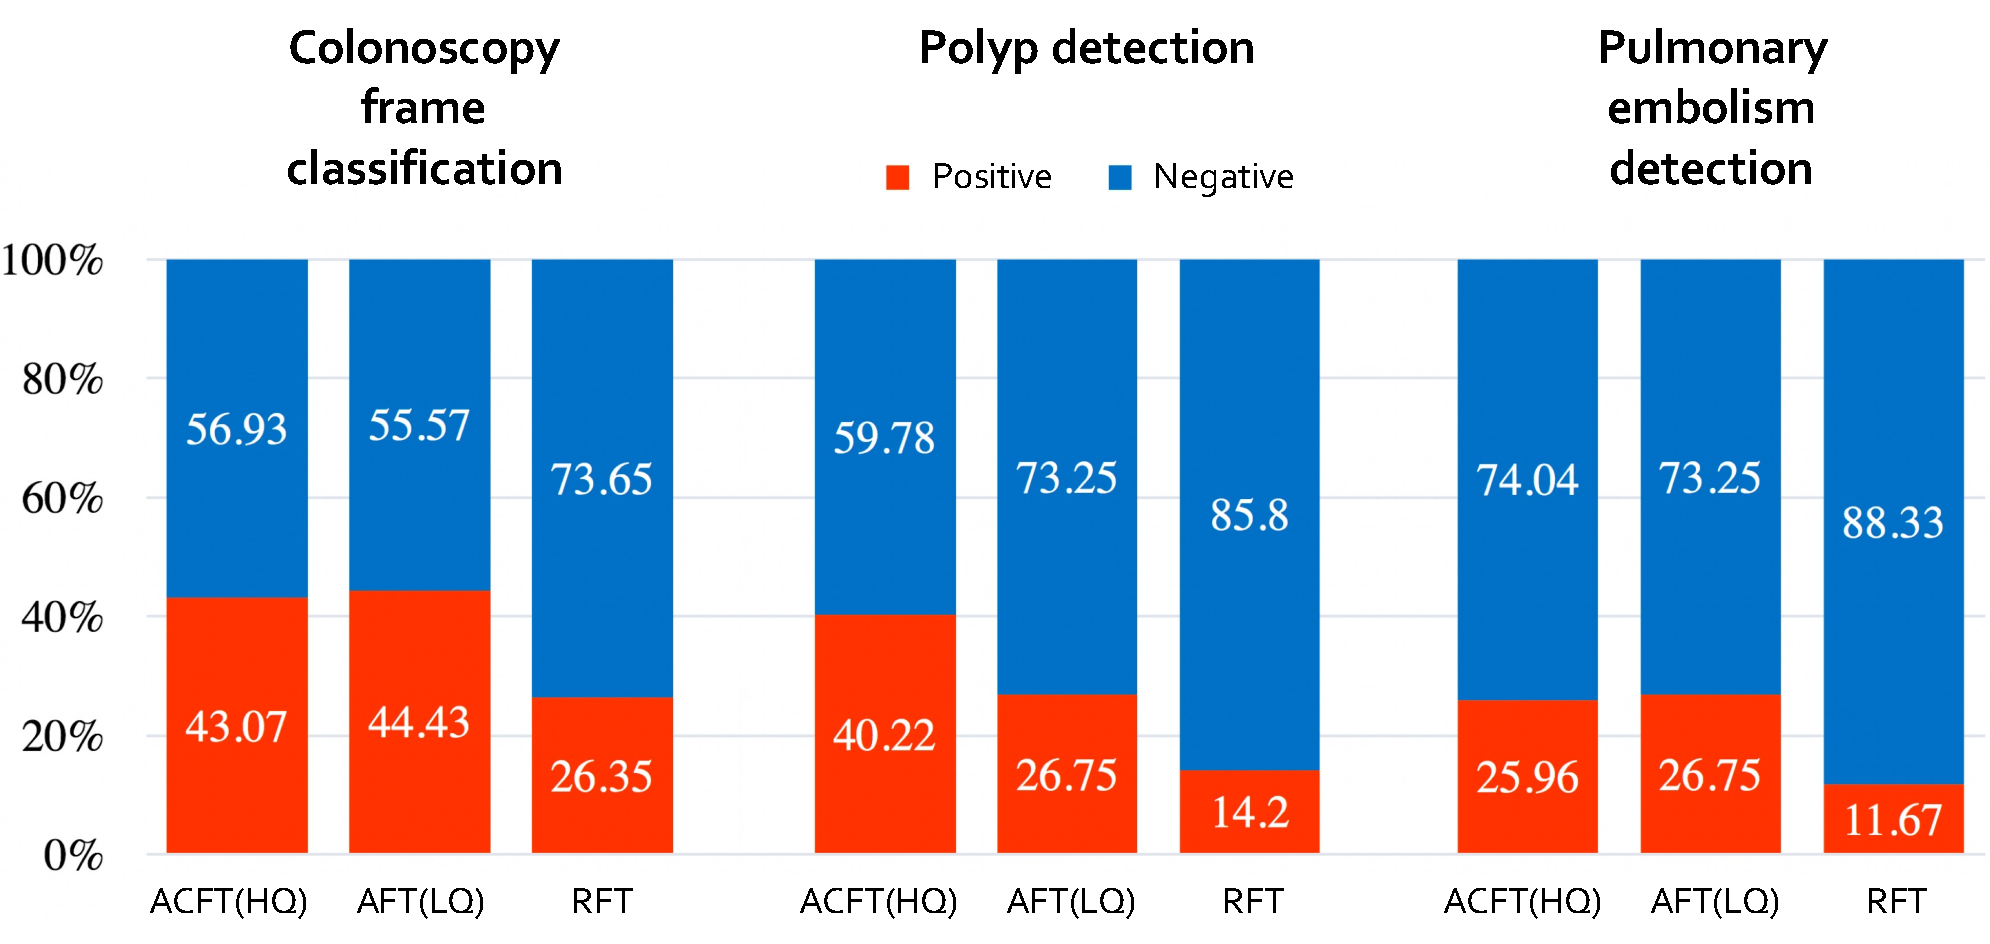
\includegraphics[width=0.9\linewidth]{Figures/CH3/fig_balance_ratio.pdf}
\end{center}
\caption[Positive/Negative Ratios of Selected Candidates]{
The positive/negative ratio in the candidates selected by ACFT, AFT and RFT. Please note that the ratio in RFT serves as an approximation for the ratio of the entire dataset.}
\label{ch3:fig:balance_ratio}
\end{figure}
%%%%%%%%%%%%%%%%%%%%%%%%%%%%%%%%%%%%%%%%%%%%

\subsection{Can Actively Selected Samples Be Automatically Balanced?}
\label{ch3:discussion_conclusion:samples_automatically_balanced}

Data is often imbalanced in real-world applications. The images of target classes of interest, \eg certain types of diseases, only appear in a small portion of the dataset. We encounter severe imbalances in our three applications. The ratio between positives and negatives is around 1:9 in the polyp and pulmonary embolism detection. Meanwhile, the ratio is approximately 3:7 in the colonoscopy frame classification. Learning from such imbalanced datasets leads to a common issue: majority bias~\citep{aggarwal2020active}, which is a prediction bias towards majority classes over minority classes. Training data should be balanced in terms of classes~\citep{japkowicz2002class,he2009learning,buda2018systematic}. Similar to most studies in active learning literature, our proposed selection criteria are not directly designed to tackle the issue of imbalance, but they have an implicit impact on balancing the data. For instance, when the current CNN has already learned more from positive samples, the next active learning selection would be more likely to prefer those negative samples, and vice-versa. On the contrary, random selection would consistently select new samples that follow roughly the same positive/negative ratio as the entire dataset. As shown in \figurename~\ref{ch3:fig:balance_ratio}, our ACFT$_{(HQ)}$ and AFT$_{(LQ)}$ are capable of automatically balancing the selected training data. After monitoring the active selection process, ACFT$_{(HQ)}$ and AFT$_{(LQ)}$ select twice as many positives compared to random selection. This does not suggest that the number of positives and negatives must be approximately identical in the selected samples. Negative samples naturally present more contextual variance than positive ones, as negatives can contain a vast array of possibilities not including the disease of interest. It is expected that the CNN should learn more from negatives to shape the decision boundary of positives. An ideal selection should cover a sufficient variety of negatives while striking an emphasis on the positives. We believe that this accounts for the quick achievement of superior performance in imbalanced data for our ACFT$_{(HQ)}$ and AFT$_{(LQ)}$.

%%%%%%%%%%%%%%%%%%%%%%%%%%%%%%%%%%%%%%%%%%%%
\begin{figure}[t]
%\footnotesize
\begin{center}
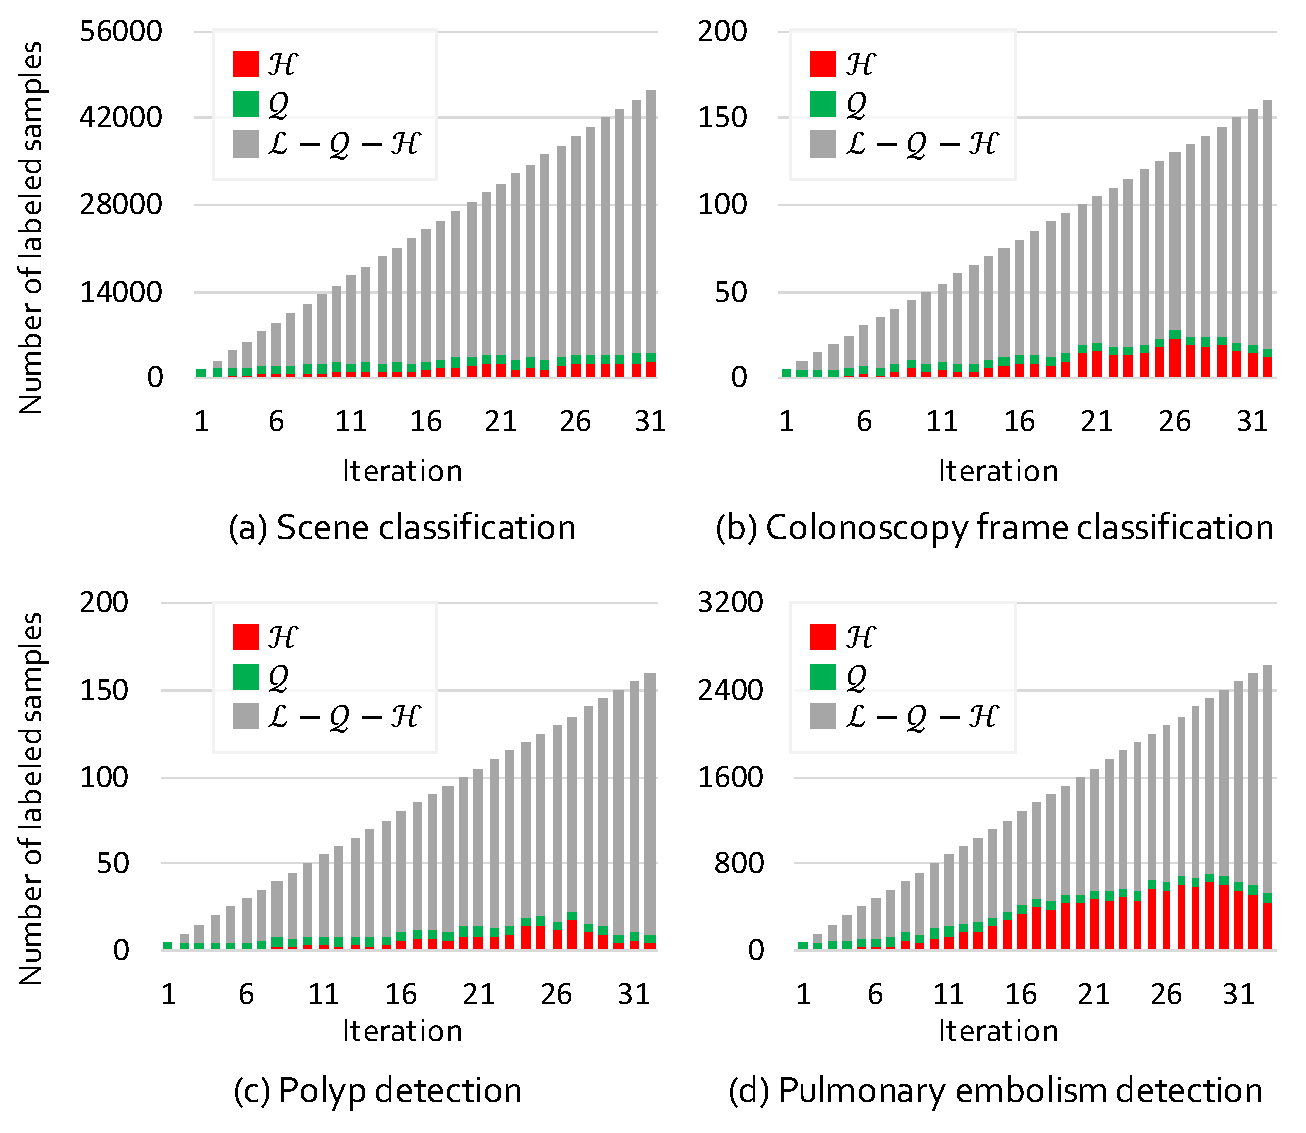
\includegraphics[width=0.75\linewidth]{Figures/CH3/fig_label_reuse.pdf}
\end{center}
\caption[Label Reusing in Active, Continual Fine-tuning]{
Labels are reused differently in four active learning strategies, as summarized in \tableautorefname~\ref{ch3:tab:terminology}. Specifically, the labels can be non-reused, partially reused, or 100\% reused. We plot the number of candidates along with each active learning step, including labeled candidates ($\mathcal{L}$), newly annotated candidates ($\mathcal{Q}$), and misclassified candidates ($\mathcal{H}$). As seen, by only continual fine-tuning on the hybrid data of $\mathcal{H}\bigcup\mathcal{Q}$, our ACFT significantly reduces training time through faster convergence than repeatedly fine-tuning on the entire labeled data of $\mathcal{L}\bigcup\mathcal{Q}$. Most importantly, as evidence by \tableautorefname~\ref{ch3:tab:main_results}, partially reusing labels can achieve compelling performance because it boosts performance by eliminating labeled easy candidates, focusing on hard ones, and preventing catastrophic forgetting.
}
\label{ch3:fig:label_reuse}
\end{figure}
%%%%%%%%%%%%%%%%%%%%%%%%%%%%%%%%%%%%%%%%%%%%

\subsection{How to Prevent Model Forgetting in Continual Learning?}
\label{ch3:discussion_conclusion:prevent_model_forgetting_continual_learning}

When a CNN learns from a stream of tasks continually, the learning of the new task can degrade the CNN's performance for earlier tasks~\citep{kirkpatrick2017overcoming,chen2018lifelong,parisi2019continual}. This phenomenon is called catastrophic forgetting, which was first recognized by~\citet{mccloskey1989catastrophic}. In our experiments, we have also observed similar behavior in active continual fine-tuning when the CNN encounters newly selected samples. This problem might not arise if the CNN is repeatedly trained on the entire labeled set at every active learning step. 
But fully reusing the labeled samples takes a lot of resources; further especially when the labeled set gets larger and larger, the impact of the newly selected samples on the model training becomes smaller and smaller (relative to the whole labeled set).
To make the training more efficient and maximize the contribution of new data, we attempted to fine-tune the CNN only on the newly selected samples, developing the learning strategy called ACFT$_{(Q)}$. However, as seen in~\tableautorefname~\ref{ch3:tab:main_results}, ACFT$_{(Q)}$ results in a substantially unstable performance because of the catastrophic forgetting. To track the forgotten samples, we have plotted a histogram of the misclassified candidates ($\mathcal{H}$) by the current CNN against labeled candidates ($\mathcal{L}$) and newly selected candidates ($\mathcal{Q}$) in~\figurename~\ref{ch3:fig:label_reuse}. We found that if the CNN is only fine-tuned on the newly selected samples at each step, it tends to forget the samples that have been learned from previous steps. This is because new data will likely override the weights that have been learned in the past, and thus overfitting the CNN on this data and degrading the model's generalizability. Therefore, we propose to combine the newly selected ($\mathcal{Q}$) and misclassified ($\mathcal{H}$) candidates together to continual fine-tune the current CNN, which not only spotlights the power of new data to achieve the comparable performance (see~\tableautorefname~\ref{ch3:tab:main_results}: ACFT$_{(HQ)}$ vs. AFT$_{(LQ)}$), but also eases the computational cost by eliminating re-training on easy samples, focusing on hard ones, and preventing catastrophic forgetting. 

\subsection{Is ACFT Generalizable to Other Models?}
\label{ch3:discussion_conclusion:generalizable_other_models}

We based our experiments on AlexNet and GoogLeNet. Alternatively, deeper architectures, such as VGG~\citep{simonyan2014very}, ResNet~\citep{he2016deep}, DenseNet~\citep{huang2017densely}, and FixEfficientNet~\citep{touvron2020fixing}, could have been used and they are known to show relatively higher performance for challenging computer vision tasks.
However, the purpose of this work is not to achieve the highest performance for different medical image tasks but to answer a critical question: {\em How can annotation costs be significantly reduced when applying CNNs to medical imaging?} For this purpose, we have experimented with our three applications, demonstrating consistent patterns between AlexNet and GoogLeNet as shown in \figurename~\ref{ch3:fig:selection_approaches_comparison_alexnet} and \figurename~\ref{ch3:fig:selection_approaches_comparison_googlenet}. As a result, given this generalizability, we can focus on comparing the prediction patterns and learning strategies rather than running experiments on different CNN architectures. Moreover, our active selection criteria only rely on data augmentation and model prediction, without being tied to specific types of predictors. This suggests that not only various CNN architectures, but also other predictive methods---spanning old fashions (\eg SVM, Random Forests, and AdaBoost) to recent trends such as CapsuleNet~\citep{sabour2017dynamic} and Transformer~\citep{dosovitskiy2020image}---can benefit from the progress in active learning.

\subsection{Can We Do Better on the Cold Start Problem?}
\label{ch3:discussion_conclusion:cold_start_problem}

It is crucial to intelligently select initial samples for an active learning procedure, especially for algorithms like our ACFT, which starts from a completely empty labeled dataset. Our results in \figurename~\ref{ch3:fig:selection_approaches_comparison_alexnet} and \figurename~\ref{ch3:fig:selection_approaches_comparison_googlenet} and several other studies~\citep{borisov2010active,zhou2017fine,yuan2020cold,gao2020consistency} reveal that uniformly, randomly selecting initial samples from the unlabeled set could outperform active selection at the beginning. This is one of the most challenging problems in active learning, known as the \textit{cold start} problem, which is ascribed to (1) data scarcity and (2) model instability at early stages. 
First, the data distribution in randomly selected samples better reflects the original distribution of the entire dataset than in actively selected samples. Maintaining a similar distribution between training and test data is beneficial when using scarce data. The most common practice is to admit the power of randomness at the beginning and randomly select initial samples from the unlabeled set~\citep{ren2020survey}. Our ACFT addresses the cold start problem by incorporating a random sampling probability with respect to the active selection criteria (as detailed in Sec.~\ref{ch3:approach_property:injecting_randomization_active_selection}). The devised ACFT (+randomness vs. -randomness in \figurename~\ref{ch3:fig:selection_approaches_comparison_alexnet} and \figurename~\ref{ch3:fig:selection_approaches_comparison_googlenet}) shows superior performance, even in early stages, with continued performance improving during the subsequent steps. 
Second, in the beginning, the CNN understandably fails to amply predict new samples, as it is trained with an inadequate number of samples. With horrible predictions, no matter how marvelous the selection criterion is, the selected samples would be unsatisfactory---as said ``garbage in garbage out''. To express meaningful CNN predictions, our ACFT suggests the use of pre-trained CNNs (as illustrated in Alg.~\ref{ch3:alg:ACFT}), not only initializing the CNN at the first step, but also providing fairly reasonable predictions for initial active selection. \figurename~\ref{ch3:fig:overall_result} presents encouraging results of active selection using pre-trained CNNs compared with random sampling from the unlabeled set (ACFT vs. RFT).
However, a CNN pre-trained on \textsc{ImageNet} may give poor predictions in the medical imaging domain, as it was trained from only {\em natural} images; it is associated with a large domain gap for medical images. As a result, the CNN predictions may be inconclusive or even opposite, yielding poor selection scores. Naturally, one may consider utilizing pre-trained models in the same domains to reduce this domain gap~\citep{zhou2021models,haghighi2020learning,feng2020parts2whole}. \citet{yuan2020cold} has demonstrated this idea in natural language processing by applying self-supervised language modeling to select initial samples. In the case of medical imaging, we naturally expect that self-supervised methods can also mitigate the pronounced domain gap between natural and medical imaging, offering a great starting point for selecting samples using domain-relevant image representation. More importantly, the learning objectives in self-supervised methods are applicable for discovering the most representative initial samples. 
For instance, our diversity criterion shares a similar spirit with the learning objective of BYOL~\citep{grill2020bootstrap} and of Parts2Whole~\citep{feng2020parts2whole}, as they all aim to pull together the patches augmented from the same sample.
Therefore, their objective functions could serve as an off-the-shelf measure for the power of a sample in elevating the pre-trained CNN's performance. The underlying hypothesis is that the worthiness of labeling a sample correlates with the learning objective of self-supervised pre-training. Specifically, a sample is potentially more worthy to train the CNN if it requires considerably more effort to perform the task of in-painting~\citep{pathak2016context}, restoration~\citep{zhou2021models}, contrastive learning~\citep{chen2020simple}, or colorization~\citep{zhang2016colorful}. We anticipate that self-supervised methods have great potential to accommodate the selection of initial samples by leveraging unlabeled data in the same domain, therefore, more effectively addressing the cold start problem in active learning. 

\subsection{Is Our Consistency Observation Useful for Other Purposes?}
\label{ch3:discussion_conclusion:consistency_observation_other_purposes}

Our key observation is that all patches augmented from the same sample share the same label, and thus are expected to have similar predictions by the CNN. This inherent invariance allows us to devise the diversity metric for estimating the worthiness of labeling the sample. From a broader view, the use of data consistency before and after a mixture of augmentation has played an important role in many other circumstances. In semi-supervised learning, the consistency loss serves as a bridge between labeled and unlabeled data. While the CNN is trained on labeled data, the consistency loss constrains predictions to be invariant to unlabeled data augmented in varying ways~\citep{yu2019uncertainty,cui2019semi,bortsova2019semi,fotedar2020extreme,gao2020consistency}. In self-supervised learning, the concept of consistency allows CNNs to learn transformation invariance features by either always restoring the original image from the transformed one~\citep{zhu2020rubik,zhou2021models} or explicitly pulling all patches augmented from the same image together in the feature space~\citep{feng2020parts2whole,chen2020simple,he2020momentum}. Albeit the great promises of consistency loss, automatic data augmentation inevitably generates ``noisy'' samples, jeopardizing the data consistency presumption. As an example, when an image contains objects A and B, random cropping may miss either one of the objects fully or partially, causing label inconsistency or representation inconsistency~\citep{purushwalkam2020demystifying,hinton2021represent}. Therefore, the choice of data augmentation is critical in employing the data consistency presumption. Other than data consistency, the prediction consistency of model ensembles can also calculate the diversity. For instance, \citet{gal2016dropout,gal2017deep,tsymbalov2018dropout} have proposed to estimate the prediction diversity presented in the CNN via Monte-Carlo dropout in the inference;~\citet{beluch2018power,yang2017suggestive,kuo2018cost,li2020transformation,venturini2020uncertainty} measure the prediction consistency by feeding images to multiple independent CNNs that have been trained for the same data and purpose. Unlike the data consistency in our work, their presumption is the model consistency, wherein the CNN predictions ought to be consistent if the same sample goes through the model ensembles; otherwise, this sample is considered worthy of labeling.


\subsection{Conclusion and Broader Impacts}
\label{ch3:discussion_conclusion:conclusion_broader_impacts}

We have developed a novel method for dramatically reducing annotation cost by integrating active learning and transfer learning. Compared with the state-of-the-art random selection method~\citep{tajbakhsh2016convolutional}, our method can reduce the annotation cost by at least half for three medical applications and by more than 33\% for natural image dataset \textsc{Places-3}. The superior performance of our method is attributable to eight distinct advantages, detailed in Sec.~\ref{ch3:approach_property:several_unique_properties}. We believe that labeling at the candidate level offers a sensible balance for our three applications, whereas labeling at the patient level would certainly enhance annotation cost reduction, but introduces more severe label noise. Labeling at the patch level compensates for additional label noise but would impose significant burdens on experts for annotation creation. More importantly, our method has the potential to positively impact computer-aided diagnosis (CAD) in medical imaging. The current regulations require that CAD systems be deployed in a ``closed'' environment, in which all CAD results are reviewed and errors, if any, must be corrected by radiologists. As a result, all false positives are dismissed and all false negatives are supplied, an instant on-line feedback process that makes it possible for CAD systems to be self-learning and self-improving after deployment given the continual fine-tuning capability of our method.

We presented this work in our CVPR paper~\citep{zhou2017fine} to integrate active learning and deep learning via continual fine-tuning. It has since been quickly adopted by the research community: reviewed by some of the most prestigious journals and conferences in the field~\citep{wang2018uncertainty,zhang2019attention,sourati2019intelligent,liu2019exploiting,bi2019active,zhang2019medical,budd2019survey}, served as competitive baseline~\citep{shi2019active,duan2019improved}, and enlightened to develop more advanced active learning approaches~\citep{zhou2019integrating,li2019reverse,zhang2019using}. Moreover, although the technique was derived from the medical context, it is a general active learning approach, which has been adopted in multiple alternative fields such as text classification~\citep{oftedal2019uncertainty}, vehicle type recognition~\citep{huang2019cost}, streaming recommendation system~\citep{guo2019streaming}, etc.



% \section*{Acknowledgements}

% I thank R. Todd Hurst for allowing us to test our ideas on the CIMT dataset.
\chapter{Utilizing Annotation from Advanced Models}
\label{ch4}

This chapter is based on the following publications:
\begin{itemize}
    \item Zhou, Z., Rahman Siddiquee M. M., Tajbakhsh, N., \& Liang, J. (2018). Unet++: A nested u-net architecture for medical image segmentation. In \textit{Deep learning in medical image analysis and multimodal learning for clinical decision support} (pp. 3-11). Springer, Cham.
    \item Zhou, Z., Rahman Siddiquee M. M., Tajbakhsh, N., \& Liang, J. (2019). Unet++: Redesigning skip connections to exploit multiscale features in image segmentation. \textit{IEEE transactions on medical imaging}, 39(6), 1856-1867.
\end{itemize}

% \section*{CRediT authorship contribution statement}

% I would like to thank all of the authors for their contributions and hard works. Md Mahfuzur Rahman Siddiquee: software, investigation, visualization. Nima Tajbakhsh: investigation, writing. Jianming Liang: conceptualization, methodology, formal analysis, investigation, resources, writing, supervision, project administration, funding acquisition. 

\newpage

\section{Background \& Motivation}
\label{ch4:background_motivation}



The encoder-decoder networks are widely used in modern semantic and instance segmentation models~\citep{zhou2017deep,shen2017deep,litjens2017survey,chartrand2017deep,falk2018u,tajbakhsh2020embracing}. Their success is largely attributed to their skip connections, which combine deep, semantic, coarse-grained feature maps from the decoder sub-network with shallow, low-level, fine-grained feature maps from the encoder sub-network, and have proven to be effective in recovering fine-grained details of the target objects~\citep{drozdzal2016importance,he2016deep,huang2017densely} even on complex background~\citep{hariharan2015hypercolumns,lin2017feature}. Skip connections have also played a key role in the success of instance-level segmentation models such as~\citet{he2017mask,hu2018learning} where the idea is to segment and distinguish each instance of desired objects. 

However, these encoder-decoder architectures for image segmentation come with two limitations. First, the optimal depth of an encoder-decoder network can vary from one application to another, depending on the task difficulty and the amount of labeled data available for training. A simple approach would be to train models of varying depths separately and then ensemble the resulting models during the inference time~\citep{dietterich2000ensemble,hoo2016deep,ciompi2015automatic}. However, this simple approach is inefficient from a deployment perspective, because these networks do not share a common encoder. Furthermore, being trained independently, these networks do not enjoy the benefits of multi-task learning~\citep{bengio2009learning,zhang2017survey}.
Second, the design of skip connections used in an encoder-decoder network is unnecessarily restrictive, demanding the fusion of the same-scale encoder and decoder feature maps. While striking as a natural design,  the same-scale feature maps from the decoder and encoder networks are semantically dissimilar and no solid theory guarantees that they are the best match for feature fusion. 



In this chapter, we present UNet++, a new general purpose image segmentation architecture that aims at overcoming the above limitations. As presented in~\figurename~\ref{ch4:fig:network_architecture}(g), UNet++ consists of U-Nets of varying depths whose decoders are densely connected at the same resolution via the redesigned skip connections. The architectural changes introduced in UNet++ enable the following advantages. First, UNet++ is not prone to the choice of network depth because it embeds U-Nets of varying depths in its architecture. All these U-Nets partially share an encoder, while their decoders are intertwined. By training UNet++ with deep supervision, all the constituent U-Nets are trained simultaneously while benefiting from a shared image representation. This design not only improves the overall segmentation performance, but also enables model pruning during the inference time. Second, UNet++ is not handicapped by unnecessarily restrictive skip connections where only the same-scale feature maps from the encoder and decoder can be fused. The redesigned skip connections introduced in  UNet++ present feature maps of varying scales at a decoder node, allowing the aggregation layer to decide how various feature maps carried along the skip connections should be fused with the decoder feature maps. The redesigned skip connections are realized in UNet++ by densely connecting the decoders of the constituents U-Nets at the same resolution.
We have extensively evaluated UNet++ across six segmentation datasets and multiple backbones of different depths. Our results demonstrate that UNet++ powered by redesigned skip connections and deep supervision enables a significantly higher level of performance for both semantic and instance segmentation. 
This significant improvement of UNet++ over the classical U-Net architecture is ascribed to the advantages offered by the redesigned skip connections and the extended decoders, which together enable gradual aggregation of the image features  across the network, both horizontally and vertically.

In summary, we make the following five contributions:
\begin{enumerate}
  \item We introduce a built-in ensemble of U-Nets of varying depths in UNet++, enabling improved segmentation performance for varying size objects---an improvement over the fixed-depth U-Net.
  \item We redesign skip connections in UNet++, enabling flexible feature fusion in decoders---an improvement over the restrictive skip connections in U-Net that require fusion of only same-scale feature maps.
  \item We devise a scheme to prune a trained UNet++, accelerating its inference speed while maintaining its performance.
  \item We discover that simultaneously training multi-depth U-Nets embedded within the UNet++ architecture stimulates collaborative learning among the constituent U-Nets, leading to much better performance than individually training isolated U-Nets of the same architecture.
  \item We demonstrate the extensibility of UNet++ to multiple backbone encoders and further its applicability to various medical imaging modalities including CT, MRI, and electron microscopy.
\end{enumerate}


%##############################################################################################
% \begin{landscape}
% \thispagestyle{empty}

\begin{sidewaysfigure}
\begin{center}
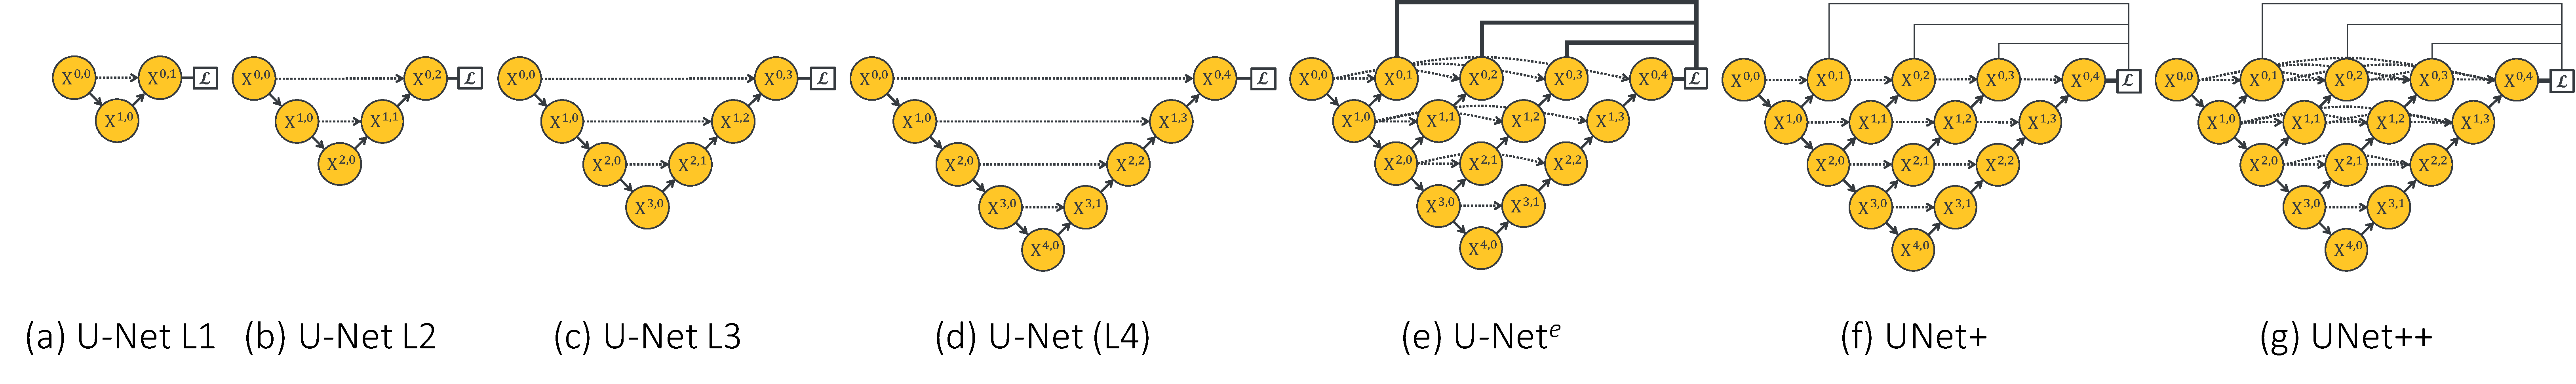
\includegraphics[width=1.0\columnwidth]{Figures/CH4/fig_architecture_evolution.pdf}
\end{center}
\caption[Evolution from U-Net to UNet++]{
Evolution from U-Net to UNet++. Each node in the graph represents a convolution block, downward arrows indicate down-sampling, upward arrows indicate up-sampling, and dot arrows indicate skip connections. (a--d) U-Nets of varying depths. (e) Ensemble architecture, U-Net$^e$, which combines U-Nets of varying depths into one unified architecture. All U-Nets (partially) share the same encoder, but have their own decoders.
(f) UNet+ is constructed from U-Net$^e$ by dropping the original skip connections and connecting every two adjacent nodes with a short skip connection, enabling the deeper decoders to send supervision signals to the shallower decoders. (g) UNet++ is constructed from U-Net$^e$ by connecting the decoders, resulting in densely connected skip connections, enabling dense feature propagation along skip connections and thus more flexible feature fusion at the decoder nodes.
As a result, each node in the UNet++ decoders, from a horizontal perspective, combines multiscale features from its all preceding nodes at the same resolution, and from a vertical perspective, integrates multiscale features across different resolutions from its preceding node, as formulated at Eq.~\ref{eq_unet}. This multiscale feature aggregation of UNet++ gradually synthesizes the segmentation, leading to increased accuracy and faster convergence, as evidenced by our empirical results in~\sectionname~\ref{ch4:experiments}.
Note that, explicit deep supervision is required (bold links) to train U-Net$^e$ but optional (pale links) for UNet+ and UNet++.}
\label{ch4:fig:network_architecture}
\end{sidewaysfigure}

% \fillandplacepagenumber
% \end{landscape}
%##############################################################################################


%##############################################################################################
\begin{table}[t]
\footnotesize
\begin{center}
\begin{threeparttable}
\caption[Ablation Study on U-Nets of Varying Depths]{
Ablation study on U-Nets of varying depths alongside with the new variants of U-Nets proposed in this work. U-Net L$d$ refers to a U-Net with a depth of $d$ (\figurename~\ref{ch4:fig:network_architecture}(a-d)). U-Net$^e$, UNet+, and UNet++ are the new variants of U-Net, which are depicted in \figurename~\ref{ch4:fig:network_architecture}(e-g). ``DS'' denotes deeply supervised training followed by average voting. Intersection over union (IoU) is used as the metric for comparison (mean$\pm$s.d. \%).}
\label{ch4:tab:architecture_analysis}
    \begin{tabular}{p{0.15\linewidth}P{0.04\linewidth}P{0.11\linewidth}P{0.16\linewidth}P{0.16\linewidth}P{0.2\linewidth}}
    \hline
    \textbf{Architecture} & \textbf{DS} & \textbf{Params} & \textbf{EM} & \textbf{Cell} & \textbf{Brain Tumor} \\
    \hline
    U-Net L$1$  & \xmark & 0.1M & 86.83{\tiny $\pm$0.43} & 88.58{\tiny $\pm$1.68} & 86.90{\tiny $\pm$2.25}  \\
    U-Net L$2$  & \xmark & 0.5M & 87.59{\tiny $\pm$0.34} & 89.39{\tiny $\pm$1.64} &  88.71{\tiny $\pm$1.45} \\
    U-Net L$3$   & \xmark & 1.9M & 88.16{\tiny $\pm$0.29} & 90.14{\tiny $\pm$1.57} & 89.62{\tiny $\pm$1.41}  \\
    U-Net (L$4$)  & \xmark & 7.8M & 88.30{\tiny $\pm$0.24} & 88.73{\tiny $\pm$1.64} & 89.21{\tiny $\pm$1.55} \\
    U-Net$^e$  & \cmark  & 8.7M & 88.33{\tiny $\pm$0.23} & 90.72{\tiny $\pm$1.51} &  90.19{\tiny $\pm$0.83} \\
    \hline
    UNet+  & \xmark & 8.7M & 88.39{\tiny $\pm$0.15} & 90.71{\tiny $\pm$1.25} & 90.70{\tiny $\pm$0.91}  \\
    UNet+  & \cmark & 8.7M & 88.89{\tiny $\pm$0.12} & 91.18{\tiny $\pm$1.13} & 91.15{\tiny $\pm$0.65} \\
    \hline
    UNet++  & \xmark & 9.0M & 88.92{\tiny $\pm$0.14} & 91.03{\tiny $\pm$1.34} & 90.86{\tiny $\pm$0.81}\\
    UNet++  & \cmark & 9.0M & \textbf{89.33{\tiny $\pm$0.10}} & \textbf{91.21{\tiny $\pm$0.98}} & {\bf 91.21{\tiny $\pm$0.68}} \\
    \hline
    \end{tabular}
\end{threeparttable}
\end{center}
\end{table}
%##############################################################################################


% \section{Redesigned Skip Connections for Multiscale Feature Aggregation}
\section{Approach \& Property}
\label{ch4:methods}

\figurename~\ref{ch4:fig:network_architecture} shows how UNet++ evolves from the original U-Net. In the following, we first trace this evolution, motivating the need for UNet++, and then explain its technical and implementation details.

\subsection{Evolving Architectural Designs}
\label{ch4:motiv}

We have done a comprehensive ablation study to investigate the performance of U-Nets of varying depths (\figurename~\ref{ch4:fig:network_architecture}(a-d)). For this purpose, we have used three relatively small datasets, namely \texttt{Cell}\footnote{I thank Michael G. Meyer for allowing us to test our ideas on the Cell-CT dataset.}, \texttt{EM}, and \texttt{Brain Tumor} (detailed in~Appendix~\ref{ap1}). \tableautorefname~\ref{ch4:tab:architecture_analysis} summarizes the results. For the cell and brain tumor segmentation, a shallower network (U-Net L$3$)\footnote{In this dissertation, the original notation U-Net/UNet+/UNet++ L$^{d}$ in \citet{zhou2018unet++,zhou2019unet++} has been replaced with U-Net/UNet+/UNet++ L${d}$ to avoid the confusion with footnote symbols.} outperforms the deep U-Net. For the EM dataset, on the other hand, the deeper U-Nets consistently outperform the shallower counterparts, but the  performance gain is only marginal. Our experimental results suggest two key findings: 1) deeper U-Nets are not necessarily always better, 2) the optimal depth of architecture depends on the difficulty and size of the dataset at hand. While these findings may encourage an automated neural architecture search, such an approach is hindered by the limited computational resources~\citep{liu2018progressive,zoph2018learning,liu2019auto,zhang2019customizable,li2019partial}. Alternatively, we propose an ensemble architecture, which combines  U-Nets of varying depths into one unified structure. We refer to this architecture as U-Net$^e$ (\figurename~\ref{ch4:fig:network_architecture}(e)). 
We train U-Net$^e$ by defining a separate loss function for each U-Net in the ensemble, \ie X$^{0,j},~j\in\{1,2,3,4\}$. Our deep supervision scheme differs from the commonly used deep supervision in deep image classification and image segmentation networks; in ~\citep{xie2015holistically,chen2016deep,dou20173d,lee2015deeply} the auxiliary loss functions are added to the nodes along the decoder network, \ie X$^{4-j,j},~j\in\{0,1,2,3,4\}$, whereas we apply them on X$^{0,j},~j\in\{1,2,3,4\}$. At the inference time, the output from each U-Net in the ensemble is averaged.


The ensemble architecture (U-Net$^e$) outlined above benefits from knowledge sharing, because all U-Nets within the ensemble partially share the same encoder even though they have their own  decoders. However, this architecture still suffers from two drawbacks. First, the decoders are disconnected---deeper U-Nets do not offer a supervision signal to the decoders of the shallower U-Nets in the ensemble. Second, the common design of skip connections used in the U-Net$^e$ is unnecessarily restrictive, requiring the network to combine the decoder feature maps with only the same-scale feature maps from the encoder. While striking as a natural design,  there is no guarantee that the same-scale feature maps are the best match for the feature fusion. 

To overcome the above limitations, we remove original skip connections from the U-Net$^e$ and connect every two adjacent nodes in the ensemble, resulting in a new architecture, which we refer to as UNet+ (\figurename~\ref{ch4:fig:network_architecture}(f)). Owing to the new connectivity scheme, UNet+ connects the disjoint decoders, enabling gradient back-propagation from the deeper decoders to the shallower counterparts. UNet+ further relaxes the unnecessarily restrictive behaviour of skip connections by presenting each node in the decoders with the aggregation of all feature maps computed in the shallower stream. While using aggregated feature maps at a decoder node is far less restrictive than having only the same-scale feature map from the encoder,  there is still room for improvement. We further propose to use dense connectivity in UNet+,  resulting in our final architecture proposal, which we refer to as UNet++ (\figurename~\ref{ch4:fig:network_architecture}(g)). With dense connectivity, each node in a decoder is presented with not only the final aggregated feature maps but also with the intermediate aggregated feature maps and the original same-scale feature maps from the encoder. As such, the aggregation layer in the decoder node may learn to use only the same-scale encoder feature maps or use all collected feature maps available at the gate.
Unlike U-Net$^e$, deep supervision is not required for UNet+ and UNet++, however, as we will describe later, deep supervision enables model pruning during the inference time, leading to a significant speedup with only modest drop in  performance.

\subsection{Redesigning Skip Connections}
\label{ch4:model}

Let $x^{i,j}$ denote the output of node X$^{i,j}$ where $i$ indexes the down-sampling layer along the encoder and $j$ indexes the convolution layer of the dense block along the skip connection. The stack of feature maps represented by $x^{i,j}$ is computed as
\begin{equation}
\label{eq_unet}
    x^{i,j}=\begin{cases}
      \mathcal{H}\left(\mathcal{D}(x^{i-1,j})\right),  & j=0  \\
      \mathcal{H}\left(\left[\left[x^{i,k}\right]_{k=0}^{j-1}, \mathcal{U}(x^{i+1,j-1}) \right]\right), & j>0  \\
    \end{cases}
\end{equation}
where function $\mathcal{H}(\cdot)$ is a convolution operation followed by an activation function, $\mathcal{D}(\cdot)$ and $\mathcal{U}(\cdot)$ denote a down-sampling layer and an up-sampling layer respectively, and $[$ $]$ denotes the concatenation layer. Basically, as shown in~\figurename~\ref{ch4:fig:network_architecture}(g), nodes at level $j=0$  receive only one input from the previous layer of the encoder; nodes at level $j=1$ receive two inputs, both from the encoder sub-network but at two consecutive levels; and nodes at level $j>1$ receive $j+1$ inputs, of which $j$ inputs are the outputs of the previous $j$ nodes in the same skip connection and the $j+1^{th}$ input is the up-sampled output from the lower skip connection. The reason that all prior feature maps accumulate and arrive at the current node is because we make use of a dense convolution block along each skip connection.

%##############################################################################################
\begin{figure}[t]
\begin{center}
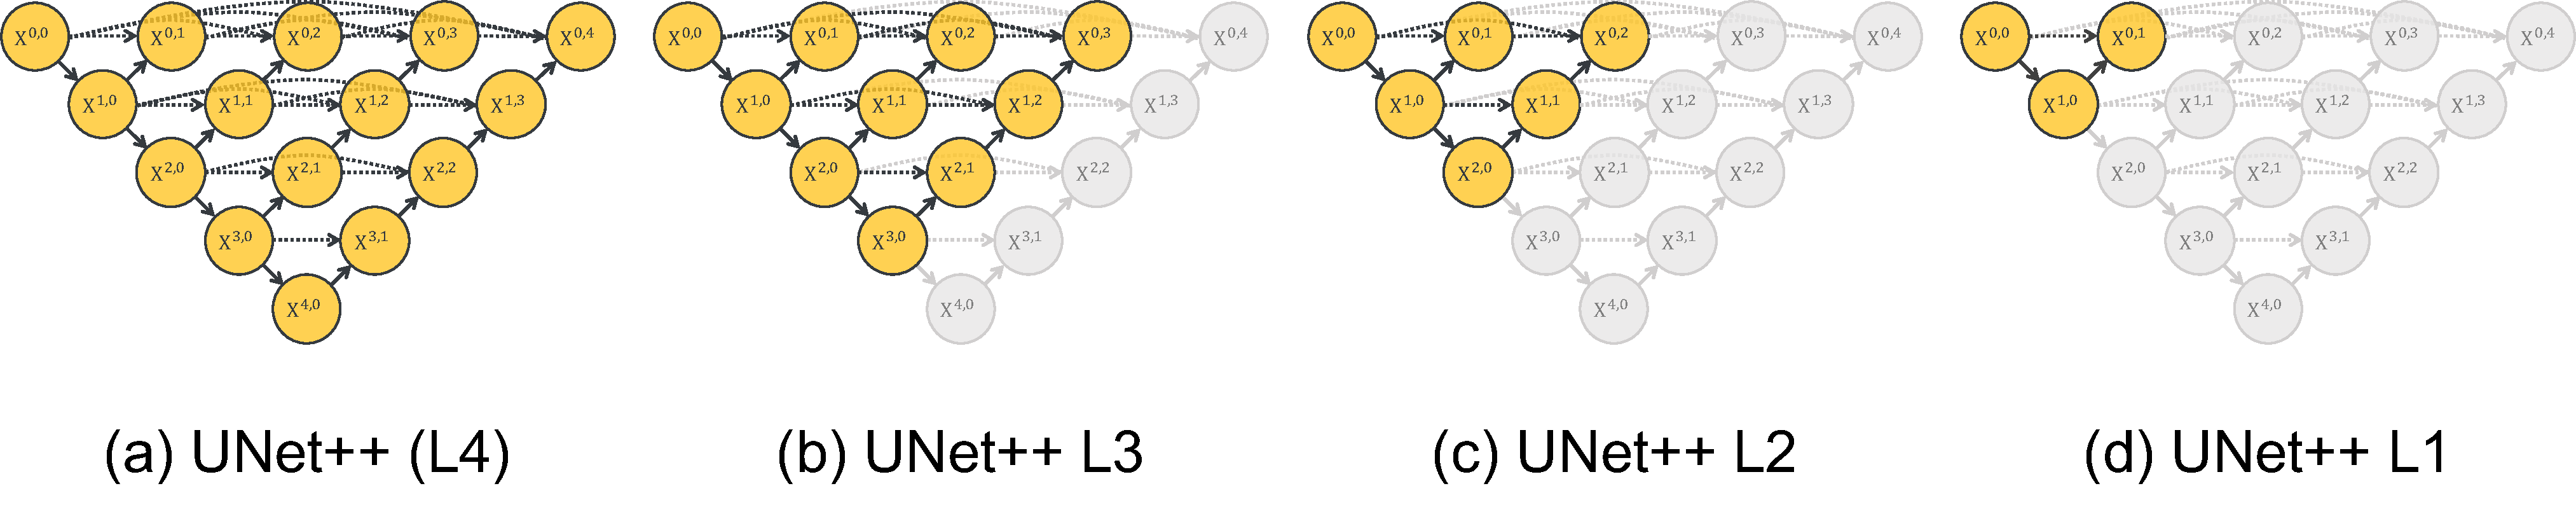
\includegraphics[width=1.0\linewidth]{Figures/CH4/fig_pruned_structure.pdf}
\end{center}
\caption[Deep Supervision Enables Model Pruning]{
Training UNet++ with deep supervision makes segmentation results available at multiple nodes X$^{0,j}$, enabling architecture pruning at inference time. Taking the segmentation result from X$^{0,4}$ leads to no pruning, UNet++ (L$4$),  whereas taking the segmentation result from X$^{0,1}$ results in a maximally pruned architecture, UNet++ L$1$. Note that nodes removed during pruning are colored in gray.}
\label{ch4:fig:prune_structure}
\end{figure}
%##############################################################################################


\subsection{Introducing Deep Supervision}
We introduce deep supervision in UNet++. For this purpose, we append a 1$\times$1 convolution with $\mathcal{C}$ kernels followed by a \textit{Sigmoid} activation function to the outputs from nodes  X$^{0,1}$, X$^{0,2}$, X$^{0,3}$, and X$^{0,4}$ where $\mathcal{C}$ is the number of classes observed in the given dataset. We then define a hybrid segmentation loss consisting of pixel-wise cross-entropy loss and soft dice-coefficient loss for each semantic scale. The hybrid loss may take advantages of what both loss functions have to offer: smooth gradient and handling of class imbalance~\citep{milletari2016v,sudre2017generalised}. Mathematically, the hybrid loss is defined as: 

\begin{equation}
\label{eq:object_function}
\mathcal{L}(Y,P) = -\frac{1}{N}\sum_{c=1}^{\mathcal{C}}\sum_{n=1}^{N}{\left(y_{n,c}\log{p_{n,c}}+\frac{2y_{n,c}p_{n,c}}{y^2_{n,c}+p^2_{n,c}}\right)}
\end{equation}
\noindent where $y_{n,c}\in Y$ and $p_{n,c}\in P$ denote the target labels and predicted probabilities for class $c$ and $n^{th}$ pixel in the batch, $N$ indicates the number of pixels within one batch. The overall loss function for UNet++ is then defined as the weighted summation of the hybrid loss from each individual decoders: $\mathcal{L}=\sum_{i=1}^{d}{\eta_i\cdot \mathcal{L}(Y,P^i)}$, where $d$ indexes the decoder. In the experiments, we give same balanced weights $\eta_i$ to each loss, \ie $\eta_i\equiv 1$, and do not process the ground truth for different outputs supervision like Gaussian blur.

Deep supervision enables model pruning. Owing to deep supervision, UNet++ can be deployed in two operation modes: 1) ensemble mode where the segmentation results from all segmentation branches are collected and then averaged, and 2) pruned mode where the segmentation output is selected from only one of the segmentation branches, the choice of which determines the extent of model pruning and speed gain.  \figurename~\ref{ch4:fig:prune_structure} shows how the choice of the segmentation branch results in pruned architectures of varying complexity. Specifically, taking the segmentation result from X$^{0,4}$ leads to no pruning whereas taking the segmentation result from X$^{0,1}$ leads to maximal pruning of the network.


\subsection{Two Unique Properties}
\label{ch4:approach_property:several_unique_properties}

\begin{enumerate}

    \item \textit{UNet++ enables multi-scale feature aggregation.} The original U-Net carried residual connections between the encoder and decoder, while our UNet++ suggests dense connections in between, reducing semantic gaps and encouraging feature reuse. This idea can be adapted to the original U-Net, the U-Nets with various backbones as feature extractors, and other segmentation frameworks such as Mask RCNN.
    
    \item \textit{UNet++ introduces deep supervision.} Multiple branches in the UNet++ are collaboratively trained with deep supervision at the full resolution. Deep supervision can stabilize the model training and explore the most effective features for varying sizes of lesions. Moreover, deep supervision makes segmentation outputs available at multiple branches, enabling architecture pruning at inference time.
    
    
\end{enumerate}

%##############################################################################################
\begin{table}[t]
\footnotesize
\centering
\caption[Parameter Settings of U-Net, Wide U-Net, UNet+, and UNet++]{
Details of the architectures used in our study. Wider version of U-Net and V-Net are designed to have comparable number of parameters to UNet++ and VNet++.}
\label{ch4:tab:wide_unet} %
\begin{tabular}{P{0.23\linewidth}P{0.12\linewidth}P{0.09\linewidth}P{0.09\linewidth}P{0.09\linewidth}P{0.09\linewidth}P{0.09\linewidth}}
    \hline
    \multirow{2}*{\textbf{Architecture}} & \multirow{2}*{\textbf{Params}} & \textbf{X$^{0,0}$} & \textbf{X$^{1,0}$} & \textbf{X$^{2,0}$} & \textbf{X$^{3,0}$} & \textbf{X$^{4,0}$} \\
     &  & \textbf{X$^{0,4}$} & \textbf{X$^{1,3}$} & \textbf{X$^{2,2}$} & \textbf{X$^{3,1}$} & \textbf{X$^{4,0}$} \\
    \hline
    U-Net & 7.8M &32 & 64 & 128 & 256 & 512 \\
    wide U-Net & 9.1M & 35 & 70 & 140 & 280 & 560 \\
    V-Net & 22.6M & 32 & 64 & 128 & 256 & 512 \\
    wide V-Net & 27.0M & 35 & 70 & 140 & 280 & 560 \\
    \hline
    \textbf{Architecture} & \textbf{Params} & \textbf{X$^{0,0-4}$} & \textbf{X$^{1,0-3}$} & \textbf{X$^{2,0-2}$} & \textbf{X$^{3,0-1}$} & \textbf{X$^{4,0}$} \\
    \hline
    UNet+ & 8.7M &32 & 64 & 128 & 256 & 512 \\
    UNet++ & 9.0M &32 & 64 & 128 & 256 & 512 \\
    VNet+ & 25.3M & 32 & 64 & 128 & 256 & 512 \\
    VNet++ & 26.2M & 32 & 64 & 128 & 256 & 512 \\
    \hline
\end{tabular}
\end{table}
%##############################################################################################


\section{Experiment \& Result}
\label{ch4:experiments}



\subsection{Benchmarking UNet++}
\label{ch4:implementation}

For comparison, we use the original U-Net~\citep{ronneberger2015u} and a customized wide U-Net architecture for 2D segmentation tasks, and V-Net~\citep{milletari2016v} and a customized wide V-Net architecture for 3D segmentation tasks. We choose U-Net (or V-Net for 3D) because it is a common performance baseline for image segmentation. We have also designed a wide U-Net (or wide V-Net for 3D) with a similar number of parameters to our suggested architecture. This is to ensure that the performance gain yielded by our architecture is \textit{not} simply due to the increased number of parameters. \tableautorefname~\ref{ch4:tab:wide_unet} details the U-Net and wide U-Net architectures. We have further compared the performance of UNet++ against UNet+, which is our intermediate architecture proposal. The numbers of kernels in the intermediate nodes have been given in~\tableautorefname~\ref{ch4:tab:wide_unet}. 


%%%%%%%%%%%%%%%%%%%%%%%%%%%%%%%%%%%%%%%%%%%%
% \begin{landscape}
% \thispagestyle{empty}

\begin{sidewaystable}
\begin{threeparttable}[t]
\scriptsize
\begin{center}
    \caption[UNet++ Outperforms U-Net in Semantic Segmentation]{
    Semantic segmentation results measured by IoU (mean$\pm$s.d.) for U-Net, wide U-Net, UNet+ (our intermediate proposal), and  UNet++ (our final proposal). Both UNet+ and UNet++ are evaluated with and without deep supervision (DS). We have performed independent two sample $t$-test between U-Net~\cite{falk2018u} vs. others for 20 independent trials and highlighted boxes in red when the differences are statistically significant ($p<0.05$).}
    \label{ch4:tab:main_results}
    \begin{tabular}{P{0.09\linewidth}P{0.01\linewidth}P{0.05\linewidth}|P{0.07\linewidth}P{0.07\linewidth}P{0.07\linewidth}P{0.07\linewidth}P{0.07\linewidth}|P{0.09\linewidth}P{0.01\linewidth}P{0.05\linewidth}|P{0.11\linewidth}}
    \hline
    \multirow{2}*{\textbf{Architecture}} & \multirow{2}*{\textbf{DS}} & \multirow{2}*{\textbf{Params}} & \multicolumn{5}{c|}{\textbf{2D Application}} & \multirow{2}*{\textbf{Architecture}} & \multirow{2}*{\textbf{DS}} & \multirow{2}*{\textbf{Params}} & \textbf{3D Application} \\
    \cline{4-8}\cline{12-12}
     & & &  \textbf{EM} & \textbf{Cell} & \textbf{Nuclei} & \textbf{BraTS} & \textbf{Liver} & & & & \textbf{Lung Nodule} \\
    \hline
    U-Net & \xmark & 7.8M & 88.30{\tiny $\pm$0.24} & 88.73{\tiny $\pm$1.64} & 90.57{\tiny $\pm$1.26} & 89.21{\tiny $\pm$1.55} & 79.90{\tiny $\pm$1.38} & V-Net & \xmark & 22.6M & 71.17{\tiny $\pm$4.53} \\
    wide U-Net & \xmark & 9.1M & 88.37{\tiny $\pm$0.13} & 88.91{\tiny $\pm$1.43} & 90.47{\tiny $\pm$1.15} & 89.35{\tiny $\pm$1.49}  & 80.25{\tiny $\pm$1.31} & wide V-Net & \xmark & 27.0M & 73.12{\tiny $\pm$3.99} \\
    UNet+ & \xmark & 8.7M & 88.39{\tiny $\pm$0.15} & \cellcolor{maroon!15}90.71{\tiny $\pm$1.25} & \cellcolor{maroon!15}91.73{\tiny $\pm$1.09} & \cellcolor{maroon!15}90.70{\tiny $\pm$0.91} & 79.62{\tiny $\pm$1.20} & VNet+ & \xmark & 25.3M & \cellcolor{maroon!15}75.93{\tiny $\pm$2.93} \\
    UNet+ & \cmark & 8.7M & \cellcolor{maroon!15}88.89{\tiny $\pm$0.12} & \cellcolor{maroon!15}91.18{\tiny $\pm$1.13} & \cellcolor{maroon!15}92.04{\tiny $\pm$0.89} & \cellcolor{maroon!15}91.15{\tiny $\pm$0.65} & \cellcolor{maroon!15}\textbf{82.83{\tiny $\pm$0.92}} & VNet+ & \cmark & 25.3M & \cellcolor{maroon!15}76.72{\tiny $\pm$2.48} \\
    UNet++ & \xmark & 9.0M & \cellcolor{maroon!15}88.92{\tiny $\pm$0.14} & \cellcolor{maroon!15}91.03{\tiny $\pm$1.34} &  \cellcolor{maroon!15}\textbf{92.44{\tiny $\pm$1.20}} & \cellcolor{maroon!15}90.86{\tiny $\pm$0.81}&	\cellcolor{maroon!15}82.51{\tiny $\pm$1.29} & VNet++ & \xmark & 26.2M & \cellcolor{maroon!15}76.24{\tiny $\pm$3.11}\\
    UNet++ & \cmark & 9.0M & \cellcolor{maroon!15}\textbf{89.33{\tiny $\pm$0.10}} & \cellcolor{maroon!15}\textbf{91.21{\tiny $\pm$0.98}}  & \cellcolor{maroon!15}92.37{\tiny $\pm$0.98} & \cellcolor{maroon!15}\textbf{91.21{\tiny $\pm$0.68}}	& \cellcolor{maroon!15}82.60{\tiny $\pm$1.11} & VNet++ & \cmark & 26.2M & \cellcolor{maroon!15}\textbf{77.05{\tiny $\pm$2.42}}\\
    \hline
    \end{tabular}
    \begin{tablenotes}
        \scriptsize
        \item[1] The winner in BraTS-2013 holds a ``complete'' Dice of 92\%  vs. 90.83$\%\pm$2.46\% (our UNet++ with deep supervision).
    \end{tablenotes}
\end{center}
\end{threeparttable}
\end{sidewaystable}
% \fillandplacepagenumber
% \end{landscape}
%%%%%%%%%%%%%%%%%%%%%%%%%%%%%%%%%%%%%%%%%%%%


%##############################################################################################
% \begin{landscape}
% \thispagestyle{empty}

\begin{sidewaysfigure}
\begin{center}
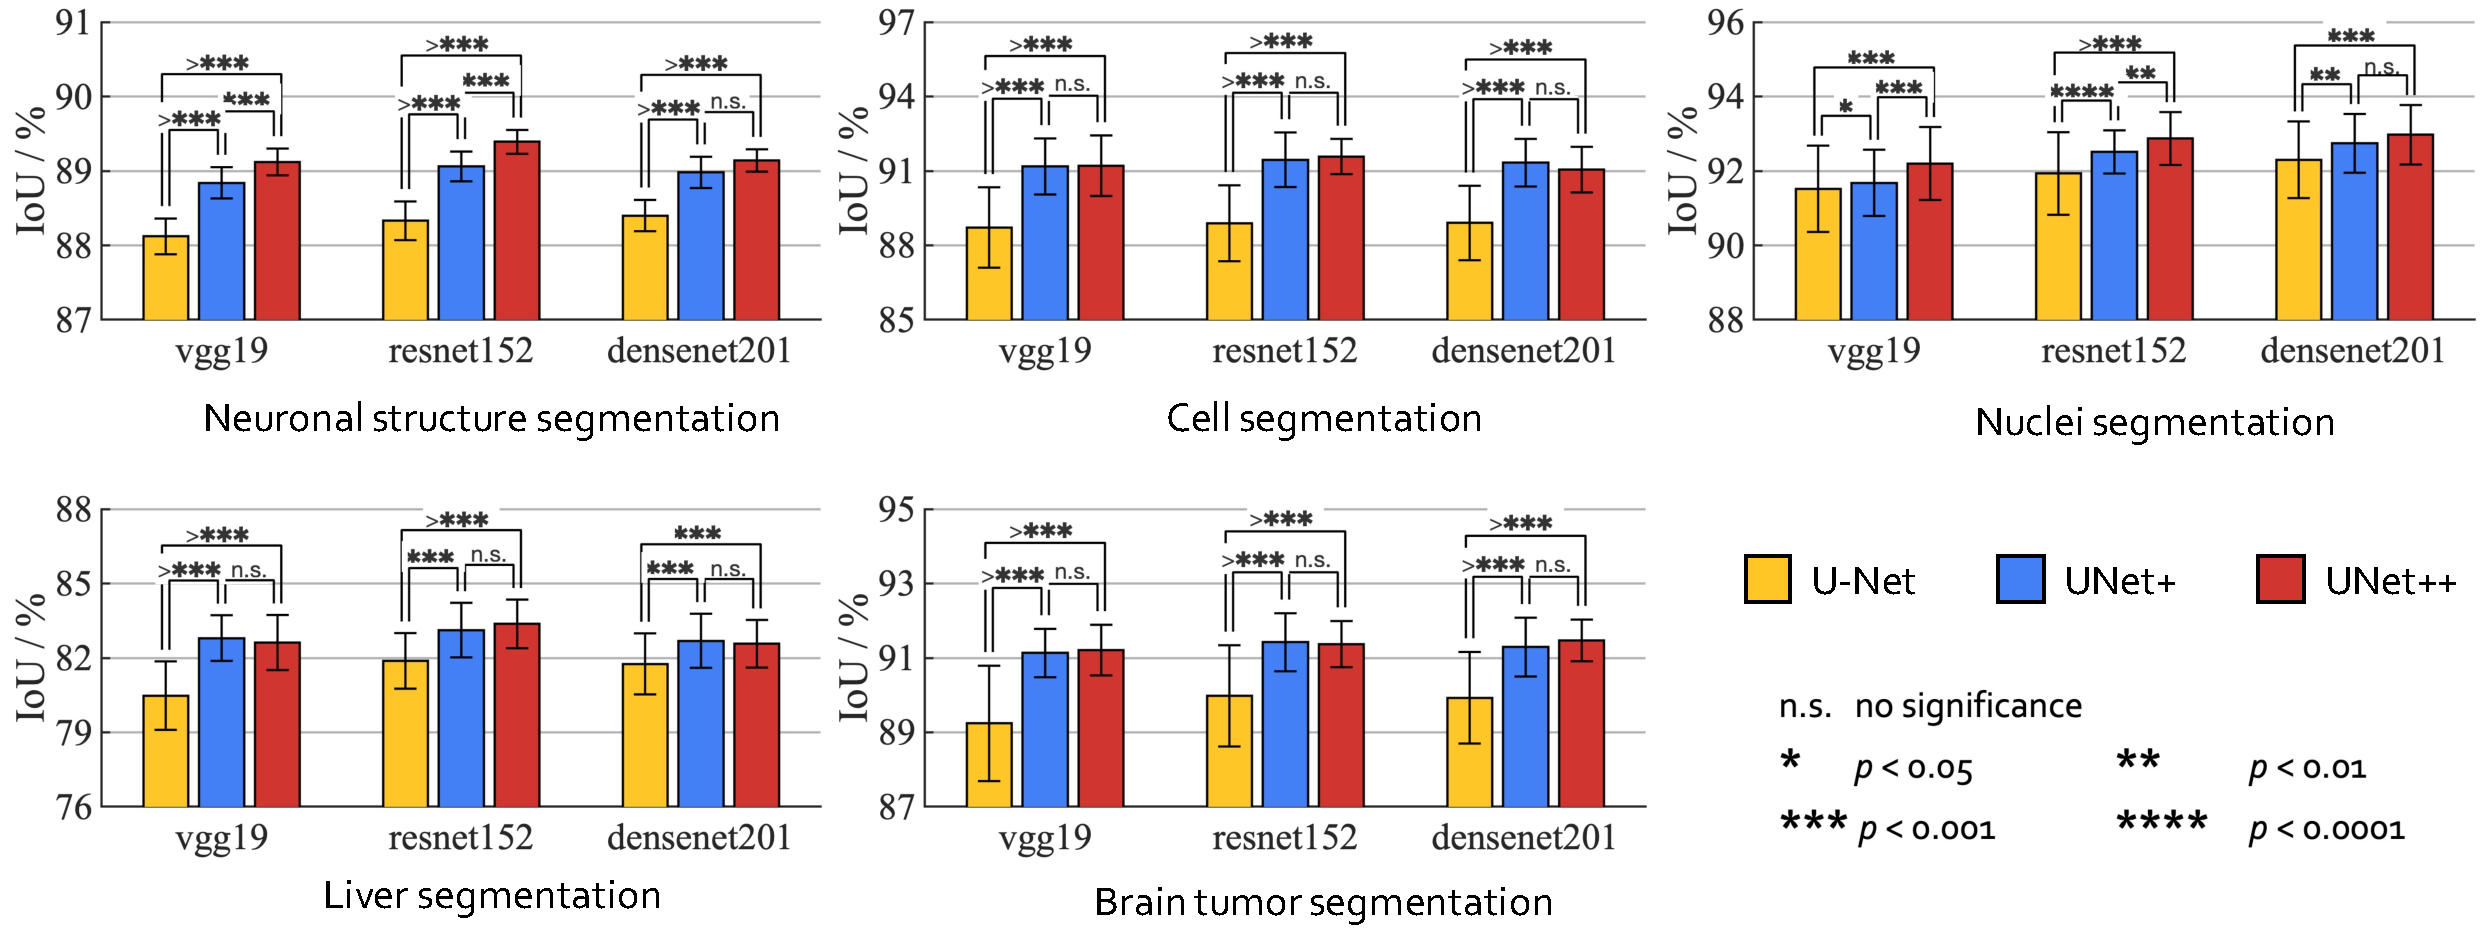
\includegraphics[width=1.0\columnwidth]{Figures/CH4/fig_various_backbones.pdf}
\end{center}
\caption[Comparison of U-Net, UNet+, and UNet++ with Varying Backbones]{
Comparison between U-Net, UNet+, and UNet++ when applied to the state-of-the-art backbones for the tasks of neuronal structure, cell, nuclei, brain tumor, and liver segmentation.
UNet++, trained with deep supervision, consistently outperforms U-Net across all backbone architectures and applications under study. By densely connecting the intermediate layers, UNet++ also yields higher segmentation performance than UNet+ in most experimental configurations.
The error bars represent the 95\% confidence interval and the number of $\ast$ on the bridge indicates the level of significance measured by $p$-value (``n.s.'' stands for ``not statistically significant'').}
\label{ch4:fig:various_backbones}
\end{sidewaysfigure}

% \fillandplacepagenumber
% \end{landscape}
%##############################################################################################


\subsection{UNet++ Outperforms U-Net in Semantic Segmentation}
\label{ch4:semantic_results}

\tableautorefname~\ref{ch4:tab:main_results} compares U-Net, wide U-Net, UNet+, and UNet++ in terms of the number parameters and segmentation results measured by IoU (mean$\pm$s.d) for the six segmentation tasks under study. As seen, wide U-Net consistently outperforms U-Net. This improvement is attributed to the larger number of parameters in wide U-Net. UNet++ without deep supervision achieves a significant IoU gain over both U-Net and wide U-Net for all the six tasks of neuronal structure ($\uparrow$0.62$\pm$0.10, $\uparrow$0.55$\pm$0.01), cell ($\uparrow$2.30$\pm$0.30, $\uparrow$2.12$\pm$0.09), nuclei ($\uparrow$1.87$\pm$0.06, $\uparrow$1.71$\pm$0.06), brain tumor ($\uparrow$2.00$\pm$0.87, $\uparrow$1.86$\pm$0.81), liver\footnote{I acknowledge Md Mahfuzur Rahman Siddiquee, with whom I co-authored~\citet{zhou2018unet++,zhou2019unet++}, for conducting the experiments and providing the results for liver segmentation.} ($\uparrow$2.62$\pm$0.09, $\uparrow$2.26$\pm$0.02), and lung nodule ($\uparrow$5.06$\pm$1.42, $\uparrow$3.12$\pm$0.88) segmentation. Using deep supervision and average voting further improves UNet++, increasing the IoU by up to 0.8 points. Specifically, neuronal structure and lung nodule segmentation benefit the most from deep supervision because they appear at varying scales in EM and CT slices.
Deep supervision, however, is only marginally effective for other datasets at best.  \figurename~\ref{ch4:fig:predict_visualization} depicts a qualitative comparison between the results of U-Net, wide U-Net, and UNet++. 

We have further investigated the extensibility of UNet++ for semantic segmentation by applying redesigned skip connections to an array of modern CNN architectures: vgg-19~\citep{simonyan2014very}, resnet-152~\citep{he2016deep}, and densenet-201~\citep{huang2017densely}. Specifically, we have turned each architecture above into a U-Net model by adding a decoder sub-network, and then replaced the plain skip connections of U-Net with the redesigned connections of UNet++. For comparison, we have also trained U-Net and  UNet+ with the aforementioned backbone architectures. 
For a comprehensive comparison, we have used \texttt{EM}, \texttt{Cell}, \texttt{Nuclei}, \texttt{Brain Tumor} and \texttt{Liver} segmentation datasets.
As seen in \figurename~\ref{ch4:fig:various_backbones}, UNet++ consistently outperforms U-Net and UNet+ across all backbone architectures and applications under study.
Through 20 trials, we further present a statistical analysis based on the independent two-sample $t$-test on each pair among U-Net, UNet+, and UNet++.
Our results suggest that UNet++ is an effective, backbone-agnostic extension to U-Net. 


%##############################################################################################
\begin{figure}[t]
\begin{center}
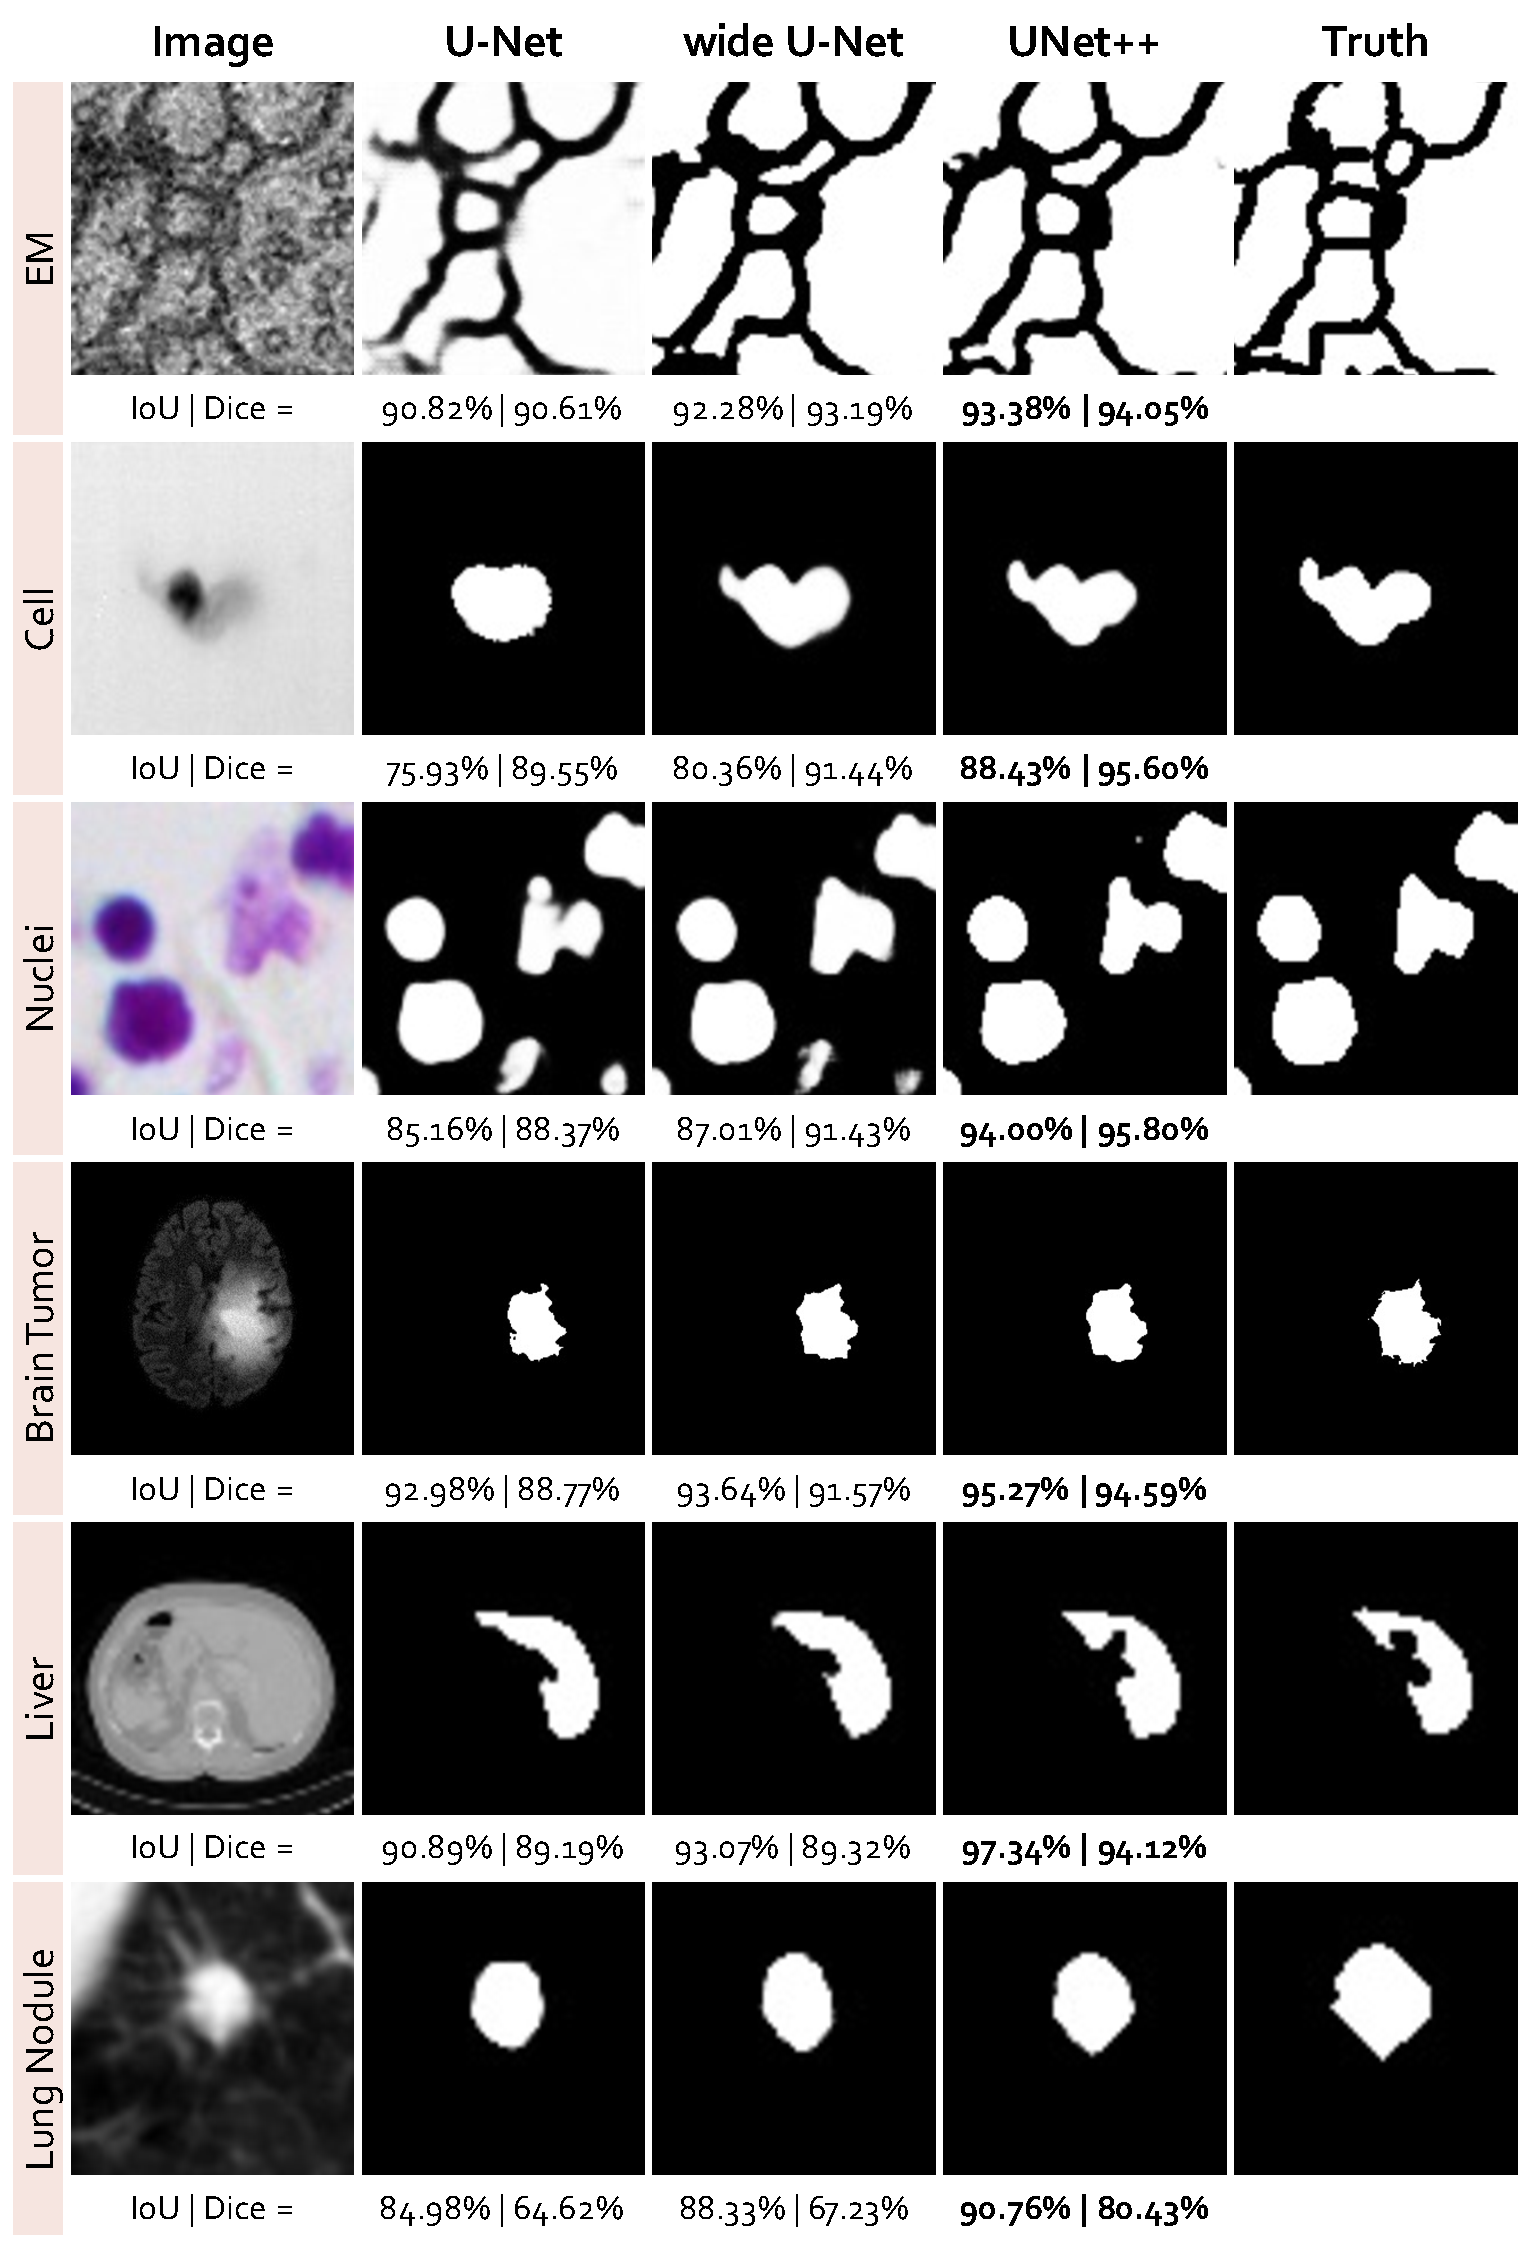
\includegraphics[width=0.6\linewidth]{Figures/CH4/fig_qualitative_comparison.pdf}
\end{center}
\caption[Qualitative Comparison among U-Net, Wide U-Net, and UNet++]{
Qualitative comparison among U-Net, wide U-Net, and UNet++; showing segmentation results for our six distinct biomedical image segmentation applications. They include various 2D and 3D modalities. The corresponding quantitative scores are provided at the bottom of each prediction (IoU $|$ Dice).}
\label{ch4:fig:predict_visualization}
\end{figure}
%##############################################################################################


%##############################################################################################
\begin{table}[t]
\footnotesize
\begin{center}
\begin{threeparttable}
    \caption[Mask RCNN++ Surpasses Mask R-CNN in Instance Segmentation]{
    Redesigned skip connections improve both semantic and instance segmentation for the task of nuclei segmentation. We use Mask R-CNN for instance segmentation and U-Net for semantic segmentation in this comparison.}
    \label{ch4:tab:fcn_family_performance}
    \begin{tabular}{P{0.32\linewidth}P{0.18\linewidth}P{0.12\linewidth}P{0.12\linewidth}P{0.12\linewidth}}
    \hline
     \textbf{Architecture} & \textbf{Backbone} & \textbf{IoU} & \textbf{Dice} & \textbf{Score} \\
    \hline
    U-Net &resnet101&91.03 & 75.73 & 0.244 \\
    \rowcolor{maroon!15}
     UNet++&resnet101&   \bd{92.55} & \bd{89.74} & \bd{0.327} \\
    \hline
    Mask-RCNN &resnet101& 93.28 & 87.91 & 0.401 \\
    \rowcolor{maroon!15}
    MaskRCNN++ &resnet101&\bd{95.10} & \bd{91.36} & \bd{0.414} \\
    \hline
    \end{tabular}
    \begin{tablenotes}
        \scriptsize
        \item[1] Mask R-CNN with UNet++ design in its feature pyramid.
    \end{tablenotes}
\end{threeparttable}
\end{center}
\end{table}
%##############################################################################################


\subsection{MaskRCNN++ Tops Mask-RCNN in Instance Segmentation}
\label{ch4:instance_segmentation}

Instance segmentation consists in segmenting and distinguishing all object instances; hence, more challenging than semantic segmentation. We use Mask R-CNN~\citep{he2017mask} as the baseline model for instance segmentation. Mask R-CNN utilizes feature pyramid network (FPN) as backbone to generate object proposal at multiple scales, and then outputs the segmentation masks for the collected proposals via a dedicated segmentation branch. We modify Mask R-CNN by replacing the plain skip connections of FPN with the redesigned skip connections of UNet++. We refer to this model as Mask RCNN++. We use resnet101 as the backbone for Mask R-CNN in our experiments. 

\tableautorefname~\ref{ch4:tab:fcn_family_performance} compares the performance of Mask R-CNN and Mask RCNN++ for nuclei segmentation.
We have chosen the \texttt{Nuclei} dataset because multiple nucleolus instances can be present in an image, in which case each instance is annotated in a different color, and thus marked as a distinct object. Therefore, this dataset is amenable to both semantic segmentation where all nuclei instances are treated as foreground class, and also instance segmentation where each individual nucleus is to be segmented separately.
As seen in \tableautorefname~\ref{ch4:tab:fcn_family_performance}, Mask RCNN++ outperforms its original counterpart, achieving 1.82 points increase in IoU (93.28\% to 95.10\%), 3.45 points increase in Dice (87.91\% to 91.36\%), and 0.013 points increase in the leaderboard score (0.401 to 0.414). To put this performance in perspective, we have also trained a U-Net and UNet++ model for semantic segmentation with a resnet101 backbone. As seen in \tableautorefname~\ref{ch4:tab:fcn_family_performance}, Mask R-CNN models achieve higher segmentation performance than semantic segmentation models. Furthermore, as expected, UNet++ outperforms U-Net for semantic segmentation.

%##############################################################################################
\begin{figure}[t]
\begin{center}
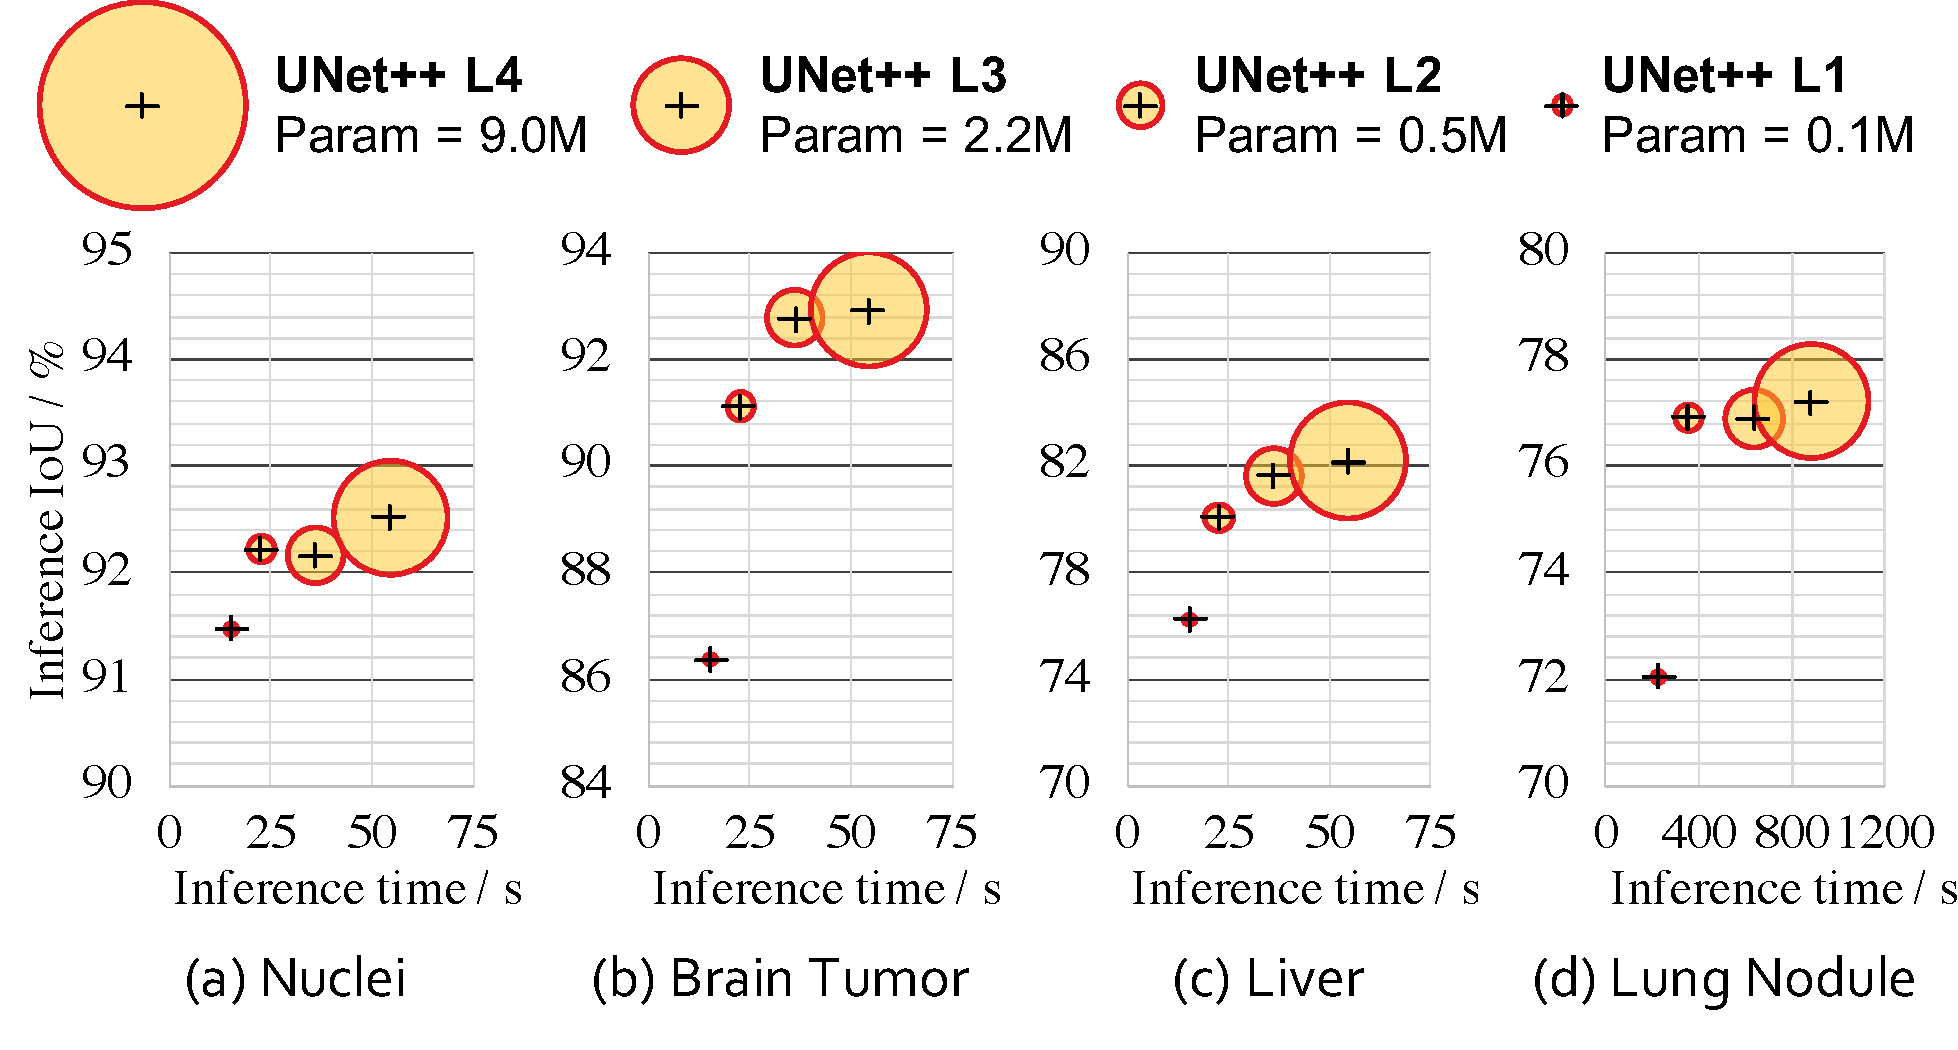
\includegraphics[width=0.8\linewidth]{Figures/CH4/fig_inference_time.pdf}
\end{center}
\caption[UNet++ Accelerates Inference Speed by Model Pruning]{
Complexity (size $\propto$ parameters), inference time, and IoU of UNet++ under different levels of pruning. The inference time is calculated by the time taken to process 10K test images on a single NVIDIA TITAN X (Pascal) GPU with 12 GB memory.}
\label{ch4:fig:speed_accuracy}
\end{figure}
%##############################################################################################



\subsection{UNet++ Accelerates Inference Speed by Model Pruning}
\label{ch4:model_pruning}

Once UNet++ is trained, the decoder path for depth $d$ at inference time is completely independent from the decoder path for depth $d+1$. As a result, we can completely remove the decoder for depth $d+1$, obtaining a shallower version of the trained UNet++ at depth $d$, owing to the introduced deep supervision. This pruning can significantly reduce the inference time, but segmentation performance may degrade. As such, the level of pruning should be determined by evaluating the model's performance on the validation set. We have studied the inference speed-IoU trade-off for UNet++ in \figurename~\ref{ch4:fig:speed_accuracy}. We use UNet++ L$d$ to denote UNet++ pruned at depth $d$ (see \figurename~\ref{ch4:fig:prune_structure} for further details). As seen, UNet++ L${3}$ achieves on average 32.2\% reduction in inference time and 75.6\% reduction in memory footprint while degrading IoU by only 0.6 points. More aggressive pruning further reduces the inference time but at the cost of significant IoU degradation. More importantly, this observation has the potential to exert important impact on computer-aided diagnosis (CAD) on mobile devices, as the existing deep convolutional neural network models are computationally expensive and memory intensive.

%##############################################################################################
\begin{figure}[t]
\begin{center}
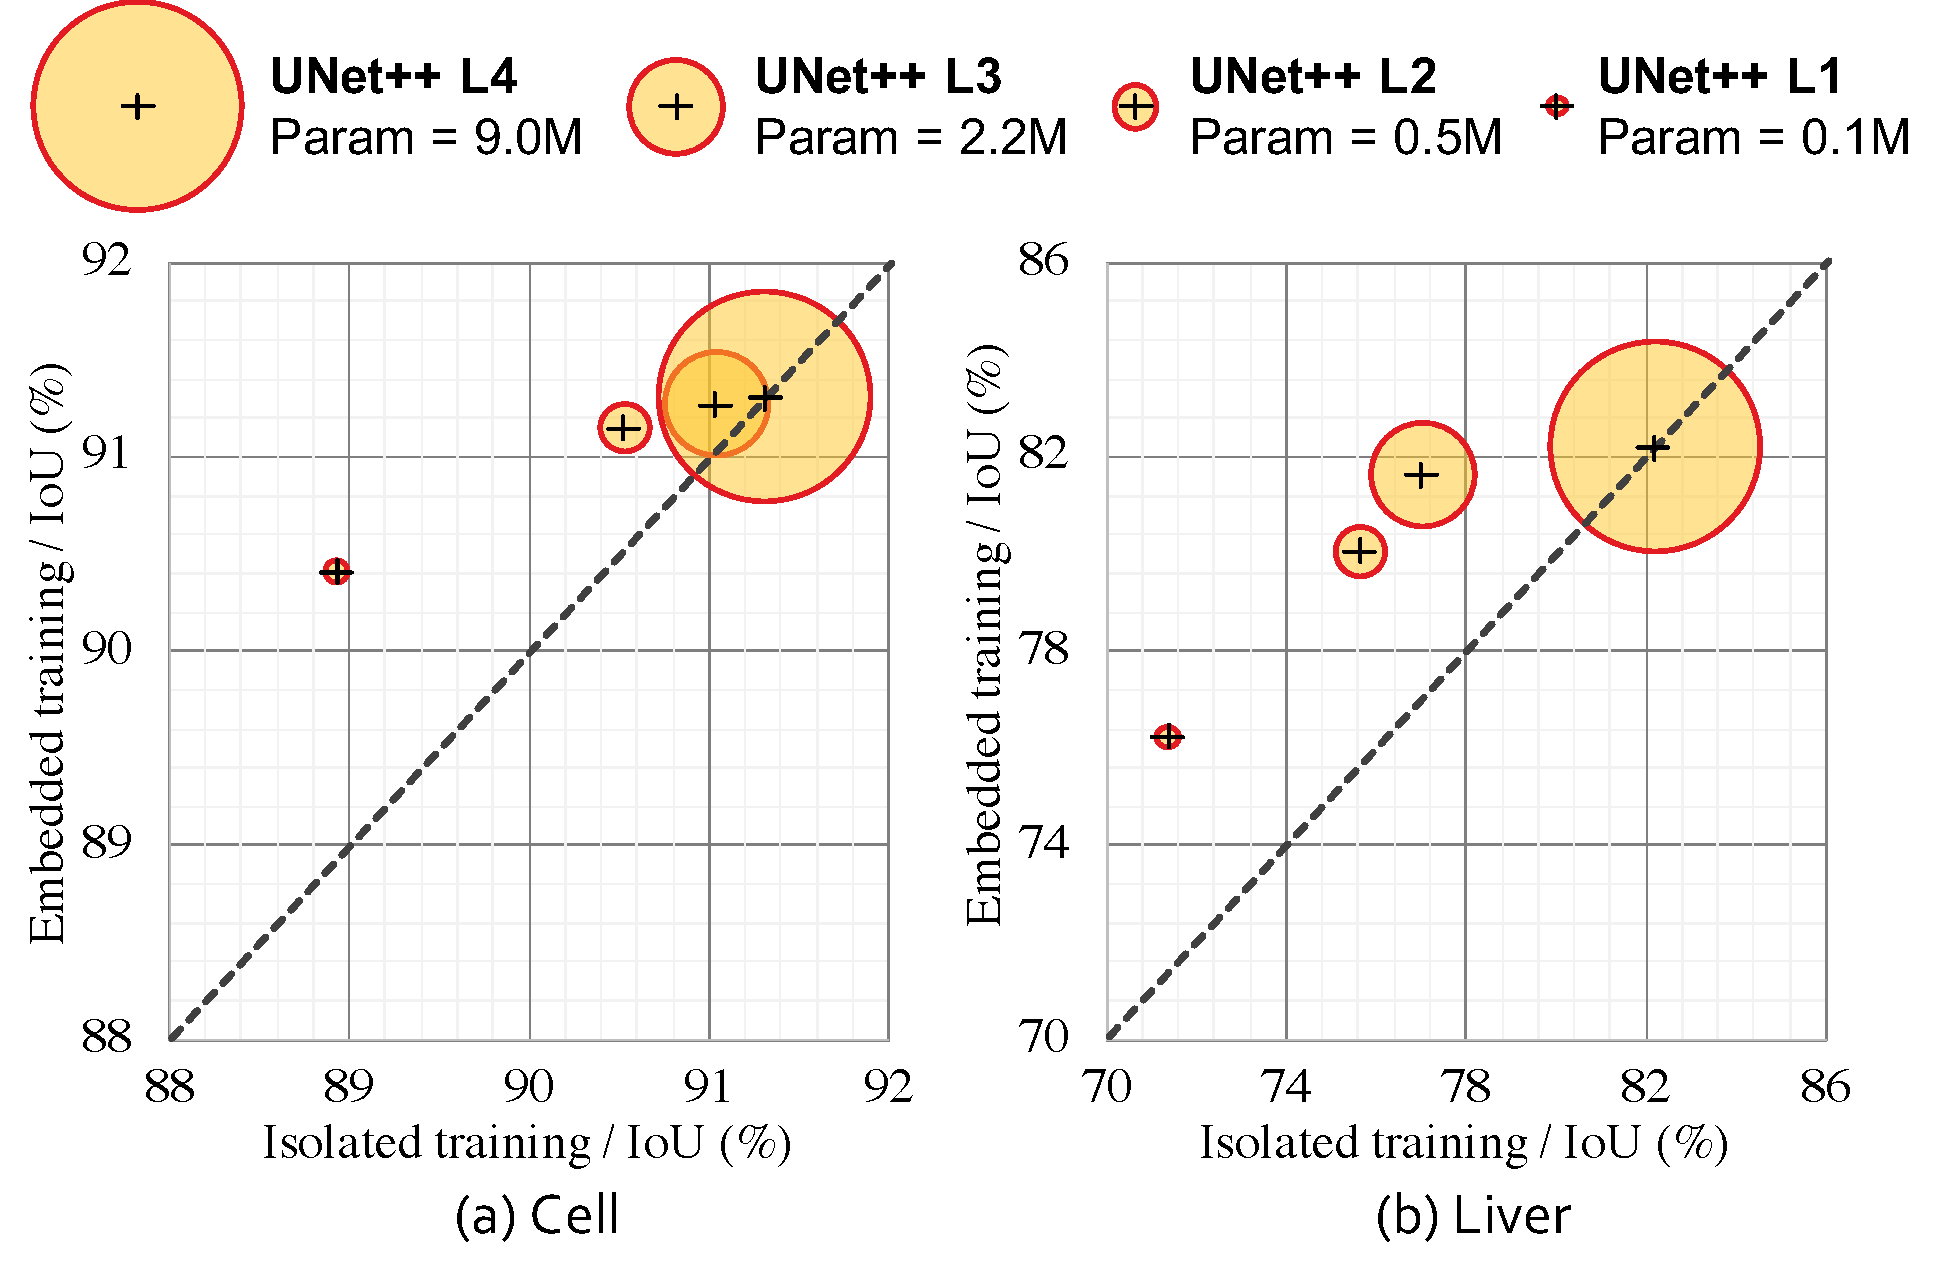
\includegraphics[width=0.8\linewidth]{Figures/CH4/fig_isolated_embedded.pdf}
\end{center}
\caption[Embedded UNet++ Surpasses Isolated U-Nets]{
We demonstrate that our architectural design improves the performance of each shallower network embedded in UNet++. The embedded shallower networks show improved segmentation when pruned from UNet++ in comparison to the same network trained isolated. Due to no pruning, UNet++ L$4$ naturally achieves the same level of performance in isolated and embedded training modes.}
\label{ch4:fig:pruned_vs_stand-alone}
\end{figure}
%##############################################################################################



\subsection{Embedded UNet++ Surpasses Isolated U-Nets}
\label{ch4:embedded_vs_isolated_training}

In theory, UNet++ L$d$ can be trained in two fashions: 1) embedded training where the full UNet++ model is trained and then pruned at depth $d$ to obtain UNet++ L$d$, 2) isolated training where UNet++ L$d$ is trained in isolation without any interactions with the deeper encoder and decoder nodes. Referring to~\figurename~\ref{ch4:fig:prune_structure}, embedded training of a sub-network consists of training all graph nodes (both yellow and grey components) with deep supervision, but we then use only the yellow sub-network during the inference time. In contrast, isolated training consists of removing the grey nodes from the graph, basing the training and test solely on the yellow sub-network.

We have compared the isolated and embedded training schemes for various levels of UNet++ pruning across two datasets in~\figurename~\ref{ch4:fig:pruned_vs_stand-alone}\footnote{I thank Mohammad Reza Hosseinzadeh Taher and Fatemeh Haghighi for their verification of liver segmentation performance and the ablation study of embedded and isolated UNet++.}. We have discovered that the embedded training of UNet++ L$d$ results in a higher performing model than training the same architecture in isolation. The observed superiority is more pronounced under aggressive pruning when the full UNet++ is pruned to UNet++ L$1$. In particular, the embedded training of UNet++ L$1$ for liver segmentation achieves 5-point increase in IoU over the isolated training scheme. This finding suggests that supervision signal coming from the deep downstream enables training higher performing shallower models. This finding is also related to knowledge distillation where the knowledge learned by a deep teacher network is learned by a shallower student network.

%##############################################################################################
\begin{figure}[t]
\begin{center}
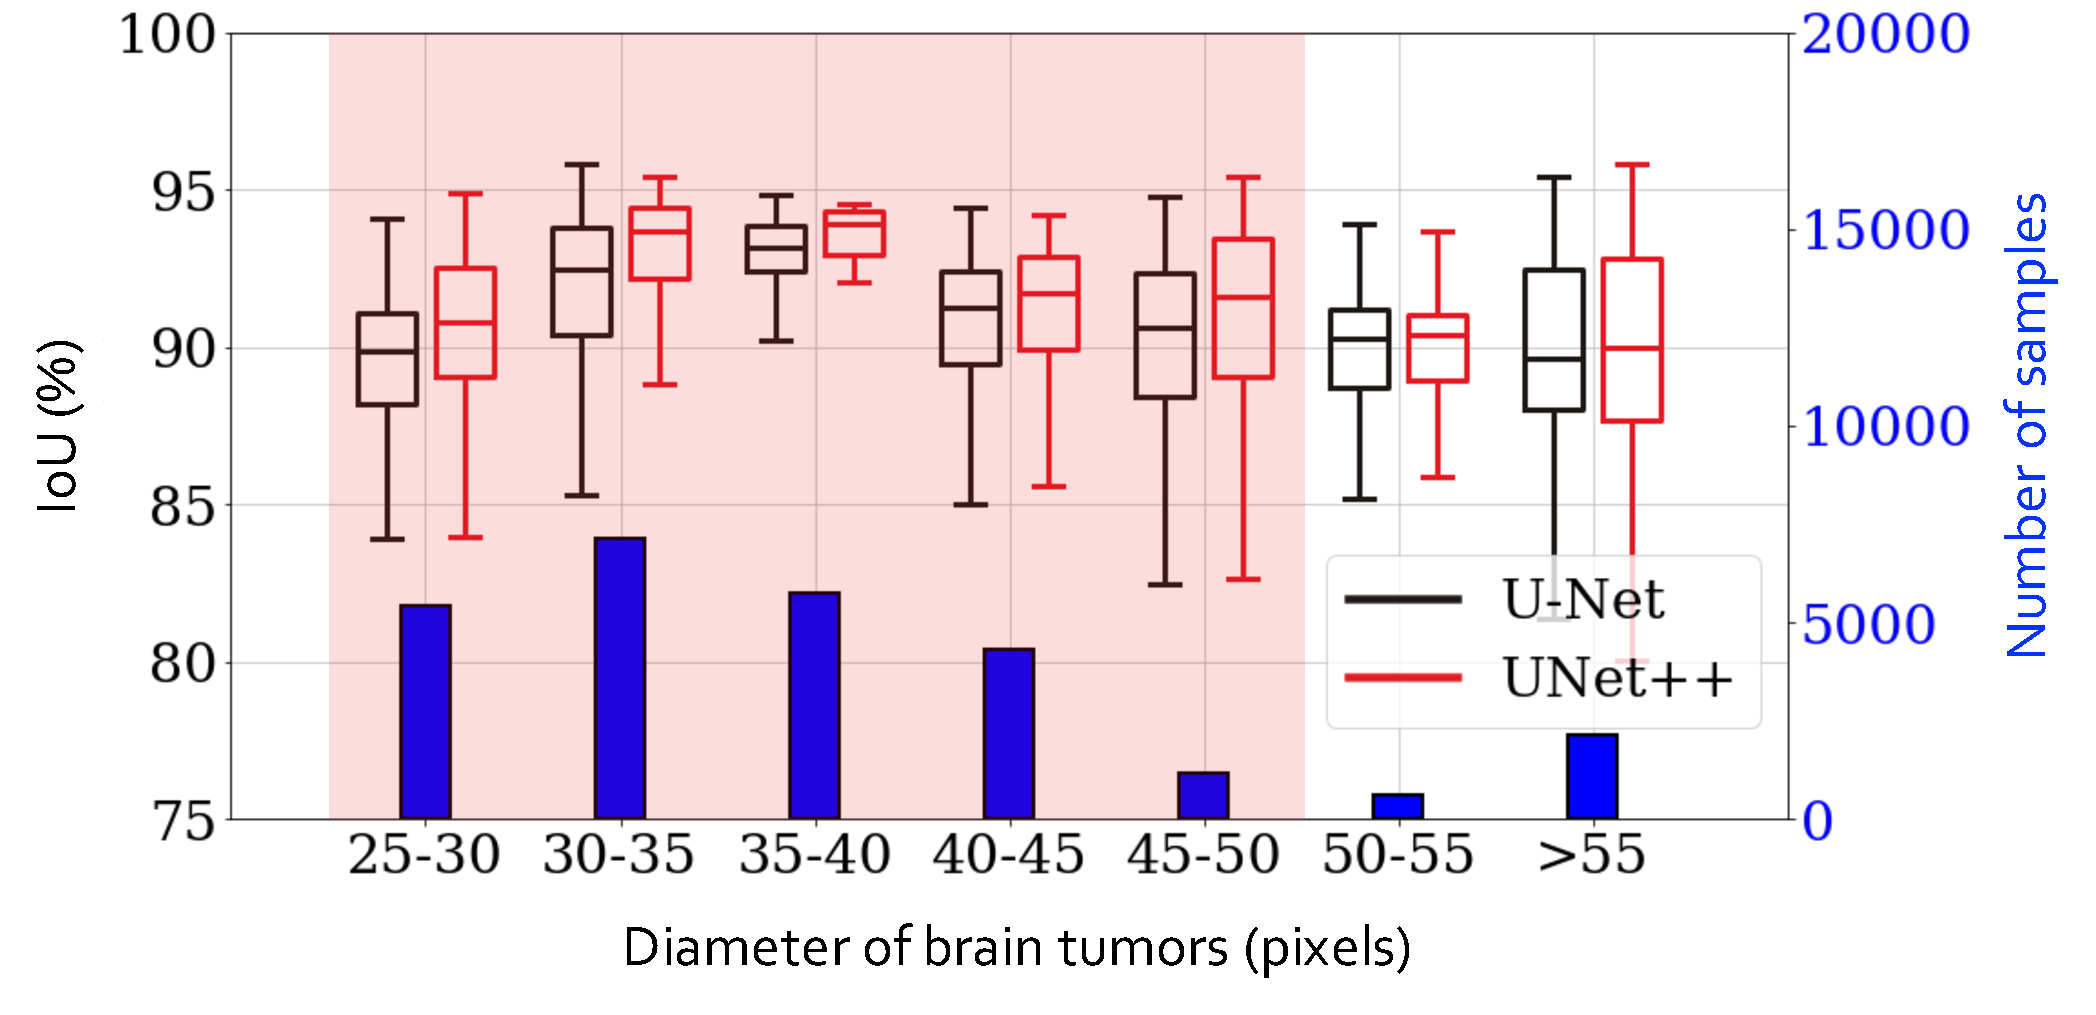
\includegraphics[width=0.85\linewidth]{Figures/CH4/fig_physical_real_brain_tumor_size_stat.pdf}
\end{center}
\caption[UNet++ Can Segment Lesions with Varying Sizes]{
UNet++ can better segment tumors of various sizes than does U-Net. We measure the size of tumors based on the ground truth masks and then divide them into seven groups. The histogram shows the distribution of different tumor sizes. The box-plot compares the segmentation performances of U-Net (black) and UNet++ (red) in each group. The $t$-test for two independent samples has been further performed on each group. As seen, UNet++ improves segmentation for all sizes of tumors and the improvement is significant ($p<0.05$) for the majority of the tumor sizes (highlighted in red).}
\label{ch4:fig:multi_depth_improvement_brain_tumor}
\end{figure}
%##############################################################################################


\section{Discussion \& Conclusion}
\label{ch4:discussion_conclusion}


\subsection{Can UNet++ Segment Lesions with Varying Sizes?}
\label{ch4:discussion_conclusion:stratified_lesion_sizes}

\figurename~\ref{ch4:fig:multi_depth_improvement_brain_tumor} compares U-Net and UNet++ for segmenting different sizes of brain tumors. To avoid clutter in the figure, we group the tumors by size into seven buckets. As seen, UNet++ consistently outperforms U-Net across all the buckets. We also adopt $t$-test on each bucket based on 20 different trials to measure the significance of the improvement, concluding that 5 out of the 7 comparisons are statistically significant ($p < 0.05$). The capability of UNet++ in segmenting tumors of varying sizes is attributed to its built-in ensemble of U-Nets, which enables image segmentation based on multi-receptive field networks.

%##############################################################################################
% \begin{landscape}
% \thispagestyle{empty}

\begin{sidewaysfigure}
\begin{center}
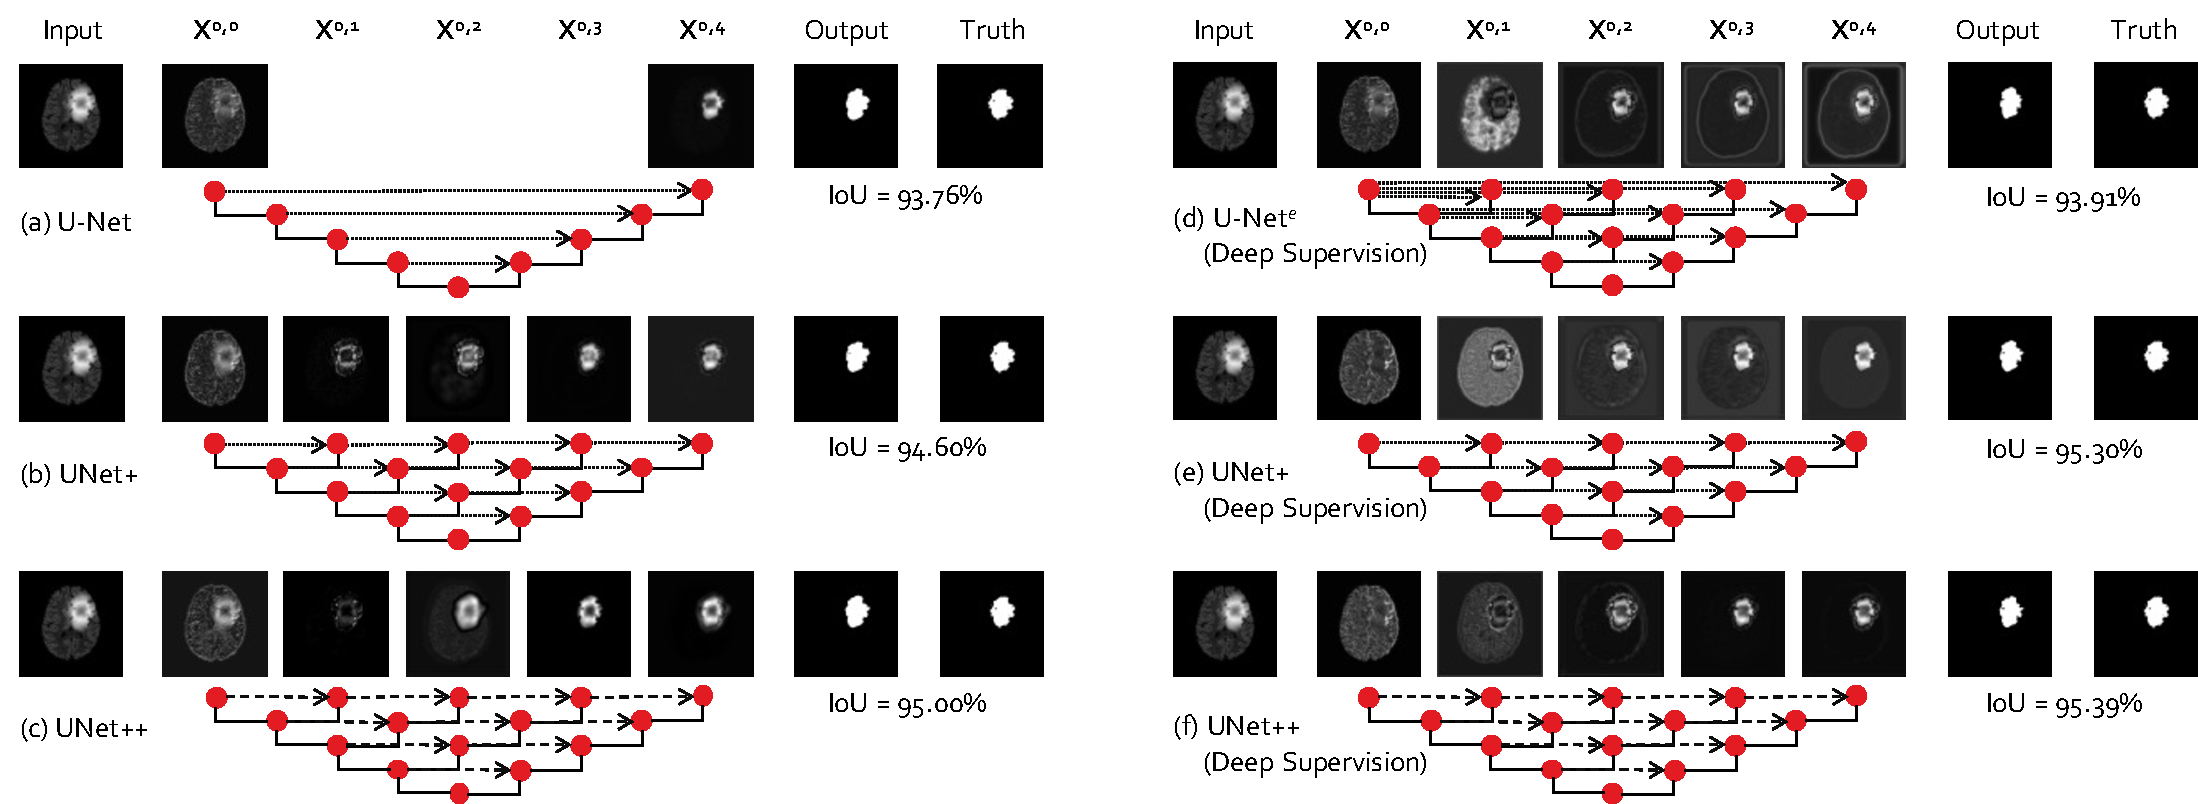
\includegraphics[width=1.0\columnwidth]{Figures/CH4/fig_feature_map_aggregation_brats.pdf}
\end{center}
\caption[Visualization of Multi-scale Feature Map Aggregation]{Visualization and comparison of feature maps from early, intermediate, and late layers along the top most skip connection for brain tumor images. Here, the dot arrows denote the plain skip connection in U-Net and UNet+, while the dash arrows denote dense connections introduced in UNet++.}
\label{ch4:fig:feature_map_aggregation}
\end{sidewaysfigure}

% \fillandplacepagenumber
% \end{landscape}
%##############################################################################################


%##############################################################################################
\begin{figure}[t]
\begin{center}
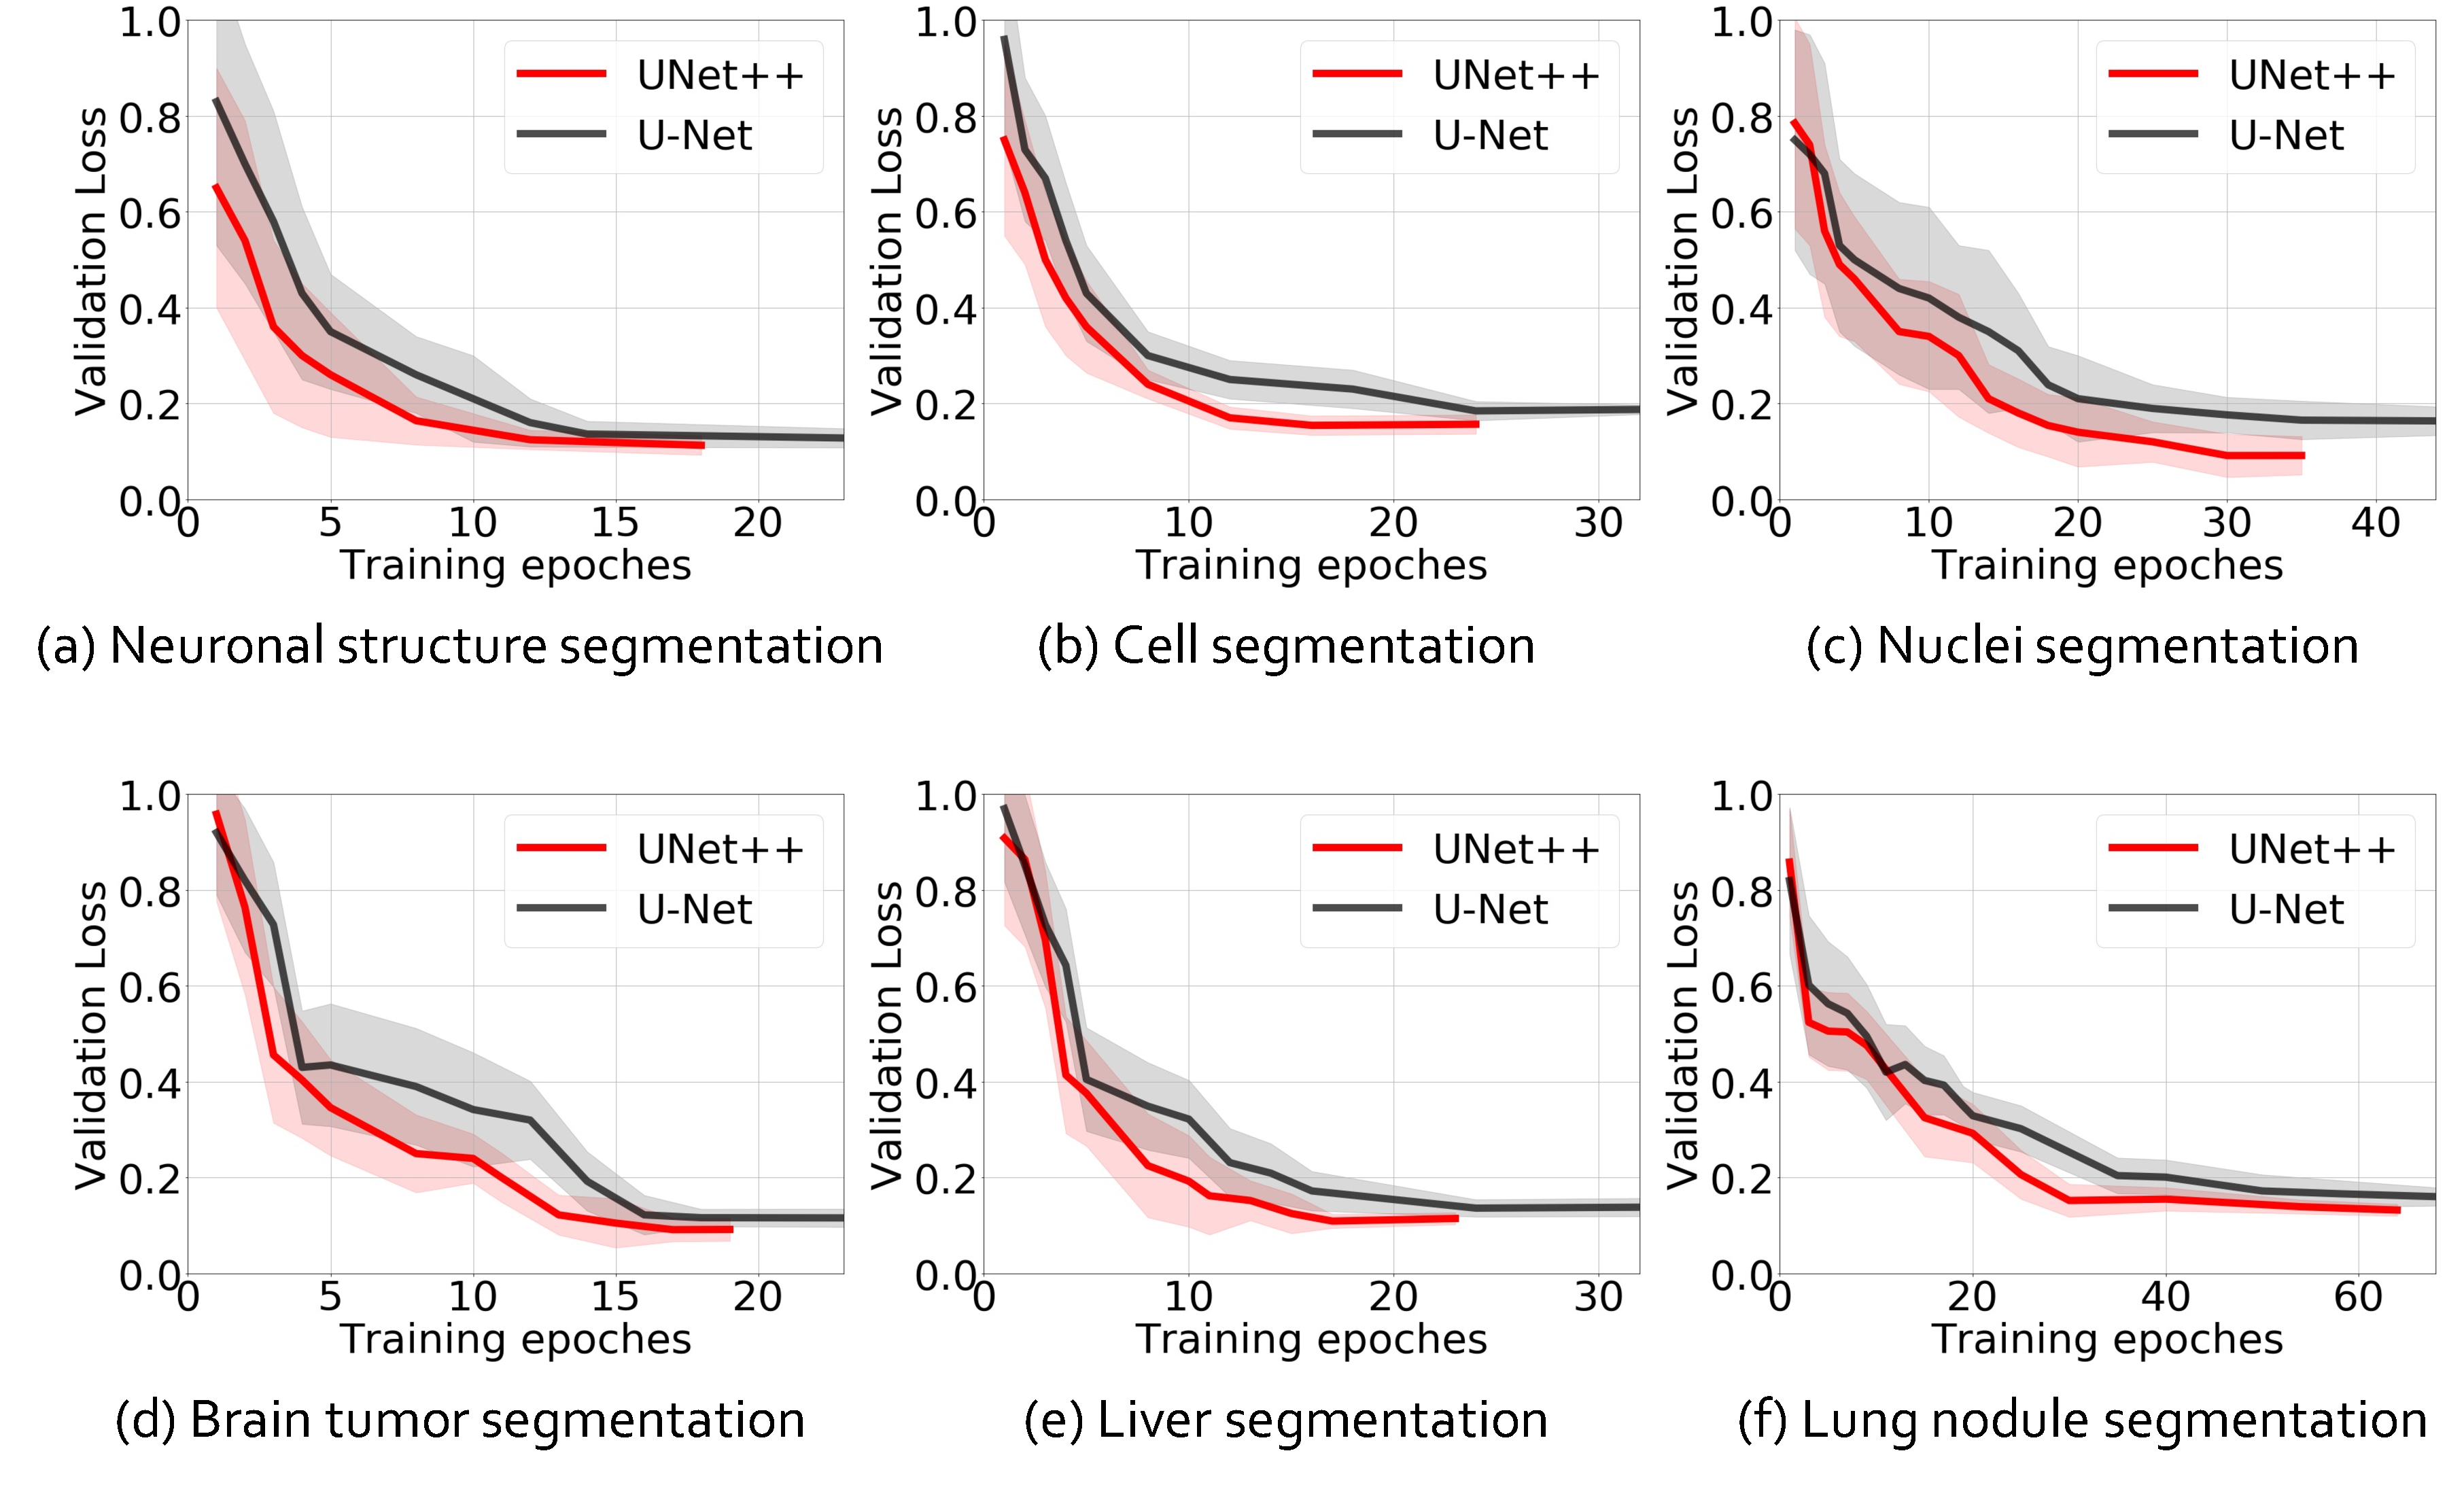
\includegraphics[width=1.0\linewidth]{Figures/CH4/fig_learning_curves.pdf}
\end{center}
\caption[UNet++ Enables a Better Optimization than U-Net]{
UNet++ enables a better optimization than U-Net evidenced by the learning curves for the tasks of neuronal structure, cell, nuclei, brain tumor, liver, and lung nodule segmentation. We have plotted the validation losses averaged by 20 trials for each application. As seen, UNet++ with deep supervision accelerates the convergence speed and yields the lower validation loss due to the new design of the intermediate layers and dense skip connections.}
\label{ch4:fig:learning_curves}
\end{figure}
%##############################################################################################



\subsection{How Do Multi-scale Feature Maps Aggregate in UNet++?}
\label{ch4:discussion_conclusion:feature_maps_visualization}

In Section~\ref{ch4:motiv}, we explained that the redesigned skip connections enable the fusion of semantically rich decoder feature maps with feature maps of varying semantic scales from the intermediate layers of the architecture. In this section, we illustrate this privilege of our re-designed skip connections by visualizing the intermediate feature maps.

\figurename~\ref{ch4:fig:feature_map_aggregation} shows representative feature maps from early, intermediate, and late layers along the top most skip connection (\ie X$^{0,i}$) for a brain tumor image. The representative feature map for a layer is obtained by averaging all its feature maps. Also note that architectures in the left side of \figurename~\ref{ch4:fig:feature_map_aggregation} are trained using only loss function appended to the deepest decoder layer (X$^{0,4}$) whereas the architectures in the right side of \figurename~\ref{ch4:fig:feature_map_aggregation} are trained with deep supervision. 
Note that these feature maps are not the final outputs. We have appended an additional 1$\times$1 convolutional layer on top of each decoder branch to form the final segmentation.
We observe that the outputs of U-Net's intermediate layers are semantically dissimilar  whereas for UNet+ and UNet++ the outputs are formed gradually. The output of node X$^{0,0}$ in U-Net undergoes slight transformation (few convolution operations only) whereas the output of X$^{1,3}$, the input of X$^{0,4}$, goes through nearly every transformation (four down-sampling and three up-sampling stages) learned by the network. Hence, there is a large gap between the representation capability of X$^{0,0}$ and X$^{1,3}$. So, simply concatenating the outputs of X$^{0,4}$ and X$^{1,3}$ is not an optimal solution. In contrast, redesigned skip connections in UNet+ and UNet++ help refine the segmentation result gradually. 
We further present the learning curves of all six medical applications in~\figurename~\ref{ch4:fig:learning_curves}, revealing that the addition of dense connections in UNet++ encourages a better optimization and reaches lower validation loss.


\subsection{Isolated Learning or Collaborative Learning?}
\label{ch4:discussion_conclusion:collarborative_learning}

Collaborative learning is known as training multiple classifier heads of the same network simultaneously on the same training data. It is found to improve the generalization power of deep neural networks~\citep{song2018collaborative}. UNet++ naturally embodies collaborative learning through aggregating multi-depth networks and supervising segmentation heads from each of the constituent networks. Besides, the segmentation heads, for example X$^{0,2}$ in \figurename~\ref{ch4:fig:prune_structure}, receive gradients from both strong (loss from ground truth) and soft (losses propagated from adjacent deeper nodes) supervision. As a result, the shallower networks improve their segmentation (\figurename~\ref{ch4:fig:pruned_vs_stand-alone}) and provide more informative representation to deeper counterparts. Basically, deeper and shallower networks regularize each other via collaborative learning in UNet++. Training multi-depth embedded networks together results in improved segmentation than training them individually as isolated network which is evident in \sectionname~\ref{ch4:embedded_vs_isolated_training}. The embedded design of UNet++ makes it amenable to auxiliary training, multi-task learning, and knowledge distillation~\citep{bengio2009learning,hinton2015distilling,song2018collaborative}.

% \subsection{Can UNet++ facilitate active learning in segmentation?}
% \label{ch4:discussion_conclusion:unetplusplus_active_learning_segmentation}


\subsection{Conclusion and Broader Impacts}
\label{ch4:discussion_conclusion:conclusion_broader_impacts}

We have presented a novel architecture, named UNet++, for more accurate image segmentation. The improved performance by our UNet++ is attributed to its nested structure and re-designed skip connections, which aim to address two key challenges of the U-Net: 1) unknown depth of the optimal architecture and 2) the unnecessarily restrictive design of skip connections. We have evaluated UNet++ using six distinct biomedical imaging applications and demonstrated consistent performance improvement over various state-of-the-art backbones for semantic segmentation and meta framework for instance segmentation.

We first presented UNet++ in our DLMIA 2018 paper~\citep{zhou2018unet++}. 
UNet++ has since been widely adopted by the research community, either as a strong baseline for comparison~\citep{sun2019high,fang2019selective,fang2019improved,meng2020multiscale}, or as a source of inspiration for developing newer semantic segmentation architectures~\citep{zhang2018mdu,chen2018improved,zhou2018learning,wu2019automatical,song2019u,yang2019eda}; it has also been utilized for multiple applications, not only for diseases/organs/tissues segmentation in biomedical images~\citep{zyuzin2019comparison,cui2019pulmonary}, but also for image coloring~\citep{di2021color}, moon impact crater detection~\citep{jia2021moon}, microseismic monitoring~\citep{guo2021first}. Recently, \citet{shenoy2019feature} has independently and systematically investigated UNet++ for the task of ``contact prediction model PconsC4'', demonstrating significant improvement over widely-used U-Net. 



% \section*{Acknowledgements}

% I thank Mohammad Reza Hosseinzadeh Taher and Fatemeh Haghighi for their verification of liver segmentation performance and the ablation study of embedded and isolated UNet++. I also thank Michael G. Meyer for allowing us to test our ideas on the Cell-CT dataset.
\chapter{Extracting Features from Unannotated Images}
\label{ch5}

This chapter is based on the following publications:
\begin{itemize}
    \item Zhou, Z., Sodha, V., Rahman Siddiquee M. M., Feng, R., Tajbakhsh, N., Gotway, M. B., \& Liang, J. (2019, October). Models genesis: Generic autodidactic models for 3d medical image analysis. In \textit{International Conference on Medical Image Computing and Computer-Assisted Intervention} (pp. 384-393). Springer, Cham.
    \item Zhou, Z., Sodha, V., Pang, J., Gotway, M. B., \& Liang, J. (2021). Models genesis. \textit{Medical image analysis}, 67, 101840.
\end{itemize}

% \section*{CRediT authorship contribution statement}

% I would like to thank all of the authors for their contributions and hard works. Vatsal Sodha: software, investigation, visualization. Jiaxuan Pang: software, investigation. Michael B. Gotway: resources, data curation, funding acquisition. Jianming Liang: conceptualization, methodology, formal analysis, investigation, resources, writing, supervision, project administration, funding acquisition. 

\newpage

\section{Background \& Motivation}

Recent years have featured a trend towards pre-trained image representations in computer vision, applied in increasingly flexible and task-agnostic ways for downstream transfer.
Transfer learning from {\em natural} images to {\em medical} images has become the \textit{de facto} standard in deep learning for medical image analysis~\citep{tajbakhsh2016convolutional,shin2016deep}, but given the marked differences between {\em natural} images and {\em medical} images, we hypothesize that transfer learning can yield more powerful (application-specific) {\em target} models from the {\em source} models built directly using medical images. To test this hypothesis, we have chosen chest imaging because the chest contains several critical organs, which are prone to a number of diseases that result in substantial morbidity and mortality, hence associated with significant health-care costs. In this research, we focus on Chest CT, because of its prominent role in diagnosing lung diseases, and our research community has accumulated several Chest CT image databases, for instance, LIDC-IDRI~\citep{armato2011lung} and NLST~\citep{national2011reduced}, containing a large number of Chest CT images. However, systematically annotating Chest CT scans is not only tedious, laborious, and time-consuming, but it also demands costly, specialty-oriented skills, which are not easily accessible. Therefore, we seek to answer the following question: {\em Can we utilize the large number of available Chest CT images without systematic annotation to train source models that can yield high-performance target models via transfer learning?} 

To answer this question, we have developed a framework that trains generic source models for 3D medical imaging. Our framework is {\em autodidactic}---eliminating the need for labeled data by self-supervision; {\em robust}---learning comprehensive image representation from a mixture of self-supervised tasks; {\em scalable}---consolidating a variety of self-supervised tasks into a single image restoration task with the same encoder-decoder architecture; and {\em generic}---benefiting a range of 3D medical imaging tasks through transfer learning.
We call the models trained with our framework Generic Autodidactic Models, nicknamed Models Genesis, and refer to the model trained using Chest CT images as Genesis Chest CT.
As ablation studies, we have also trained a downgraded 2D version using 2D Chest CT slices, called Genesis Chest CT 2D. For thorough performance comparisons, we have trained a 2D model using Chest X-ray images, named as Genesis Chest X-ray (detailed in~\tablename~\ref{ch5:tab:terminology}). 

Naturally, 3D imaging tasks in the most prominent medical imaging modalities (\eg CT and MRI) should be solved directly in 3D, but 3D models generally have significantly more parameters than their 2D counterparts, thus demanding more labeled data for training. As a result, learning from scratch simply in 3D may {\em not} necessarily yield performance better than fine-tuning Models ImageNet (\ie pre-trained models on ImageNet), as revealed in \figurename~\ref{ch5:fig:2D_3D_target_tasks}. However, as demonstrated by our extensive experiments in Sec.~\ref{ch5:experiments}, our Genesis Chest CT not only {\em significantly} outperforms learning 3D models from scratch (see \figurename~\ref{ch5:fig:random_initialization}), but also {\em consistently} tops any 2D/2.5D approaches including fine-tuning Models ImageNet as well as fine-tuning our Genesis Chest X-ray and Genesis Chest CT 2D (see \figurename~\ref{ch5:fig:2D_3D_target_tasks} and \tablename~\ref{ch5:tab:3d_2.5d_2d}). Furthermore, Genesis Chest CT surpasses publicly-available, pre-trained, (fully) supervised 3D models (see \tablename~\ref{ch5:tab:top_existing_models}). Our results  confirm the importance of 3D anatomical information and demonstrate the significance of Models Genesis for 3D medical imaging.

This performance is attributable to the following key observation: medical imaging protocols typically focus on particular parts of the body for specific clinical purposes, resulting in images of similar anatomy. The sophisticated yet recurrent anatomy offers consistent patterns for self-supervised learning to discover common representation of a particular body part (the lungs in our case). 
As illustrated in \figurename~\ref{ch5:fig:self_supervised_learning_framework}, the fundamental idea behind our self-supervised learning method is to recover anatomical patterns from images transformed via various ways in a unified framework. 

In summary, we make the following three contributions:
\begin{enumerate}
    \item A collection of generic pre-trained 3D models, performing effectively across diseases, organs, and modalities.
    \item A scalable self-supervised learning framework, offering encoder for classification and encoder-decoder for segmentation.
    \item A set of self-supervised training schemes, learning robust representation from multiple perspectives.
\end{enumerate}


%%%%%%%%%%%%%%%%%%%%%%%%%%%%%%%%%%%%%%%%%%%%
% \begin{landscape}
% \thispagestyle{empty}

\begin{sidewaystable}
\begin{threeparttable}[t]
\begin{center}
\footnotesize
\caption[Definition of Pre-trained Models, Proxy and Target Tasks]{
% Pre-trained models with proxy tasks and target tasks. 
We use transfer learning in a broader sense, where a \textit{source model} is first trained to learn image presentation via \textit{full supervision} or \textit{self supervision} by solving a problem, called \textit{proxy task} (general or application-specific), on a \textit{source dataset} with \textit{expert-provided} or \textit{automatically-generated} labels, and then this \textit{pre-trained} source model is fine tuned (transferred) through full supervision to yield a \textit{target model} to solve application-specific problems (\textit{target tasks}) in the same or different datasets (\textit{target datasets}). 
% We refer transfer learning to \textit{same-domain} transfer learning when the models are pre-trained and fine-tuned within the same domain (modality, organ, disease, or dataset), and to \textit{cross-domain} when the models are pre-trained in one domain and fine-tuned for a different domain.
  }
\label{ch5:tab:terminology}
    \begin{tabular}{p{0.04\linewidth}p{0.14\linewidth}p{0.07\linewidth}p{0.16\linewidth}p{0.13\linewidth}p{0.32\linewidth}}
        \hline
        \multicolumn{2}{l}{Pre-trained model} & Modality & Source dataset & Superv. / Annot. & Proxy task  \\
        \hline
        \multicolumn{2}{l}{Genesis Chest CT 2D} & CT & LUNA~2016 & Self / 0 & Image restoration on 2D Chest CT slices \\
        \multicolumn{2}{l}{Genesis Chest CT (3D)} & CT & LUNA~2016 & Self / 0 & Image restoration on 3D Chest CT volumes \\
        \multicolumn{2}{l}{Genesis Chest X-ray (2D)} & X-ray & ChestX-ray8 & Self / 0 & Image restoration on 2D Chest Radiographs \\
        \multicolumn{2}{l}{Models ImageNet} & Natural & ImageNet & Full / 14M images & Image classification on 2D ImageNet \\
        \multicolumn{2}{l}{Inflated 3D (I3D)} & Natural & Kinetics & Full / 240K videos & Action recognition on human action videos \\
        \multicolumn{2}{l}{NiftyNet} & CT & Pancreas-CT \& BTCV & Full / 90 cases & Organ segmentation on abdominal CT \\
        \multicolumn{2}{l}{MedicalNet} & CT, MRI & 3DSeg-8 & Full / 1,638 cases & Disease/organ segmentation on 8 datasets \\
        \hline
        Code$^{\dagger}$ & Object & Modality & \multicolumn{2}{l}{Target dataset}  & Target task \\
        \hline
        \texttt{NCC} & Lung Nodule & CT & \multicolumn{2}{l}{LUNA~2016~\citep{setio2017validation}} & Lung nodule false positive reduction \\
        \texttt{NCS} & Lung Nodule & CT & \multicolumn{2}{l}{LIDC-IDRI~\citep{armato2011lung}} & Lung nodule segmentation \\
        \texttt{ECC} & Pulmonary Emboli & CT & \multicolumn{2}{l}{PE-CAD~\citep{tajbakhsh2015computer}}  & Pulmonary embolism false positive reduction \\
        \texttt{LCS} & Liver & CT & \multicolumn{2}{l}{LiTS~2017~\citep{bilic2019liver}} & Liver segmentation \\
        \texttt{BMS} & Brain Tumor & MRI & \multicolumn{2}{l}{BraTS~2018~\citep{bakas2018identifying}} & Brain tumor segmentation \\
        \hline
    \end{tabular}
    \begin{tablenotes}
        \scriptsize
        % \item
        \item $^{\dagger}$ The first letter denotes the object of interest (``\texttt{N}'' for lung nodule, ``\texttt{E}'' for pulmonary embolism, ``\texttt{L}'' for liver, etc); the second letter denotes the modality (``\texttt{C}'' for CT, ``\texttt{M}'' for MRI, etc);  the last letter denotes the task (``\texttt{C}'' for classification, ``\texttt{S}'' for segmentation).
    \end{tablenotes}
\end{center}
\end{threeparttable}
\end{sidewaystable}
% }
% \fillandplacepagenumber
% \end{landscape}
%%%%%%%%%%%%%%%%%%%%%%%%%%%%%%%%%%%%%%%%%%%%


%%%%%%%%%%%%%%%%%%%%%%%%%%%%%%%%%%%%%%%%%%%%
% \begin{landscape}
% \thispagestyle{empty}

\begin{sidewaysfigure}
\begin{center}
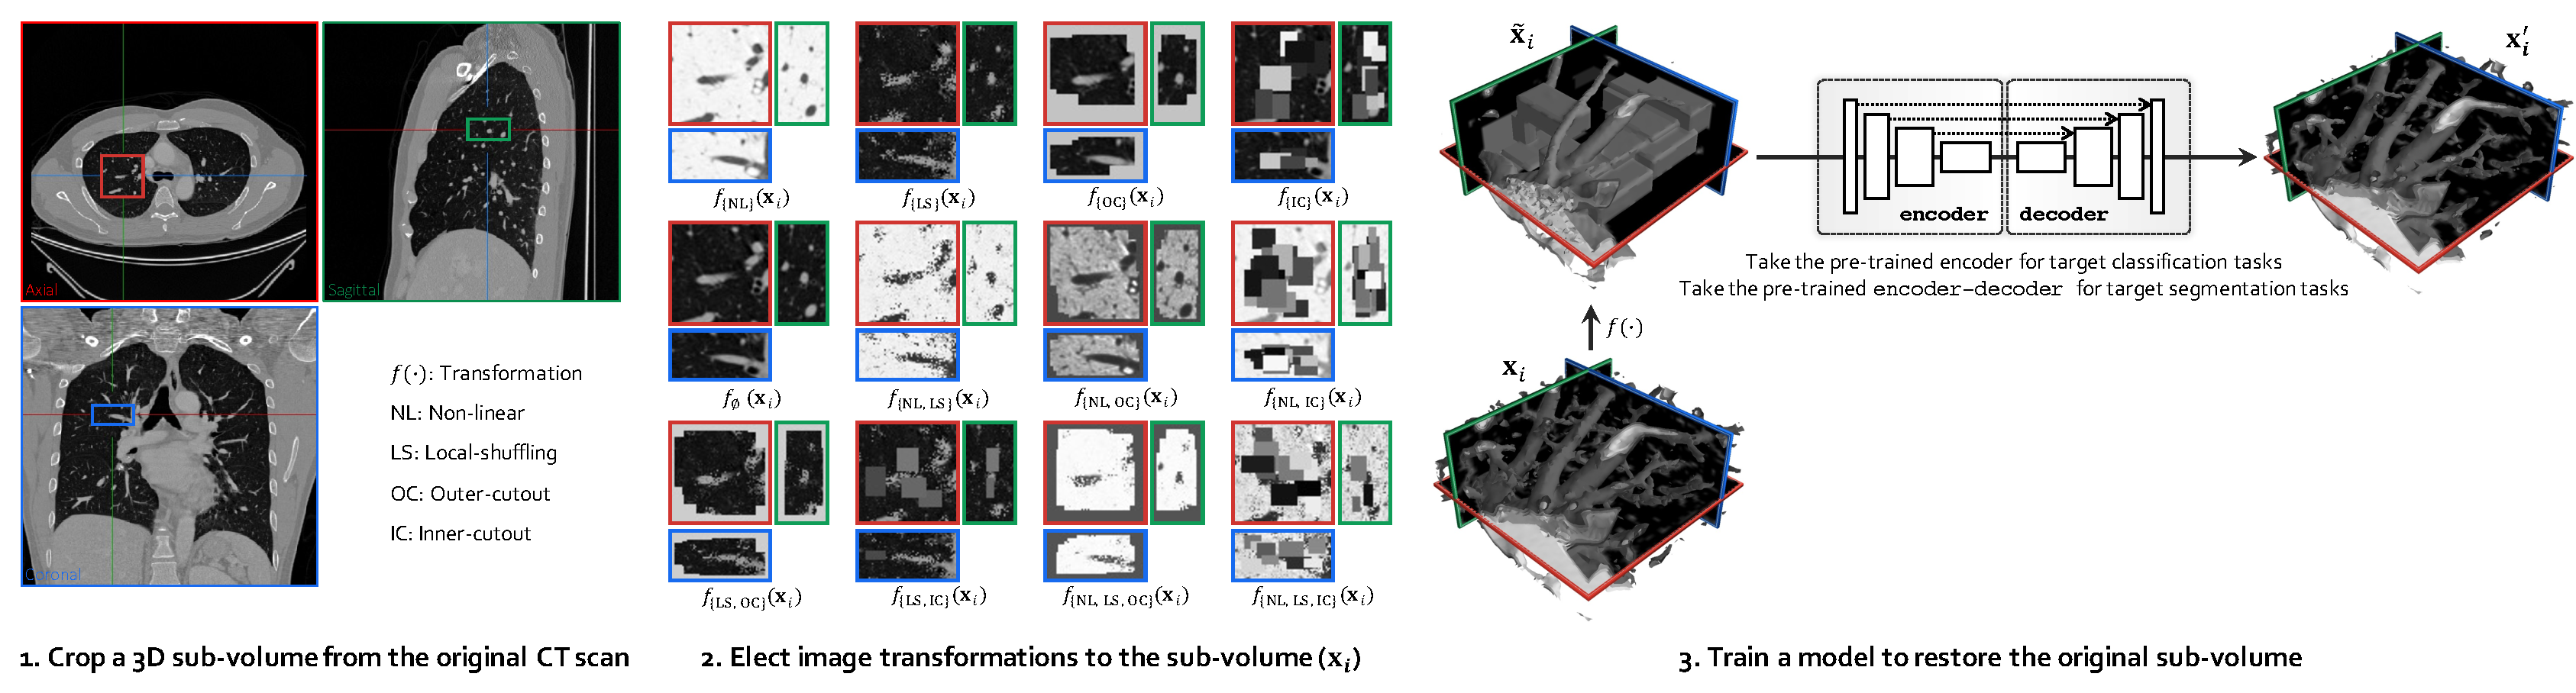
\includegraphics[width=1.0\linewidth]{Figures/CH5/fig_genesis_method.pdf}
\end{center}
\caption[Models Genesis Learn Generic Features by Image Restoration]{
Our self-supervised learning framework aims to learn general-purpose image representation by recovering the original sub-volumes of images from their transformed ones. We first crop arbitrarily-size sub-volume $\textbf{x}_i$ at a random location from an unlabeled CT image. Each sub-volume $\textbf{x}_i$ can undergo at most three out of four transformations: non-linear, local-shuffling, outer-cutout, and inner-cutout, resulting in a transformed sub-volume $\tilde{\textbf{x}}_i$. It should be noted that outer-cutout and inner-cutout are considered mutually exclusive. Therefore, in addition to the four original individual transformations, this process yields eight more transformations, including one identity mapping ($\phi$ meaning none of the four individual transformations is selected) and seven combined transformations. A Model Genesis, an encoder-decoder architecture with skip connections in between, is trained to learn a common image representation by restoring the original sub-volume $\textbf{x}_i$ (as ground truth) from the transformed one $\tilde{\textbf{x}}_i$ (as input), in which the reconstruction loss (MSE) is computed between the model prediction $\textbf{x}_i'$ and ground truth $\textbf{x}_i$. Once trained, the encoder alone can be fine-tuned for target classification tasks; while the encoder and decoder together can be fine-tuned for target segmentation tasks. 
}
\label{ch5:fig:self_supervised_learning_framework}
\end{sidewaysfigure}

% \fillandplacepagenumber
% \end{landscape}
%%%%%%%%%%%%%%%%%%%%%%%%%%%%%%%%%%%%%%%%%%%%



%%%%%%%%%%%%%%%%%%%%%%%%%%%%%%%%%%%%%%%%%%%%
% \begin{landscape}
% \thispagestyle{empty}

\begin{sidewaysfigure}
\begin{center}
\includegraphics[width=0.9\columnwidth]{Figures/CH5/fig_transformations.pdf}
\end{center}
\caption[Illustration of Image Transformations and Learning Perspectives]{
Illustration of the proposed image transformations and their learning perspectives. For simplicity and clarity, we illustrate the transformation on a 2D CT slice, but our Genesis Chest CT is trained directly using 3D sub-volumes, which are transformed in a 3D manner. For ease of understanding, in (a) non-linear transformation, we have displayed an image undergoing different translating functions in Columns 2---7; in (b) local-shuffling, (c) outer-cutout, and (d) inner-cutout transformation, we have illustrated each of the processes step by step in Columns 2---6, where the first and last columns denote the original images and the final transformed images, respectively. In local-shuffling, a different window $\mathbf{W}$ is automatically generated and used in each step. We provide the implementation details in Sec.~\ref{ch5:image_transformation}.
}
\label{ch5:fig:image_transformations}
\end{sidewaysfigure}

% \fillandplacepagenumber
% \end{landscape}
%%%%%%%%%%%%%%%%%%%%%%%%%%%%%%%%%%%%%%%%%%%%


% \section{First Generic Pre-trained 3D Models for Medical Image Analysis}
\section{Approach \& Property}
\label{ch5:method}

The objective of Models Genesis is to learn a common image representation that is transferable and generalizable across diseases, organs, and modalities. 
\figurename~\ref{ch5:fig:self_supervised_learning_framework} depicts our self-supervised learning framework, which enables training 3D models from scratch using unlabeled images, consisting of three steps: (1) cropping sub-volumes from patient CT images, (2) deforming the sub-volumes, and (3) training a model to restore the original sub-volume. In the following sections, we first introduce the denotations of our self-supervised learning framework and then detail each of the training schemes with its learning objectives and perspectives, followed by a summary of the four unique properties of our Models Genesis.

% \subsection{Image restoration proxy task}
\subsection{Learning by Image Restoration}

Given a raw dataset consisting of $N$ patient volumes, theoretically we can crop infinite number of sub-volumes from the dataset. In practice, we randomly generate a subset $\mathcal{X}=\{\mathbf{x_1},\mathbf{x_2},...,\mathbf{x_n}\}$, which includes $n$ number of sub-volumes and then apply image transformation function to these sub-volumes, yielding
\begin{equation}
    \tilde{\mathcal{X}} = f(\mathcal{X}),
\end{equation}
where $\tilde{\mathcal{X}}=\{\mathbf{\tilde{x}_1},\mathbf{\tilde{x}_2},...,\mathbf{\tilde{x}_n}\}$ and $f(\cdot)$ denotes a transformation function. Subsequently, a Model Genesis, being an encoder-decoder network with skip connections in between, will learn to approximate the function $g(\cdot)$ which aims to map the transformed sub-volumes $\tilde{\mathcal{X}}$ back to their original ones $\mathcal{X}$, that is,
\begin{equation}
    g(\tilde{\mathcal{X}}) = \mathcal{X} =  f^{-1}(\tilde{\mathcal{X}}).
\end{equation}

To avoid heavy weight dedicated towers for each proxy task and to maximize parameter sharing in Models Genesis, we consolidate four self-supervised schemes into a single image restoration task, enabling models to learn robust image representation by restoring from various sets of image transformations. Our proposed framework includes four transformations: (1) non-linear, (2) local-shuffling, (3) outer-cutout, and (4) inner-cutout.
Each transformation is independently applied to a sub-volume with a predefined probability, while outer-cutout and inner-cutout are considered mutually exclusive. Consequently, each sub-volume can undergo at most three of the above transformations, resulting in twelve possible transformed sub-volume (see step 2 in~\figurename~\ref{ch5:fig:self_supervised_learning_framework}). For clarity, we further define a {\em training scheme} as the process that (1) transforms sub-volumes using any of the aforementioned transformations, and (2) trains a model to restore the original sub-volumes from the transformed ones. For convenience, we refer to an {\em individual training scheme} as the scheme using one particular individual transformation.
We should emphasize that our ultimate goal is not the task of image restoration \textit{per se}. While restoring images is advocated and investigated as a training scheme for models to learn image representation, the usefulness of the learned representation must be assessed \textit{objectively} based on its generalizability and transferability to various target tasks.


\subsection{Learning from Multiple Perspectives}
\label{ch5:image_transformation}

\textit{1) Learning appearance via non-linear transformation.} We propose a novel self-supervised training scheme based on non-linear translation, with which the model learns to restore the intensity values of an input image transformed with a set of non-linear functions. The rationale is that the absolute intensity values (\ie Hounsfield units) in CT scans or relative intensity values in other imaging modalities convey important information about the underlying structures and organs~\citep{prince2006medical,buzug2011computed,forbes2012human}. Hence, this training scheme enables the model to learn the appearance of the anatomic structures present in the images. In order to keep the appearance of the anatomic structures perceivable, we intentionally retain the non-linear intensity transformation function as \textit{monotonic}, allowing pixels of different values to be assigned with new distinct values. To realize this idea, we use B{\'e}zier Curve~\citep{mortenson1999mathematics}, a smooth and monotonic transformation function, which is generated from two end points ($P_0$ and $P_3$) and two control points ($P_1$ and $P_2$), defined as:
\begin{equation}
    B(t)=(1-t)^3P_0+3(1-t)^2tP_1+3(1-t)t^2P_2+t^3P_3,\ t\in [0,1],
\end{equation}
where $t$ is a fractional value along the length of the line. In \figurename~\ref{ch5:fig:image_transformations}(a), we illustrate the original CT sub-volume (the left-most column) and its transformed ones based on different transformation functions. The corresponding transformation functions are shown in the top row. Notice that, when $P_0 = P_1$ and $P_2 = P_3$ the B{\'e}zier Curve is a linear function (shown in Columns 2, 5). Besides, we set $P_0 = (0,0)$ and $P_3 = (1,1)$ to get an increasing function (shown in Columns 2---4) and the opposite to get a decreasing function (shown in Columns 5---7). The control points are randomly generated for more variances (shown in Columns 3, 4, 6, 7). Before applying the transformation functions, in Genesis CT, we first clip the Hounsfield units values within the range of $[-1000, 1000]$ and then normalize each CT scan to $[0, 1]$.
     
\textit{2) Learning texture via local pixel shuffling.} We propose local pixel shuffling to enrich local variations of a sub-volume without dramatically compromising its global structures, which encourages the model to learn the {\em local} boundaries and textures of objects. To be specific, for each input sub-volume, we randomly select 1,000 windows and then shuffle the pixels inside each window sequentially. Mathematically, let us consider a small window $\mathbf{W}$ with a size of $m\times n$.
The local-shuffling acts on each window and can be formulated as
\begin{equation}
    \tilde{\mathbf{W}}=\mathbf{P}\times\mathbf{W}\times\mathbf{P}',
\end{equation}
where $\tilde{\mathbf{W}}$ is the transformed window, $\mathbf{P}$ and $\mathbf{P}'$ denote permutation metrics with the size of $m\times m$ and $n\times n$, respectively. Pre-multiplying $\mathbf{W}$ with $\mathbf{P}$ permutes the rows of the window $\mathbf{W}$, whereas post-multiplying $\mathbf{W}$ with $\mathbf{P}'$ results in the permutation of the columns of the window $\mathbf{W}$. The size of the local window determines the difficulty of proxy task. In practice, to preserve the global content of the image, we keep the window sizes smaller than the receptive field of the network, so that the network can learn much more robust image representation by ``resetting'' the original pixels positions. Note that our method is quite different from PatchShuffling~\citep{kang2017patchshuffle}, which is a regularization technique to avoid over-fitting. Unlike de-noising~\citep{vincent2010stacked} and in-painting~\citep{pathak2016context,iizuka2017globally}, our local-shuffling transformation does not intend to replace the pixel values with noise, which therefore preserves the identical global distributions to the original sub-volume. 
In addition, local-shuffling within an extent keeps the objects perceivable, as shown in \figurename~\ref{ch5:fig:image_transformations}(b), benefiting the deep neural network in learning \textit{local} invariant image representations, which serves as a complementary perspective with global patch shuffling~\citep{chen2019self}.


\textit{3) Learning context via outer and inner cutouts.} We devise outer-cutout as a new training scheme for self-supervised learning\footnote{I acknowledge Vatsal Sodha, with whom I co-authored~\citet{zhou2019models,zhou2021models}, for implementing the outer cutout learning scheme~\citep{sodha2020self}.}. To realize it, we generate an arbitrary number ($\leq 10$) of windows, with various sizes and aspect ratios, and superimpose them on top of each other, resulting in a single window of a complex shape. When applying this merged window to a sub-volume, we leave the sub-volume region inside the window exposed and mask its surrounding (\ie outer-cutout) with a random number. 
Moreover, to prevent the task from being too difficult or even unsolvable, we extensively search for the optimal size of cutout regions spanning from 0\% to 90\%, incremented by 10\%. In the end, we limit the outer-cutout region to be less than 1/4 of the whole sub-volume.
By restoring the outer-cutouts, the model will learn the {\em global} geometry and spatial layout of organs in medical images via extrapolating within each sub-volume. We have illustrated this process step by step in \figurename~\ref{ch5:fig:image_transformations}(c). The first and last columns denote the original sub-volumes and the final transformed sub-volumes, respectively. 

Our self-supervised learning framework also utilizes inner-cutout as a training scheme, where we mask the inner window regions (\ie inner-cutouts) and leave their surroundings exposed. By restoring the inner-cutouts, the model will learn {\em local} continuities of organs in medical images via interpolating within each sub-volume. Unlike \citet{pathak2016context}, where in-painting is proposed as a proxy task by restoring only the central region of the image, we restore the entire sub-volume as the model output. Examples of inner-cutout are illustrated in \figurename~\ref{ch5:fig:image_transformations}(d). 
Following the suggestion from~\citet{pathak2016context}, the inner-cutout areas are limited to be less than $1/4$ of the whole sub-volume, in order to keep the task reasonably difficult.


% \subsection{Unique properties of Models Genesis}
\subsection{Four Unique Properties}
\label{ch5:approach_property:several_unique_properties}

\begin{enumerate}
    \item \textit{Autodidactic---requiring no manual labeling.} Models Genesis are trained in a self-supervised manner with abundant unlabeled image datasets, demanding {\em zero} expert annotation effort. Consequently, Models Genesis are fundamentally different from traditional (fully) {\em supervised} transfer learning from ImageNet~\citep{bar2015chest,shin2016deep,tajbakhsh2016convolutional}, which offers modest benefits to 3D medical imaging applications as well as that from the existing pre-trained, full-supervised models including I3D~\citep{carreira2017quo}, NiftyNet~\citep{gibson2018niftynet}, and MedicalNet~\citep{chen2019med3d}, which demand a volume of annotation effort to obtain the source models (statistics given in \tablename~\ref{ch5:tab:terminology}). To our best knowledge, this work represents the first effort to establish publicly-available, autodidactic models for 3D medical image analysis.
    
    \item \textit{Robust---learning from multiple perspectives.} Our combined approach trains Models Genesis from multiple perspectives (appearance, texture, context, etc.), leading to more robust models across all target tasks, as evidenced in \figureautorefname~\ref{ch5:fig:combined_vs_individuals}, where our combined approach is compared with our individual schemes. This eclectic approach, incorporating multiple tasks into a single image restoration task, empowers Models Genesis to learn more comprehensive representation. While most self-supervised methods devise isolated training schemes to learn from specific perspectives---learning intensity value via colorization, context information via Jigsaw, orientation via rotation, etc---these methods are reported with mixed results on different tasks, in review papers such as~\citet{goyal2019scaling},~\citet{kolesnikov2019revisiting},~\citet{taleb20203d}, and~\citet{jing2020self}. It is critical as a multitude of state-of-the-art results in the literature show the importance of using compositions of more than one transformations per image~\citep{graham2014fractional,dosovitskiy2015discriminative,wu2020generalization}, which has also been experimentally confirmed in our image restoration task.
    
    \item \textit{Scalable---accommodating many training schemes.} Consolidated into a single image restoration task, our novel self-supervised schemes share the same encoder and decoder during training. Had each task required its own decoder, due to limited memory on GPUs, our framework would have failed to accommodate a large number of self-supervised tasks. By unifying all tasks as a single image restoration task, any favorable transformation can be easily amended into our framework, overcoming the scalability issue associated with multi-task learning~\citep{doersch2017multi,noroozi2018boosting,standley2020tasks,chen2019med3d}, where the network heads are subject to the specific proxy tasks.
    
    \item \textit{Generic---yielding diverse applications.} Models Genesis, trained via a diverse set of self-supervised schemes, learn a general-purpose image representation that can be leveraged for a wide range of target tasks. Specifically, Models Genesis can be utilized to initialize the encoder for the target {\em classification} tasks and to initialize the encoder-decoder for the target {\em segmentation} tasks, while the existing self-supervised approaches are largely focused on providing encoder models only~\citep{jing2020self}. As shown in \tablename~\ref{ch5:tab:top_existing_models}, Models Genesis can be generalized across diseases (\eg nodule, embolism, tumor), organs (\eg lung, liver, brain), and modalities (\eg CT and MRI), a generic behavior that sets us apart from all previous works in the literature where the  representation is learned via a specific self-supervised task, and thus lack generality.
    
\end{enumerate}


\begin{table}[t]
\centering
\footnotesize
\caption[Semantic Distance among Source and Target Datasets]{
    Genesis CT is pre-trained on \textit{only} LUNA~2016 dataset (\ie the source) and then fine-tuned for five distinct medical image applications (\ie the targets). These target tasks are selected such that they show varying levels of semantic distance from the source, in terms of organs, diseases, and modalities, allowing us to investigate the transferability of the pre-trained weights of Genesis CT with respect to the domain distance. The cells checked by \xmark \ denote the properties that are different between the source and target datasets.
}
\label{ch5:tab:distance}
\begin{tabular}{p{0.26\linewidth}P{0.15\linewidth}P{0.15\linewidth}P{0.15\linewidth}P{0.15\linewidth}}
    \hline
    Task & Disease & Organ & Dataset & Modality \\
    \hline
    \texttt{NCC} &  \\
    \texttt{NCS} &  \\
    \texttt{ECC} & \xmark & & \xmark \\
    \texttt{LCS} & \xmark & \xmark & \xmark \\
    \texttt{BMS} & \xmark & \xmark & \xmark & \xmark \\
    \hline
\end{tabular}
\end{table}





\section{Experiment \& Result}
\label{ch5:experiments}


In this section, we begin with an ablation study to compare the combined approach with each individual scheme, concluding that the combined approach tends to achieve more robust results and consistently exceeds any other training schemes. We then take our pre-trained model from the combined approach and present results on five 3D medical applications, comparing them against the state-of-the-art approaches found in recent supervised and self-supervised learning literature.


%%%%%%%%%%%%%%%%%%%%%%%%%%%%%%%%%%%%%%%%%%%%
% \begin{landscape}
% \thispagestyle{empty}

\begin{sidewaysfigure}
\begin{center}
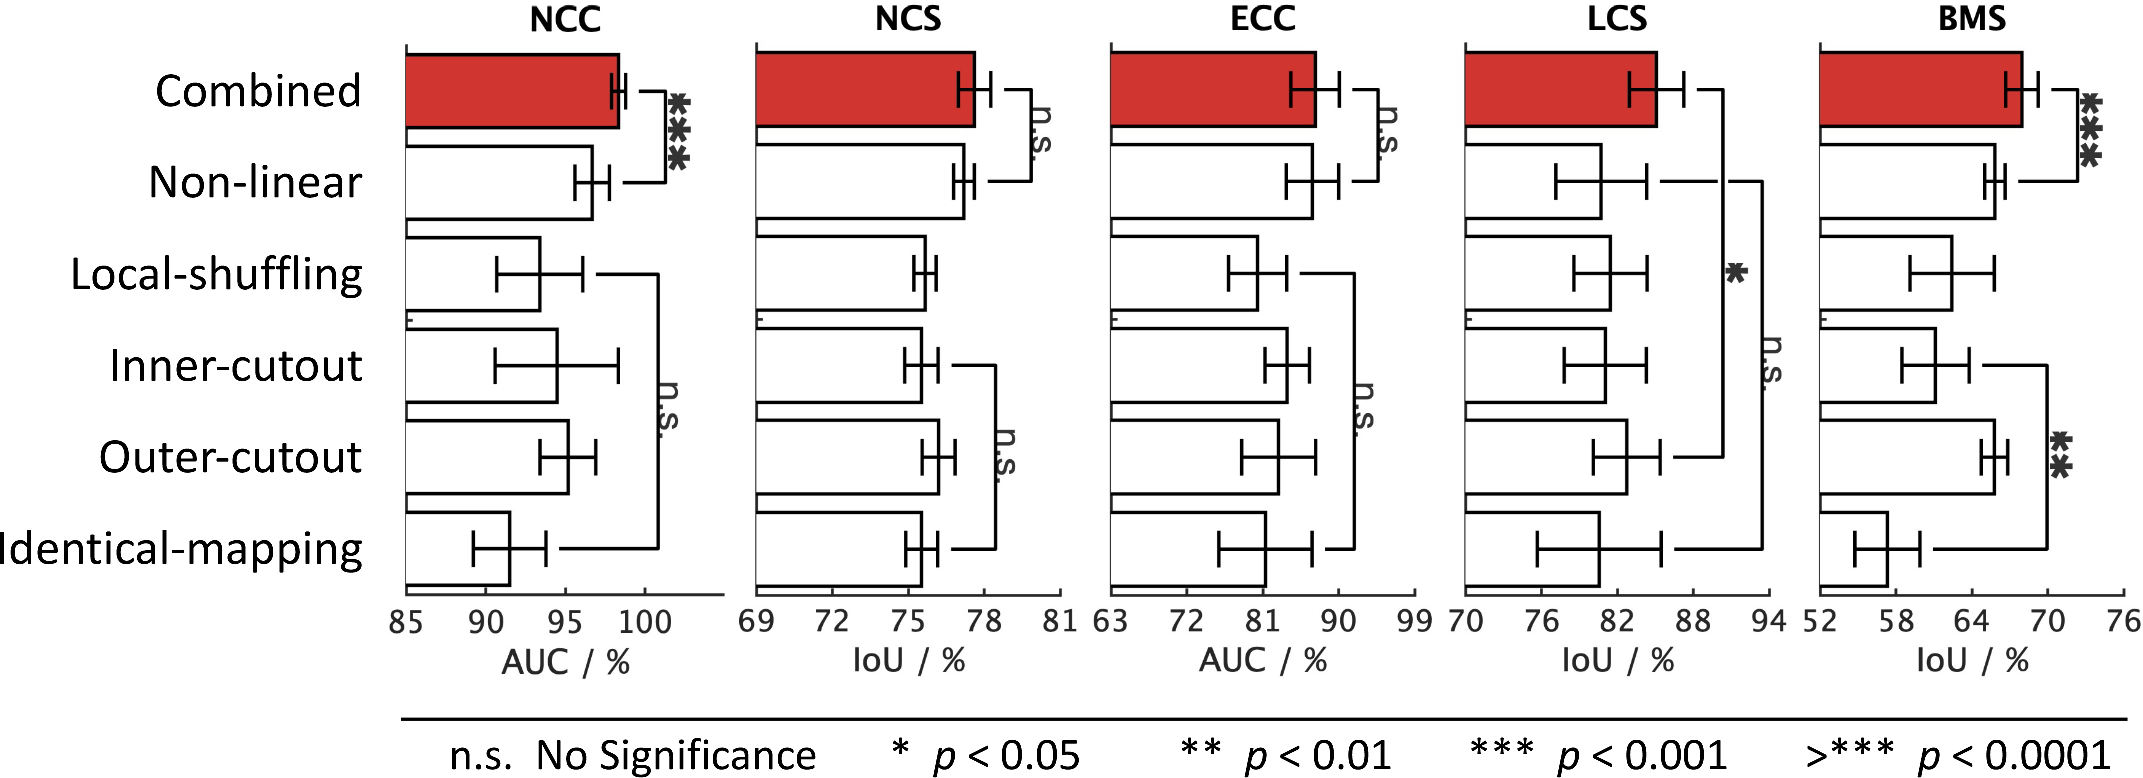
\includegraphics[width=0.9\columnwidth]{Figures/CH5/fig_combined_vs_individuals.pdf}
\end{center}
\caption[The Combined Learning Scheme Exceeds Each Individual]{
Comparing the combined training scheme with each of the proposed individual training schemes, we conduct statistical analyses between the top two training schemes as well as between the bottom two. Although some of the individual training schemes could be favorable for certain target tasks, there is no such clear clue to guarantee that any one of the individual training schemes would consistently offer the best performance on every target task. On the contrary, our combined training scheme consistently achieves the best results across all five target tasks.
}
\label{ch5:fig:combined_vs_individuals}
\end{sidewaysfigure}

% \fillandplacepagenumber
% \end{landscape}
%%%%%%%%%%%%%%%%%%%%%%%%%%%%%%%%%%%%%%%%%%%%

\subsection{The Combined Learning Scheme Exceeds Each Individual}
\label{ch5:individual_combination}


We have devised four individual training schemes by applying each of the transformations (\ie non-linear, local-shuffling, outer-cutout, and inner-cutout) individually to a sub-volume and training the model to restore the original one. We compare each of these training schemes with identical-mapping, which does not involve any image transformation\footnote{I acknowledge Vatsal Sodha, with whom I co-authored~\citet{zhou2019models,zhou2021models}, for comparing the combined learning scheme with each individual.}. In three out of the five target tasks, as shown in Figs.~\ref{ch5:fig:combined_vs_individuals}---\ref{ch5:fig:random_initialization}, the model pre-trained by identical-mapping scheme does not perform as well as random initialization. This undesired representation obtained via identical-mapping suggests that without any image transformation, the model would not benefit much from the proxy image restoration task. On the contrary, nearly all of the individual schemes offer higher target task performances than identical-mapping, demonstrating the significance of the four devised image transformations in learning image representation. 

Although each of the individual schemes has established the capability in learning image representation, its empirical performance varies from task to task. That being said, given a target task, there is no clear winner among the four individual schemes that can always guarantee the highest performance. As a result, we have further devised a combined scheme, which applies transformations to a sub-volume with a predefined probability for each transformation and trains a model to restore the original one. To demonstrate the importance of combining these image transformations together, we examine the combined training scheme against each of the individual ones. \figurename~\ref{ch5:fig:combined_vs_individuals} shows that the combined scheme consistently exceeds any other individual schemes in all five target tasks. We have found that the combination of different transformations is advantageous because, as discussed, we cannot rely on one single training scheme to achieve the most robust and compelling results across multiple target tasks. 
It is our novel representation learning framework based on image restoration that allows integrating various training schemes into a single training scheme. Our qualitative assessment of image restoration quality further indicates that the combined scheme is superior over all four individual schemes in restoring the images that have been undergone multiple transformations. In summary, our combined scheme pre-trains a model from multiple perspectives (appearance, texture, context, etc.), empowering models to learn a more comprehensive representation, thereby leading to more robust target models. Based on the above ablation studies, in the following sections, we refer the models pre-trained by the combined scheme to Models Genesis and, in particular, refer the model pre-trained on LUNA~2016 dataset to Genesis Chest CT.


%%%%%%%%%%%%%%%%%%%%%%%%%%%%%%%%%%%%%%%%%%%%
% \begin{landscape}
% \thispagestyle{empty}

\begin{sidewaysfigure}
\begin{center}
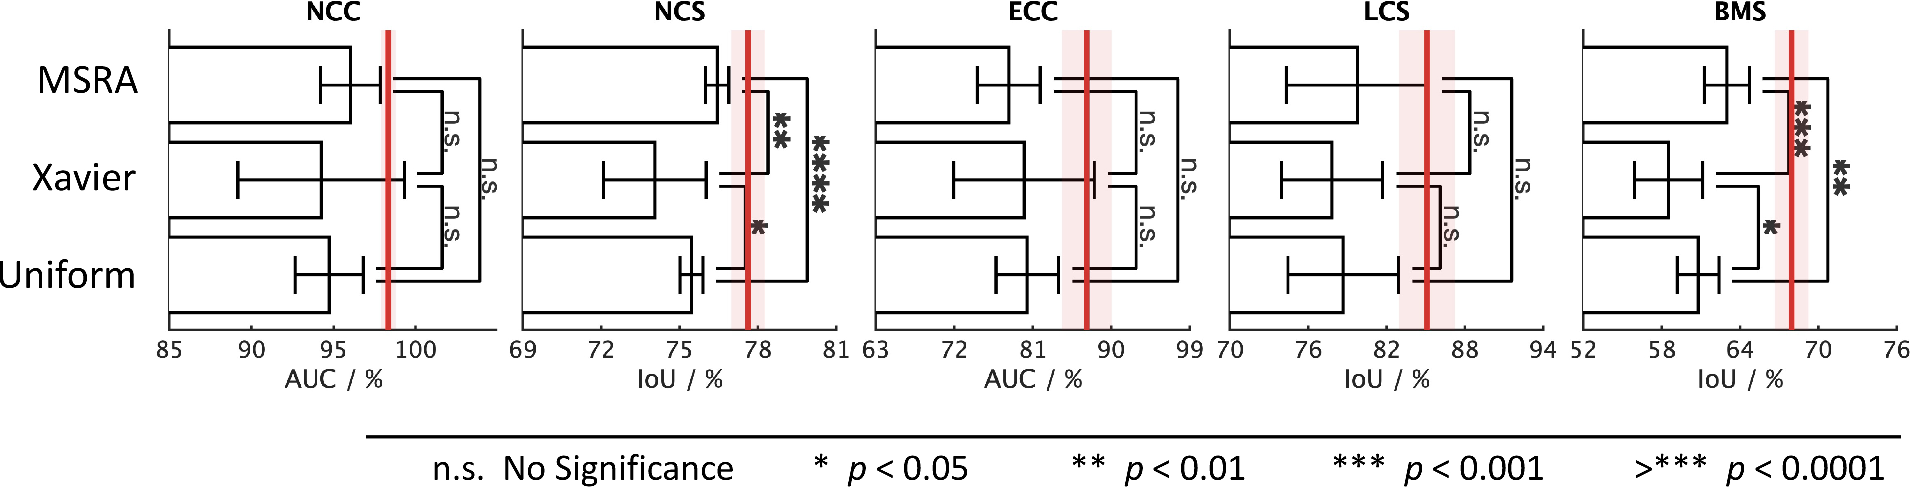
\includegraphics[width=0.9\columnwidth]{Figures/CH5/fig_among_scratch.pdf}
\end{center}
\caption[Models Genesis Outperform Learning from Scratch]{
Models Genesis, as presented with the red vertical lines, achieve higher and more stable performance compared with three popular types of random initialization methods, including MSRA, Xavier, and Uniform. Among three out of the five applications, three different types of random distribution reveal no significant difference with respect to each other.
}
\label{ch5:fig:random_initialization}
\end{sidewaysfigure}

% \fillandplacepagenumber
% \end{landscape}
%%%%%%%%%%%%%%%%%%%%%%%%%%%%%%%%%%%%%%%%%%%%

%%%%%%%%%%%%%%%%%%%%%%%%%%%%%%%%%%%%%%%%%%%%
% \begin{landscape}
% \thispagestyle{empty}

\begin{sidewaysfigure}
\begin{center}
\includegraphics[width=1.0\columnwidth]{Figures/CH5/fig_learning_curve.pdf}
\end{center}
\caption[Models Genesis Enable Better Optimization than Learning from Scratch]{
Models Genesis enable better optimization than learning from scratch, evident by the learning curves for the target tasks of reducing false positives in detecting lung nodules (\texttt{NCC}) and pulmonary embolism (\texttt{ECC}) as well as segmenting lung nodule (\texttt{NCS}), liver (\texttt{LCS}), and brain tumor (\texttt{BMS}). We have plotted the validation performance averaged by ten trials for each application, in which accuracy and dice-coefficient scores are reported for classification and segmentation tasks, respectively. As seen, initializing with our pre-trained Models Genesis demonstrates benefits in the convergence speed.
}
\label{ch5:fig:learning_curve}
\end{sidewaysfigure}

% \fillandplacepagenumber
% \end{landscape}
%%%%%%%%%%%%%%%%%%%%%%%%%%%%%%%%%%%%%%%%%%%%

\subsection{Models Genesis Outperform Learning from Scratch}
\label{ch5:surpass_scratch}


Transfer learning accelerates training and boosts performance, only if the image representation learned from the original (proxy) task is general and transferable to target tasks. Fine-tuning models trained on ImageNet has been a great success story in 2D~\citep{bar2015chest,tajbakhsh2016convolutional,shin2016deep}, but for 3D representation learning, there is no such a massive labeled dataset like ImageNet. As a result, it is still common practice to train 3D model from scratch in 3D medical imaging.
Therefore, to establish the 3D baselines, we have trained 3D models with three representative random initialization methods\footnote{I thank Pengfei Zhang for comparing Xavier/Glorot and He normal (MSRA) initialization methods with our Models Genesis.}, including naive uniform initialization, Xavier/Glorot initialization proposed by~\citet{glorot2010understanding}, and He normal (MSRA) initialization proposed by~\citet{he2015delving}. 
When comparing deep model initialization by transfer learning and by controlling mathematical distribution, the former learns more sophisticated image representation but suffers from a domain gap, whereas the latter is task independent yet provides relatively less benefit than the former. The hypothesis underneath transfer learning is that transferring deep features across visual tasks can obtain a semantically more powerful representation, compared with simply initializing weights using different distributions.
From our comprehensive experiments in~\figurename~\ref{ch5:fig:random_initialization}, we have observed the following:
\begin{itemize}
    \item Within each method, random initialization of weights has shown large variance in results of ten trials; it is in large part due to the difficulty of adequately initializing these networks from scratch. A small miscalibration of the initial weights can lead to vanishing or exploding gradients, as well as poor convergence properties. 
    \item In three out of the five 3D medical applications, the results reveal no significant difference among these random initialization methods. Although randomly initializing weights can vary by the behaviors on different applications, He normal (MSRA), in which the weights are initialized with a specific ReLU-aware initialization, generally works the most reliably among all five target tasks.
    \item On the other hand, initialization with our pre-trained Genesis Chest CT stabilizes the overall performance and, more importantly, elevates the average performance over all three random initialization methods by a large margin. Our statistical analysis shows that the performance gain is significant for all the target tasks under study. This suggests that, owing to the representation learning scheme, our initial weights provide a better starting point than the ones generated under particular statistical distributions, while being over 13\% faster (see \figurename~\ref{ch5:fig:learning_curve}). This observation has also been widely obtained in 2D model initialization~\citep{tajbakhsh2016convolutional,shin2016deep,rawat2017deep,zhou2017fine,voulodimos2018deep}.
\end{itemize}

Altogether, in contrast to 3D scratch models, we believe Models Genesis can potentially serve as a primary source of transfer learning for 3D medical imaging applications. Besides contrasting with the three random initialization methods, we further examine our Models Genesis against the existing pre-trained 3D models in the coming section.



%%%%%%%%%%%%%%%%%%%%%%%%%%%%%%%%%%%%%%%%%%%%
% \begin{landscape}
% \thispagestyle{empty}

\begin{sidewaystable}
\begin{threeparttable}[t]
\begin{center}
\footnotesize
\caption[Models Genesis Surpass Existing Pre-trained 3D Models]{
Models Genesis surpass existing pre-trained 3D models. We evaluate AUC score for classification tasks and IoU score for segmentation tasks. All of the results, including the mean and standard deviation (mean$\pm$s.d.) across ten trials. For every target task, we have further performed independent two sample $t$-test between the best (bolded) vs. others and highlighted boxes in blue when they are not statistically significantly different at $p=0.05$ level.
% Our Models Genesis lead the best or comparable performance on five distinct medical target tasks over six self-supervised learning approaches (revised in 3D) and three competing publicly available (fully) supervised pre-trained 3D models. For ease of comparison, we evaluate AUC score for the two classification tasks (\ie \texttt{NCC} and \texttt{ECC}) and IoU score for the three segmentation tasks (\ie \texttt{NCS}, \texttt{LCS}, and \texttt{BMS}). All of the results, including the mean and standard deviation (mean$\pm$s.d.) across ten trials, reported in the table are evaluated using our dataset splitting, elaborated in~Appendix~\ref{ap1}. For every target task, we have further performed independent two sample $t$-test between the best (bolded) vs. others and highlighted boxes in blue when they are not statistically significantly different at $p=0.05$ level.
}
\label{ch5:tab:top_existing_models}
\begin{tabular}{p{0.14\linewidth}p{0.2\linewidth}P{0.1\linewidth}P{0.1\linewidth}P{0.1\linewidth}P{0.1\linewidth}P{0.1\linewidth}}
    \hline
    \multirow{2}{*}{Pre-training} & \multirow{2}{*}{Approach} & \multicolumn{5}{c}{Target tasks} \\
    \cline{3-7}
     & & \texttt{NCC} (\%) & \texttt{NCS} (\%) & \texttt{ECC} (\%) & \texttt{LCS} (\%) & \texttt{BMS} (\%) \\
    \hline
    \multirow{3}{*}{No} & Random with Uniform Init & 94.74$\pm$1.97 & 75.48$\pm$0.43 & 80.36$\pm$3.58 & 78.68$\pm$4.23 & 60.79$\pm$1.60 \\
     & Random with Xavier Init & 94.25$\pm$5.07 & 74.05$\pm$1.97 & 79.99$\pm$8.06 & 77.82$\pm$3.87 & 58.52$\pm$2.61 \\
     & Random with MSRA Init & 96.03$\pm$1.82 & 76.44$\pm$0.45 & 78.24$\pm$3.60 & 79.76$\pm$5.43 & 63.00$\pm$1.73 \\
    \hline
    \multirow{3}{*}{(Fully) supervised} & I3D & \cellcolor{iblue!30}98.26$\pm$0.27 & 71.58$\pm$0.55 & 80.55$\pm$1.11 & 70.65$\pm$4.26 & \cellcolor{iblue!30}67.83$\pm$0.75 \\
     & NiftyNet & 94.14$\pm$4.57 & 52.98$\pm$2.05 & 77.33$\pm$8.05 & 83.23$\pm$1.05 & 60.78$\pm$1.60  \\
     & MedicalNet & 95.80$\pm$0.49 & 75.68$\pm$0.32 & \cellcolor{iblue!30}86.43$\pm$1.44 & \cellcolor{iblue!30}\textbf{85.52$\pm$0.58} & 66.09$\pm$1.35 \\
    \hline
    \multirow{7}{*}{Self-supervised} & De-noising & 95.92$\pm$1.83 & 73.99$\pm$0.62 & \cellcolor{iblue!30}85.14$\pm$3.02 & 84.36$\pm$0.96 & 57.83$\pm$1.57 \\
     & In-painting & 91.46$\pm$2.97 & 76.02$\pm$0.55 & 79.79$\pm$3.55 & 81.36$\pm$4.83 & 61.38$\pm$3.84 \\
     & Jigsaw & 95.47$\pm$1.24 & 70.90$\pm$1.55 & 81.79$\pm$1.04 & 82.04$\pm$1.26 & 63.33$\pm$1.11 \\
     & DeepCluster & 97.22$\pm$0.55 & 74.95$\pm$0.46 & 84.82$\pm$0.62 & 82.66$\pm$1.00 & 65.96$\pm$0.85 \\
     & Patch shuffling & 91.93$\pm$2.32 & 75.74$\pm$0.51 & 82.15$\pm$3.30 & 82.82$\pm$2.35 & 52.95$\pm$6.92 \\
     & Rubik’s Cube & 96.24$\pm$1.27 & 72.87$\pm$0.16 & 80.49$\pm$4.64 & 75.59$\pm$0.20 & 62.75$\pm$1.93 \\
     & Genesis Chest CT (ours) & \cellcolor{iblue!30}\textbf{98.34$\pm$0.44} & \cellcolor{iblue!30}\textbf{77.62$\pm$0.64} & \cellcolor{iblue!30}\textbf{87.20$\pm$2.87} & \cellcolor{iblue!30}85.10$\pm$2.15 & \cellcolor{iblue!30}\textbf{67.96$\pm$1.29} \\
    \hline
    \end{tabular}
    \begin{tablenotes}
        \item 
    \end{tablenotes}
\end{center}
\end{threeparttable}
\end{sidewaystable}
% \fillandplacepagenumber
% \end{landscape}
%%%%%%%%%%%%%%%%%%%%%%%%%%%%%%%%%%%%%%%%%%%%



\subsection{Models Genesis Surpass Existing Pre-trained 3D Models}
\label{ch5:public_3d_model}

We have evaluated our Models Genesis with existing publicly available pre-trained 3D models on five distinct medical target tasks\footnote{I thank Zuwei Guo for implementing Rubik's Cube~\citep{zhuang2019self} and the 3D version of Jigsaw~\citep{noroozi2016unsupervised} and DeepCluster~\citep{caron2018deep}; Jiaxuan Pang for comparing I3D~\citep{carreira2017quo} with our Models Genesis; Fatemeh Haghighi and Mohammad Reza Hosseinzadeh Taher for implementing the 3D version of in-painting~\citep{pathak2016context}, patch-shuffling~\citep{chen2019self}, and working with Zuwei Guo in evaluating the performance of MedicalNet~\citep{chen2019med3d}; Md Mahfuzur Rahman Siddiquee for examining NiftyNet~\citep{gibson2018niftynet} with our Models Genesis.}. As shown in \tablename~\ref{ch5:tab:top_existing_models}, Genesis Chest CT noticeably contrasts with any other existing 3D models, which have been pre-trained by full supervision. Note that, in the liver segmentation task (\texttt{LCS}), Genesis Chest CT is slightly outperformed by MedicalNet because of the benefit that MedicalNet gained from its (fully) supervised pre-training  on the LiTS dataset directly. Further statistical tests reveal that Genesis Chest CT still yields comparable performance with MedicalNet at $p=0.05$ level. For the rest four target tasks, Genesis Chest CT achieves superior performance against all its counterparts by a large margin, demonstrating the effectiveness and transferability of the learned features of Models Genesis, which are beneficial for both classification and segmentation tasks. 

More importantly, although Genesis Chest CT is pre-trained on Chest CT only, it can generalize to different organs, diseases, datasets, and even modalities. For instance, the target task of pulmonary embolism false positive reduction is performed in Contrast-Enhanced CT scans that can appear differently from the proxy tasks in normal CT scans; yet, Genesis Chest CT achieves a remarkable improvement over training from scratch, increasing the AUC by 7 points. Moreover, Genesis Chest CT continues to yield a significant IoU gain in liver segmentation even though the proxy task and target task are significantly different in both, diseases affecting the organs (lung vs.~liver) and the dataset itself (LUNA~2016 vs.~LiTS~2017). We have further examined Genesis Chest CT and other existing pre-trained models using MRI Flair images, which represent the widest domain distance between the proxy and target tasks. As reported in \tablename~\ref{ch5:tab:top_existing_models} (\texttt{BMS}), Genesis Chest CT yields nearly a 5-point improvement in comparison with random initialization. The increased performance on the MRI imaging task is a particularly strong demonstration of the transfer learning capabilities of our Genesis Chest CT. 
% To further investigate the behavior of Genesis Chest CT when encountering medical images from different modalities, we have provided extensive visualization in \figurename~\ref{ch5:fig:xray_across_restoration}, including example images from CT, X-ray, Ultrasound, and MRI modalities.

Considering the model footprint, our Models Genesis take the basic 3D U-Net as the backbone, carrying much fewer parameters than the existing open-source pre-trained 3D models. For example, we have adopted MedicalNet with resnet-101 as the backbone, which offers the highest performance based on \citet{chen2019med3d} but comprises of 85.75M parameters; the pre-trained I3D~\citep{carreira2017quo} contains 25.35M parameters in the encoder; \iffalse and 134.65M when adding a decoder for segmentation;\fi the pre-trained NiftyNet uses Dense V-Networks~\citep{gibson2018automatic} as backbone, comprising of only 2.60M parameters, but it does not perform as well as its counterparts in all five target tasks. Taken together, these results indicate that our Models Genesis, with only 16.32M parameters, surpass all existing pre-trained 3D models in terms of generalizability, transferability, and parameter efficiency.


%%%%%%%%%%%%%%%%%%%%%%%%%%%%%%%%%%%%%%%%%%%%
% \begin{landscape}
% \thispagestyle{empty}

\begin{sidewaysfigure}
\begin{center}
\includegraphics[width=1.0\columnwidth]{Figures/CH5/fig_annotation_cost.pdf}
\caption[Models Genesis Reduce Annotation Efforts by at Least 30\%]{
Initializing with our Models Genesis, the annotation cost can be reduced by 30\%, 50\%, 57\%, 84\%, and 44\% for target tasks \texttt{NCC}, \texttt{NCS}, \texttt{ECC}, \texttt{LCS}, and \texttt{BMS}, respectively. With decreasing amounts of labeled data, Models Genesis (red) retain a much higher performance on all five target tasks, whereas learning from scratch (grey) fails to generalize. Note that the horizontal red and gray lines refer to the performances that can eventually be achieved by Models Genesis and learning from scratch, respectively, when using the entire dataset.
}
\label{ch5:fig:annotation_cost}
\end{center}
\end{sidewaysfigure}

% \fillandplacepagenumber
% \end{landscape}
%%%%%%%%%%%%%%%%%%%%%%%%%%%%%%%%%%%%%%%%%%%%


\subsection{Models Genesis Reduce Annotation Efforts by at Least 30\%}
\label{ch5:annotation_effort}

While critics often stress the need for sufficiently large amounts of labeled data to train a deep model, transfer learning leverages the knowledge about medical images already learned by pre-trained models and therefore requires considerably fewer annotated data and training iterations than learning from scratch. We have simulated the scenarios of using a handful of labeled data, which allows investigating the power of our Models Genesis in transfer learning. \figurename~\ref{ch5:fig:annotation_cost} displays the results of training with a partial dataset, demonstrating that fine-tuning Models Genesis saturates quickly on the target tasks since it can achieve similar performance compared with the full dataset training. 
Specifically, the performance of learning 3D models from scratch with entire datasets can be approximated using Models Genesis with only 50\%, 5\%, 30\%, 5\%, and 30\% of datasets for \texttt{NCC}, \texttt{NCS}, \texttt{ECC}, \texttt{LCS}, and \texttt{BMS}, respectively. 
This shows that our Models Genesis can mitigate the lack of labeled images, resulting in a more annotation efficient deep learning in the end. 

Furthermore, the performance gap between fine-tuning and learning from scratch is significant and steady over training models with each partial data point. For the lung nodule false positive reduction target task (\texttt{NCC} in~\figurename~\ref{ch5:fig:annotation_cost}), using only 49\% training data, Models Genesis equal the performance of 70\% training data learning from scratch. Therefore, about 30\% of the annotation cost associated with learning from scratch in \texttt{NCC} is recovered by initializing with Models Genesis. For the lung nodule segmentation target task (\texttt{NCS} in~\figurename~\ref{ch5:fig:annotation_cost}), with 5\% training data, Models Genesis can achieve the performance equivalent to learning from scratch using 10\% training data. Based on this analysis, the cost of annotation in \texttt{NCS} can be reduced by half using Models Genesis compared with learning from scratch. For the pulmonary embolism false positive reduction target task (\texttt{ECC}),~\figurename~\ref{ch5:fig:annotation_cost} suggests that with only 30\% training samples, Models Genesis achieve performance equivalent to learning from scratch using 70\% training samples. Therefore, nearly 57\% of the labeling cost associated with the use of learning from scratch for \texttt{ECC} could be recovered with our Models Genesis. For the liver segmentation target task (\texttt{LCS}) in~\figurename~\ref{ch5:fig:annotation_cost}, using 8\% training data, Models Genesis equal the performance of learning from scratch using 50\% training samples. Therefore, about 84\% of the annotation cost associated with learning from scratch in \texttt{LCS} is recovered by initializing with Models Genesis. For the brain tumor segmentation target task (\texttt{BMS}) in~\figurename~\ref{ch5:fig:annotation_cost}, with less than 28\% training data, Models Genesis achieve the performance equivalent to learning from scratch using 50\% training data. Therefore, nearly 44\% annotation efforts can be reduced using Models Genesis compared with learning from scratch. Overall, at least 30\% annotation efforts have been reduced by Models Genesis, in comparison with learning a 3D model from scratch in five target tasks. With such annotation-efficient 3D transfer learning paradigm, computer-aided diagnosis of rare diseases or rapid response to global pandemics, which are severely underrepresented owing to the difficulty of collecting a sizeable amount labeled data, could be eventually actualized.

%%%%%%%%%%%%%%%%%%%%%%%%%%%%%%%%%%%%%%%%%%%%
% \begin{landscape}
% \thispagestyle{empty}

\begin{sidewaysfigure}
\centering
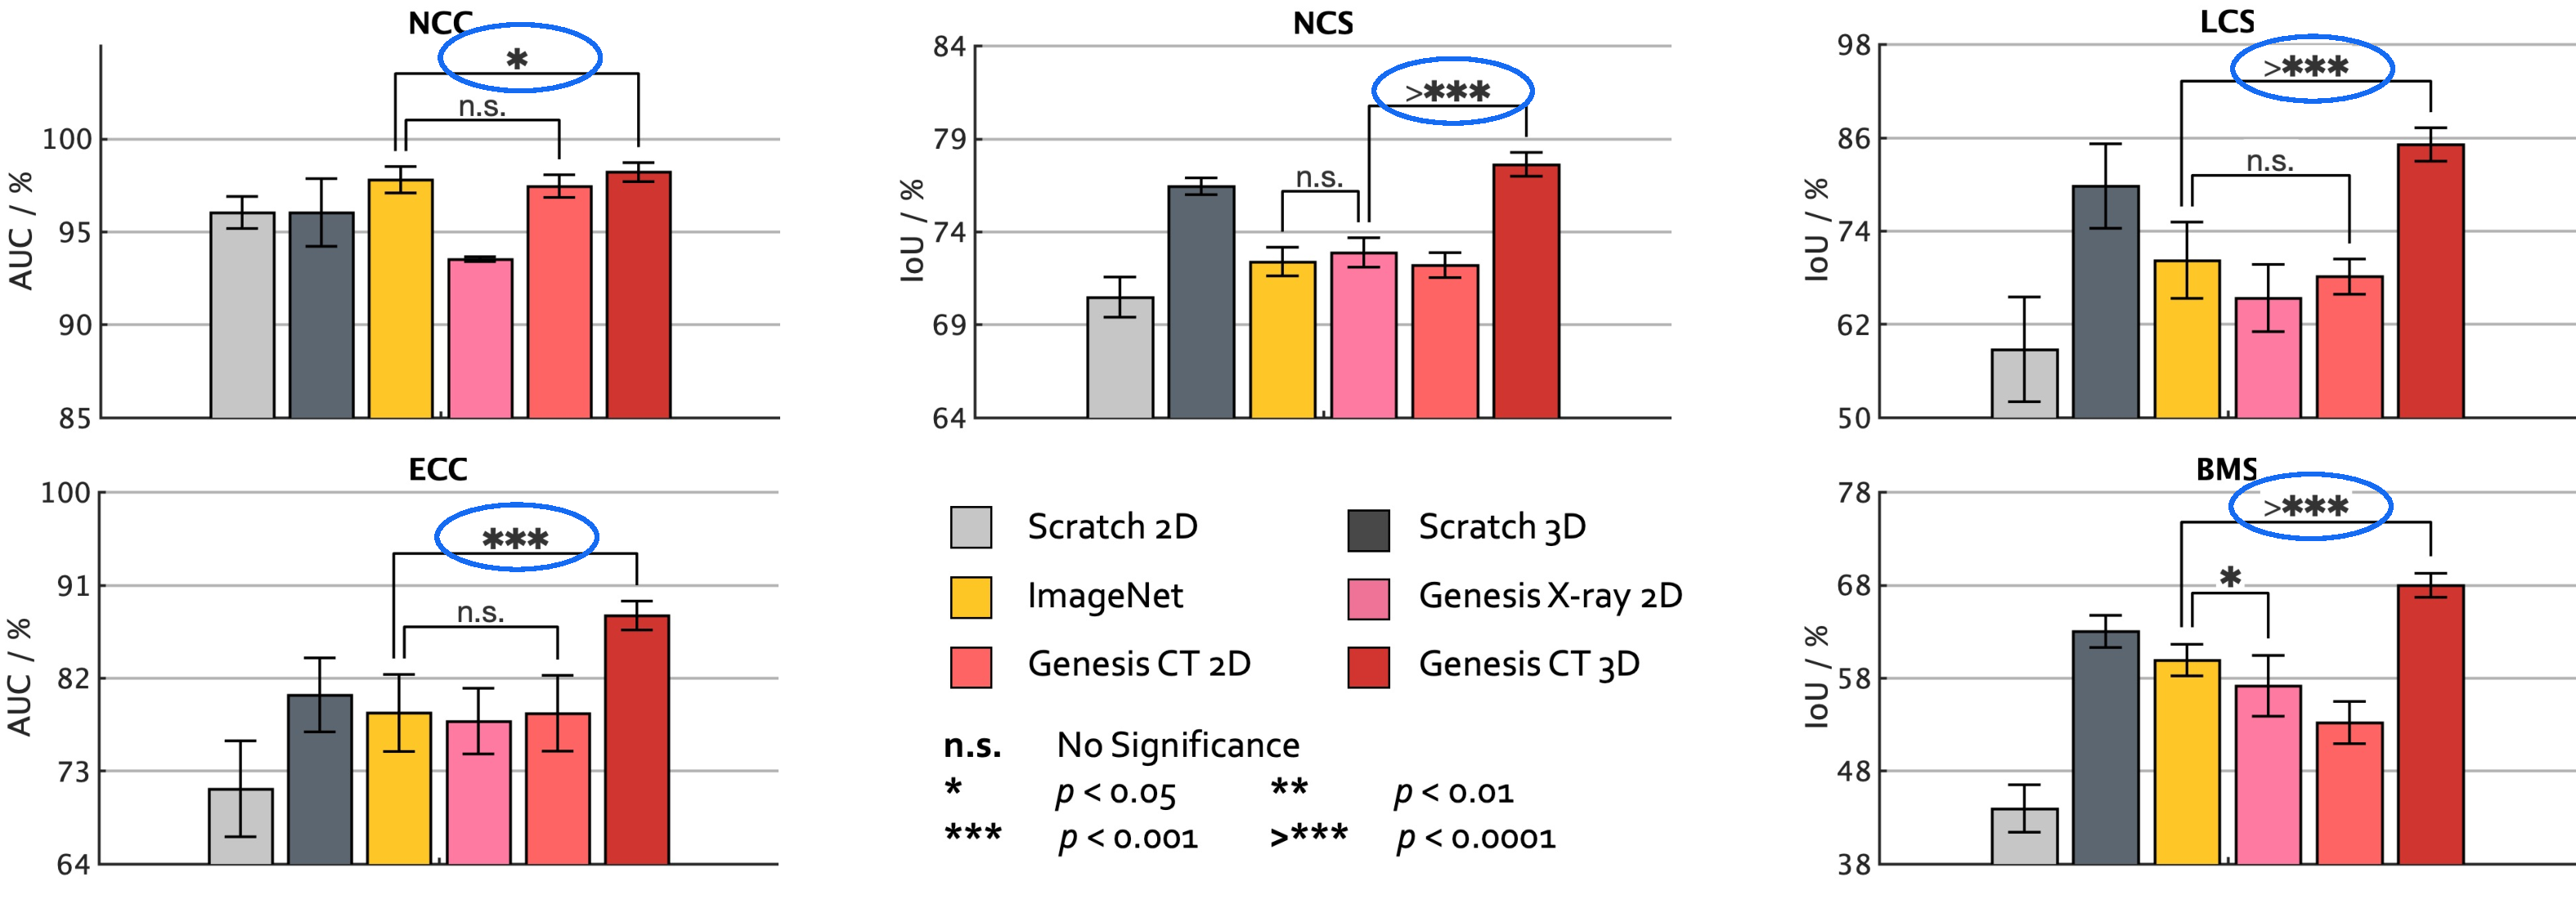
\includegraphics[width=1.0\columnwidth]{Figures/CH5/fig_3d_vs_2d.pdf}
\caption[Models Genesis Top Any 2D Approaches]{
When solving problems in volumetric medical modalities, such as CT and MRI images, 3D \textit{volume-based} approaches consistently offer superior performance than 2D \textit{slice-based} approaches empowered by transfer learning. We conduct statistical analyses (circled in blue) between the highest performance achieved by 3D and 2D solutions. Training 3D models from scratch does not necessarily outperform their 2D counterparts (see \texttt{NCC}). However, training the same 3D models from Genesis Chest CT outperforms all their 2D counterparts, including fine-tuning Models ImageNet as well as fine-tuning our Genesis Chest X-ray and Genesis Chest CT 2D. It confirms the effectiveness of Genesis Chest CT in unlocking the power of 3D models. In addition, we have also provided statistical analyses between the highest and the second highest performances achieved by 2D models, finding that Models Genesis (2D) offer equivalent performances (n.s.) to Models ImageNet in four out of the five applications.
}
\label{ch5:fig:2D_3D_target_tasks}
\end{sidewaysfigure}

% \fillandplacepagenumber
% \end{landscape}
%%%%%%%%%%%%%%%%%%%%%%%%%%%%%%%%%%%%%%%%%%%%


\begin{table}[t]
\centering
\footnotesize
\caption[Models Genesis Top Any 2D/2.5D Approaches]{
Our 3D approach, initialized by Models Genesis, significantly elevates the classification performance compared with 2.5D and 2D approaches in reducing lung nodule and pulmonary embolism false positives. The entries in bold highlight the best results achieved by different approaches. For the 2D slice-based approach, we extract input consisting of three adjacent axial views of the lung nodule or pulmonary embolism and some of their surroundings. For the 2.5D orthogonal approach, each input is composed of an axial, coronal, and sagittal slice and centered at a lung nodule or pulmonary embolism candidate.
}
\label{ch5:tab:3d_2.5d_2d}
\begin{tabular}{p{0.35\linewidth}P{0.18\linewidth}P{0.18\linewidth}P{0.18\linewidth}}
    \hline
    Task: \texttt{NCC} & Random & ImageNet & Genesis \\
    \hline
    2D slice-based input & 96.03$\pm$0.86 & \textbf{97.79$\pm$0.71} & 97.45$\pm$0.61 \\
    2.5D orthogonal input & 95.76$\pm$1.05 & \textbf{97.24$\pm$1.01} & 97.07$\pm$0.92 \\
    3D volume-based input & 96.03$\pm$1.82 & n/a & \textbf{98.34$\pm$0.44} \\
    \hline
    \hline
    Task: \texttt{ECC} & Random & ImageNet & Genesis \\
    \hline
    2D slice-based input & 60.33$\pm$8.61 & 62.57$\pm$8.04 & \textbf{62.84$\pm$8.78} \\
    2.5D orthogonal input & 71.27$\pm$4.64 & \textbf{78.61$\pm$3.73} & 78.58$\pm$3.67 \\
    3D volume-based input & 80.36$\pm$3.58 & n/a & \textbf{88.04$\pm$1.40} \\
    \hline
    \end{tabular}
\end{table}

\subsection{Models Genesis Top Any 2D/2.5D Approaches}
\label{ch5:models_genesis_top_2D}

We have thus far presented the power of 3D models in processing volumetric data, in particular, with limited annotation. Besides adopting 3D models, another common strategy to handle limited data in volumetric medical imaging is to reformat 3D data into a 2D image representation followed by fine-tuning pre-trained Models ImageNet~\citep{shin2016deep,tajbakhsh2016convolutional}. This approach increases the training examples by order of magnitude, but it sacrifices the 3D context. It is interesting to note how Genesis Chest CT compares with this \textit{de facto} standard in 2D. We have thus implemented two different methods to reformat 3D data into 2D input\footnote{I thank Jae Y. Shin for organizing and pre-processing the PE dataset.}: the regular 2D representation obtained by extracting adjacent axial slices~\citep{ben2016fully,sun2017multiphase}, and the 2.5D representation~\citep{prasoon2013deep,roth2014new,roth2015improving} composed of axial, coronal, and sagittal slices from volumetric data. Both of these 2D approaches seek to use 2D representation to emulate something three dimensional, in order to fit the paradigm of fine-tuning Models ImageNet. 
In the inference, classification and segmentation tasks are evaluated differently in 2D: for classification, the model predicts labels of slices extracted from the center locations because other slices are not guaranteed to include objects; for segmentation, the model predicts segmentation mask slice by slice and form the 3D segmentation volume by simply stacking the 2D segmentation maps.


\figurename~\ref{ch5:fig:2D_3D_target_tasks} exposes the comparison between 3D and 2D models on five 3D target tasks. Additionally, \tablename~\ref{ch5:tab:3d_2.5d_2d} compares 2D slice-based, 2.5D orthogonal, and 3D volume-based approaches on lung nodule and pulmonary embolism false positive reduction tasks. As evidenced by our statistical analyses, the 3D models trained from Genesis Chest CT achieve significantly higher average performance and lower standard deviation than 2D models fine-tuned from ImageNet using either 2D or 2.5D image representation. Nonetheless, the same conclusion does not apply to the models trained from scratch---3D scratch models are outperformed by 2D models in one out of the five target tasks (\ie \texttt{NCC} in \figurename~\ref{ch5:fig:2D_3D_target_tasks} and \tablename~\ref{ch5:tab:3d_2.5d_2d}) and also exhibit an undesirably larger standard deviation. We attribute the mixed results of 3D scratch models to the larger number of model parameters and limited sample size in the target tasks, which together impede the full utilization of 3D context. In fact, the undesirable performance of the 3D scratch models highlights the effectiveness of Genesis Chest CT, which unlocks the power of 3D models for medical imaging. To summarize, we believe that 3D problems in medical imaging should be solved in 3D directly.


\section{Discussion \& Conclusion}
\label{ch5:discussion}

%%moved to here
\subsection{Do We Still Need a Medical ImageNet?}
\label{ch5:medical_imagenet}

In computer vision, at the time this chapter is written, no self-supervised learning method outperforms fine-tuning models pre-trained on ImageNet~\citep{jing2020self,chen2019self,kolesnikov2019revisiting,zhou2019models,hendrycks2019using,zhang2019aet,caron2019unsupervised}. Therefore, it may seem surprising to observe from our results in \tablename~\ref{ch5:tab:top_existing_models} that (fully) supervised representation learning methods do not necessarily offer higher performances in some 3D target tasks than self-supervised representation learning methods. We ascribe this phenomenon to the limited amount of supervision used in their pre-training (90 cases for NiftyNet~\citep{gibson2018niftynet} and 1,638 cases for MedicalNet~\citep{chen2019med3d}) or the domain distance (from videos to CT/MRI for I3D~\citep{carreira2017quo}). Evidenced by a prior study~\citep{sun2017revisiting} on ImageNet pre-training, large amount of supervision is required to foster a generic, comprehensive image representation. Back in 2009, when ImageNet had not been established, it was challenging to empower a deep model with generic image representation using a small or even medium size of labeled data, the same situation, we believe, that presents in 3D medical image analysis today. Therefore, despite the outstanding performance of Models Genesis, there is no doubt that a large, strongly annotated dataset for medical image analysis, like ImageNet~\citep{deng2009imagenet} for computer vision, is still highly demanded. One of our goals for developing Models Genesis is to help create such a medical ImageNet. Based on a small set of expert annotations, models fine-tuned from Models Genesis will be able to help quickly generate initial rough annotations of unlabeled images for expert review, thus reducing the annotation efforts and accelerating the creation of a large, strongly annotated, medical ImageNet. In summary, Models Genesis are not designed to replace such a large, strongly annotated dataset for medical image analysis, as ImageNet for computer vision, but rather to help create one.



\subsection{Same-domain or Cross-domain Transfer Learning?}
\label{ch5:same_cross_modality}

Same-domain transfer learning is always preferred whenever possible because a relatively smaller domain gap makes the learned image representation more beneficial for target tasks. Even the most recent self-supervised learning approaches in medical imaging were solely evaluated within the same dataset, such as~\citet{chen2019self,tajbakhsh2019surrogate,zhu2020rubik}. Same-domain transfer learning strikes as a preferred choice in terms of performance; however, most of the existing medical datasets, with less than hundred cases, are usually too small for deep models to learn reliable image representation. Therefore, for our future work, we plan to combine the publicly available datasets from similar domains together to train modality-oriented models, including Genesis CT, Genesis MRI, Genesis X-ray, and Genesis Ultrasound, as well as organ-oriented models, including Genesis Brain, Genesis Lung, Genesis Heart, and Genesis Liver. 

Cross-domain transfer learning in medical imaging is the Holy Grail. Retrieving a large number of unlabeled images from a PACS system requires an IRB approval, often a long process; the retrieved images must be de-identified; organizing the de-identified images in a way suitable for deep learning is tedious and laborious. Therefore, large quantities of unlabeled datasets may not be readily available to many target domains. Evidenced by our results in \tablename~\ref{ch5:tab:top_existing_models} (\texttt{BMS}), Models Genesis have a great potential for cross-domain transfer learning; particularly, our distortion-based approaches (such as non-linear and local-shuffling) take advantage of relative intensity values (in all modalities) to learn shapes and appearances of various organs. Therefore, as our future work, we will be focusing on methods that generalize well across domains. 


\subsection{Is Any Data Augmentation Suitable as a Transformation?} 
\label{ch5:choice_transformations}

We propose a self-supervised learning framework to learn image representation by discriminating and restoring images undergoing different transformations. One might argue that our image transformations can be interchangeable with existing data augmentation techniques~\citep{gan2015learning,wong2016understanding,perez2017effectiveness,shorten2019survey}, while we would like to make the distinction between these two concepts clearer. It is critical to assess whether a specific augmentation is practical and feasible for the image restoration task when designing image transformations. Simply introducing data augmentation can make a task ambiguous and lead to degenerate learning. To this end, we choose image transformations based on two principles:
\begin{itemize}
    \item First, the transformed sub-volume should not be found in the original CT scan. But it is possible to find a transformed sub-volume that has undergone such augmentations as rotation, flip, zoom in/out, or translation, as an alternative sub-volume in the original CT scan. In this scenario, without additional spatial information, the model would not be able to ``recover'' the original sub-volume by seeing the transformed one. As a result, we only elect the augmentations that can be applied to sub-volumes at the pixel level rather than the spatial level.
    \item Second, a transformation should be applicable for specific image properties. The augmentations that manipulate RGB channels, such as color shift and channel dropping, have little effect on CT/MRI images without the availability of color information. Instead, we promote brightness and contrast into monotonic color curves, resulting in a novel non-linear transformation, explicitly enabling the model to learn intensity distribution from medical images.
\end{itemize}
After filtering out using the above two principles, the remaining data augmentation techniques are not as many as expected. We have endeavored to produce learning perspective driven transformations rather than inviting any types of data augmentation into our framework. A recent study from \citet{chen2020simple} has also discovered a similar phenomenon: carefully designed augmentations are superior to autonomously discovered augmentations. This suggests a criterion of transformations driven by learning perspectives, in capturing a compelling, robust representation for 3D transfer learning in medical imaging.

\subsection{Can Algorithms Autonomously Search for Transformations?}
\label{ch5:transformation_augmentation}

We follow two principles when designing suitable image transformations for our self-supervised learning framework (see Sec.~\ref{ch5:choice_transformations}). Potentially, ``automated data augmentation'' can be considered as an efficient alternative because this line of research seeks to strip researchers from the burden of finding good parameterizations and compositions of transformations manually. Specifically, existing automated augmentation strategies reinforce models to learn an optimal set of augmentation policies by calculating the reward between predictions and image labels. To name a few, \citet{ratner2017learning} proposed a method for learning how to parameterize and composite the transformations for automated data augmentation, while preserving class \textit{labels} or null class for all data points. \citet{dao2019kernel} introduced a fast kernel alignment metric for augmentation selection. It requires image \textit{labels} for computing the kernel target alignment (as the reward) between the feature kernel and the label kernel. \citet{cubuk2019autoaugment} used reinforcement learning to form an algorithm that autonomously searches for preferred augmentation policies, magnitude, and probability for specific classification tasks, wherein the resultant accuracy of predictions and \textit{labels} is treated as the reward signal to train the recurrent network controller. \citet{wu2020generalization} proposed uncertainty-based sampling to select the most effective augmentation, but it is based on the highest loss that is computed between predictions and \textit{labels}. While the reward is well-defined in the aforementioned works, unfortunately, there is no available metric to determine the power of image representation directly; hence, no reward is readily established for representation learning. Rather than constrain the representation directly, our work aims to design an image restoration task to let the model learn generic image representation from 3D medical images. To achieve this, inspired by~\citet{vincent2010stacked}, we modify the definition of a good representation into the following: ``\textit{a good representation is one that can be obtained robustly from a transformed input, and that will be useful for restoring the corresponding original input.}'' Consequently, mean square error (MSE) between the model's input and output is defined as the objective function in our framework. However, if we adopt MSE as the reward function, the existing automated augmentation strategies will end up selecting identical-mapping. This is because restoring images without any transformation is expected to give a lower error than restoring those with transformations. Evidenced by \figurename~\ref{ch5:fig:combined_vs_individuals}, identical-mapping results in a poor image representation. To summarize, the key challenge when employing automated augmentation strategies into our framework is how to define a proper reward for restoring images, and fundamentally, for learning image representation.


%%%%%%%%%%%%%%%%%%%%%%%%%%%%%%%%%%%%%%%%%%%%
% \begin{landscape}
% \thispagestyle{empty}

\begin{sidewaysfigure}
\begin{center}
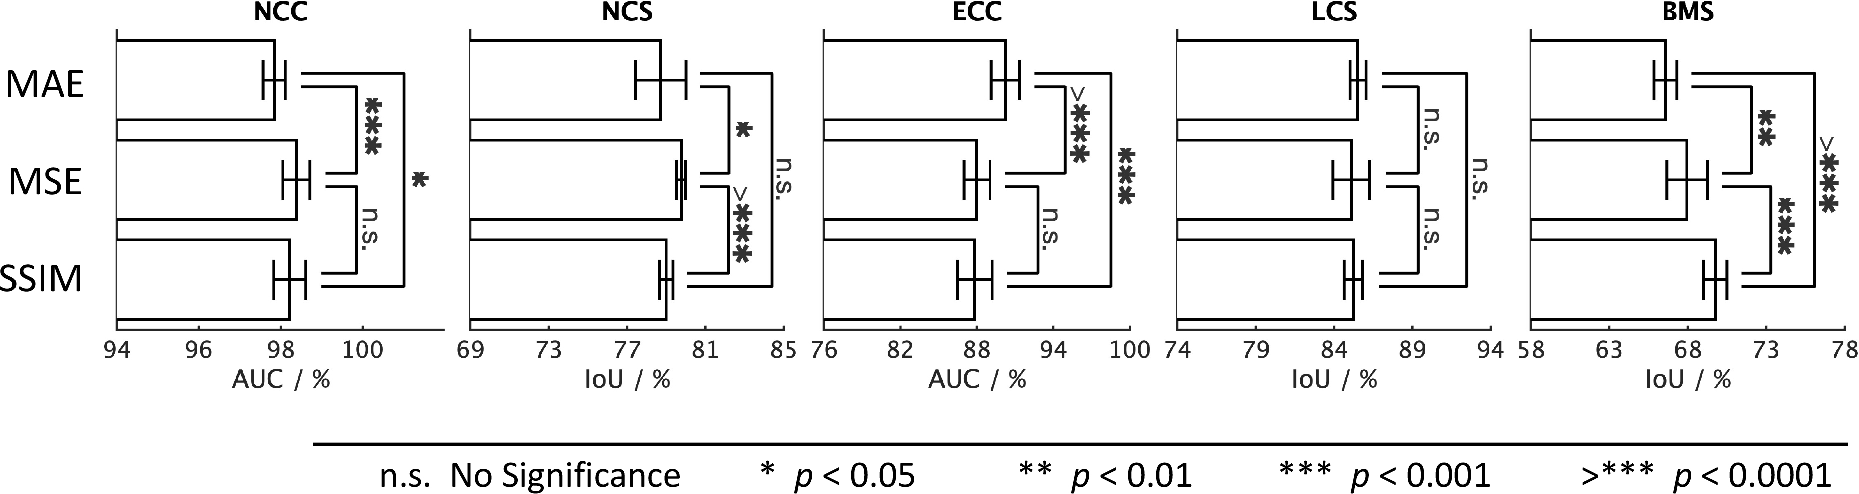
\includegraphics[width=0.9\columnwidth]{Figures/CH5/fig_losses.pdf}
\caption[Assessment the Restoration Loss and Model Transferability]{
We compare three different losses for the task of image restoration. There is no evidence that the three losses have a decisive impact on the transfer learning results of five target tasks. Note that for this ablation study, all the proxy and target tasks are implemented in PyTorch.
}
\label{ch5:fig:losses}
\end{center}
\end{sidewaysfigure}

% \fillandplacepagenumber
% \end{landscape}
%%%%%%%%%%%%%%%%%%%%%%%%%%%%%%%%%%%%%%%%%%%%

\begin{figure}[t]
\centering
\includegraphics[width=1.0\linewidth]{Figures/CH5/fig_image_restoration.pdf}
\caption[Models Genesis Can Detect Infected Regions from Images]{
Examples of image restoration using Genesis Chest CT. We pass unseen CT images (Column 1) to the pre-trained model, obtaining the restored images (Column 2). The difference between input and output has been shown in Column 3. In most of the normal cases, such as those in Rows 1---2, Genesis Chest CT can perform a fairly reasonable identical-mapping. Meanwhile, for some cases that contain opacity in the lung, as illustrated in Row 3, Genesis Chest CT tends to restore a clearer lung. As a result, the diffuse region is revealed in the difference map automatically. We have zoomed in the region for a better visualization and comparison.
}
\label{ch5:fig:image_restoration}
\end{figure}
    
    
\subsection{Does Better Restoration Transfer Better?}
\label{ch5:restoration_loss}

Our transfer learning results in Sec.~\ref{ch5:experiments} suggest that image restoration is a promising task to learn generic 3D image representation. This also means that image restoration quality has an implicit correlation with model transferability to some extent. To assess restoration quality, we compare the Mean Square Error (MSE) loss with other commonly used loss functions for image restoration\footnote{I acknowledge Jiaxuan Pang, with whom I co-authored~\citet{zhou2019models,zhou2021models}, for implementing Models Genesis in PyTorch version with Vatsal Sodha; Shivam Bajpai and Jiaxuan Pang for comparing three loss functions of the proxy task.}, such as Mean Absolute Error (MAE) and Structural Similarity Index (SSIM)~\citep{wang2004image}. All of them compute the distance between input and output images, while SSIM concentrates more on the restoration quality in terms of structural similarity than MSE and MAE. Since the publicly available 3D SSIM loss was implemented in PyTorch\footnote{\label{foot:ssim}SSIM loss in 3D: \href{https://github.com/jinh0park/pytorch-ssim-3D}{https://github.com/jinh0park/pytorch-ssim-3D}}, to make the comparisons fair, we have adapted our five target tasks into PyTorch as well. 
\figurename~\ref{ch5:fig:losses} shows mixed performances of the five target tasks among the three alternative loss functions. As discussed in Sec.~\ref{ch5:transformation_augmentation}, the ideal loss function for representation learning is one that can explicitly determine the power of image representation. However, the three losses explored in this section are implicit, based on the premise that the image restoration quality can indicate a good representation. 
Further studies with restoration quality assessment and its relationship to model transferability are therefore suggested.



\subsection{Can Models Genesis Detect Infected Regions from Images?}
\label{ch5:disease_detection}

Genesis Chest CT has been pre-trained using 623 CT images in the LUNA~2016 dataset. To assess the image restoration quality, we utilize the rest of the 265 CT images from the dataset and present examples in \figurename~\ref{ch5:fig:image_restoration}. Specifically, we pass the original CT images to the pre-trained Genesis Chest CT. To visualize the modifications, we have further plotted the difference maps by subtracting the input and output. Since the input images involve no image transformation, most of the restored CT scans (see Rows~1---2) can preserve the texture and structures of the input images, only encountering few changes thanks to the identical-mapping training scheme and the skip connections between encoder and decoder. Nonetheless, we observe some failed cases (see Row~3), especially when the input CT image contains diffuse disease, which appears as an opacity in the lung.
Genesis Chest CT happens to ``remove'' those opaque regions and restore a much clearer lung. This may be due to the fact that the majority of cropped sub-volumes are normal and are being used as ground truth, which empowers the pre-trained model with capabilities of detecting and restoring ``novelties'' in the CT scans. More specifically, in our work, these novelties include abnormal intensity distribution injected by non-linear transformation, atypical texture and boundary injected by local-shuffling, and discontinuity injected by both inner and outer cutout. Based on the surrounding anatomical structure, the model predicts the opaque area to be air, therefore restoring darker intensity values. This behavior is certainly a ``mistake'' in terms of image restoration, but it can also be thought of as an attempt to detect diffuse diseases in the lung, which is challenging to annotate due to their unclear boundary. By training an image restoration task, the diseased area will be revealed by simple \textit{subtraction} of the input and output. More importantly, this suggested detection approach requires zero human annotation, neither image-level label nor pixel-level contour, contrasting from the existing weakly supervised disease detection approaches~\citep{zhou2016learning,baumgartner2018visual,cai2018iterative,siddiquee2019learning}.


\subsection{Conclusion and Broader Impacts}
\label{ch5:discussion_conclusion:conclusion_broader_impacts}

A key contribution of ours is a collection of \textit{generic source} models, nicknamed Models Genesis, built directly from {\em unlabeled} 3D imaging data with our novel unified self-supervised method, for generating powerful application-specific \textit{target} models through transfer learning. While the empirical results are strong, surpassing state-of-the-art performances in most of the applications, our goal is to extend our Models Genesis to modality-oriented models, such as Genesis MRI and Genesis Ultrasound, as well as organ-oriented models, such as Genesis Brain and Genesis Heart. We envision that Models Genesis may serve as a primary source of transfer learning for 3D medical imaging applications, in particular, with limited annotated data. 
To benefit the research community, we make the development of Models Genesis open science, releasing our codes and models to the public. 
Creating all Models Genesis, an ambitious undertaking, takes a village; therefore, we would like to invite researchers around the world to contribute to this effort, and hope that our collective efforts will lead to the holy grail of Models Genesis, all powerful across diseases, organs, datasets, specialties, and modalities.

We first presented Models Genesis in our MICCAI 2019 paper~\citep{zhou2019models}. This paper received the MICCAI Young Scientist Award and was the Finalist for the Best Presentation Award. Models Genesis have also been chosen as one of the select contributions and received the MedIA Best Paper Award in Medical Image Analysis. This technique has been adopted for various medical imaging applications, such as lymph node classification in histopathology images~\citep{xu2020data}, COVID-19 classification in CT images~\citep{sun2020context}, brain hemorrhage classification in CT images~\citep{zhu2020aggregative}, Alzheimer's disease classification in MR images~\citep{zhang2020universal}, blood cavity segmentation in MR images~\citep{zhang2020universal}, and so on. In addition, we believe that Models Genesis would be of potential for remote sensing, given the capability of our self-supervised method learning recurrent anatomical patterns and the availability of wealthy geographical information naturally associated with satellite images.



% \section*{Acknowledgements}

% I thank Zuwei Guo for implementing Rubik's Cube~\citep{zhuang2019self} and the 3D version of Jigsaw~\citep{noroozi2016unsupervised} and DeepCluster~\citep{caron2018deep}; Fatemeh Haghighi and Mohammad Reza Hosseinzadeh Taher for implementing the 3D version of in-painting~\citep{pathak2016context}, patch-shuffling~\citep{chen2019self}, and working with Zuwei Guo in evaluating the performance of MedicalNet~\citep{chen2019med3d}; Md Mahfuzur Rahman Siddiquee for examining NiftyNet~\citep{gibson2018niftynet} with our Models Genesis; Pengfei Zhang for comparing two additional random initialization methods with our Models Genesis; Shivam Bajpai for comparing three loss functions of the proxy task; Nima Tajbakhsh for revising our conference paper; Jae Y. Shin for organizing and pre-processing the PE dataset; Ruibin Feng for valuable discussions; and Keerthi Shrikar Tatapudi for helping improve the writing of this paper.
\chapter{Interpreting Medical Images}
\label{ch6}

In modern medical practice, medical image interpretation has largely been conducted by human experts such as radiologists and other physicians. However, owing to the wide variety of medical pathology that may affect human beings, the limitations of human perception, and human fatiguability, an increasing role for computer-aided diagnosis (CAD) in medicine has been recognized. In the past few years, the interest in artificial intelligence has mushroomed within medical image interpretation, driven primarily by remarkable advances in deep learning. As discussed in the previous chapters, advancements in the fields of active learning, model designing, and self-supervised learning have found a myriad of applications in medical image analysis, propelling it forward at a rapid pace. Computers naturally excel at discovering and recognizing intricate patterns from images while also providing quantitative assessments for medical imaging. As a result, CAD systems can overcome human limitations affecting medical image interpretation, allowing physicians to focus more on analytical interpretation tasks. This chapter introduces several distinctive characteristics of medical images, pressing clinical needs for imaging technologies, and existing medical applications.

\section{Characteristics of Medical Images}
\label{ch6:characteristics}

Medical images possess particular characteristics compared with natural images, providing unique opportunities for the application of computer-aided techniques to assist in medical diagnosis. Such particular characteristics provide the basis for imaging research advances that have subsequently been translated into clinically usable products. Below we summarize some of the most distinguished imaging characteristics and discuss how they are exploited to advance computer-aided diagnosis in medical imaging.

\begin{enumerate}
    
    \item \textit{Medical images are created by modalities.} Natural images typically consist of 3-channel (Red, Green, and Blue) images that exist in the visible light spectrum, whereas various modalities are used to create medical images, including computed tomography (CT), magnetic resonance imaging (MRI), positron emission tomography (PET), mammography, ultrasound, radiography, and so on. Each modality uses a portion of the non-visible electromagnetic spectrum (with the exception of ultrasound, which employs sound waves for image creation) to create images for visualizing and identifying certain medical disorders and procedural complications. Certain medical imaging modalities are more conducive for the evaluation of particular disorders than others. For example, abnormalities such as acute active hemorrhage are more readily diagnoseable by intravenous contrast-enhanced CT than MRI, whereas small or subtle lesions such as prostate cancer, uterine cancer, and metastases to the bone and brain may be better shown by MRI. Also, although they may often require the use of ionizing radiation or intravenous contrast administration, cross-sectional techniques, such as CT and MRI, are capable of producing images with substantially richer details than radiography (often colloquially referred to as ``X-rays'').
    
    \item \textit{Medical images possess high dimensionality.} Cross-sectional imaging techniques, such as CT, MRI, and ultrasound, produce three-dimensional images, and when dynamic imaging is performed, a fourth dimension---time---is added. While the world around us is three dimensional, human eyesight is essentially a two-dimensional process. Although various reconstruction algorithms essentially ``simulate'' the 3D world from multiple 2D views, human eyesight nevertheless relies on two-dimensional spatial information processing. When reading a volumetric cross-sectional imaging examination, radiologists must scroll through a stack of images back to mentally ``reconstruct''  the underlying anatomy in three dimensions. This is cumbersome and time-consuming, especially when searching for small lesions, which are only seen on a few images within a large volumetric stack of images, and particularly when an abnormality is similar in appearance to normal anatomies, such as a small lung nodule (which can closely resemble normal pulmonary vessels). To avoid overlooking potentially significant abnormalities, radiologists must scrutinize all aspects of each image contained within a large volumetric stack; nevertheless, it has been well-established through eye-tracking perceptual research that even trained observers fail to visually scan all parts of a medical image~\citep{rubin2015characterizing}. In contrast, computer algorithms can interpret high-dimensional images the same way as 2D images by directly harnessing spatial and temporal information. 
    
    \item \textit{Medical images vary in quality.} Owing to substantial differences among medical imaging equipment manufacturers as well as variable proprietary hardware and software platforms, medical images may vary in quality and content among various institutions as well as within a given institution. Furthermore, acquisition protocol parameters (of which there are numerous considerations that must be addressed for a given application), frequently vary considerably among institutions, even for a given manufacturer and application. Such variability results in ``domain gaps'', both in terms of quality and technical display. These domain gaps are regarded as a major obstacle to the development of robust deep learning methods, often referred to as ``domain shift'' or ``distribution drift''. For example, CT scans performed using 5 mm slice thickness can handicap a model trained using CT scans performed using a 0.75 mm thickness, resulting in deep learning methods with a limited clinical value. While the domain shift problem can be addressed by a universally applied configuration for acquiring medical images across hospitals, such a requisite is unlikely to be adopted. Approaches such as semi-supervised learning, domain adaptation, and federal learning have been explored to address the ``domain shift'' problem.
    
    \item \textit{Medical images convey physical meaning.} The color information in natural images does not usually carry categorical meaning. For instance, a shirt is a shirt no matter what color it is. In contrast, the exact or relative pixel intensity value in a given medical image corresponds to a specific constituent within the human body, particularly for cross-sectional imaging modalities such as CT and MRI. CT images are created by directing ionizing radiation through a body part and counting the relative number of photons absorbed by the tissue traversed by the x-ray beam---a greater number of photons absorbed occurs with denser tissue, such as bone, whereas a greater number of photons transmitted (not absorbed and thus reaching the detector) occurs with less dense tissue, such as lung parenchyma. The commonly used scale to represent the relative amount of X-ray photon absorption at CT is the Hounsfield Units (HU) and reflects tissue density. By convention, an attenuation coefficient of 0 HU is equivalent to the density of water (1 gm/cm$^3$). Air or gas, as may be encountered within the large airways and bowel, has an attenuation coefficient of -1,000 HU, whereas bone, a very dense structure, has an attenuation coefficient of approximately 1000 HU. Other tissues within the human body have attenuation coefficients within this range. For example, fat has a value between -80 and -30 HU, whereas unenhanced muscle has an attenuation coefficient ranging between 35 and 55 HU. This ability to directly measure the density of human tissue enables human experts and computer algorithms to identify both normal human anatomy as well as potential abnormalities. More importantly, the semantics embedded in the pixel intensity is a weak annotation that can be harnessed to facilitate the model to learn the appearance of anatomic structures without extensive manual annotation.
    
    \item \textit{Medical images encode relative location and orientation.} When identifying objects from natural images, their locations are generally not important: a cat is a cat no matter if it appears in the top left or bottom right of the image. In contrast, in medical imaging, the relative location and orientation of a structure and the intrinsic consistency of anatomical relationships are important characteristics that allow recognition of normal anatomy and pathological conditions. The regular and predictable location of various structures in the human body is a valuable characteristic for training deep learning models. Since medical imaging protocols snap patients in fairly consistent and reproducible positions, these methods generate images with great similarity across various equipment manufacturers and facility locations. Therefore, recognizing the stereotypical position and orientation information of human anatomy provides an opportunity to reduce false positive results and improve the accuracy of disease detection and segmentation. Several works have demonstrated the value of this approach by adding location features, modifying objective functions, and constraining coordinates relative to landmarks in images. For instance, employing ultrasound for measurement of carotid arterial intimal-medial thickness for cardiovascular risk stratification, the measurement could be performed at any point along the longitudinal aspect of the vessel, and such variability could adversely affect results and reproducibility. However, it is standard practice to perform this measurement  1 cm beyond a recognizable anatomic landmark---the carotid bulb~\citep{stein2008use}. As a result, the anatomically recognizable carotid bulb provides a contextual constraint for training deep learning methods. 
    
    \item \textit{Medical images encode both scale and distance.} The uncertain distance between camera and object limits precise size measurements in natural images; in contrast, the physical size of a structure is preserved in medical images. Scale is one of the quantitative attributes of standard imaging formats. The size of a pixel in CT, as an example, is often specified in the DICOM header. By obtaining the number of pixels belonging to an object and the pixel scale from the header, the physical scale and distance between normal structures and lesions in the image can easily be computed. This information is a critical feature in the assessment of disease, both by human interpretation and computer-aided diagnosis because the physical size of a lesion influences disease stage, treatment options, and prognosis. Moreover, the lesion size distribution can serve as a statistic to estimate the domain gaps among datasets collected from different equipment manufacturers, facilities, and regions, allowing the creation of more robust models and enhancing the ability to extrapolate computer-aided diagnoses across various medical practices.
    
    \item \textit{Medical images have sparse and noisy labels.} Unlike natural imaging datasets, it is impractical to annotate millions of medical images with a systematic label hierarchy. Most publicly available medical imaging datasets focus on particular anatomic regions and only provide annotation for the object of interest. For example, the KiTS dataset provides annotation only for the kidney, the LiTS dataset for the liver, and the NIH Pancreas-CT dataset for the pancreas. There is no dataset that provides systematic annotation for all visible structures in a medical imaging dataset; existing annotated datasets are either only partially annotated or only annotated on a small scale. Organizing a hierarchical labeling dictionary to address various organs, tissues, and diseases, as well as reflect their spatial relationships in the human body, remains a large limitation for deep learning methods. Moreover, the available annotated images are often associated with noise due to inter-observer and intra-observer variability. That is, different human experts can provide conflicting opinions regarding a given lesion, reflecting inter-observer variability; furthermore, the same expert is likely to produce very different lesion contours over multiple attempts separated in time, reflecting intra-observer variability. Additionally, more severely noisy labels occur if the abnormality has indistinct boundaries, such as diffuse lung diseases. The partial and imperfect annotation compromises model training and results in ambiguous and unreliable results when deep learning methods undergo testing. 

\end{enumerate}


In summary, medical images contain quantitative imaging characteristics---the intensity value and physical size of pixels---that can be used as additional information to enhance deep learning performance. Medical images also present qualitative imaging characteristics---consistent and predictable anatomical structures with great dimensional details---that can provide an opportunity for comprehensive model training. Nevertheless, several characteristics unique to medical images create unmet challenges, such as isolated, discrepant data and partial, noisy labels, that must be addressed through additional investigation.


\section{Clinical Needs}
\label{ch6:clinical_needs}

Computer-aided diagnosis holds a long history, which has been focusing on a key promise: CAD systems are not developed to replace physicians but rather to enhance their capabilities through computer-physician synergy. With deep learning methods elevating numerous CAD systems to human-level precision, the number of clinical needs has been rapidly increasing in recent decades.

\begin{itemize}
    \item \textit{Medical image classification} refers to classifying what type of lesion is contained in an image. Such classification may be binary (\eg benign or malignant) or multi-class (various types of lesions). The annotation for classification tasks is to assign one or a few labels to an image or a study.
    
    \item \textit{Disease localization and detection} refer to identifying the location of specific lesions. Their difference is subtle: localization aims to locate a single lesion, while detection aims to find all lesions in the image. The annotation for detection and localization provides both the specific location and the scale of the disease with a bounding box.
    
    \item \textit{Medical image segmentation} refers to creating a pixel-wise mask of the organ/lesion in the image. Segmentation can ease the analysis by measuring more accurate and desirable imaging biomarkers. The annotation for segmentation tasks is to assign every pixel in an image to at least one class.
    
    \item \textit{Medical image registration} refers to aligning the spatial coordinates of one or more images into a standard coordinate system. Image registration plays an important role in disease prognosis by establishing correspondence among multiple scans taken from different time points. 
    
    \item \textit{Medical image reconstruction} refers to producing images suitable for human interpretation from raw data obtained by imaging devices, such as CT or MRI scanners. A fast and high-quality radiological image reconstruction will substantially reduce radiation exposure and doses of intravenous contrast material.
    
    \item \textit{Medical image enhancement} refers to adjusting the intensity of an image for better visualization or further analysis. Such enhancement includes denoising, super-resolution, artifact removal, MR bias field correction, and image harmonization.
    
    \item Other tasks include: \textit{landmark detection}, \textit{image or view recognition}, \textit{automatic report generation}, etc.

\end{itemize}


In this dissertation, we mainly focus on the tasks of image classification and segmentation, with some other clinical needs such as disease detection and CIMT thickness measurement. Our goal is to minimize the annotation cost associated with these tasks while maintaining comparable or even higher performance. We have further elaborated on the specific imaging datasets in Appendix~\ref{ap1}.





\section{Medical Application: A Case Study of PE CAD}
\label{ch6:medical_applications}

Interest in implementing deep learning methods in computer-aided diagnosis systems has increased tremendously in the past decade due to the promising, or even super-human, performance for various medical applications. This section provides a case study for conducting a medical application that involves deep learning, from curating the structure of data and annotation, to developing the system and validating the performance. Specifically, the objective is to demonstrate the annotation-efficiency of our devised techniques in several key facets of the CAD system in practice. We illustrate the step-by-step workflow using the application of detecting pulmonary embolism from CTPA scans. The idea of implementing deep learning methods into computer-aided diagnosis systems can be adapted to many other medical applications that require automated medical image analysis.

%##############################################################################################
\begin{figure}[t]
\begin{center}
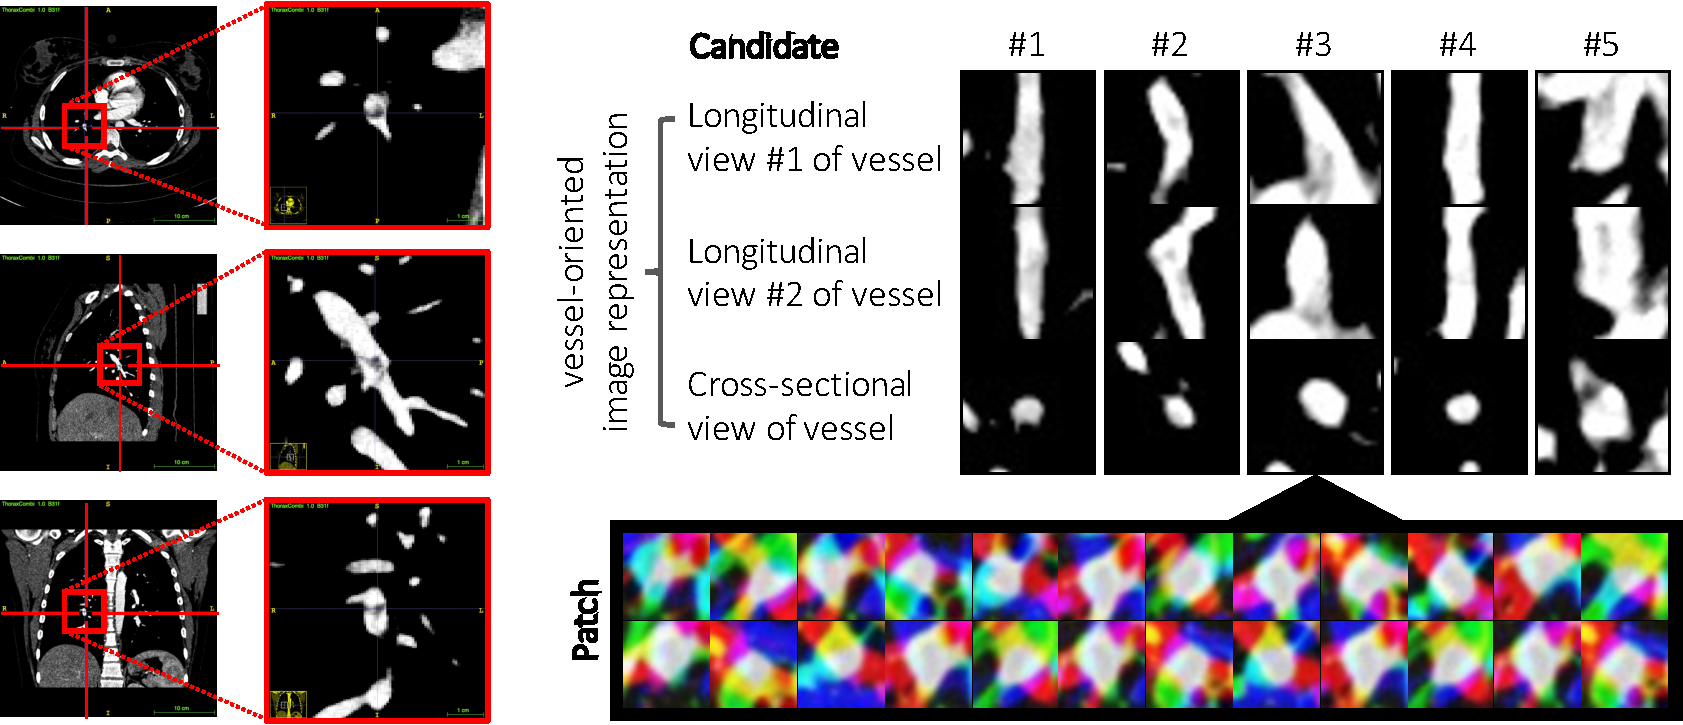
\includegraphics[width=1.0\linewidth]{Figures/CH6/fig_pe_visualization.pdf}
\end{center}
\caption[Examples of Pulmonary Embolism in CTPA Images]{(a) The typical appearance of pulmonary embolism in the CTPA scan, presented from an axial, coronal, and sagittal views. (b) Five different pulmonary embolism candidates in the vessel-oriented image representation~\citep{tajbakhsh2015computer}. It was adopted in this work because it achieves great classification accuracy and accelerates CNN training convergence.}
\label{ch6:fig:pe_visualization}
\end{figure}
%##############################################################################################

\subsection{Pulmonary Embolism}
\label{ch6:medical_applications:pe_introduction}

Pulmonary Embolism (PE) is a major national health problem, which is responsible for 100,000$\sim$200,000 deaths annually in the United States~\citep{pauley2019age}, representing the third most common cause of cardiovascular death after myocardial infarction and stroke~\citep{martin2020time}. A PE is a condition in which a thrombus (often colloquially referred to as a ``blood clot'') travels to the lungs, often from a lower extremity venous source, producing a blockage of the pulmonary arteries within the lungs. The mortality rate of untreated PE may approach 30\%~\citep{calder2005mortality}, but it decreases to as low as 2\% with early diagnosis and appropriate treatment~\citep{sadigh2011challenges}. CT pulmonary angiography (CTPA) is the primary means for PE diagnosis, wherein a radiologist carefully traces each branch of the pulmonary artery for any suspected PEs. PEs appear as ``filling defects'' within enhanced pulmonary arteries following the administration of intravenous contrast, as shown in~\figureautorefname~\ref{ch6:fig:pe_visualization}(a). However, CTPA interpretation is a time-consuming task, of which accuracy depends on human factors, such as attention span and sensitivity to the visual characteristics of PEs. Computer-aided PE detection can have a major role in improving the diagnostic capability of radiologists and decreasing the reading time of CTPA scans.

We developed our computer-aided PE detection system by using an in-house dataset from ASU-Mayo~\citep{tajbakhsh2019computer}, which consists of 121 CTPA scans with a total of 326 emboli\footnote{I thank Jae Y. Shin for organizing and pre-processing the PE dataset.}. The dataset provides the spatial coordinates of each emboli in the scan. The dataset is divided at the patient-level into a training set (71 patients) and a test set (50 patients). To study the robustness and generalizability of the algorithm, we have also evaluated our system using 20 CTPA scans from the CAD-PE competition\footnote{\href{http://www.cad-pe.org/}{http://www.cad-pe.org/}}. Our computer-aided PE detection system consists of two stages to detect PEs from images: (1) candidate generation and (2) false positive reduction. These two stages have also been widely used in most existing disease detection systems. In the following sections, we describe the methodology and performance for each stage in detail.





\subsection{Generating Pulmonary Embolism Candidates}
\label{ch6:medical_applications:candidate_generation}

We use an unsupervised approach for candidate generation, consisting of heuristic lung segmentation and the tobogganing algorithm~\citep{fairfield1990toboggan}. In a chest CTPA scan, lungs appear darker than their surrounding. To segment lungs from the scan, we first clip voxel intensity values using a threshold of -400, resulting in a binary volume wherein the lungs and other dark regions appear white. Then, we perform a closing operation to fill all dark holes in the white area. To exclude non-lung areas, we perform a 3D connected component analysis and remove the components with small volumes or a large length ratio between the major and minor axes. The purpose of segmenting the lungs is to reduce the computational time and the number of false positives for the toboggan algorithm. Since peripheral PEs only appear in pulmonary arteries, there is no need to search for PE candidates outside the lungs. The tobogganing algorithm is then applied only to the lung area, generating the PE candidate coordinates that we will then use to crop sub-volumes from the CTPA scan. This procedure of candidate generation was firstly designed by~\citet{tajbakhsh2015computer}. 


We directly applied their PE candidate generator to the dataset, resulting in a total of 8,585 PE candidates, wherein 863 were true positives and 7,722 were false positives. There are 326 unique emboli annotated in our dataset. Since multiple detections can be generated from a large PE, the number of true positives is greater than the number of unique emboli. \citet{tajbakhsh2015computer} reported a sensitivity of 93\% with, on average, 65.8 false positives per patient for the entire candidate generation stage.


\begin{table}[t]
\centering
\footnotesize
\caption[Models Genesis with 3D VOIR Perform the Best in PE Detection]{
We evaluate vessel-oriented image representation (VOIR)~\citep{tajbakhsh2019computer} in comparison with 2D, 2.5D, and 3D solutions for the task of reducing PE false positives. Our comprehensive experiments have demonstrated that: (1) the vessel-oriented image representation exceeds the regular image representation; (2) 3D volume-based inputs offer higher performance than 2.5D orthogonal inputs, which in turn work better than 2D slice-based inputs; (3) Models Genesis consistently outperform models learning from scratch. Overall, the best performance is obtained by Models Genesis trained with 3D volume-based VOIR inputs. The entries in bold highlight the best results achieved by different model input formations. All of the results in the table are candidate-level AUC (Area Under the ROC Curve), including the mean and standard deviation (mean$\pm$s.d.) across ten trials.
}
\label{ch6:tab:voir_nonvoir}
\begin{tabular}{p{0.29\linewidth}P{0.2\linewidth}P{0.2\linewidth}P{0.2\linewidth}}
    \hline
    Task: \texttt{ECC} (w/o VOIR) & Random & Models ImageNet & Models Genesis \\
    \hline
    2D slice-based input & 60.33$\pm$8.61 & 62.57$\pm$8.04 & \textbf{62.84$\pm$8.78} \\
    2.5D orthogonal input & 71.27$\pm$4.64 & \textbf{78.61$\pm$3.73} & 78.58$\pm$3.67 \\
    3D volume-based input & 80.36$\pm$3.58 & n/a & \textbf{88.04$\pm$1.40} \\
    \hline
    Task: \texttt{ECC} (w/t VOIR) & Random & ImageNet & Genesis \\
    \hline
    2D slice-based input & 86.16$\pm$1.94 & 86.83$\pm$0.97 & \textbf{87.43$\pm$1.34} \\
    2.5D orthogonal input & 87.29$\pm$3.25 & 88.04$\pm$0.78 & \textbf{88.32$\pm$1.70} \\
    3D volume-based input & 92.01$\pm$0.98 & n/a & \textbf{92.81$\pm$0.47} \\
    \hline
    \end{tabular}
\end{table}


\subsection{Reducing Pulmonary Embolism False Positives}
\label{ch6:medical_applications:false_positive_reduction}

The previous stage generates coordinates that indicate where the PE candidate is located. We crop sub-volumes based on the location, so that the PE candidate will appear in the center of each sub-volume. The sub-volume has a physical size of 20$\times$20$\times$20 mm and then resized into 64$\times$64$\times$64 pixel. To conduct a fair comparison with the prior studies~\citep{zhou2017fine,tajbakhsh2016convolutional,tajbakhsh2019computer}, we compute candidate-level AUC (Area Under the ROC Curve) for classifying true positives and false positives. 


Compared with \citet{tajbakhsh2019computer}, we have advanced the methodology and yielded significant performance gains in three aspects (see~\tableautorefname~\ref{ch6:tab:voir_nonvoir}).

\begin{enumerate}

    \item \textit{Extending VOIR into the 3D version.} 
    In general, emboli can affect pulmonary arteries in any orientation, exhibiting a significant variation in PE appearance (see~\figureautorefname~\ref{ch6:fig:pe_visualization}(a)). This complicates the classification task and hinders the effective utilization of deep learning methods. To implement vessel alignment, we first apply principal component analysis (PCA) to voxel intensities for estimating the vessel's orientation. Then, we rotate scan planes in alignment with the vessel longitudinal axis, resulting in images with standardized appearance, wherein emboli consistently appear as elongated structures in the longitudinal vessel view and as circular structures in the cross-sectional view (see~\figureautorefname~\ref{ch6:fig:pe_visualization}(b)). This interpolation scheme guided by the vessel axis has the effect of maximally revealing the filling defects, thereby facilitating PE diagnosis for both radiologists and computers. We have implemented VOIR in both 2D (following~\citet{tajbakhsh2019computer}) and 3D\footnote{I thank Douglas Amoo-Sargon for implementing 3D VOIR in the PE dataset.}, demonstrating that the vessel-oriented image representation exceeds the regular image representation.
    
    \item \textit{Utilizing three-dimensional models and data.}
    While adopting 3D models to process 3D volumetric data may appear to be a natural choice, it occurs at a substantial computational cost, lack of sufficient data, and risk of overfitting. As a result, several alternative strategies were proposed to reformat 3D applications into 2D problems. For instance, \citet{ben2016fully,sun2017multiphase} formulated regular 2D inputs by extracting adjacent axial slices (refer to as 2D slice-based input). A more advanced strategy, presented in~\citet{prasoon2013deep,roth2014new,roth2015improving}, is to extract axial, coronal, and sagittal slices from volumetric data (refer to as 2.5D orthogonal input). These reformatted 2D solutions can generate a large number of data and benefit from 2D pre-trained ImageNet. However, 2D solutions inevitably sacrifice the rich spatial information in 3D volumetric data and large capacity of 3D models. As the computer power increased and pre-trained 3D models developed in recent years, the interest is shifting back to 3D techniques, with several emerging evidences~\citep{zhou2021models,isensee2021nnu} indicating that 3D applications are better to be addressed in 3D. Our experimental results also suggest that, with the same initialization and vessel orientation, 3D volume-based inputs offer higher performance than 2.5D orthogonal inputs, which in turn work better than 2D slice-based inputs.
    
    \item \textit{Initializing models with Models Genesis.}
    Training a deep model from scratch is difficult because it requires a large amount of labeled training data and a great deal of expertise to ensure proper convergence. Fine-tuning Models ImageNet has become the most practical adoption for deep learning applications in medical imaging to ease the training procedure~\citep{shin2016deep,tajbakhsh2016convolutional}. On the other hand, Models ImageNet may give suboptimal initialization in the medical imaging domain~\citep{raghu2019transfusion}, as they were pre-trained from only natural images; it is associated with a large domain gap for medical images. We pre-train Models Genesis in the same domain to reduce this domain gap. Our Models Genesis 2D offer similar performance to Models ImageNet. This result is encouraging because our Models Genesis 2D were developed without using any manual annotation, while Models ImageNet demand more than fourteen million annotated images. More importantly, Models ImageNet only provide 2D models, which cannot handle 3D data directly, while Models Genesis can be pre-trained in both a 2D and 3D manner. Our results show that Models Genesis secure great performance gain (10\% improvement without VOIR and 4\% with VOIR) in comparison with Models ImageNet. Overall, we conclude that Models Genesis consistently outperform models learning from scratch and achieve the best performance when using 3D VOIR sub-volumes as input.
    
    
\end{enumerate}



%%%%%%%%%%%%%%%%%%%%%%%%%%%%%%%%%%%%%%%%%%%%
% \begin{landscape}
% \thispagestyle{empty}

\begin{sidewaysfigure}
\begin{center}
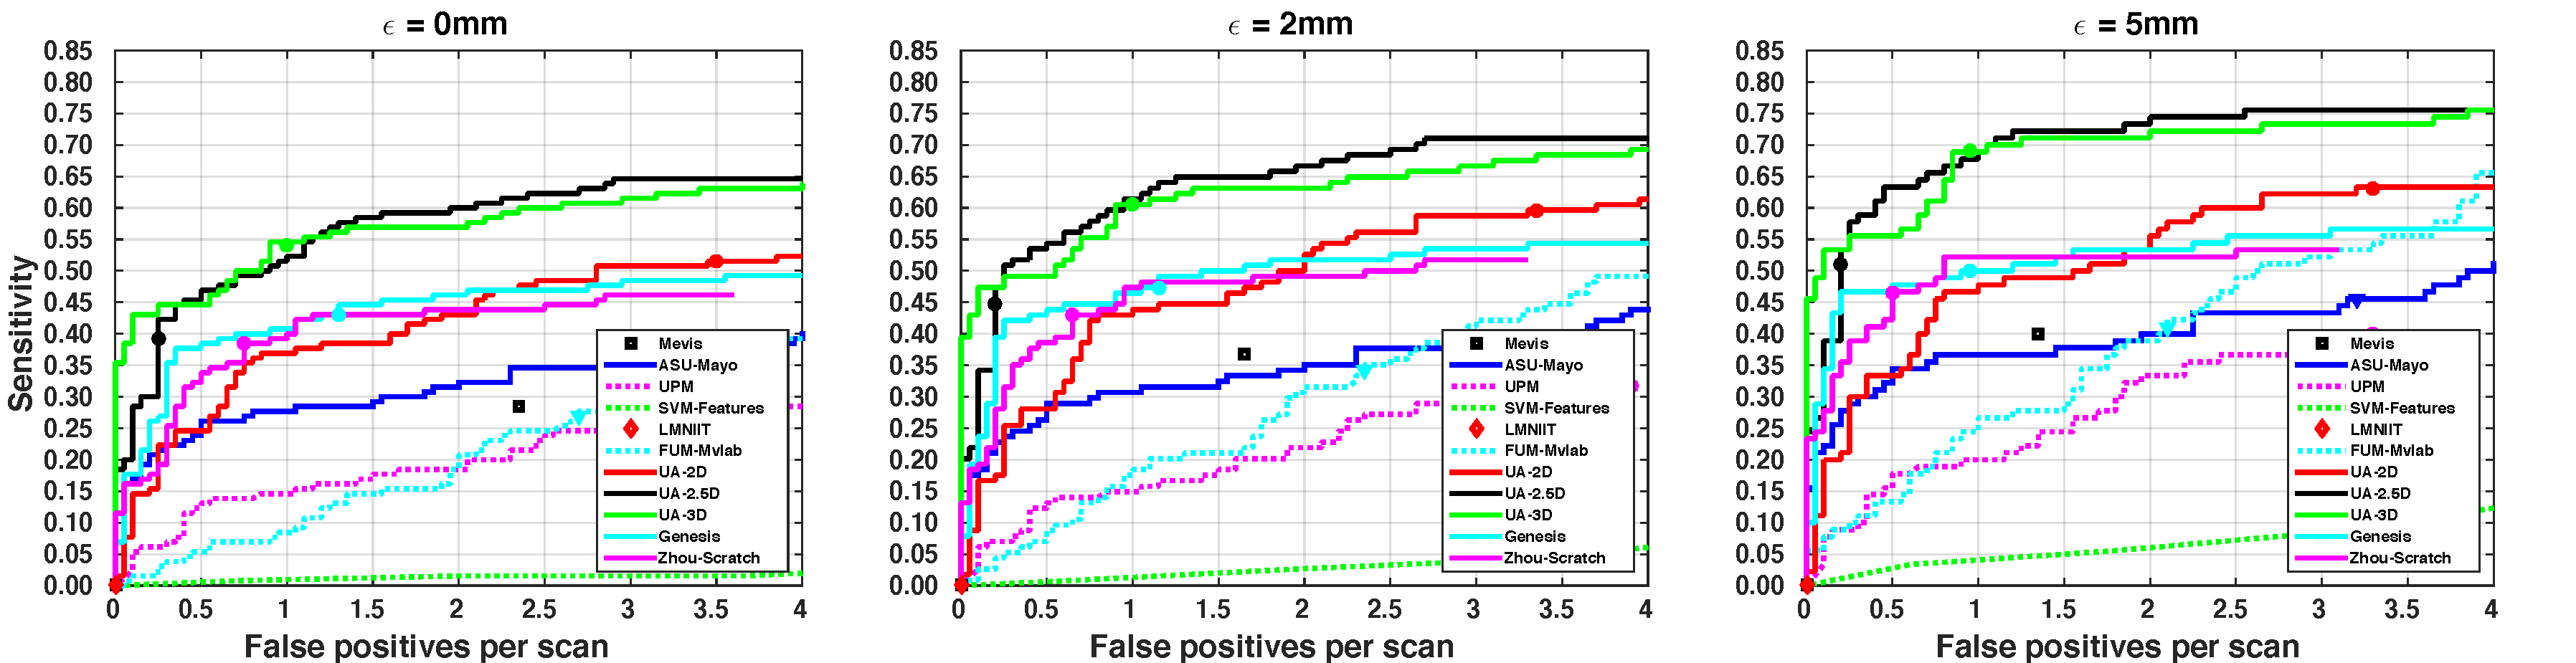
\includegraphics[width=1.0\columnwidth]{Figures/CH6/fig_pe_cad.pdf}
\end{center}
\caption[Comparison of Our PE CAD System with the State of the Arts]{
We have compared the top participating teams of the CAD-PE competition~\citep{gonzalez2020computer}. For each method, the Free‐Response Operating Characteristic (FROC) curves are plotted. 
Our PE CAD was directly evaluated on the 20 CTPA test scans, without using any training scans provided by the competition. 
$\epsilon$ denotes the localization error. That is, a detection is considered a true positive as long as the detection falls within $\epsilon$ distance from the ground truth for PE. The performance at $\epsilon$ = 0 mm provides greater benefits for clinical applications than at 2mm and 5 mm. As reported, our PE CAD (\texttt{Genesis}) is ranked third among the participating teams, achieving a sensitivity of 46\% at 2 false positives per scan ($\epsilon$ = 0 mm). 
This sensitivity is substantially higher than our previous method, which holds a sensitivity of 33\%  (\texttt{ASU-Mayo})~\citep{tajbakhsh2019computer}, highlighting the importance of 3D VOIR and Models Genesis for PE detection. 
We should note that the leading solutions (\texttt{UA-2.5D} and \texttt{UA-3D}) have not only been trained on the 20 training scans, but also had access to an extended training dataset with 51 additional CTPA scans. 
Therefore, our PE CAD is reasonably competitive compared to the state of the art. 
}
\label{ch6:fig:pe_cad}
\end{sidewaysfigure}

% \fillandplacepagenumber
% \end{landscape}
%%%%%%%%%%%%%%%%%%%%%%%%%%%%%%%%%%%%%%%%%%%%


\subsection{Comparing with the State of the Art}

To further examine the robustness of our computer-aided PE detection system, we have participated in the CAD-PE competition\footnote{I thank Nima Tajbakhsh and Jae Y. Shin for generating PE candidates from the competition dataset; German Gonzalez Serrano for organizing the CAD-PE competition and evaluating our system with other participating teams.}. All participating teams can use 20 training scans provided by the competition to develop their systems, and the final performance is evaluated on the additional 20 unseen scans. As shown in~\figureautorefname~\ref{ch6:fig:pe_cad}, our system (\texttt{Genesis}) is ranked third among the participating teams. The top two winners of the competition, \texttt{UA-3D} and \texttt{UA-2.5D}, have utilized an extended training set released by the competition organizers; therefore, their systems are significantly better than others. On the other hand, we directly took the unseen test scans to evaluate our system, which was developed even without using the 20 training scans from the competition. As seen, our system's performance is fairly robust to the different datasets. Considering the potential domain gap between the CAD-PE competition and our in-house dataset, we also anticipate a better performance once adapting our system to the CAD-PE training set in the future. The \texttt{ASU-Mayo} was our previous submission, which used the 2D VOIR approach~\citep{tajbakhsh2019computer}, a consistent, compact, and discriminative image representation to improve the perception of PE. Our current system, compared with \citet{tajbakhsh2019computer}, has made three advancements: (1) extending VOIR to the 3D version, (2) utilizing three-dimensional models and data, and (3) initializing models with Models Genesis. Consequently, the enhanced system achieves a significantly higher sensitivity of 46\% at 2 false positives per scan ($\epsilon$ = 0 mm), increasing the sensitivity by over 10\% than the previous system.


\section{Discussion \& Conclusion}
\label{ch6:discussion}

\subsection{What Is the Current State of Clinical PE CAD?}
\label{ch6:discussion:current_state_of_pe_cad}

The computer-aided pulmonary embolism detection is an illustrative example of how deep learning methods have been integrated into clinical image interpretation. With an estimated 180,000 deaths per year in the United States, the rapidly increasing CTPA examinations far exceed the availability of subspecialty trained cardiopulmonary radiologists~\citep{horlander2003pulmonary}. To address the unmet need for interpretation, general radiologists are also assigned to look through some of the examinations.
Accurately interpreting CTPA examinations requires significant training and experience, so the discordance between cardiopulmonary and general radiologists may exceed 25\% if they interpret the same examination~\citep{hutchinson2015overdiagnosis}. Due to inaccurate interpretations, including false-negative studies (failure to detect emboli) and false-positive studies (diagnosing emboli that are not present, or ``overdiagnosis’’), there is a significant risk of morbidity and mortality for patients. 

Deep learning methods have been developed to assist radiologists with the task of PE detection and exclusion. Several studies suggest that radiologists who use current CAD systems can improve the sensitivity from 77$\sim$94\% to 92$\sim$98\%~\citep{das2008computer,wittenberg2011impact,blackmon2011computer,wittenberg2013computed}. 
One particular system, developed by AIDOC medical (Tel Aviv, Israel), has recently been adopted by Mayo Clinic\footnote{I thank Michael B. Gotway for sharing the clinical experience of PE CAD in Mayo Clinic.}. Once a CTPA examination is transferred from the CT scanner to radiologists for interpretation, the system will perform the task of PE detection and exclusion in the backend. This system runs ``silently'' in the background and determines results as either negative or positive for PE. If positive, a pop-up window will localize the embolus for radiologist confirmation. In a study by~\citet{weikert2020automated}, the AIDOC algorithm showed a sensitivity of 92.7\% on a per-patient basis with a false positive rate of 3.8\%, or 0.12 false-positive detection. Most notably, the average processing time for the algorithm was 152 seconds, but typically this processing occurs while the data is being transferred from the CT scanner to the picture archiving communication system. Thus, the images are not completely available for radiologists to review immediately. An additional 25 seconds is required for case uploading~\citep{weikert2020automated}. In practice, the AIDOC system analysis is either complete and ready for review when the study is opened by the radiologist, or the case is being actively processed. The examination is open for interpretation and the results are commonly available before the radiologist completes the review of the study. 
Such a PE CAD system cannot, and was not designed to, substitute the doctor, but it definitely makes radiologists better and faster decision makers, playing a supporting and final interpretative role in medical diagnosis.


\subsection{Conclusion and Broader Impacts}
\label{ch6:discussion_conclusion:conclusion_broader_impacts}

The introduction of deep learning methods in clinical medicine, particularly diagnostic imaging, has rapidly stimulated many medical applications in recent years. In this chapter, several important characteristics of medical images and pressing clinical needs are reviewed to highlight their strengths and limitations. Accordingly, the techniques we devised were mainly inspired by these imaging characteristics, while the medical applications we chose were deeply motivated by the clinical needs. Furthermore, we have presented our end-to-end CAD system for pulmonary embolism detection as an example of how deep learning methods address clinical problems. We have illustrated the annotation efficiency in several key facets of the system and demonstrated our system's robustness in the CAD-PE competition. Numerous other deep learning applications are already available to assist radiologists with interpreting a wide variety of disorders from images, functioning as a ``second reader''. These applications hold promise both for providing increased accuracy through enhanced detection and specificity, and for mitigating the workloads experienced by radiologists due to the rise of advanced imaging techniques. 


% \section*{Acknowledgements}

% I thank Michael B. Gotway for revising this chapter and sharing the clinical experience of PE CAD in Mayo Clinic; Jae Y. Shin for organizing and pre-processing the PE dataset; Douglas Amoo-Sargon for implementing 3D VOIR to the PE dataset; Nima Tajbakhsh for generating PE candidates from the competition dataset; German Gonzalez Serrano for organizing the CAD-PE competition and evaluating our system with other participating teams; Jianming Liang for providing constructive advises.


% \subsection{Acquiring annotations in candidate-level or patient-level?}

% \subsection{Computer-aided diagnosis or automated computer diagnosis?}

% \subsection{What would be the clinically acceptable performance?}

% \subsection{On which aspects can computers impact the most?}

\chapter{Conclusion}
\label{ch7}


Deep learning methods will empower many aspects of computer-aided diagnosis over the next decade, from medical image acquisition and interpretation to clinical decision making~\citep{esteva2019guide,zhou2021review}. Despite the expert human performance of deep learning methods in a few medical applications~\citep{gulshan2016development,esteva2017dermatologist,ardila2019end,mckinney2020international}, its prohibitively high annotation costs raise doubts about their feasibility of applying to those medical specialties that lack such magnitude of annotation. In this dissertation, we have systematically introduced our work in developing annotation-efficient deep learning that enables to (1) smartly identify the most significant subjects to be annotated, (2) effectively aggregate multi-scale image features to maximize the potential of existing annotations, and (3) directly extract medical knowledge from images without manual annotation. We have remarked our contributions in computer-aided diagnosis by supporting several aspects of medical image interpretation, including disease detection, classification, and segmentation. The experimental results on twelve distinct medical applications demonstrate that with a small part of the dataset annotated, we can deliver deep learning methods that match, or even outperform those that require annotating the entire dataset. This observation is encouraging and significant because it addresses the daunting challenge of limited annotated data---the main obstacle standing between deep learning methods and their clinical impact. Our devised methodologies are advantageous on over-represented diseases with abundant existing annotations and also shed new light on many more underrepresented diseases with the deep learning marvel, dramatically reducing annotation costs while maintaining high performance.

More importantly, we have been advocating open access, open data, and open source to benefit the research community. In our dissertation, eight out of the twelve medical applications were taken from publicly available medical imaging benchmarks (elaborated in Appendix~\ref{ap1}), ensuring the reproducibility of the results. Furthermore, we have released the codes and models to the public (detailed in Appendix~\ref{ap2}), making three developed techniques (ACFT, UNet++, and Models Genesis) open science to stimulate collaboration among the research community and to help translate these technologies to clinical practice. We first presented our ACFT, UNet++, and Models Genesis in CVPR~2017, DLMIA~2018, and MICCAI~2019, respectively. They have since been quickly adopted by the research community: reviewed by some of the most prestigious journals and conferences in the field, served as competitive baselines, and enlightened the development of more advanced approaches. Moreover, although our techniques were initially derived from the medical imaging context, their annotation-efficiency and generalizability have been demonstrated by independent research groups from alternative fields, such as text classification~\citep{oftedal2019uncertainty}, vehicle type recognition~\citep{huang2019cost}, streaming recommendation system~\citep{guo2019streaming}, image coloring~\citep{di2021color}, moon impact crater detection~\citep{jia2021moon}, microseismic monitoring~\citep{guo2021first}, etc.


Human annotation is one of the most significant cornerstones for algorithm development and evaluation. For the purpose of development, annotation-efficient deep learning facilitates quick, iterative improvements of the algorithm, whereas for performance evaluating, we still have to curate large, representative annotated datasets. In addition to the sufficient population of patients, we must also evaluate how the algorithms generalize to other medical images acquired from different devices, conditions, and sites---all of which must be annotated---before eventually adopting the techniques into clinical practice. Therefore, the increasing annotation demands are anticipated to continue troubling us with the lack of budget, time, and expertise. Big data is an inevitable trend in the future---with the increasing imaging studies, rising workloads of radiologists, and growing needs for technologies---we embrace the age of big data. The purpose of annotation-efficient deep learning is not to strangle the throat of annotating \textit{per se} but rather to speed up creating such datasets to enable high-performance deep learning methods with a minimal set of human expert annotation efforts. 

% Annotation is important for both training and validation.
% For training, annotation-efficient deep learning can reduce annotation cost.
% But for validation, annotation-efficient deep learning cannot.
% We still need many annotations for validation.
% Big data is inevitable in the future.
% Annotation-efficient is not to stop big data, but helping create big data with small human effort.


%-----------------------back matter
{\singlespace
% Making the references a "part" rather than a chapter gets it indented at
% level -1 according to the chart: top of page 4 of the document at
% ftp://tug.ctan.org/pub/tex-archive/macros/latex/contrib/tocloft/tocloft.pdf
\addcontentsline{toc}{part}{REFERENCES}
\bibliographystyle{asudis}
\bibliography{dis}}
\renewcommand{\chaptername}{APPENDIX}
\addtocontents{toc}{APPENDIX \par}
\appendix
\chapter{Data availability}
\label{ap1}

\newpage

% %%%%%%%%%%%%%%%%%%%%%%%%%%%%%%%%%%%%%%%%%%%%
% \begin{figure}[t]
% %\footnotesize
% \begin{center}
% \includegraphics[width=1.0\linewidth]{Figures/AP1/fig_dataset_annotation.pdf}
% \end{center}
% \caption[Datasets and Annotations Used in This Dissertation]{Datasets and annotations used in this dissertation.}
% \label{ap1:fig:dataset_annotation}
% \end{figure}
% %%%%%%%%%%%%%%%%%%%%%%%%%%%%%%%%%%%%%%%%%%%%

%##############################################################################################
% \begin{landscape}
% \thispagestyle{empty}

\begin{sidewaysfigure}
\begin{center}
\includegraphics[width=1.0\linewidth]{Figures/AP1/fig_dataset_annotation.pdf}
\end{center}
\caption[Datasets and Annotations Used in This Dissertation]{Datasets and annotations used in this dissertation.}
\label{ap1:fig:dataset_annotation}
\end{sidewaysfigure}

% \fillandplacepagenumber
% \end{landscape}
%##############################################################################################


We summarizes the twelve medical imaging applications used in this dissertation, covering lesions/organs from most commonly used medical imaging modalities including microscopy, X-ray, computed tomography (CT), magnetic resonance imaging (MRI), and Ultrasound.

\section*{Lung Nodule False Positive Reduction}
\label{ap1:lung_nodule_classification}

The dataset is provided by LUNA~2016\footnote{\href{https://luna16.grand-challenge.org/}{https://luna16.grand-challenge.org/}}\citep{setio2017validation} and consists of 888 low-dose lung CTs with slice thickness less than 2.5mm. Patients are randomly assigned into a training set (445 cases), a validation set (178 cases), and a test set (265 cases). The dataset offers the annotations for a set of 5,510,166 candidate locations for the false positive reduction task, wherein true positives are labeled as ``1'' and false positives are labeled as ``0''. Following the prior works~\citep{setio2016pulmonary,sun2017automatic}, we evaluate performance via Area Under the Curve (AUC) score on classifying true positives and false positives.

\section*{Pulmonary Embolism False Positive Reduction}
\label{ap1:pulmonary_embolism_classification}

We utilize a database consisting of 121 computed tomography pulmonary angiography (CTPA) scans with a total of 326 emboli. 
Following the prior works~\citep{liang2007computer}, we utilize their PE candidate generator based on the toboggan algorithm, resulting in total of 687 true positives and 5,568 false positives. The dataset is then divided at the patient-level into a training set with 434 true positive PE candidates and 3,406 false positive PE candidates, and a test set with 253 true positive PE candidates and 2,162 false positive PE candidates. To conduct a fair comparison with the prior study~\citep{zhou2017fine,tajbakhsh2016convolutional,tajbakhsh2019computer}, we compute candidate-level AUC on classifying true positives and false positives.


\section*{Chest Disease Classification}
\label{ap1:chestxray}

This is a Chest X-ray dataset that we used to further validate the robustness of pre-trained weights on cross-disease, dataset, and modality situation.National Institutes of Health (NIH) provided Chest X-ray dataset\footnote{\href{https://www.kaggle.com/nih-chest-xrays/data}{https://www.kaggle.com/nih-chest-xrays/data}}\citep{wang2017chestx} consisting of frontal view chest X-ray PNG images with 8 thorax diseases:  Atelectasis, Cardiomegaly, Effusion, Infiltration, Mass, Nodule, Pneumonia, and Pneumothorax. As the dataset contains images with multi-labels, we used 8-dimensional label vector for each image. Furthermore, we normalize and shrink the image to 224$\times$224 resolution to match the input size of pre-trained models trained on ImageNet. The dataset is divided at the patient-level into a training set with 43,976 images of 21,563 patients, validation set with 9,125 images of 4,621 patients, and test set with 9,171 images of 4,621 patients.


\section*{Colonoscopy Frame Classification}
\label{ap1:colonoscopy_frame_classification}

Image quality assessment in colonoscopy can be viewed as an image classification task whereby an input image is labeled as either \textit{clear} or \textit{blur}. 
One way to measure the quality of a colonoscopy procedure is to monitor the quality of the captured images. Such quality assessment can be used during live procedures to limit low-quality examinations or, in a post-processing setting, for quality monitoring purposes.
In this application, colonoscopy frames are regarded as \textit{candidates}, since the labels (clear or blur) are associated with frames as illustrated in \figurename~\ref{ap1:fig:dataset_annotation}.  In total, there are 4,000 colonoscopy candidates from 6 complete colonoscopy videos. A trained expert then manually labeled the collected images as clear or blur (line 11 in Alg.~\ref{ch3:alg:ACFT}). A gastroenterologist further reviewed the labeled images for corrections. The labeled frames are separated at the video level into training and test sets, each containing approximately 2,000 colonoscopy frames. For data augmentation, we extracted 21 patches from each frame as shown in \figurename~\ref{ap1:fig:dataset_annotation}(d).


\section*{Polyp Detection}
\label{ap1:polyp_detection}

Polyps, as shown in \figurename~\ref{ap1:fig:dataset_annotation}, can present themselves in the colonoscopy with substantial variations in color, shape, and size. The variable appearance of polyps can often lead to misdetection, particularly during long and back-to-back colonoscopy procedures where fatigue negatively affects the performance of colonoscopists. Computer-aided polyp detection may enhance optical colonoscopy screening accuracy by reducing polyp misdetection. 
In this application, each polyp detection is regarded as a \textit{candidate}.
The dataset contains 38 patients with one video each. The training dataset is composed of 21 videos (11 with polyps and 10 without polyps), while the testing dataset is composed of 17 videos (8 videos with polyps and 9 videos without polyps). At the video level, the candidates are divided into the training dataset (16,300 candidates) and test dataset (11,950 candidates). At each polyp candidate location with the given bounding box, we performed data augmentation by a factor $f\in \{1.0,1.2,1.5\}$. At each scale, we extracted patches after the candidate is translated by 10 percent of the resized bounding box in vertical and horizontal directions. We further rotated each resulting patch 8 times by mirroring and flipping. The patches generated by data augmentation belong to the same candidate. Each candidate contains 24 patches.


\section*{Electron Microscopic Segmentation}
\label{ap1:electron_microscopic_segmentation}

The dataset is provided by the EM segmentation challenge\footnote{\href{http://brainiac2.mit.edu/isbi_challenge/home}{http://brainiac2.mit.edu/isbi\_challenge/home}}\citep{cardona2010integrated} as a part of ISBI 2012. The dataset consists of 30 images (512$\times$512 pixels) from serial section transmission electron microscopy of the Drosophila firt instar larva ventral nerve cord (VNC). Referring to the example in~\figurename~\ref{ap1:fig:dataset_annotation}, each image comes with a corresponding fully annotated ground truth segmentation map for cells (white) and membranes (black). The labeled images are split into training (24 images), validation (3 images), and test (3 images) datasets. 
Both training and inference are done based on 96$\times$96 patches, which are chosen to overlap by half of the patch size via sliding windows. Specifically, during the inference, we aggregate predictions across patches by voting in the overlapping areas.


\section*{Cell Segmentation}
\label{ap1:cell_segmentation}

The dataset is acquired with a Cell-CT imaging system~\citep{meyer2015cell}. Two trained experts manually segment the collected images, so each image in the dataset comes with two binary cell masks. For our experiments, we select a subset of 354 images that have the highest level of agreement between the two expert annotators. The selected images are then split into training (212 images), validation (70 images), and test (72 images) subsets.

\section*{Nuclei Segmentation}
\label{ap1:nuclei_segmentation}

The dataset is provided by the Data Science Bowl 2018 segmentation challenge\footnote{\href{https://www.kaggle.com/c/data-science-bowl-2018}{https://www.kaggle.com/c/data-science-bowl-2018}} and consists of 670 segmented nuclei images from different modalities (brightfield vs. fluorescence). This is the only dataset used in this work with instance-level annotation where each nucleolus is marked in a different color. Images are randomly assigned into a training set (50\%), a validation set (20\%), and a test set (30\%). We then use a sliding window mechanism to extract 96$\times$96 patches from the images, with 32-pixel stride for training and validating model, and with 1-pixel stride for testing. 


\section*{Lung Nodule Segmentation}
\label{ap1:lung_nodule_segmentation}

The dataset is provided by the Lung Image Database Consortium image collection (LIDC-IDRI)\footnote{\href{https://wiki.cancerimagingarchive.net/display/Public/LIDC-IDRI}{https://wiki.cancerimagingarchive.net/display/Public/LIDC-IDRI}}\citep{armato2011lung} and consists of 1,018 cases collected by seven academic centers and eight medical imaging companies. The cases were split into training (510), validation (100), and test (408) sets. Each case is a 3D CT scan and the nodules have been marked as volumetric binary masks. We have re-sampled the volumes to 1-1-1 spacing and then extracted a $64\times 64\times 32$ crop around each nodule. These 3D crops are used for model training and evaluation. As in prior works~\citep{aresta2019iw,tang2019nodulenet,zhou2018unet++}, we adopt Intersection over Union (IoU) and Dice coefficient scores to evaluate performance. Note that for this particular application, we calculate mean of the IoUs at thresholds ranging from 0.5 to 0.95 with a step size of 0.05.

\section*{Liver Segmentation}
\label{ap1:liver_segmentation}

The dataset is provided by MICCAI 2017 LiTS Challenge\footnote{\href{https://competitions.codalab.org/competitions/17094}{https://competitions.codalab.org/competitions/17094}} and consists of 130 labeled CT scans, which we split into training (100 patients), validation (15 patients), and test (15 patients) subsets. The ground truth segmentation provides two different labels: liver and lesion. For our experiments, we only consider liver as positive class and others as negative class and evaluate segmentation performance using Intersection over Union (IoU) and Dice coefficient scores.

\section*{Brain Tumor Segmentation}
\label{ap1:brain_tumor_segmentation}

The dataset is provided by BraTS~2013~\citep{kistler2013virtual} and BraTS~2018~\citep{menze2015multimodal,bakas2018identifying} challenges\footnote{\href{http://braintumorsegmentation.org/}{http://braintumorsegmentation.org/}}. For experiments in Chapter~\ref{ch3}, the models are trained using 20 High-grade (HG) and 10 Low-grade (LG) with Flair, T1, T1c, and T2 scans of MR images from all patients in BraTS~2013, resulting in a total of 66,348 slices. We further pre-process the dataset by re-scaling the slices to 256$\times$256. Finally, the  30 patients available in the dataset are randomly assigned into five folds, each having images from six patients. We then randomly assign these five folds into a training set (3-fold), a validation set (1-fold), and a test set (1-fold). The ground truth segmentation have four different labels: necrosis, edema, non-enhancing tumor, and enhancing tumor. Following the BraTS-2013, the ``complete'' evaluation is done by considering all four labels as positive class and others as negative class. For experiments in Chapter~\ref{ch4}, we utilize BraTS~2018, which consists of 285 patients (210 HGG and 75 LGG), each with four 3D MRI modalities (T1, T1c, T2, and Flair) rigidly aligned. We adopt 3-fold cross validation, in which two folds (190 patients) are for training and one fold (95 patients) for test. Annotations include background (label 0) and three tumor subregions: GD-enhancing tumor (label 4), the peritumoral edema (label 2), and the necrotic and non-enhancing tumor core (label 1). We consider those with label 0 as negatives and others as positives and evaluate segmentation performance using Intersection over Union (IoU) and Dice coefficient scores.


\section*{Carotid Intima-media Thickness Measurement}
\label{ap1:cimt_measurement}

Cardiovascular disease (CVD) is the leading cause of death in the United States: every 40 seconds one American dies of CVD; nearly one-half of these deaths occur suddenly and one-third of them occur in patients younger than 65 years, but CVD is preventable. To prevent CVD, the key is to identify at-risk individuals, so that scientifically proven and efficacious preventive care can be prescribed appropriately. Carotid intima-media thickness (CIMT) measurement, a noninvasive ultrasonography method, has proven to be clinically valuable for predicting individual CVD risk~\citep{stein2008use,gepner2015comparison}. It quantifies subclinical atherosclerosis, adds predictive value to traditional risk factors (\eg the Framingham risk score), and has several advantages over computed tomography (CT) coronary artery calcium score: safer (no radiation exposure), more sensitive in a young population, and more accessible to the primary care setting.  However, as illustrated by~\citet{shin2016automating} in their \figurename~1, interpretation of CIMT videos involves three manual operations, which are not only tedious and laborious but also subjective to large interoperator variability if guidelines are not properly followed, hindering the widespread utilization of CIMT in clinical practice. 

We focus on the two most important tasks: ROI localization and thickness measurement. We utilize 23 patients from UFL MCAEL CIMT research database~\citep{hurst2010incidence}. Each patient has four videos (two on each side)~\citep{stein2008use}, resulting in a total of 92 CIMT videos with 8,021 frames. Each video covers at least 3 cardiac cycles and thus a minimum of 3 EUFs. We randomly divide the CIMT videos at patient level into training, validation, and test sets (no overlaps). The training set contains 44 CIMT videos of 11 patients with a total of 4,070 frames, the validation set contains  4 videos of 1 patient with 386 frames, and the test set contains 44 CIMT videos of 11 patients with 3,565 frames. From the perspective of active learning, the training set is initially the ``unlabeled pool" for active selection; when an \texttt{AU} is selected, its label will be provided. The fined-tuned CNN from each iteration is always evaluated with the test set, so that we can monitor the performance enhancement across \texttt{AU}s. Please note that we do not need many patients as we have many CIMT frames for each patient and we can generate a large number of patches for training deep models in each experiment. For example, in our ROI localization experiments, one \texttt{AU} practically provides 1,715 labeled patches (297 as {\em background}, 709 as {\em bulb} and 709 as {\em ROI}). Random translation and flipping data augmentation were applied when training the models.
\chapter{Code availability}
\label{ap2}

\newpage

%%%%%%%%%%%%%%%%%%%%%%%%%%%%%%%%%%%%%%%%%%%%
\begin{table}[b]
\footnotesize 
\begin{center}
\begin{threeparttable}
\caption[Learning Parameters for Active, Continual Fine-Tuning]{
Learning parameters used for training and fine-tuning of AlexNet for AFT in our experiments. $\mu$ is the momentum, $lr_{fc8}$ is the learning rate of the weights in the last layer, $\alpha$ is the learning rate of the weights in the rest layers, and $\gamma$ determines how $lr$ decreases over epochs. ``Epochs" indicates the number of epochs used in each step. For ACFT, all the parameters are set to the same as AFT except the learning rate $lr$, which is set to 1/10 of that for AFT.}
\label{ap2:tab:hyperparameter}
\begin{tabular}{p{0.38\textwidth}P{0.09\textwidth}P{0.09\textwidth}P{0.09\textwidth}P{0.09\textwidth}P{0.09\textwidth}}
\hline
Applications & $\mu$ & $lr$ & $lr_{fc8}$ & $\gamma$ & epoch \\
\hline
Colonoscopy frame classification & 0.9 & 1e-4 & 1e-3 & 0.95 & 8 \\
Polyp detection & 0.9 & 1e-4 & 1e-3 & 0.95 & 10 \\
Pulmonary embolism detection & 0.9 & 1e-3 & 1e-2 & 0.95 & 5 \\
\hline
\end{tabular}
\end{threeparttable}
\end{center}
\end{table}
%%%%%%%%%%%%%%%%%%%%%%%%%%%%%%%%%%%%%%%%%%%%

\section*{Active Continual Fine-tuning}
We have investigated the effectiveness of ACFT in four applications: scene classification, colonoscopy frame classification, polyp detection, and pulmonary embolism (PE) detection. Ablation studies have been conducted to confirm the significant design of our majority selection and randomization, built upon conventional entropy and diversity based active selection criteria.
For all four applications, we set $\alpha$ to 1/4 and $\omega$ to 5.
The deep learning library Matlab and Caffe are utilized to implement active learning and transfer learning (more details can be found at \href{https://github.com/MrGiovanni/Active-Learning}{https://github.com/MrGiovanni/Active-Learning}). We based our experiments on AlexNet and GoogLeNet because their architectures offer an optimal depth balance, deep enough to investigate the impact of ACFT and AFT on pre-trained CNN performance, but shallow enough to conduct experiments quickly. The learning parameters used for training and fine-tuning of AlexNet in our experiments are summarized in \tableautorefname~\ref{ap2:tab:hyperparameter}. The Adam optimizer is utilized to optimize the objective functions described in our paper. The batch size is 512 in the learning procedure.

\section*{UNet++}

Our experiments are implemented in Keras with Tensorflow backend. We use {\em early-stop} mechanism on the validation set to avoid over-fitting and evaluate the results using Dice-coefficient and Intersection over Union (IoU). Adam is used as the optimizer with a learning rate of 3$e$-4. Both UNet+ and UNet++ are constructed from the original U-Net architecture. All the experiments are performed using three NVIDIA TITAN X (Pascal) GPUs with 12 GB memory each. To facilitate reproducibility and model reuse, we have released the implementation of U-Net, UNet+, and UNet++ for various traditional and modern backbone architectures at \href{https://github.com/MrGiovanni/UNetPlusPlus}{https://github.com/MrGiovanni/UNetPlusPlus}. 


\section*{Models Genesis}

\textit{Pre-training Models Genesis:} Our Models Genesis are pre-trained from 623 Chest CT scans in LUNA~2016~\citep{setio2017validation} in a self-supervised manner. The reason that we decided not to use all 888 scans provided by this dataset was to avoid test-image leaks between proxy and target tasks, so that we can confidently use the rest of the images solely for testing Models Genesis as well as the target models, although Models Genesis are trained from only unlabeled images, involving no annotation shipped with the dataset. We first randomly crop sub-volumes, sized $64\times 64\times 32$ pixels, from different locations. To extract more informative sub-volumes for training, we then intentionally exclude those which are empty (air) or contain full tissues. Our Models Genesis 2D are self-supervised pre-trained from LUNA~2016~\citep{setio2017validation} and ChestX-ray14~\citep{wang2017chestx} using 2D CT slices in an axial view and X-ray images, respectively. For all proxy tasks and target tasks, the raw image intensities were normalized to the $[0,1]$ range before training. We use the mean square error (MSE) between input and output images as objective function for the proxy task of image restoration. As suggested by~\citet{pathak2016context} and \citet{chen2019self}, the MSE loss is sufficient for representation learning, although the restored images may be blurry.


When pre-training Models Genesis, we apply each of the transformations on sub-volumes with a pre-defined probability. That being said, the model will encounter not only the transformed sub-volumes as input, but also the original sub-volumes. This design offers two advantages:
\begin{itemize}
    \item First, the model must distinguish original versus transformed images, discriminate transformation type(s), and restore images if transformed. Our self-supervised learning framework, therefore, results in pre-trained models that are capable of handling versatile tasks.
    \item Second, since original images are presented in the proxy task, the semantic difference of input images between the proxy and target task becomes smaller. As a result, the pre-trained model can be transferable to process regular/normal images in a broad variety of target tasks.
\end{itemize}


\textit{Fine-tuning Models Genesis:} The pre-trained Models Genesis can be adapted to new imaging tasks through transfer learning or fine-tuning. There are three major transfer learning scenarios: (1) employing the encoder as a fixed feature extractor for a new dataset and following up with a linear classifier (\eg Linear SVM or Softmax classifier), (2) taking the pre-trained encoder and appending a sequence of fully-connected (\textit{fc}) layers for target classification tasks, and (3) taking the pre-trained encoder and decoder and replacing the last layer with a $1\times 1\times 1$ convolutional layer for target segmentation tasks. For scenarios (2) and (3), it is possible to fine-tune all the layers of the model or to keep some of the earlier layers fixed, only fine-tuning some higher-level portion of the model. We have evaluated the performance of our self-supervised representation for transfer learning by fine-tuning all layers in the network. In the following, we examine Models Genesis on five distinct medical applications, covering classification and segmentation tasks in CT and MRI images with varying levels of semantic distance from the source (Chest CT) to the targets in terms of organs, diseases, and modalities (see \tablename~\ref{ch5:tab:distance}) for investigating the transferability of Models Genesis.


\textit{Benchmarking Models Genesis:} For a thorough comparison, we used three different techniques to randomly initialize the weights of models: (1) a basic random initialization method based on Gaussian distributions, (2) a method commonly known as Xavier, which was suggested in~\citet{glorot2010understanding}, and (3) a revised version of Xavier called MSRA, which was suggested in~\citet{he2015delving}. They are implemented as \texttt{uniform}, \texttt{glorot\_uniform}, and \texttt{he\_uniform}, respectively, following the Initializers\footnote{\label{foot:Initializer}Initializers: \href{http://faroit.com/keras-docs/1.2.2/initializations/}{faroit.com/keras-docs/1.2.2/initializations}} in Keras. We compare Models Genesis with Rubik's cube~\citep{zhuang2019self}, the most recent multi-task and self-supervised learning method for 3D medical imaging. Considering that most of the self-supervised learning methods are initially proposed and implemented in 2D, we have extended five most representative ones~\citep{vincent2010stacked,pathak2016context,noroozi2016unsupervised,chen2019self,caron2018deep} into their 3D versions for a fair comparison (see detailed implementation in~\ref{sec:baseline_implementation_appendix}). To promote the 3D self-supervised learning research, we make our own implementation of the 3D extended methods and their corresponding pre-trained weights publicly available as an open-source tool that can effectively be used out-of-the-box. In addition, we have examined publicly available pre-trained models for 3D transfer learning in medical imaging, including NiftyNet\footnote{\label{foot:NiftyNet}NiftyNet Model Zoo: \href{https://github.com/NifTK/NiftyNetModelZoo}{github.com/NifTK/NiftyNetModelZoo}}~\citep{gibson2018niftynet}, MedicalNet\footnote{\label{foot:MedicalNet}MedicalNet: \href{https://github.com/Tencent/MedicalNet}{github.com/Tencent/MedicalNet}}~\citep{chen2019med3d}, and, the most influential 2D weights initialization, Models ImageNet. We also fine-tune I3D\footnote{\label{foot:I3D}I3D: \href{https://github.com/deepmind/kinetics-i3d}{github.com/deepmind/kinetics-i3d}}~\citep{carreira2017quo} in our five target tasks because it has been shown to successfully initialize 3D models for lung nodule detection in~\citet{ardila2019end}. The detailed configurations of these models can be found in \ref{sec:public_3d_model_appendix}.

3D U-Net architecture\footnote{\label{foot:3dunet}3D U-Net: \href{https://github.com/ellisdg/3DUnetCNN}{github.com/ellisdg/3DUnetCNN}} is used in 3D applications; U-Net architecture\footnote{\label{foot:densenet121}Segmentation Models: \href{https://github.com/qubvel/segmentation_models}{github.com/qubvel/segmentation\_models}} is used in 2D applications. Batch normalization~\citep{ioffe2015batch} is utilized in all 3D/2D deep models. For proxy tasks, SGD method~\citep{zhang2004solving} with an initial learning rate of $1e0$ is used for optimization. We use \texttt{ReduceLROnPlateau} to schedule learning rate, in which if no improvement is seen in the validation set for a certain number of epochs, the learning rate is reduced. For target tasks, Adam method~\citep{kinga2015method} with a learning rate of $1e-3$ is used for optimization, where $\beta_1=0.9$, $\beta_2=0.999$, $\epsilon=1e-8$. We use \textit{early-stop} mechanism on the validation set to avoid over-fitting. Simple yet heavy 3D data augmentation techniques are employed in all five target tasks, including random flipping, transposing, rotating, and adding Gaussian noise. We run each method ten times on all of the target tasks and report the average, standard deviation, and further present statistical analysis based on an independent two-sample \textit{t}-test.

In the proxy task, we pre-train the model using 3D sub-volumes sized $64\times 64\times 32$, whereas in target tasks, the input is not limited to sub-volumes with certain size. That being said, our pre-trained models can be fine-tuned in the tasks with CT sub-volumes, entire CT volumes, or even MRI volumes as input upon user's need. The flexibility of input size is attributed to two reasons: (1) our pre-trained models learn generic image representation such as appearance, texture, and context feature, and (2) the encoder-decoder architecture is able to process images with arbitrary sizes.

\section*{Implementation Details of Revised Baselines}
\label{sec:baseline_implementation_appendix}


This work is among the first effort to create a comprehensive benchmark for existing self-supervised learning methods for 3D medical image analysis. We have extended the six most representative self-supervised learning methods into their 3D versions, including De-noising~\citep{vincent2010stacked}, In-painting~\citep{pathak2016context}, Jigsaw~\citep{noroozi2016unsupervised}, and Patch-shuffling~\citep{chen2019self}. These methods were originally introduced for the purpose of 2D imaging. 
On the other hand, the most recent 3D self-supervised method~\citep{zhuang2019self} learns representation by playing a Rubik's cube.
We have reimplemented it because their official implementation is not publicly available at the time this dissertation is written. All of the models are pre-trained using the LUNA~2016 dataset~\citep{setio2017validation} with the same sub-volumes extracted from CT scans as our models (see \tablename~\ref{ch5:tab:terminology}). The detailed implementations of the baselines are elaborated in the following sections.

\textit{Extended 3D De-noising:} In our 3D De-noising, which is inspired by its 2D counterpart~\citep{vincent2010stacked}, the model is trained to restore the original sub-volume from its transformed one with additive Gaussian noise (randomly sampling $\sigma\in[0,0.1]$). To correctly restore the original sub-volume, models are required to learn Gabor-like edge detectors when denoising transformed sub-volumes. Following the proposed image restoration training scheme, the auto-encoder network is replaced with a 3D U-Net, wherein the input is a $64\times 64\times 32$ sub-volume that has undergone Gaussian noise and the output is the restored sub-volume. The L2 distance between input and output is used as the loss function. 

\begin{figure*}[t]
\begin{center}
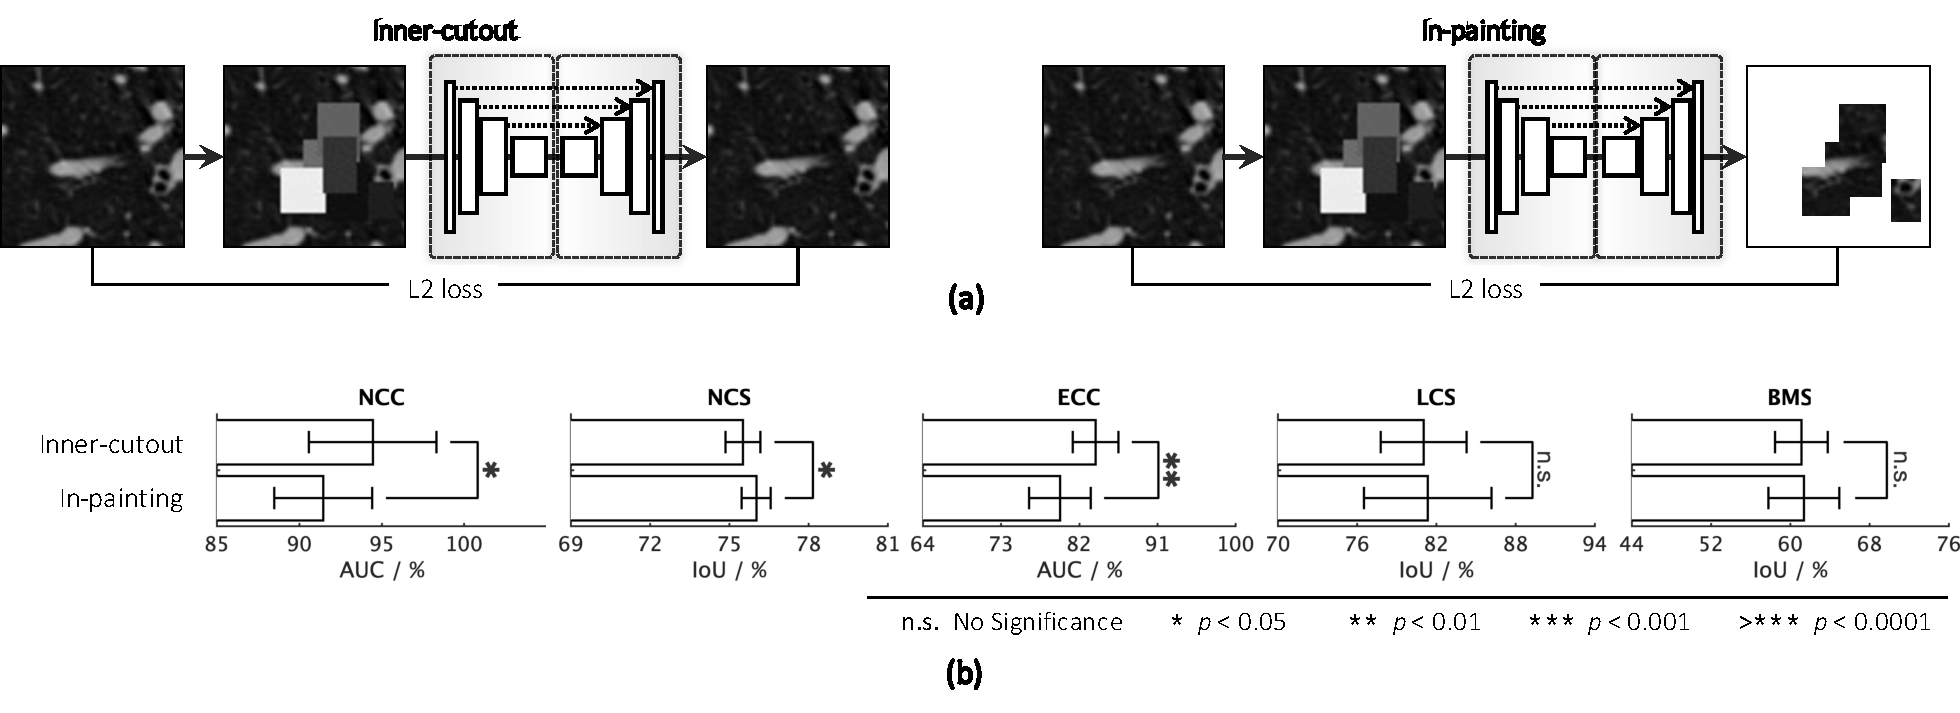
\includegraphics[width=1.0\linewidth]{Figures/AP2/fig_innercutout_inpainting.pdf}
\end{center}
\caption[Comparison Between Image In-painting and Inner-cutout]{
A direct comparison between image in-painting~\citep{pathak2016context} and our inner-cutout. (a) contrasts our inner-cutout with in-painting, wherein the model in the former scheme computes loss on the entire image and the model in the latter scheme computes loss only for the cutout area. (b) presents the performance on five target tasks, showing that inner-cutout is better suited for target classification tasks (\eg \texttt{NCC} and \texttt{ECC}), while in-painting is more helpful for target segmentation tasks (\eg \texttt{NCS}, \texttt{LCS}, and \texttt{BMS}).
}
\label{ap2:fig:innercutout_inpainting}
\end{figure*}

\textit{Extended 3D In-painting:} In our 3D In-painting, which is inspired by its 2D counterpart~\citep{pathak2016context}, the model is trained to in-paint arbitrary cutout regions based on the rest of the sub-volume. A qualitative illustration of the image in-painting task is shown in the right panel of \figurename~\ref{ap2:fig:innercutout_inpainting}(a). To correctly predict missing regions, networks are required to learn local continuities of organs in medical images via interpolation. Unlike the original in-painting, the adversarial loss and discriminator are excluded from our implementation of the 3D version because our primary goal is to empower models with generic representation, rather than generating sharper and realistic sub-volumes. The generator is a 3D U-Net, consisting of an encoder and a decoder. The input of the encoder is a $64\times 64\times 32$ sub-volume that needs to be in-painted. 
Their decoder works differently than our inner-cutout because it predicts the missing region only, and therefore, the loss is just computed on the cutout region---an ablation study on the loss has been further presented in \figurename~\ref{ap2:fig:innercutout_inpainting}.


\textit{Extended 3D Jigsaw:} In our 3D Jigsaw, which is inspired by its 2D counterpart~\citep{noroozi2016unsupervised}, we utilize the implementation by~\citet{taleb20203d}\footnote{\label{foot:3d_self_learning}Self-Supervised 3D Tasks: \href{https://github.com/HealthML/self-supervised-3d-tasks}{github.com/HealthML/self-supervised-3d-tasks}}, wherein the puzzles are created by sampling a $3\times 3\times 3$ grid of 3D patches. Then, these patches are shuffled according to an arbitrary permutation, selected from a set of predefined permutations. This set with size $P=100$ is chosen out of the $(3\times 3\times 3)!$ possible permutations, by following the Hamming distance based algorithm, and each permutation is assigned an index. As a result, the problem is cast as a $P$-way classification task, \ie the model is trained to recognize the applied permutation index, allowing us to solve the 3D puzzles efficiently. We build the classification model by taking the encoder of 3D U-Net and appending a sequence of $fc$ layers. In the implementation, we minimize the cross-entropy loss of the list of extracted puzzles.


\begin{figure}[t]
\begin{center}
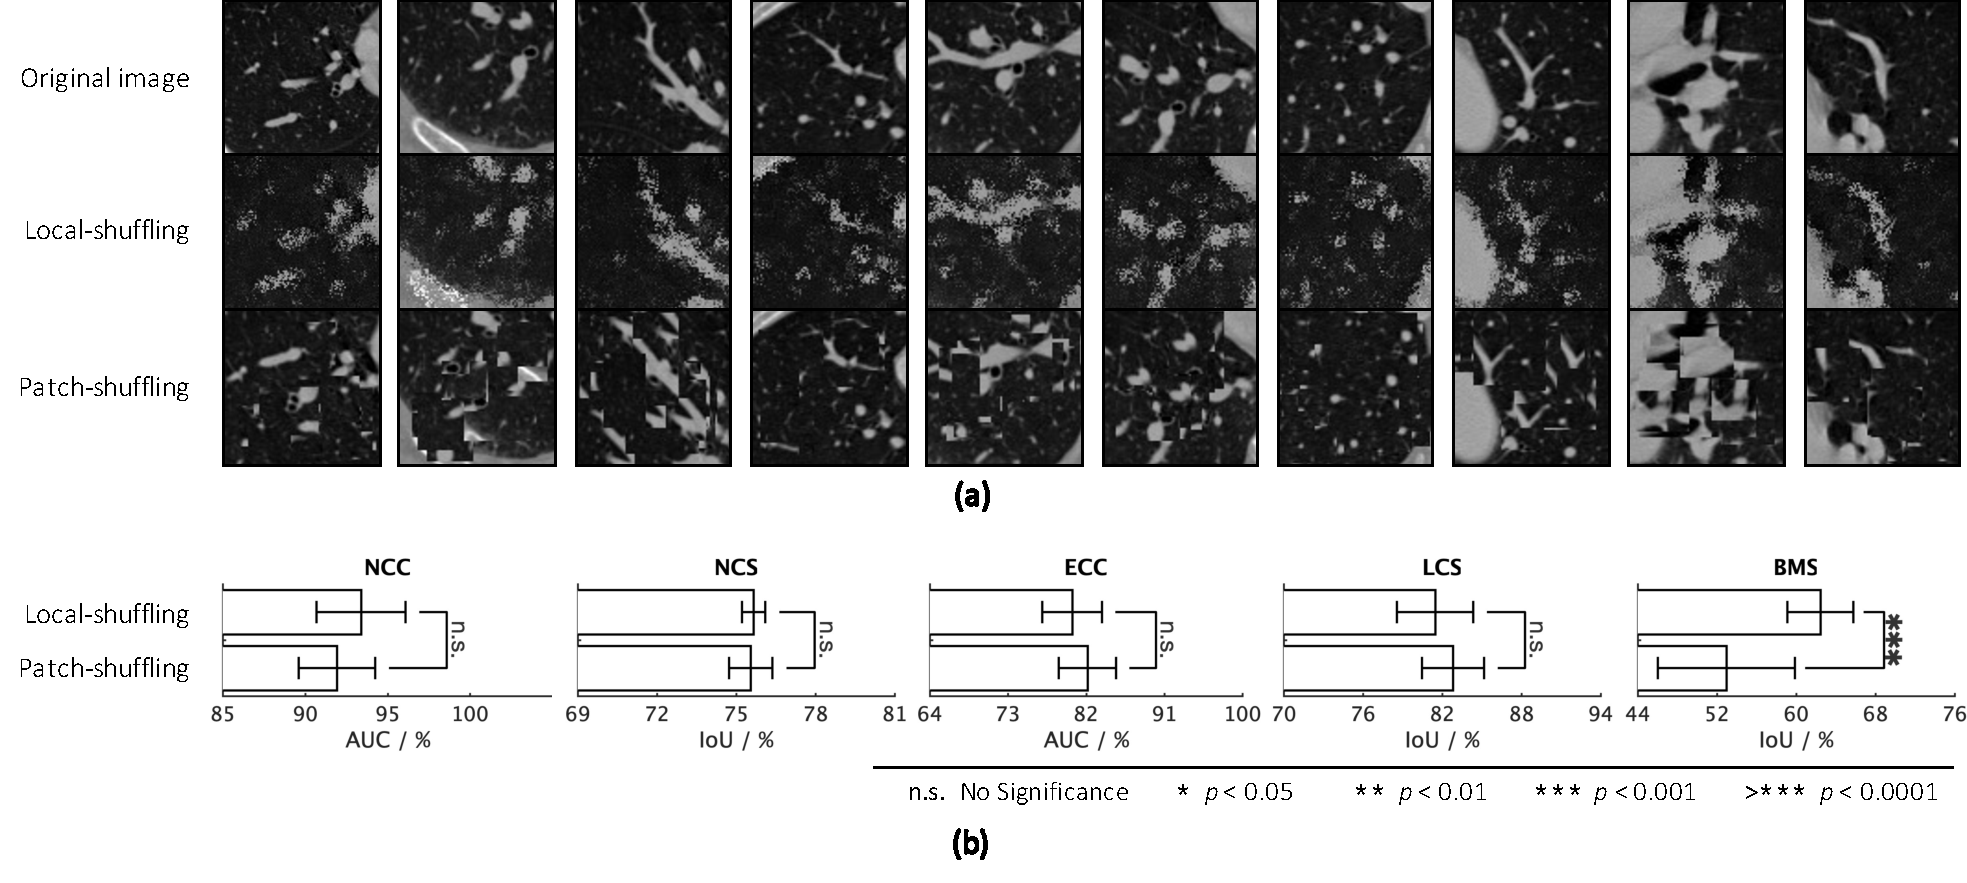
\includegraphics[width=1.0\linewidth]{Figures/AP2/fig_localshuffling_patchshuffling.pdf}
\end{center}
\caption[Comparison Between Global Patch Shuffling and Local Pixel Shuffling]{
A direct comparison between global patch shuffling~\citep{chen2019self} and our local pixel shuffling. (a) illustrates ten example images undergone local-shuffling and patch-shuffling independently. As seen, the overall anatomical structure such as individual organs, blood vessels, lymph nodes, and other soft tissue structures are preserved in the transformed image through local-shuffling.
(b) presents the performance on five target tasks, showing that models pre-trained by our local-shuffling noticeably outperform those pre-trained by patch-shuffling for cross-domain transfer learning (\texttt{BMS}). 
}
\label{ap2:fig:localshuffling_patchshuffling}
\end{figure}

\textit{Extended 3D Patch-shuffling:} In our 3D Patch-shuffling, which is inspired by its 2D counterpart~\citep{chen2019self}, the model learns image representation by restoring the image context. Given a sub-volume, we randomly select two isolated small 3D patches and swap their context. We set the length, width, and height of the 3D patch to be proportional to those in the entire sub-volume by 25\% to 50\%. Repeating this process for $T=10$ times can generate the transformed sub-volume (see examples in \figurename~\ref{ap2:fig:localshuffling_patchshuffling}(a)). The model is trained to restore the original sub-volume, where L2 distance between input and output is used as the loss function. To process volumetric input and ensure a fair comparison with other baselines, we replace their U-Net with 3D U-Net architecture, where the encoder and decoder serve as analysis and restoration parts, respectively.

\textit{Extended 3D DeepCluster:} In our 3D DeepCluster, which is inspired by its 2D counterpart~\citep{caron2018deep}, we iteratively cluster deep features extracted from sub-volumes by $k$-means and use the subsequent assignments as supervision to update the weights of the model. Through clustering, the model can obtain useful general-purpose visual features, requiring little domain knowledge and no specific signal from the inputs. We replaced original AlexNet/VGG architecture with the encoder of 3D U-Net to process 3D input sub-volumes. The number of clusters that works best for 2D tasks may not be a good choice for 3D tasks. To ensure a fair comparison, we extensively tune this hyper-parameter in $\{10,20,40,80,160,320\}$ and finally set to 260 from the narrowed down search space of $\{240,260,280\}$. Unlike ImageNet models for 2D imaging tasks, there is no available pre-trained 3D feature extractor for medical imaging tasks; therefore, we randomly initialize the model weights at the beginning. Our Models Genesis, the first generic 3D pre-trained models, could potentially be used as the 3D feature extractor and co-trained with 3D DeepCluster. 

\textit{Rubik's Cube:} We implement Rubik's Cube with respect to~\citet{zhuang2019self}, which consists of cube rearrangement and cube rotation. Like playing a Rubik's cube, this proxy task enforces models to learn translational and rotational invariant features from raw 3D data. Given a sub-volume, we partition it into a $2\times 2\times 2$ grid of cubes. In addition to predicting orders (3D Jigsaw), this proxy task permutes the cubes with random rotations, forcing models to predict the orientation. Following the original paper, we limit the directions for cube rotation, \ie only allowing 180$^{\circ}$ horizontal and vertical rotations, to reduce the complexity of the task. The eight cubes are then fed into a Siamese network with eight branches sharing the same weight to extract features. The feature maps from the last fully-connected or convolution layer of all branches are concatenated and given as input to the fully-connected layer of separate tasks, \ie cube ordering and orienting, which are supervised by permutation loss and rotation loss, respectively, with equal weights.

\section*{Configurations of Publicly Available Models}
\label{sec:public_3d_model_appendix}

For publicly available models, we do not re-train their proxy tasks and instead simply endeavor to find the best hyper-parameters for each of them in target tasks. We compare them with our Models Genesis in a user perspective, which might seem to be unfair in a research perspective because many variables are asymmetric among the competitors, such as programming platform, model architecture, number of parameters, etc. However, the goal of this section is to experiment with existing ready-to-use pre-trained models under different medical tasks; therefore, we presume that all of the publicly available models and their configurations have been carefully composed to the optimal setting.

\textit{NiftyNet:} We examine the effectiveness of fine-tuning from NiftyNet in five target tasks. We should note that NiftyNet is not initially designed for transfer learning but is one of the few publicly available supervised pre-trained 3D models. The model from~\citet{gibson2018automatic} has been considered as the baseline in our experiments because it has also been pre-trained on the chest region in CT modality and applied an encoder-decoder architecture that is similar to our work. We directly adopt the pre-trained weights of the dense V-Net architecture provided by NiftyNet, so it carries a smaller number of parameters than our 3D U-Net (2.60M vs. 16.32M). For target classification tasks, we use the dense V-Net encoder by appending a sequence of $fc$ layers; for target segmentation tasks, we use the entire dense V-Net. Since NiftyNet is developed in Tensorflow, all five target tasks are re-implemented using their build-in configuration. For each target task, we have tuned hyper-parameters (\eg learning rate and optimizer) and applied extensive data augmentations (\eg rotation and scaling).

\textit{Inflated 3D:} We download the Inflated 3D (I3D) model pre-trained from Flow streams in the Kinetics dataset~\citep{hara2018can} and fine-tune it on our five target tasks. The input sub-volume is copied into two channels to align with the required input shape. For target classification tasks, we take the pre-trained I3D and append a sequence of randomly initialized fully-connected layers. For target segmentation tasks, we take the pre-trained I3D as the encoder and expand a decoder to predict the segmentation map, resulting in a U-Net like architecture. The decoder is the same as that implemented in our 3D U-Net, consisting of up-sampling layers followed by a sequence of convolutional layers, batch normalization, and ReLU activation. Besides, four skip connections are built between the encoder and decoder, wherein feature maps before each pooling layer in the encoder are concatenated with same-scale feature maps in the decoder. All of the layers in the model are trainable during transfer learning. Adam method~\citep{kinga2015method} with a learning rate of $1e-4$ is used for optimization.

\textit{MedicalNet:} We download MedicalNet models~\citep{chen2019med3d} that have been pre-trained on eight publicly available 3D segmentation datasets. ResNet-50 and ResNet-101 backbones are chosen because they are reported by~\citet{chen2019med3d} as the most compelling backbones for target segmentation and classification tasks, respectively. Like I3D, we append a decoder at the end of the pre-trained encoder, randomly initialize its weights, and link the encoder with the decoder using skip connections. Owing to the 3D ResNet backbones, the resultant segmentation network for MedicalNet is much heavier than our 3D U-Net. To be consistent with the original programming platform of MedicalNet, we re-implement all five target tasks in PyTorch, using the same data separation and augmentation. We report the highest results achieved by any of the two backbones in \tablename~\ref{ch5:tab:top_existing_models}.
Zongwei Zhou is currently a Ph.D. candidate in the Department of Biomedical Informatics at Arizona State University (ASU) supervised by Dr. Jianming Liang. Zongwei holds a perfect GPA (4.0/4.0) and has received the University Graduate Fellowship twice from ASU. Drawing upon the realms of biomedical informatics, computer vision, and deep learning, his research focuses on developing novel methodologies to minimize the annotation efforts for computer-aided diagnosis and medical imaging. In addition to 11 U.S. patents pending, Zongwei has published 4 peer-reviewed clinical abstracts and over 10 peer-reviewed journal/conference articles, two of which have received the MICCAI Young Scientist Award and Elsevier-MedIA Best Paper Award. Two of his journal publications have been ranked among the most popular articles in IEEE TMI and the highest-cited article in EJNMMI Research, respectively. Furthermore, Zongwei has been awarded as the co-PI of the Bridges AI program from XSEDE. Zongwei also plays an active role in the leading societies of the computer vision and medical imaging field. He serves as a reviewer of IEEE TPAMI, MedIA, IEEE TMI, etc. and he was on the program committee for MICCAI in 2020, 2021; AAAI in 2020, 2021.
\end{document}
